\documentclass[twoside]{book}

% Packages required by doxygen
\usepackage{calc}
\usepackage{doxygen}
\usepackage{graphicx}
\usepackage[utf8]{inputenc}
\usepackage{makeidx}
\usepackage{multicol}
\usepackage{multirow}
\usepackage{textcomp}
\usepackage[table]{xcolor}

% Font selection
\usepackage[T1]{fontenc}
\usepackage{mathptmx}
\usepackage[scaled=.90]{helvet}
\usepackage{courier}
\usepackage{amssymb}
\usepackage{sectsty}
\renewcommand{\familydefault}{\sfdefault}
\allsectionsfont{%
  \fontseries{bc}\selectfont%
  \color{darkgray}%
}
\renewcommand{\DoxyLabelFont}{%
  \fontseries{bc}\selectfont%
  \color{darkgray}%
}

% Page & text layout
\usepackage{geometry}
\geometry{%
  a4paper,%
  top=2.5cm,%
  bottom=2.5cm,%
  left=2.5cm,%
  right=2.5cm%
}
\tolerance=750
\hfuzz=15pt
\hbadness=750
\setlength{\emergencystretch}{15pt}
\setlength{\parindent}{0cm}
\setlength{\parskip}{0.2cm}
\makeatletter
\renewcommand{\paragraph}{%
  \@startsection{paragraph}{4}{0ex}{-1.0ex}{1.0ex}{%
    \normalfont\normalsize\bfseries\SS@parafont%
  }%
}
\renewcommand{\subparagraph}{%
  \@startsection{subparagraph}{5}{0ex}{-1.0ex}{1.0ex}{%
    \normalfont\normalsize\bfseries\SS@subparafont%
  }%
}
\makeatother

% Headers & footers
\usepackage{fancyhdr}
\pagestyle{fancyplain}
\fancyhead[LE]{\fancyplain{}{\bfseries\thepage}}
\fancyhead[CE]{\fancyplain{}{}}
\fancyhead[RE]{\fancyplain{}{\bfseries\leftmark}}
\fancyhead[LO]{\fancyplain{}{\bfseries\rightmark}}
\fancyhead[CO]{\fancyplain{}{}}
\fancyhead[RO]{\fancyplain{}{\bfseries\thepage}}
\fancyfoot[LE]{\fancyplain{}{}}
\fancyfoot[CE]{\fancyplain{}{}}
\fancyfoot[RE]{\fancyplain{}{\bfseries\scriptsize Generated on Wed Aug 17 2016 11\-:04\-:02 for xtdcpp \mbox{[}common\mbox{]} by Doxygen }}
\fancyfoot[LO]{\fancyplain{}{\bfseries\scriptsize Generated on Wed Aug 17 2016 11\-:04\-:02 for xtdcpp \mbox{[}common\mbox{]} by Doxygen }}
\fancyfoot[CO]{\fancyplain{}{}}
\fancyfoot[RO]{\fancyplain{}{}}
\renewcommand{\footrulewidth}{0.4pt}
\renewcommand{\chaptermark}[1]{%
  \markboth{#1}{}%
}
\renewcommand{\sectionmark}[1]{%
  \markright{\thesection\ #1}%
}

% Indices & bibliography
\usepackage{natbib}
\usepackage[titles]{tocloft}
\setcounter{tocdepth}{3}
\setcounter{secnumdepth}{5}
\makeindex

% Hyperlinks (required, but should be loaded last)
\usepackage{ifpdf}
\ifpdf
  \usepackage[pdftex,pagebackref=true]{hyperref}
\else
  \usepackage[ps2pdf,pagebackref=true]{hyperref}
\fi
\hypersetup{%
  colorlinks=true,%
  linkcolor=blue,%
  citecolor=blue,%
  unicode%
}

% Custom commands
\newcommand{\clearemptydoublepage}{%
  \newpage{\pagestyle{empty}\cleardoublepage}%
}


%===== C O N T E N T S =====

\begin{document}

% Titlepage & ToC
\hypersetup{pageanchor=false}
\pagenumbering{roman}
\begin{titlepage}
\vspace*{7cm}
\begin{center}%
{\Large xtdcpp \mbox{[}common\mbox{]} }\\
\vspace*{1cm}
{\large Generated by Doxygen 1.8.6}\\
\vspace*{0.5cm}
{\small Wed Aug 17 2016 11:04:02}\\
\end{center}
\end{titlepage}
\clearemptydoublepage
\tableofcontents
\clearemptydoublepage
\pagenumbering{arabic}
\hypersetup{pageanchor=true}

%--- Begin generated contents ---
\chapter{Main Page}
\label{index}\hypertarget{index}{}La bibliothèque \hyperlink{namespacextd_1_1network}{xtd\-::network} est la base de toutes les communications réseaux utilisée dans le moteur.

Elle s'appuie sur la bibliothèque boost\-::asio pour fournir des interfaces de haut niveau de client/serveur http et bip (binary-\/protocol).\hypertarget{index_sec_main}{}\section{Sommaire}\label{index_sec_main}


 
\begin{DoxyEnumerate}
\item \hyperlink{index_sec_boost}{Un mot sur boost\-::asio} 
\begin{DoxyEnumerate}
\item \hyperlink{index_ssec_boost_practice}{Les bonnes pratiques}  
\item \hyperlink{index_ssec_boost_bug}{Bug dans la version 1.\-48}  
\end{DoxyEnumerate}


\item \hyperlink{index_sec_design}{Le design} 
\begin{DoxyEnumerate}
\item \hyperlink{index_ssec_design_obj1}{Objectif n°1 \-: mutualiser la gestion des sockets entre client et serveur}  
\item \hyperlink{index_ssec_design_obj2}{Objectif n°2 \-: rester procotole agnostique}  
\end{DoxyEnumerate}


\item \hyperlink{index_sec_bip}{Protocol Bip} 
\begin{DoxyEnumerate}
\item \hyperlink{index_ssec_bip_cnx}{Format et workflow}  
\item \hyperlink{index_ssec_bip_client}{Client bip}  
\item \hyperlink{index_ssec_bip_server}{Serveur bip}  
\end{DoxyEnumerate}


\item \hyperlink{index_sec_http}{Protocol H\-T\-T\-P} 
\begin{DoxyEnumerate}
\item \hyperlink{index_ssec_http_cnx}{Format et workflow}  
\item \hyperlink{index_ssec_http_server}{Serveur http}  
\end{DoxyEnumerate}


\item \hyperlink{index_sec_usages}{Matrice d'utilisation} 


\item \hyperlink{index_sec_tests}{Les tests}  
\end{DoxyEnumerate}\par
\par




 \hypertarget{index_sec_boost}{}\section{Un mot sur boost\-::asio}\label{index_sec_boost}




Boost\-::asio (\href{http://www.boost.org/doc/libs/1_48_0/doc/html/boost_asio.html}{\tt http\-://www.\-boost.\-org/doc/libs/1\-\_\-48\-\_\-0/doc/html/boost\-\_\-asio.\-html}) est une bibliothèque réseau et I/\-O écrite en c++ et utilisée dans de nombreux software.\par
 {\bfseries Son utilisation n'est pas triviale}, aussi la première chose à faire est de bien lire la documentation et se familiariser avec la gestion des événements asynchrones et de l'utilisation du boost\-::asio\-::io\-\_\-service.\par


\par
 \hypertarget{index_ssec_boost_practice}{}\subsection{Les bonnes pratiques}\label{index_ssec_boost_practice}
Pour résumer, on retiendra de la documentation \-:


\begin{DoxyEnumerate}
\item qu'il est fortement {\bfseries déconseillé} de mélanger synchrone et asynchrone
\item qu'il n'est pas possible d'utiliser des timeouts en synchrone. En réalité, on peut fermer la socket pendant l'éxécution d'un événement synchrone mais cette approche n'est pas \char`\"{}naturelle\char`\"{} pour le framework boost\-::asio est cela nous a posé beaucoup de problème en production.
\item qu'il faut, en toutes circonstance, garantir la durée de vie des objets et données utilisée dans les callback des événements asynchrones. L'utilisation des shared\-\_\-ptr sera ici très utile.
\item qu'il est possible de débugguer la gestion des événements à l'aide de la macro {\bfseries -\/\-D\-B\-O\-O\-S\-T\-\_\-\-A\-S\-I\-O\-\_\-\-E\-N\-A\-B\-L\-E\-\_\-\-H\-A\-N\-D\-L\-E\-R\-\_\-\-T\-R\-A\-C\-K\-I\-N\-G} (\href{http://www.boost.org/doc/libs/1_48_0/doc/html/boost_asio/overview/core/handler_tracking.html}{\tt http\-://www.\-boost.\-org/doc/libs/1\-\_\-48\-\_\-0/doc/html/boost\-\_\-asio/overview/core/handler\-\_\-tracking.\-html})
\end{DoxyEnumerate}

\par
 \hypertarget{index_ssec_boost_bug}{}\subsection{Bug dans la version 1.\-48}\label{index_ssec_boost_bug}
Aujourd'hui (18-\/10-\/2013), on utilise boost\-::asio en compilant avec la macro {\bfseries -\/\-D\-B\-O\-O\-S\-T\-\_\-\-A\-S\-I\-O\-\_\-\-D\-I\-S\-A\-B\-L\-E\-\_\-\-E\-P\-O\-L\-L}. Cette macro a pour effet de forcer l'utilisation de l'appel systeme \char`\"{}select\char`\"{} a la place de son jeune remplaçant \char`\"{}epoll\char`\"{}.

Ce point nous a posé énormément de problèmes. Pendant plusieurs semaines, des simples \char`\"{}toy problem\char`\"{} ne marchaient pas dès que le serveur avait plus qu'une thread en écoute sur son boost\-::asio\-::io\-\_\-service. De temps en temps, le client envoyait une requête, les données traversent le réseaux (wireshark) mais le serveur ne déclenche pas son événement de lecture de donnée sur la socket... rien ne se passe et la socket est perdue.

On a jamais trouvé l'explication finale de ce problème, ni de bug précis dans le tracker boost ni d'explication à la lecture du code. Toujours est-\/il qu'un faisceau d'indices nous a fait conclure à une faille de boost\-::asio dans sa gestion du epoll.

Les indices étants \-:
\begin{DoxyItemize}
\item de nombreuse va-\/et-\/vient dans les changelog asio sur le epoll entre la version 1.\-48 (qu'on utilise) et la version 1.\-54 actuelle
\item la disparition de ces problèmes lorsqu'on passe en select
\item la disparition de ces problèmes lorsqu'on passe en boost\-::asio 1.\-52
\end{DoxyItemize}

\par


 \hypertarget{index_sec_design}{}\section{Le design}\label{index_sec_design}




Le design de la bibliothèque \hyperlink{namespacextd_1_1network}{xtd\-::network} est composé de deux couches \-:
\begin{DoxyItemize}
\item la couche haute xtd\-::network\-::protocol qui implémentent les clients serveurs pour les protocoles H\-T\-T\-P et B\-I\-P utilisés dans le moteur
\item la couche basse \hyperlink{namespacextd_1_1network_1_1base}{xtd\-::network\-::base} qui fournie les primitives de bas niveau pour l'implémentation de ces protocoles.
\end{DoxyItemize}\hypertarget{index_ssec_design_obj1}{}\subsection{Objectif n°1 \-: mutualiser la gestion des sockets entre client et serveur}\label{index_ssec_design_obj1}
Pour y parvenir, on crée un objet \char`\"{}\-Connection\char`\"{} qui sera utilisé à la fois dans le client et dans le serveur. Cet objet fera office d'interface avec la socket en proposant des primitives simples d'ouverture, d'envoi et de réception de données.

De plus, cet objet va nous aider dans la gestion du multithreading en garantissant, en travaillant sur son propre boost\-::asio\-::strand, qu'une seule opération soit exécutée à la fois.

On se retrouve donc à définir 3 objets dans cette couche basse \-:
\begin{DoxyItemize}
\item \hyperlink{classxtd_1_1network_1_1base_1_1Connection}{xtd\-::network\-::base\-::\-Connection} \-: un objet s'occupant des interactions avec la socket
\item \hyperlink{classxtd_1_1network_1_1base_1_1Client}{xtd\-::network\-::base\-::\-Client} \-: un client
\item \hyperlink{classxtd_1_1network_1_1base_1_1Server}{xtd\-::network\-::base\-::\-Server} \-: un serveur
\end{DoxyItemize}



On parlera de triplet client/server/connection \-: \hypertarget{index_ssec_design_obj2}{}\subsection{Objectif n°2 \-: rester procotole agnostique}\label{index_ssec_design_obj2}
On définit un protocol comme étant \-:
\begin{DoxyItemize}
\item le format du message échangé \-: quelle langue parlent les deux interlocuteurs et, en particulier, comment font-\/il pour savoir qu'un message est terminé (problème du morcelement des packets par le transport T\-C\-P/\-I\-P).
\item la séquence du dialogue \-: qui commence à parler ? qui commence à écouter ? En tout temps, il faut qu'un interlocuteur écoute lorsque l'autre parle et vis/versa.
\end{DoxyItemize}

Pour rester agnostique du protocol, notre triplet (client, server, connexion) ne doit pas faire de supposition ni le format du message ni sur l'enchaînement des envois et des réceptions. En ce qui concerne le format, cela implique que la \hyperlink{classxtd_1_1network_1_1base_1_1Connection}{xtd\-::network\-::base\-::\-Connection} ne peut pas directement écrire et lire sur la socket. Dans certains cas, on voudra lire une donnée de taille fixe, dans d'autres cas, un header puis une data, bref, on il faut déléguer ces opérations à la couche xtd\-::network\-::protocol. En ce qui concerne l'enchainement des envois/receptions, cela implique que ces objets ne peuvent pas lancer une réception ou un envoi, ils ne peuvent que définir ces primitives mais sans jamais les appeler.

Au final, on se retrouve avec \-:


\begin{DoxyItemize}
\item \hyperlink{classxtd_1_1network_1_1base_1_1Connection}{xtd\-::network\-::base\-::\-Connection} \-:
\begin{DoxyItemize}
\item ownership de la socket
\item gestion des envois de message avec timeout (partie abstraite de création et mise sur le socket du message)
\item gestion des réceptions de message avec timeout (partie abstraite de décodage et lecture sur le socket du message)
\item gestion ouverture et fermeture de la socket
\end{DoxyItemize}
\item \hyperlink{classxtd_1_1network_1_1base_1_1Client}{xtd\-::network\-::base\-::\-Client} \-:
\begin{DoxyItemize}
\item gère l'instanciation d'un connexion
\item la connexion vers un serveur (utilise \hyperlink{classxtd_1_1network_1_1base_1_1Connection_a408b83f0e43d18e32f31d6c13d6dcdf3}{xtd\-::network\-::base\-::\-Connection\-::connect})
\item l'envoie d'un message (utilise \hyperlink{classxtd_1_1network_1_1base_1_1Connection_a8ebc5958cf7d27a902bd75a55c4648bf}{xtd\-::network\-::base\-::\-Connection\-::send})
\item la réception d'un message (utilise \hyperlink{classxtd_1_1network_1_1base_1_1Connection_a09146c9c2dbf1ad85867fd0afab15c0c}{xtd\-::network\-::base\-::\-Connection\-::receive})
\item la fermeture de la connexion (utilise \hyperlink{classxtd_1_1network_1_1base_1_1Connection_a73097d339a3716c05fee7ee19753ee4a}{xtd\-::network\-::base\-::\-Connection\-::close})
\item les compteurs d'exploitation
\end{DoxyItemize}
\item \hyperlink{classxtd_1_1network_1_1base_1_1Server}{xtd\-::network\-::base\-::\-Server} \-:
\begin{DoxyItemize}
\item l'initialisation des threads de traitement et de connexion
\item l'ouverture d'une connexion entrante (utilise \hyperlink{classxtd_1_1network_1_1base_1_1Connection_af8da803db4caa1f125548508cf3db134}{xtd\-::network\-::base\-::\-Connection\-::accept})
\item réception d'un message (utilise \hyperlink{classxtd_1_1network_1_1base_1_1Connection_a09146c9c2dbf1ad85867fd0afab15c0c}{xtd\-::network\-::base\-::\-Connection\-::receive})
\item envoie d'un message (utilise \hyperlink{classxtd_1_1network_1_1base_1_1Connection_a8ebc5958cf7d27a902bd75a55c4648bf}{xtd\-::network\-::base\-::\-Connection\-::send})
\item fermeture des connexion (utilise \hyperlink{classxtd_1_1network_1_1base_1_1Connection_a73097d339a3716c05fee7ee19753ee4a}{xtd\-::network\-::base\-::\-Connection\-::close})
\item les compteurs d'exploitation
\end{DoxyItemize}
\end{DoxyItemize}

Ensuite, chaque protocole n'a plus qu'a définir ses spécificités en créant son propre son triplet de client/server/connexion qui dérive du triplet de base.\par
 Au final ou abouti au modèle suivant \-:



\par


 \hypertarget{index_sec_bip}{}\section{Protocol Bip}\label{index_sec_bip}




\par
 \hypertarget{index_ssec_bip_cnx}{}\subsection{Format et workflow}\label{index_ssec_bip_cnx}
\subsection*{Format }

Un message bip est composé de deux parties \-:
\begin{DoxyItemize}
\item un header \-: une suite de Connection\-::mcs\-\_\-header\-Size uint32\-\_\-t (donc taille fixe)
\item une data \-: une suite de taille variable de uint8
\item un crc de data \-: un crc en uint8 calculé sur les Connection\-::mcs\-\_\-max\-Data\-Crc\-Size derniers octects de la partie donnée.
\end{DoxyItemize}

Le header embarque 3 informations \-:
\begin{DoxyItemize}
\item la taille de la partie donnée (comptabilise le crc finale) en nombre d'octect
\item un identifiant de requête croissant (s'incrémente à chaque requete)
\item un crc de header calculé sur les (Connection\-::mcs\-\_\-header\-Size -\/ 1) unit32 du header
\end{DoxyItemize}

A la réception \-:
\begin{DoxyItemize}
\item on commence par lire le header
\item on vérifie l'integrité du header en comparant le crc de header reçu et le crc du header re-\/calculé
\item on extrait la taille du message N attendu a partir du header, on on va lire sur la socket ces N octects.
\end{DoxyItemize}

A la réception de la partie donnée \-:
\begin{DoxyItemize}
\item on vérifie l'intégrité du message en comparant le crc de donnée contenu dans dernier octet du message au crc recalculé.
\end{DoxyItemize}

\subsection*{Séquence de dialogue }



\par
 \hypertarget{index_ssec_bip_client}{}\subsection{Client bip}\label{index_ssec_bip_client}

\begin{DoxyParams}{Parameters}
{\em T\-Domain} & \-: mode de connexion, utils\-::af\-\_\-inet ou utils\-::af\-\_\-unix \\
\hline
{\em T\-Request} & Structure requète serialisable avec boost\-::serialization \\
\hline
{\em T\-Response} & Structure réponse serialisable avec boost\-::serialization\\
\hline
\end{DoxyParams}
Client générique bip \-: gère l'envoi de structure T\-Request et la réception de structure T\-Response vers un serveur bip de même type.

Selon la configuration transmise au constructeur, les données pourront etre compressées avant l'envoi et décompressée à la réception.

La méthode send de cet objet est non bloquante et déclenche, en interne, la réception de la réponse du serveur. La méthode receive, elle, est bloquante jusqu'à la réception effective de la réponse. Cette approche permet à un utilisateur, qui aurait plusieurs client connectés vers plusieurs serveurs, d'envoyer ses requètes et de réceptionner en parallèle ses réponses pour au final aller au rythme du serveur le plus lent et pas subir la somme de tous les temps de réponse.

Thread safety \-:
\begin{DoxyItemize}
\item même instance \-: non
\item instances différentes \-: oui
\end{DoxyItemize}

\par
 \hypertarget{index_ssec_bip_server}{}\subsection{Serveur bip}\label{index_ssec_bip_server}

\begin{DoxyParams}{Parameters}
{\em Domain} & \-: mode de connexion, utils\-::af\-\_\-inet ou utils\-::af\-\_\-unix \\
\hline
{\em T\-Req} & \-: Structure requête serialisable avec boost\-::serialization \\
\hline
{\em T\-Res} & \-: Structure réponse serialisable avec boost\-::serialization\\
\hline
\end{DoxyParams}
Serveur générique bip \-: gère la réception de structure T\-Request et l'envoi de structure T\-Response vers un client bip de même type.

Cet objet est destiné à être hérité des différents serveurs qui souhaitent communiquer en bip, ces derniers n'ont qu'a implémenter la méthode virtuelle pure Server\-::process\-Object\-Request pour calculer la réponse à envoyer à partir de la requête reçue

\par


 \hypertarget{index_sec_http}{}\section{Protocol H\-T\-T\-P}\label{index_sec_http}




\par
 \hypertarget{index_ssec_http_cnx}{}\subsection{Format et workflow}\label{index_ssec_http_cnx}
Le protocol http implémenté ici gère les version 1.\-0 et une sous-\/partie de la version 1.\-1 des spécifications données par le W3\-C. \subsection*{Format}

Un message H\-T\-T\-P est composé de deux parties \-:
\begin{DoxyItemize}
\item un header \-: une suite de caractère ascii de taille variable terminant par une ligne vide (donc identifiable par la séquence d'octets \char`\"{}\-C\-R-\/\-L\-F-\/\-C\-R-\/\-L\-R\char`\"{})
\item une data \-: une suite de caractère ascii de taille variable, optionnelle et potentiellement encodée dans différents formats
\end{DoxyItemize}

Sans rentrer dans le détail du format du header, ce qui nous intéresse ici c'est que, lorsqu'une data est envoyée, il contient une directive {\bfseries Content-\/\-Length} qui renseigne sur la taille en octet de la data.

A la réception, on lit des données par petits bouts jusqu'à trouver la fin du header (ligne vide), on extrait ensuite la taille de la donnée et, si elle présente et est non-\/nulle, on se met à lire jusqu'à avoir suffisamment d'octets.

Pour des raisons pratique, le parsing du header et la récupération de la taille de la data est déléguée à l'objet \hyperlink{classxtd_1_1network_1_1http_1_1Request}{xtd\-::network\-::http\-::\-Request}

\subsection*{Séquence de dialogue }



\par
 \hypertarget{index_ssec_http_server}{}\subsection{Serveur http}\label{index_ssec_http_server}
\par
\par
 
\begin{DoxyParams}{Parameters}
{\em Domain} & mode de connexion, utils\-::af\-\_\-inet ou utils\-::af\-\_\-unix\\
\hline
\end{DoxyParams}
Serveur générique http. Gère la réception de requête H\-T\-T\-P, les transforme en objet Request, et envoie des réponses H\-T\-T\-P à partir d'objet Response.

En interne, cet objet gère une liste de \char`\"{}handlers\char`\"{}, capables de transformer un objet Request en un objet Response. Il gère également un mécanisme d'enregistrement et de routage des requête ces différents handlers.

\par
 \subsection*{Le routage }

Le routage est extrêmement simple. On pacourt la liste des handlers enregistrés, et on exécute le premier vérifiant toutes les conditions. Si aucun handler est trouvé, on exécute le handler par défaut.

Pour être exécuté, un handler doit remplir deux critère \-:
\begin{DoxyItemize}
\item l'url sur laquelle il à été enregistré correspond a la ressource demandée dans la requête (ce qui suit le G\-E\-T ou le P\-O\-S\-T de la première ligne du header). On note le cas spécial où un handler peut être enregistré sur toutes les urls en même temps.
\item si le handler a été enregistré avec un filtre, on vérifie la condition posée le filtre est vrai pour la requête.
\end{DoxyItemize}

\par
 \subsection*{Les handlers }

Un handler doit être vu comme un pointeur sur fonction dont le prototype serait \-: 
\begin{DoxyCode}
status myhandler(uint32\_t p\_requestID, \textcolor{keyword}{const} Request& p\_req, Response& p\_res);
\end{DoxyCode}


En réalité, cet objet demande à ce que les handlers soient construit à partir de ses classes internes, dont le raccourcis est \char`\"{}h\char`\"{}. Exemple \-: 
\begin{DoxyCode}
\textcolor{comment}{// une fonction à moi que j'aime}
status MyServer::myhandler(uint32\_t p\_requestID, \textcolor{keyword}{const} Request& p\_req, Response& p\_res);

\textcolor{comment}{// enregistrement de ma fonction comme handler de la ressources /index}
bind(\textcolor{stringliteral}{"/index"}, h(&MyServer::myhandler, \textcolor{keyword}{this}));
\end{DoxyCode}


La raison pour laquelle ces handlers ont été wrappé dans un objet interne est d'une part de ne pas demander à l'utilisateur de systématiquement binder 3 placeholders \-\_\-1, \-\_\-2, \-\_\-3.

\par
 \subsection*{Les filtres }

De la même façon, les filtres doivent être vus comme un pointeur sur fonction dont le prototype serait \-: 
\begin{DoxyCode}
\textcolor{keywordtype}{bool} filter(\textcolor{keyword}{const} Request&);
\end{DoxyCode}


Ils se contruisent à partir de l'objet interne du server dont le raccourcis est \char`\"{}f\char`\"{}. Exemple \-: 
\begin{DoxyCode}
\textcolor{comment}{// une fonction à moi que j'aime}
status MyServer::myhandler(uint32\_t p\_requestID, \textcolor{keyword}{const} Request& p\_req, Response& p\_res);
\textcolor{keywordtype}{bool}  MyServer::myfilter(\textcolor{keyword}{const} Request& p\_req);

\textcolor{comment}{// enregistrement de ma fonction comme handler de la ressources /index}
bind(\textcolor{stringliteral}{"/index"}, h(&MyServer::myhandler, \textcolor{keyword}{this}), f(&MyServer::myfilter, \textcolor{keyword}{this}));
\end{DoxyCode}


Ils ont également une autre fonctionnalité, il peuvent se composer avec les opérateurs standards booléens $\vert$$\vert$, \&\& et !. Exemple \-:


\begin{DoxyCode}
\textcolor{comment}{// une fonction à moi que j'aime}
status MyServer::myhandler(uint32\_t p\_requestID, \textcolor{keyword}{const} Request& p\_req, Response& p\_res);
\textcolor{keywordtype}{bool}  MyServer::hasHeader(\textcolor{keyword}{const} \textcolor{keywordtype}{string}& p\_headerName, \textcolor{keyword}{const} Request& p\_req)
\{
  \textcolor{keywordflow}{return} p\_req.existsHeader(p\_headerName);
\}

\textcolor{comment}{// enregistrement de ma fonction comme handler de la ressources /index}
bind(\textcolor{stringliteral}{"/index"},
     h(&MyServer::myhandler, \textcolor{keyword}{this}),
     f(&MyServer::hasHeader, \textcolor{keyword}{this}, \textcolor{stringliteral}{"Content-type"}) &&
     f(&MyServer::hasHeader, \textcolor{keyword}{this}, \textcolor{stringliteral}{"Content-Length"}));
\end{DoxyCode}


\par
 \subsection*{L'enregistrement }

Cet objet founi de nombreuses méthodes utilitaires pour faciliter l'enregistrement des handlers. Elles sont toutes préfixées par \char`\"{}bind\char`\"{}.


\begin{DoxyItemize}
\item 
\begin{DoxyCode}
\textcolor{keywordtype}{void} bind(\textcolor{keyword}{const} \textcolor{keywordtype}{string}& p\_url, handler p\_handler, [filter p\_filter]); 
\end{DoxyCode}
 
\begin{DoxyParams}{Parameters}
{\em p\-\_\-url} & ressource à enregistrer \\
\hline
{\em p\-\_\-handler} & handler à enregistrer \\
\hline
{\em p\-\_\-filter} & filter \char`\"{}filtre\char`\"{} optionnel \\
\hline
{\em p\-\_\-descr} & description du handler (optionnel)\\
\hline
\end{DoxyParams}
Enregistrement générique de la ressource p\-\_\-url sous condition optionnelle p\-\_\-filter sur le handler p\-\_\-handler. \par
\par

\item 
\begin{DoxyCode}
\textcolor{keywordtype}{void} bind\_any(handler p\_handler, [filter p\_filter]); 
\end{DoxyCode}
 \par
\par
 
\begin{DoxyParams}{Parameters}
{\em p\-\_\-handler} & handler à enregistrer \\
\hline
{\em p\-\_\-filter} & filter \char`\"{}filtre\char`\"{} optionnel\\
\hline
\end{DoxyParams}
Comme \hyperlink{classxtd_1_1network_1_1http_1_1Server_a7281ae7cdda6d7b2334b27e530ce000f}{xtd\-::network\-::http\-::\-Server\-::bind} mais se déclenche quelque soit la ressource demandée. \par
\par

\item 
\begin{DoxyCode}
\textcolor{keywordtype}{void} bind\_default(handler p\_handler); 
\end{DoxyCode}
 \par
\par
 
\begin{DoxyParams}{Parameters}
{\em p\-\_\-handler} & handler à enregistrer\\
\hline
\end{DoxyParams}
Enregistrement du handler à exécuter lorsqu'aucun handler valide n'a été trouvé. A la construction, le handler par défaut est Server\-::h\-\_\-error\-\_\-template. \par
\par

\item 
\begin{DoxyCode}
\textcolor{keywordtype}{void} bind\_redirect(\textcolor{keyword}{const} \textcolor{keywordtype}{string}& p\_src, \textcolor{keyword}{const} \textcolor{keywordtype}{string}& p\_dst, [filter p\_filter]); 
\end{DoxyCode}
 \par
\par
 
\begin{DoxyParams}{Parameters}
{\em p\-\_\-src} & ressource sur laquelle déclencher la redirection \\
\hline
{\em p\-\_\-dst} & destination de la redirection \\
\hline
{\em p\-\_\-filter} & filter \char`\"{}filtre\char`\"{} optionnel\\
\hline
\end{DoxyParams}
Enregistrement d'un handler de redirection. Créer une réponse http qui contient le header \char`\"{}\-Location \-: p\-\_\-dst\char`\"{} et le code H\-T\-T\-P Response\-::\-S\-T\-A\-T\-U\-S\-\_\-302. \par
\par

\item 
\begin{DoxyCode}
\textcolor{keywordtype}{void} bind\_file(\textcolor{keyword}{const} \textcolor{keywordtype}{string}& p\_path,
               \textcolor{keyword}{const} \textcolor{keywordtype}{string}& p\_filePath,
               \textcolor{keyword}{const} \textcolor{keywordtype}{string}& p\_contentType = \textcolor{stringliteral}{"text/plain"},
               [filter            p\_filter]);
\end{DoxyCode}
 \par
\par
 Voir \hyperlink{classxtd_1_1network_1_1http_1_1Server_a4358a20d2246a84f67d299f385c5bce8}{xtd\-::network\-::http\-::\-Server\-::h\-\_\-file} \par
\par

\item 
\begin{DoxyCode}
\textcolor{keywordtype}{void} bind\_dir(\textcolor{keyword}{const} \textcolor{keywordtype}{string}& p\_path,
              \textcolor{keyword}{const} \textcolor{keywordtype}{string}& p\_filePath,
              \textcolor{keyword}{const} \textcolor{keywordtype}{string}& p\_contentType = \textcolor{stringliteral}{"text/plain"},
              [filter            p\_filter]);
\end{DoxyCode}
 \par
\par
 Voir \hyperlink{classxtd_1_1network_1_1http_1_1Server_a71d7415223786f5451ef36f62c91782e}{xtd\-::network\-::http\-::\-Server\-::h\-\_\-dir} \par
\par

\end{DoxyItemize}

\subsection*{Les handlers prédéfinis }


\begin{DoxyItemize}
\item 
\begin{DoxyCode}
h\_redirect(\textcolor{keyword}{const} \textcolor{keywordtype}{string}& p\_dst, \textcolor{keyword}{const} uint32\_t p\_requestId, \textcolor{keyword}{const} Request& p\_request, Response& p\_response)
      ; 
\end{DoxyCode}
 Handler de redirection. 
\begin{DoxyParams}{Parameters}
{\em p\-\_\-dst} & destination de la redirection H\-T\-T\-P \\
\hline
{\em p\-\_\-request\-Id} & identifiant de requête \\
\hline
{\em p\-\_\-request} & \hyperlink{classxtd_1_1network_1_1http_1_1Request}{requête} \\
\hline
{\em p\-\_\-response} & \hyperlink{classxtd_1_1network_1_1http_1_1Response}{réponse}\\
\hline
\end{DoxyParams}
Créer une redirection H\-T\-T\-P Response\-::\-S\-T\-A\-T\-U\-S\-\_\-302 \char`\"{}code 302\char`\"{} redirigeant sur p\-\_\-dst
\item 
\begin{DoxyCode}
h\_raw(\textcolor{keyword}{const} \textcolor{keywordtype}{string}& p\_data, \textcolor{keyword}{const} \textcolor{keywordtype}{string}& p\_contentType, \textcolor{keyword}{const} uint32\_t p\_requestId, \textcolor{keyword}{const} Request& 
      p\_request, Response& p\_response); 
\end{DoxyCode}
 Handler de contenu. 
\begin{DoxyParams}{Parameters}
{\em p\-\_\-data} & donnée à insérer dans la réponse \\
\hline
{\em p\-\_\-content\-Type} & type M\-I\-M\-E de la donnée \\
\hline
{\em p\-\_\-response} & \hyperlink{classxtd_1_1network_1_1http_1_1Response}{réponse}\\
\hline
\end{DoxyParams}
Créer une réponse H\-T\-T\-P (Response\-::\-S\-T\-A\-T\-U\-S\-\_\-200 contenant la donnée p\-\_\-data et le header {\bfseries Content-\/\-Type} p\-\_\-content\-Type
\item 
\begin{DoxyCode}
h\_file(\textcolor{keyword}{const} \textcolor{keywordtype}{string}& p\_filePath, \textcolor{keyword}{const} \textcolor{keywordtype}{string}& p\_contentType, \textcolor{keyword}{const} uint32\_t p\_requestId, \textcolor{keyword}{const} Request& 
      p\_request, Response& p\_response); 
\end{DoxyCode}
 Handler de fichier. 
\begin{DoxyParams}{Parameters}
{\em p\-\_\-file\-Path} & chemin vers le fichier à insérer dans la réponse \\
\hline
{\em p\-\_\-content\-Type} & type M\-I\-M\-E du fichier \\
\hline
{\em p\-\_\-cachable} & La reponse peut elle mettre en mis en cache par le navigateur ? \\
\hline
{\em p\-\_\-request\-Id} & identifiant de requête \\
\hline
{\em p\-\_\-request} & \hyperlink{classxtd_1_1network_1_1http_1_1Request}{requête} \\
\hline
{\em p\-\_\-response} & \hyperlink{classxtd_1_1network_1_1http_1_1Response}{réponse}\\
\hline
\end{DoxyParams}
Créer une réponse H\-T\-T\-P Response\-::\-S\-T\-A\-T\-U\-S\-\_\-200 embarquant le contenu du fichier pointé par p\-\_\-file\-Path et le header {\bfseries Content-\/\-Type} p\-\_\-content\-Type. Si p\-\_\-file\-Path n'éxiste pas, la réponse sera générée par \hyperlink{classxtd_1_1network_1_1http_1_1Server_a39656db929894be1af465c0409c22f35}{xtd\-::network\-::http\-::\-Server\-::h\-\_\-error\-\_\-text}.
\item 
\begin{DoxyCode}
h\_dir(\textcolor{keyword}{const} \textcolor{keywordtype}{string}& p\_dirPath, \textcolor{keyword}{const} \textcolor{keywordtype}{string}& p\_contentType, \textcolor{keyword}{const} uint32\_t p\_requestId, \textcolor{keyword}{const} Request& 
      p\_request, Response& p\_response); 
\end{DoxyCode}
 Handler de répertoire. 
\begin{DoxyParams}{Parameters}
{\em p\-\_\-dir\-Path} & chemin vers le répertoire à servir \\
\hline
{\em p\-\_\-content\-Type} & type M\-I\-M\-E des fichiers du répertoire \\
\hline
{\em p\-\_\-cachable} & La reponse peut elle mettre en mis en cache par le navigateur ? \\
\hline
{\em p\-\_\-request\-Id} & identifiant de requête \\
\hline
{\em p\-\_\-request} & \hyperlink{classxtd_1_1network_1_1http_1_1Request}{requête} \\
\hline
{\em p\-\_\-response} & \hyperlink{classxtd_1_1network_1_1http_1_1Response}{réponse}\\
\hline
\end{DoxyParams}
Comme \hyperlink{classxtd_1_1network_1_1http_1_1Server_a4358a20d2246a84f67d299f385c5bce8}{xtd\-::network\-::http\-::\-Server\-::h\-\_\-file} mais trouve automatiquement quel fichier de p\-\_\-dir\-Path à servir en fonction de la ressource demandé dans p\-\_\-request.
\item 
\begin{DoxyCode}
h\_template\_file(\textcolor{keyword}{const} Template& p\_tmpl, \textcolor{keyword}{const} \textcolor{keywordtype}{string}& \textcolor{keyword}{const} uint32\_t p\_requestID, \textcolor{keyword}{const} Request& p\_request,
       Response& p\_response); 
\end{DoxyCode}
 Handler de texte templaté a partir d'un fichier. 
\begin{DoxyParams}{Parameters}
{\em p\-\_\-tmpl} & objet \hyperlink{classxtd_1_1network_1_1http_1_1Template}{template} \\
\hline
{\em p\-\_\-file\-Path} & fichier a partir duquel initialiser le template \\
\hline
{\em p\-\_\-request\-I\-D} & identifiant de requête \\
\hline
{\em p\-\_\-req} & \hyperlink{classxtd_1_1network_1_1http_1_1Request}{requête} \\
\hline
{\em p\-\_\-res} & \hyperlink{classxtd_1_1network_1_1http_1_1Response}{réponse}\\
\hline
\end{DoxyParams}
Génère une réponse H\-T\-T\-P pré-\/formatée par l'objet Template p\-\_\-tmpl Response\-::\-S\-T\-A\-T\-U\-S\-\_\-200. Le header {\bfseries Content-\/\-Type} est également donné par p\-\_\-tmpl. Si la lecture du fichier p\-\_\-file\-Path ou si la résolution des variable du template échouent, alors la réponse sera générée par \hyperlink{classxtd_1_1network_1_1http_1_1Server_a39656db929894be1af465c0409c22f35}{xtd\-::network\-::http\-::\-Server\-::h\-\_\-error\-\_\-text}.
\item 
\begin{DoxyCode}
h\_error\_text(\textcolor{keyword}{const} \textcolor{keywordtype}{string}& p\_message, \textcolor{keyword}{const} uint32\_t p\_requestId, \textcolor{keyword}{const} Request& p\_request, Response& 
      p\_response); 
\end{DoxyCode}
 Handler de génération de message d'erreur en texte. 
\begin{DoxyParams}{Parameters}
{\em p\-\_\-message} & contenu du message d'erreur \\
\hline
{\em p\-\_\-request\-Id} & identifiant de requête \\
\hline
{\em p\-\_\-request} & \hyperlink{classxtd_1_1network_1_1http_1_1Request}{requête} \\
\hline
{\em p\-\_\-response} & \hyperlink{classxtd_1_1network_1_1http_1_1Response}{réponse}\\
\hline
\end{DoxyParams}
Génère une réponse H\-T\-T\-P d'erreur Response\-::\-S\-T\-A\-T\-U\-S\-\_\-500 de type {\bfseries Content-\/\-Type} \char`\"{}text/plain\char`\"{} contenant le message p\-\_\-message.
\item 
\begin{DoxyCode}
h\_error\_html(\textcolor{keyword}{const} \textcolor{keywordtype}{string}& p\_message, \textcolor{keyword}{const} uint32\_t p\_requestId, \textcolor{keyword}{const} Request& p\_request, Response& 
      p\_response); 
\end{DoxyCode}
 Handler de génération de message d'erreur en html. 
\begin{DoxyParams}{Parameters}
{\em p\-\_\-message} & contenu du message d'erreur \\
\hline
{\em p\-\_\-request\-Id} & identifiant de requête \\
\hline
{\em p\-\_\-request} & \hyperlink{classxtd_1_1network_1_1http_1_1Request}{requête} \\
\hline
{\em p\-\_\-response} & \hyperlink{classxtd_1_1network_1_1http_1_1Response}{réponse}\\
\hline
\end{DoxyParams}
Même chose que \hyperlink{classxtd_1_1network_1_1http_1_1Server_a39656db929894be1af465c0409c22f35}{xtd\-::network\-::http\-::\-Server\-::h\-\_\-error\-\_\-text} mais le méssage généré est de type \char`\"{}text/html\char`\"{}.
\end{DoxyItemize}

\subsection*{Les filtres prédéfinis }


\begin{DoxyItemize}
\item 
\begin{DoxyCode}
\textcolor{keyword}{static} \textcolor{keywordtype}{bool} f\_none(\textcolor{keyword}{const} Request& p\_request); 
\end{DoxyCode}
 Toujours vrai. \par
\par
 \par
\par

\item 
\begin{DoxyCode}
\textcolor{keywordtype}{bool} f\_cgi\_exist(\textcolor{keyword}{const} \textcolor{keywordtype}{string}& p\_cgiName, \textcolor{keyword}{const} Request& p\_request); 
\end{DoxyCode}
 Vrai si la requête contient un paramètre G\-E\-T nommé p\-\_\-cgi\-Name. \par
\par
 \par
\par

\item 
\begin{DoxyCode}
\textcolor{keywordtype}{bool} f\_one\_cgi\_exist(\textcolor{keyword}{const} vector <string > & p\_cgiName, \textcolor{keyword}{const} Request& p\_req); 
\end{DoxyCode}
 \par
\par
 Vrai si la requête contient un paramètre G\-E\-T dont le nom correspond à l'un des éléments du tableau p\-\_\-cgi\-Name \par
\par

\item 
\begin{DoxyCode}
\textcolor{keywordtype}{bool} f\_cgi\_equal(\textcolor{keyword}{const} \textcolor{keywordtype}{string}& p\_cgiName, \textcolor{keyword}{const} \textcolor{keywordtype}{string}& p\_value, \textcolor{keyword}{const} Request& p\_request); 
\end{DoxyCode}
 \par
\par
 Vrai si la requête contient un paramètre G\-E\-T nommé p\-\_\-cgi\-Name et dont la valeur est égale à p\-\_\-value \par
\par

\item 
\begin{DoxyCode}
\textcolor{keywordtype}{bool} f\_cgi\_match(\textcolor{keyword}{const} \textcolor{keywordtype}{string}& p\_cgiName, \textcolor{keyword}{const} \textcolor{keywordtype}{string}& p\_regex, \textcolor{keyword}{const} Request& p\_request); 
\end{DoxyCode}
 \par
\par
 Vrai si la requête contient un paramètre G\-E\-T nommé p\-\_\-cgi\-Name et dont la valeur match la regexp p\-\_\-regex \par
\par

\item 
\begin{DoxyCode}
\textcolor{keywordtype}{bool} f\_post\_exist(\textcolor{keyword}{const} \textcolor{keywordtype}{string}& p\_cgiName, \textcolor{keyword}{const} Request& p\_request); 
\end{DoxyCode}
 Vrai si la requête contient un paramètre P\-O\-S\-T nommé p\-\_\-cgi\-Name. \par
\par
 \par
\par

\item 
\begin{DoxyCode}
\textcolor{keywordtype}{bool} f\_post\_equal(\textcolor{keyword}{const} \textcolor{keywordtype}{string}& p\_cgiName, \textcolor{keyword}{const} \textcolor{keywordtype}{string}& p\_value, \textcolor{keyword}{const} Request& p\_request); 
\end{DoxyCode}
 \par
\par
 Vrai si la requête contient un paramètre P\-O\-S\-T nommé p\-\_\-cgi\-Name et dont la valeur est égale à p\-\_\-value \par
\par

\item 
\begin{DoxyCode}
\textcolor{keywordtype}{bool} f\_post\_match(\textcolor{keyword}{const} \textcolor{keywordtype}{string}& p\_cgiName, \textcolor{keyword}{const} \textcolor{keywordtype}{string}& p\_regex, \textcolor{keyword}{const} Request& p\_request); 
\end{DoxyCode}
 \par
\par
 Vrai si la requête contient un paramètre P\-O\-S\-T nommé p\-\_\-cgi\-Name et dont la valeur match la regexp p\-\_\-regex \par
\par

\item 
\begin{DoxyCode}
\textcolor{keywordtype}{bool} f\_header\_exist(\textcolor{keyword}{const} \textcolor{keywordtype}{string}& p\_headerName, \textcolor{keyword}{const} Request& p\_request); 
\end{DoxyCode}
 Vrai si p\-\_\-request contient le header p\-\_\-header\-Name. \par
\par
 \par
\par

\item 
\begin{DoxyCode}
\textcolor{keywordtype}{bool} f\_header\_equal(\textcolor{keyword}{const} \textcolor{keywordtype}{string}& p\_headerName, \textcolor{keyword}{const} \textcolor{keywordtype}{string}& p\_value, \textcolor{keyword}{const} Request& p\_request); 
\end{DoxyCode}
 \par
\par
 Vrai si p\-\_\-request contient le header p\-\_\-header\-Name dont la valeur est egale a p\-\_\-value \par
\par

\item 
\begin{DoxyCode}
\textcolor{keywordtype}{bool} f\_header\_match(\textcolor{keyword}{const} \textcolor{keywordtype}{string}& p\_headerName, \textcolor{keyword}{const} \textcolor{keywordtype}{string}& p\_value, \textcolor{keyword}{const} Request& p\_request); 
\end{DoxyCode}
 \par
\par
 Vrai si p\-\_\-request contient le header p\-\_\-header\-Name dont la valeur match la regexp p\-\_\-value \par
\par

\end{DoxyItemize}



 \hypertarget{index_sec_usages}{}\section{Matrice d'utilisation}\label{index_sec_usages}





\begin{DoxyItemize}
\item matrices des utilisations dans le moteurs  
\end{DoxyItemize}



 \hypertarget{index_sec_tests}{}\section{Les tests}\label{index_sec_tests}





\begin{DoxyItemize}
\item cachier de tests  
\end{DoxyItemize}
\chapter{Namespace Index}
\section{Namespace List}
Here is a list of all namespaces with brief descriptions\+:\begin{DoxyCompactList}
\item\contentsline{section}{\hyperlink{namespacextd}{xtd} }{\pageref{namespacextd}}{}
\item\contentsline{section}{\hyperlink{namespacextd_1_1servers}{xtd\+::servers} }{\pageref{namespacextd_1_1servers}}{}
\item\contentsline{section}{\hyperlink{namespacextd_1_1servers_1_1app}{xtd\+::servers\+::app} }{\pageref{namespacextd_1_1servers_1_1app}}{}
\item\contentsline{section}{\hyperlink{namespacextd_1_1servers_1_1param}{xtd\+::servers\+::param} }{\pageref{namespacextd_1_1servers_1_1param}}{}
\end{DoxyCompactList}

\chapter{Hierarchical Index}
\section{Class Hierarchy}
This inheritance list is sorted roughly, but not completely, alphabetically\-:\begin{DoxyCompactList}
\item basic\-\_\-streambuf\begin{DoxyCompactList}
\item \contentsline{section}{xtd\-:\-:network\-:\-:utils\-:\-:vectorbuf$<$ Char\-T, Traits\-T $>$}{\pageref{classxtd_1_1network_1_1utils_1_1vectorbuf}}{}
\end{DoxyCompactList}
\item \contentsline{section}{xtd\-:\-:network\-:\-:utils\-:\-:Cache\-Entry}{\pageref{structxtd_1_1network_1_1utils_1_1CacheEntry}}{}
\item \contentsline{section}{xtd\-:\-:network\-:\-:bip\-:\-:Client\-Pool$<$ T\-Request, T\-Response, T\-Domain $>$}{\pageref{classxtd_1_1network_1_1bip_1_1ClientPool}}{}
\item \contentsline{section}{xtd\-:\-:network\-:\-:utils\-:\-:Config}{\pageref{classxtd_1_1network_1_1utils_1_1Config}}{}
\item \contentsline{section}{xtd\-:\-:network\-:\-:http\-:\-:cpptempl\-:\-:Data}{\pageref{classxtd_1_1network_1_1http_1_1cpptempl_1_1Data}}{}
\begin{DoxyCompactList}
\item \contentsline{section}{xtd\-:\-:network\-:\-:http\-:\-:cpptempl\-:\-:Data\-List}{\pageref{classxtd_1_1network_1_1http_1_1cpptempl_1_1DataList}}{}
\item \contentsline{section}{xtd\-:\-:network\-:\-:http\-:\-:cpptempl\-:\-:Data\-Map}{\pageref{classxtd_1_1network_1_1http_1_1cpptempl_1_1DataMap}}{}
\item \contentsline{section}{xtd\-:\-:network\-:\-:http\-:\-:cpptempl\-:\-:Data\-Value}{\pageref{classxtd_1_1network_1_1http_1_1cpptempl_1_1DataValue}}{}
\end{DoxyCompactList}
\item \contentsline{section}{xtd\-:\-:network\-:\-:utils\-:\-:deque\-\_\-id$<$ T $>$}{\pageref{classxtd_1_1network_1_1utils_1_1deque__id}}{}
\item \contentsline{section}{xtd\-:\-:network\-:\-:utils\-:\-:deque\-\_\-id$<$ uint32\-\_\-t $>$}{\pageref{classxtd_1_1network_1_1utils_1_1deque__id}}{}
\item enable\-\_\-shared\-\_\-from\-\_\-this\begin{DoxyCompactList}
\item \contentsline{section}{xtd\-:\-:network\-:\-:base\-:\-:Connection$<$ Domain $>$}{\pageref{classxtd_1_1network_1_1base_1_1Connection}}{}
\begin{DoxyCompactList}
\item \contentsline{section}{xtd\-:\-:network\-:\-:bip\-:\-:Connection$<$ Domain $>$}{\pageref{classxtd_1_1network_1_1bip_1_1Connection}}{}
\item \contentsline{section}{xtd\-:\-:network\-:\-:http\-:\-:Connection$<$ Domain $>$}{\pageref{classxtd_1_1network_1_1http_1_1Connection}}{}
\end{DoxyCompactList}
\end{DoxyCompactList}
\item exception\begin{DoxyCompactList}
\item \contentsline{section}{xtd\-:\-:network\-:\-:http\-:\-:cpptempl\-:\-:Template\-Exception}{\pageref{classxtd_1_1network_1_1http_1_1cpptempl_1_1TemplateException}}{}
\end{DoxyCompactList}
\item function\begin{DoxyCompactList}
\item \contentsline{section}{xtd\-:\-:network\-:\-:http\-:\-:Server$<$ T\-Domain $>$\-:\-:Handler\-:\-:filter}{\pageref{structxtd_1_1network_1_1http_1_1Server_1_1Handler_1_1filter}}{}
\item \contentsline{section}{xtd\-:\-:network\-:\-:http\-:\-:Server$<$ T\-Domain $>$\-:\-:Handler\-:\-:handler}{\pageref{structxtd_1_1network_1_1http_1_1Server_1_1Handler_1_1handler}}{}
\end{DoxyCompactList}
\item \contentsline{section}{xtd\-:\-:network\-:\-:http\-:\-:Generator}{\pageref{classxtd_1_1network_1_1http_1_1Generator}}{}
\begin{DoxyCompactList}
\item \contentsline{section}{xtd\-:\-:network\-:\-:http\-:\-:Json}{\pageref{classxtd_1_1network_1_1http_1_1Json}}{}
\item \contentsline{section}{xtd\-:\-:network\-:\-:http\-:\-:Template}{\pageref{classxtd_1_1network_1_1http_1_1Template}}{}
\begin{DoxyCompactList}
\item \contentsline{section}{xtd\-:\-:network\-:\-:http\-:\-:Html\-Template}{\pageref{classxtd_1_1network_1_1http_1_1HtmlTemplate}}{}
\item \contentsline{section}{xtd\-:\-:network\-:\-:http\-:\-:Xml\-Template}{\pageref{classxtd_1_1network_1_1http_1_1XmlTemplate}}{}
\end{DoxyCompactList}
\end{DoxyCompactList}
\item \contentsline{section}{xtd\-:\-:network\-:\-:http\-:\-:Server$<$ T\-Domain $>$\-:\-:Handler}{\pageref{classxtd_1_1network_1_1http_1_1Server_1_1Handler}}{}
\item \contentsline{section}{xtd\-:\-:network\-:\-:http\-:\-:hex\-\_\-to\-\_\-string}{\pageref{structxtd_1_1network_1_1http_1_1hex__to__string}}{}
\item noncopyable\begin{DoxyCompactList}
\item \contentsline{section}{xtd\-:\-:network\-:\-:base\-:\-:Client$<$ T\-Domain $>$}{\pageref{classxtd_1_1network_1_1base_1_1Client}}{}
\begin{DoxyCompactList}
\item \contentsline{section}{xtd\-:\-:network\-:\-:bip\-:\-:Client$<$ T\-Request, T\-Response, T\-Domain $>$}{\pageref{classxtd_1_1network_1_1bip_1_1Client}}{}
\begin{DoxyCompactList}
\item \contentsline{section}{xtd\-:\-:network\-:\-:bip\-:\-:Client\-Pool$<$ T\-Request, T\-Response, T\-Domain $>$\-:\-:Persistent\-Client}{\pageref{classxtd_1_1network_1_1bip_1_1ClientPool_1_1PersistentClient}}{}
\end{DoxyCompactList}
\end{DoxyCompactList}
\item \contentsline{section}{xtd\-:\-:network\-:\-:base\-:\-:Client$<$ Domain $>$}{\pageref{classxtd_1_1network_1_1base_1_1Client}}{}
\item \contentsline{section}{xtd\-:\-:network\-:\-:base\-:\-:Connection$<$ Domain $>$}{\pageref{classxtd_1_1network_1_1base_1_1Connection}}{}
\item \contentsline{section}{xtd\-:\-:network\-:\-:base\-:\-:Server$<$ Domain $>$}{\pageref{classxtd_1_1network_1_1base_1_1Server}}{}
\begin{DoxyCompactList}
\item \contentsline{section}{xtd\-:\-:network\-:\-:bip\-:\-:Server$<$ T\-Req, T\-Res, Domain $>$}{\pageref{classxtd_1_1network_1_1bip_1_1Server}}{}
\item \contentsline{section}{xtd\-:\-:network\-:\-:http\-:\-:Server$<$ T\-Domain $>$}{\pageref{classxtd_1_1network_1_1http_1_1Server}}{}
\end{DoxyCompactList}
\item \contentsline{section}{xtd\-:\-:network\-:\-:base\-:\-:Thread\-Manager}{\pageref{classxtd_1_1network_1_1base_1_1ThreadManager}}{}
\item \contentsline{section}{xtd\-:\-:network\-:\-:utils\-:\-:Cache\-Dns}{\pageref{classxtd_1_1network_1_1utils_1_1CacheDns}}{}
\item \contentsline{section}{xtd\-:\-:network\-:\-:utils\-:\-:scoped\-\_\-method}{\pageref{classxtd_1_1network_1_1utils_1_1scoped__method}}{}
\end{DoxyCompactList}
\item \contentsline{section}{xtd\-:\-:network\-:\-:http\-:\-:Request}{\pageref{classxtd_1_1network_1_1http_1_1Request}}{}
\item \contentsline{section}{xtd\-:\-:network\-:\-:utils\-:\-:Resolver$<$ D $>$}{\pageref{classxtd_1_1network_1_1utils_1_1Resolver}}{}
\item \contentsline{section}{xtd\-:\-:network\-:\-:utils\-:\-:Resolver$<$ af\-\_\-inet $>$}{\pageref{classxtd_1_1network_1_1utils_1_1Resolver_3_01af__inet_01_4}}{}
\item \contentsline{section}{xtd\-:\-:network\-:\-:utils\-:\-:Resolver$<$ af\-\_\-unix $>$}{\pageref{classxtd_1_1network_1_1utils_1_1Resolver_3_01af__unix_01_4}}{}
\item \contentsline{section}{xtd\-:\-:network\-:\-:http\-:\-:Response}{\pageref{classxtd_1_1network_1_1http_1_1Response}}{}
\item \contentsline{section}{xtd\-:\-:network\-:\-:http\-:\-:cpptempl\-:\-:Token}{\pageref{classxtd_1_1network_1_1http_1_1cpptempl_1_1Token}}{}
\begin{DoxyCompactList}
\item \contentsline{section}{xtd\-:\-:network\-:\-:http\-:\-:cpptempl\-:\-:Token\-End}{\pageref{classxtd_1_1network_1_1http_1_1cpptempl_1_1TokenEnd}}{}
\item \contentsline{section}{xtd\-:\-:network\-:\-:http\-:\-:cpptempl\-:\-:Token\-For}{\pageref{classxtd_1_1network_1_1http_1_1cpptempl_1_1TokenFor}}{}
\item \contentsline{section}{xtd\-:\-:network\-:\-:http\-:\-:cpptempl\-:\-:Token\-If}{\pageref{classxtd_1_1network_1_1http_1_1cpptempl_1_1TokenIf}}{}
\item \contentsline{section}{xtd\-:\-:network\-:\-:http\-:\-:cpptempl\-:\-:Token\-Text}{\pageref{classxtd_1_1network_1_1http_1_1cpptempl_1_1TokenText}}{}
\item \contentsline{section}{xtd\-:\-:network\-:\-:http\-:\-:cpptempl\-:\-:Token\-Var}{\pageref{classxtd_1_1network_1_1http_1_1cpptempl_1_1TokenVar}}{}
\end{DoxyCompactList}
\end{DoxyCompactList}

\chapter{Class Index}
\section{Class List}
Here are the classes, structs, unions and interfaces with brief descriptions\+:\begin{DoxyCompactList}
\item\contentsline{section}{\hyperlink{classxtd_1_1servers_1_1app_1_1Action}{xtd\+::servers\+::app\+::\+Action} }{\pageref{classxtd_1_1servers_1_1app_1_1Action}}{}
\item\contentsline{section}{\hyperlink{structxtd_1_1servers_1_1app_1_1Address}{xtd\+::servers\+::app\+::\+Address$<$ T $>$} }{\pageref{structxtd_1_1servers_1_1app_1_1Address}}{}
\item\contentsline{section}{\hyperlink{classxtd_1_1servers_1_1param_1_1Base}{xtd\+::servers\+::param\+::\+Base} \\*Param base class }{\pageref{classxtd_1_1servers_1_1param_1_1Base}}{}
\item\contentsline{section}{\hyperlink{classxtd_1_1servers_1_1param_1_1Handler}{xtd\+::servers\+::param\+::\+Handler} \\*Param handler class }{\pageref{classxtd_1_1servers_1_1param_1_1Handler}}{}
\item\contentsline{section}{\hyperlink{classxtd_1_1servers_1_1app_1_1HtmlOArchive}{xtd\+::servers\+::app\+::\+Html\+O\+Archive} }{\pageref{classxtd_1_1servers_1_1app_1_1HtmlOArchive}}{}
\item\contentsline{section}{\hyperlink{classxtd_1_1servers_1_1app_1_1HttpServer}{xtd\+::servers\+::app\+::\+Http\+Server} }{\pageref{classxtd_1_1servers_1_1app_1_1HttpServer}}{}
\item\contentsline{section}{\hyperlink{classxtd_1_1servers_1_1param_1_1JsonVisitor}{xtd\+::servers\+::param\+::\+Json\+Visitor} \\*Json specific visitor }{\pageref{classxtd_1_1servers_1_1param_1_1JsonVisitor}}{}
\item\contentsline{section}{\hyperlink{classxtd_1_1servers_1_1param_1_1POD}{xtd\+::servers\+::param\+::\+P\+O\+D$<$ T $>$} \\*Templated param class }{\pageref{classxtd_1_1servers_1_1param_1_1POD}}{}
\item\contentsline{section}{\hyperlink{classxtd_1_1servers_1_1app_1_1Server}{xtd\+::servers\+::app\+::\+Server$<$ T\+Req, T\+Res, Domain $>$} }{\pageref{classxtd_1_1servers_1_1app_1_1Server}}{}
\item\contentsline{section}{\hyperlink{classxtd_1_1servers_1_1param_1_1Visitor}{xtd\+::servers\+::param\+::\+Visitor} \\*\hyperlink{classxtd_1_1servers_1_1param_1_1Visitor}{Visitor} base class }{\pageref{classxtd_1_1servers_1_1param_1_1Visitor}}{}
\end{DoxyCompactList}

\chapter{File Index}
\section{File List}
Here is a list of all files with brief descriptions\+:\begin{DoxyCompactList}
\item\contentsline{section}{/home/psyco/dev/xtdcpp/counters/src/\hyperlink{AvgTimedValue_8cc}{Avg\+Timed\+Value.\+cc} }{\pageref{AvgTimedValue_8cc}}{}
\item\contentsline{section}{/home/psyco/dev/xtdcpp/counters/src/\hyperlink{AvgTimedValue_8hh}{Avg\+Timed\+Value.\+hh} }{\pageref{AvgTimedValue_8hh}}{}
\item\contentsline{section}{/home/psyco/dev/xtdcpp/counters/src/\hyperlink{AvgValue_8cc}{Avg\+Value.\+cc} }{\pageref{AvgValue_8cc}}{}
\item\contentsline{section}{/home/psyco/dev/xtdcpp/counters/src/\hyperlink{AvgValue_8hh}{Avg\+Value.\+hh} }{\pageref{AvgValue_8hh}}{}
\item\contentsline{section}{/home/psyco/dev/xtdcpp/counters/src/\hyperlink{Base_8cc}{Base.\+cc} }{\pageref{Base_8cc}}{}
\item\contentsline{section}{/home/psyco/dev/xtdcpp/counters/src/\hyperlink{Base_8hh}{Base.\+hh} }{\pageref{Base_8hh}}{}
\item\contentsline{section}{/home/psyco/dev/xtdcpp/counters/src/\hyperlink{Cache_8cc}{Cache.\+cc} }{\pageref{Cache_8cc}}{}
\item\contentsline{section}{/home/psyco/dev/xtdcpp/counters/src/\hyperlink{Cache_8hh}{Cache.\+hh} }{\pageref{Cache_8hh}}{}
\item\contentsline{section}{/home/psyco/dev/xtdcpp/counters/src/\hyperlink{Composed_8cc}{Composed.\+cc} }{\pageref{Composed_8cc}}{}
\item\contentsline{section}{/home/psyco/dev/xtdcpp/counters/src/\hyperlink{Composed_8hh}{Composed.\+hh} }{\pageref{Composed_8hh}}{}
\item\contentsline{section}{/home/psyco/dev/xtdcpp/counters/src/\hyperlink{CounterManager_8cc}{Counter\+Manager.\+cc} }{\pageref{CounterManager_8cc}}{}
\item\contentsline{section}{/home/psyco/dev/xtdcpp/counters/src/\hyperlink{CounterManager_8hh}{Counter\+Manager.\+hh} }{\pageref{CounterManager_8hh}}{}
\item\contentsline{section}{/home/psyco/dev/xtdcpp/counters/src/\hyperlink{counters_8hh}{counters.\+hh} }{\pageref{counters_8hh}}{}
\item\contentsline{section}{/home/psyco/dev/xtdcpp/counters/src/\hyperlink{counters__fwd_8hh}{counters\+\_\+fwd.\+hh} }{\pageref{counters__fwd_8hh}}{}
\item\contentsline{section}{/home/psyco/dev/xtdcpp/counters/src/\hyperlink{ExtValue_8cc}{Ext\+Value.\+cc} }{\pageref{ExtValue_8cc}}{}
\item\contentsline{section}{/home/psyco/dev/xtdcpp/counters/src/\hyperlink{ExtValue_8hh}{Ext\+Value.\+hh} }{\pageref{ExtValue_8hh}}{}
\item\contentsline{section}{/home/psyco/dev/xtdcpp/counters/src/\hyperlink{FileVisitor_8hh}{File\+Visitor.\+hh} }{\pageref{FileVisitor_8hh}}{}
\item\contentsline{section}{/home/psyco/dev/xtdcpp/counters/src/\hyperlink{Freq_8cc}{Freq.\+cc} }{\pageref{Freq_8cc}}{}
\item\contentsline{section}{/home/psyco/dev/xtdcpp/counters/src/\hyperlink{Freq_8hh}{Freq.\+hh} }{\pageref{Freq_8hh}}{}
\item\contentsline{section}{/home/psyco/dev/xtdcpp/counters/src/\hyperlink{InstantFreq_8cc}{Instant\+Freq.\+cc} }{\pageref{InstantFreq_8cc}}{}
\item\contentsline{section}{/home/psyco/dev/xtdcpp/counters/src/\hyperlink{InstantFreq_8hh}{Instant\+Freq.\+hh} }{\pageref{InstantFreq_8hh}}{}
\item\contentsline{section}{/home/psyco/dev/xtdcpp/counters/src/\hyperlink{JsonVisitor_8hh}{Json\+Visitor.\+hh} }{\pageref{JsonVisitor_8hh}}{}
\item\contentsline{section}{/home/psyco/dev/xtdcpp/counters/src/\hyperlink{Perf_8cc}{Perf.\+cc} }{\pageref{Perf_8cc}}{}
\item\contentsline{section}{/home/psyco/dev/xtdcpp/counters/src/\hyperlink{Perf_8hh}{Perf.\+hh} }{\pageref{Perf_8hh}}{}
\item\contentsline{section}{/home/psyco/dev/xtdcpp/counters/src/\hyperlink{SumExt_8cc}{Sum\+Ext.\+cc} }{\pageref{SumExt_8cc}}{}
\item\contentsline{section}{/home/psyco/dev/xtdcpp/counters/src/\hyperlink{SumExt_8hh}{Sum\+Ext.\+hh} }{\pageref{SumExt_8hh}}{}
\item\contentsline{section}{/home/psyco/dev/xtdcpp/counters/src/\hyperlink{Value_8cc}{Value.\+cc} }{\pageref{Value_8cc}}{}
\item\contentsline{section}{/home/psyco/dev/xtdcpp/counters/src/\hyperlink{Value_8hh}{Value.\+hh} }{\pageref{Value_8hh}}{}
\item\contentsline{section}{/home/psyco/dev/xtdcpp/counters/src/\hyperlink{Visitor_8hh}{Visitor.\+hh} }{\pageref{Visitor_8hh}}{}
\end{DoxyCompactList}

\chapter{Namespace Documentation}
\hypertarget{namespaceboost}{\section{boost Namespace Reference}
\label{namespaceboost}\index{boost@{boost}}
}
\subsection*{Namespaces}
\begin{DoxyCompactItemize}
\item 
\hyperlink{namespaceboost_1_1property__tree}{property\-\_\-tree}
\end{DoxyCompactItemize}


\subsection{Detailed Description}
warning\-: comparison is always true due to limited range of data type \mbox{[}-\/\-Wtype-\/limits\mbox{]} 
\hypertarget{namespaceboost_1_1property__tree}{\section{boost\-:\-:property\-\_\-tree Namespace Reference}
\label{namespaceboost_1_1property__tree}\index{boost\-::property\-\_\-tree@{boost\-::property\-\_\-tree}}
}
\subsection*{Namespaces}
\begin{DoxyCompactItemize}
\item 
\hyperlink{namespaceboost_1_1property__tree_1_1json__parser}{json\-\_\-parser}
\end{DoxyCompactItemize}

\hypertarget{namespaceboost_1_1property__tree_1_1json__parser}{\section{boost\-:\-:property\-\_\-tree\-:\-:json\-\_\-parser Namespace Reference}
\label{namespaceboost_1_1property__tree_1_1json__parser}\index{boost\-::property\-\_\-tree\-::json\-\_\-parser@{boost\-::property\-\_\-tree\-::json\-\_\-parser}}
}
\subsection*{Classes}
\begin{DoxyCompactItemize}
\item 
struct \hyperlink{structboost_1_1property__tree_1_1json__parser_1_1translator}{translator}
\item 
struct \hyperlink{structboost_1_1property__tree_1_1json__parser_1_1translator_3_01std_1_1string_01_4}{translator$<$ std\-::string $>$}
\item 
struct \hyperlink{structboost_1_1property__tree_1_1json__parser_1_1translator_3_01bool_01_4}{translator$<$ bool $>$}
\end{DoxyCompactItemize}
\subsection*{Functions}
\begin{DoxyCompactItemize}
\item 
{\footnotesize template$<$class Ptree $>$ }\\void \hyperlink{namespaceboost_1_1property__tree_1_1json__parser_a7aed126d35d2893e51c49399ba33c51e}{read\-\_\-json} (std\-::basic\-\_\-istream$<$ typename Ptree\-::key\-\_\-type\-::value\-\_\-type $>$ \&stream, Ptree \&pt)
\item 
{\footnotesize template$<$class Ptree $>$ }\\void \hyperlink{namespaceboost_1_1property__tree_1_1json__parser_aa8344dc0b7987cba89b0630195d7a34d}{read\-\_\-json} (const std\-::string \&filename, Ptree \&pt, const std\-::locale \&loc=std\-::locale())
\item 
{\footnotesize template$<$class Ptree $>$ }\\void \hyperlink{namespaceboost_1_1property__tree_1_1json__parser_ad290247428581132003df8706e3ef9d0}{write\-\_\-json} (std\-::basic\-\_\-ostream$<$ typename Ptree\-::key\-\_\-type\-::value\-\_\-type $>$ \&stream, const Ptree \&pt, bool pretty=true)
\item 
{\footnotesize template$<$class Ptree $>$ }\\void \hyperlink{namespaceboost_1_1property__tree_1_1json__parser_a49f6a7c920e5ac943603a5f10ccf3a32}{write\-\_\-json} (const std\-::string \&filename, const Ptree \&pt, const std\-::locale \&loc=std\-::locale(), bool pretty=true)
\item 
{\footnotesize template$<$class Ch $>$ }\\std\-::basic\-\_\-string$<$ Ch $>$ \hyperlink{namespaceboost_1_1property__tree_1_1json__parser_a747e92e137769eb6b27edb76d613f37a}{create\-\_\-escapes} (const std\-::basic\-\_\-string$<$ Ch $>$ \&s)
\item 
{\footnotesize template$<$class Ptree $>$ }\\void \hyperlink{namespaceboost_1_1property__tree_1_1json__parser_a133973ddea67e6d77424312cd297b332}{write\-\_\-json\-\_\-helper} (std\-::basic\-\_\-ostream$<$ typename Ptree\-::key\-\_\-type\-::value\-\_\-type $>$ \&stream, const Ptree \&pt, int indent, bool pretty)
\item 
{\footnotesize template$<$class Ptree $>$ }\\bool \hyperlink{namespaceboost_1_1property__tree_1_1json__parser_ad1f43753e8e91845fdb1177c1aa0c465}{verify\-\_\-json} (const Ptree \&pt, int depth)
\item 
{\footnotesize template$<$class Ptree $>$ }\\void \hyperlink{namespaceboost_1_1property__tree_1_1json__parser_af1059520397d396ae91e776391a2f32b}{write\-\_\-json\-\_\-internal} (std\-::basic\-\_\-ostream$<$ typename Ptree\-::key\-\_\-type\-::value\-\_\-type $>$ \&stream, const Ptree \&pt, const std\-::string \&filename, bool pretty)
\end{DoxyCompactItemize}


\subsection{Function Documentation}
\hypertarget{namespaceboost_1_1property__tree_1_1json__parser_a747e92e137769eb6b27edb76d613f37a}{\index{boost\-::property\-\_\-tree\-::json\-\_\-parser@{boost\-::property\-\_\-tree\-::json\-\_\-parser}!create\-\_\-escapes@{create\-\_\-escapes}}
\index{create\-\_\-escapes@{create\-\_\-escapes}!boost::property_tree::json_parser@{boost\-::property\-\_\-tree\-::json\-\_\-parser}}
\subsubsection[{create\-\_\-escapes}]{\setlength{\rightskip}{0pt plus 5cm}template$<$class Ch $>$ std\-::basic\-\_\-string$<$Ch$>$ boost\-::property\-\_\-tree\-::json\-\_\-parser\-::create\-\_\-escapes (
\begin{DoxyParamCaption}
\item[{const std\-::basic\-\_\-string$<$ Ch $>$ \&}]{s}
\end{DoxyParamCaption}
)}}\label{namespaceboost_1_1property__tree_1_1json__parser_a747e92e137769eb6b27edb76d613f37a}


Definition at line 25 of file json\-\_\-parser\-\_\-write.\-hpp.


\begin{DoxyCode}
26 \{
27   std::basic\_string<Ch> result;
28   \textcolor{keyword}{typename} std::basic\_string<Ch>::const\_iterator b = s.begin();
29   \textcolor{keyword}{typename} std::basic\_string<Ch>::const\_iterator e = s.end();
30   \textcolor{keywordflow}{while} (b != e)
31   \{
32     \textcolor{comment}{// This assumes an ASCII superset. But so does everything in PTree.}
33     \textcolor{comment}{// We escape everything outside ASCII, because this code can't}
34     \textcolor{comment}{// handle high unicode characters.}
35     \textcolor{keywordflow}{if} (*b == 0x20 || *b == 0x21 || (*b >= 0x23 && *b <= 0x2E) ||
36         (*b >= 0x30 && *b <= 0x5B) || (*b >= 0x5D && *b <= 0xFF))
37       result += *b;
38     \textcolor{keywordflow}{else} \textcolor{keywordflow}{if} (*b == Ch(\textcolor{charliteral}{'\(\backslash\)b'})) result += Ch(\textcolor{charliteral}{'\(\backslash\)\(\backslash\)'}), result += Ch(\textcolor{charliteral}{'b'});
39     \textcolor{keywordflow}{else} \textcolor{keywordflow}{if} (*b == Ch(\textcolor{charliteral}{'\(\backslash\)f'})) result += Ch(\textcolor{charliteral}{'\(\backslash\)\(\backslash\)'}), result += Ch(\textcolor{charliteral}{'f'});
40     \textcolor{keywordflow}{else} \textcolor{keywordflow}{if} (*b == Ch(\textcolor{charliteral}{'\(\backslash\)n'})) result += Ch(\textcolor{charliteral}{'\(\backslash\)\(\backslash\)'}), result += Ch(\textcolor{charliteral}{'n'});
41     \textcolor{keywordflow}{else} \textcolor{keywordflow}{if} (*b == Ch(\textcolor{charliteral}{'\(\backslash\)r'})) result += Ch(\textcolor{charliteral}{'\(\backslash\)\(\backslash\)'}), result += Ch(\textcolor{charliteral}{'r'});
42     \textcolor{keywordflow}{else} \textcolor{keywordflow}{if} (*b == Ch(\textcolor{charliteral}{'/'})) result += Ch(\textcolor{charliteral}{'\(\backslash\)\(\backslash\)'}), result += Ch(\textcolor{charliteral}{'/'});
43     \textcolor{keywordflow}{else} \textcolor{keywordflow}{if} (*b == Ch(\textcolor{charliteral}{'"'}))
44     \{
45       \textcolor{keywordflow}{if} ((b == s.begin()) || (b+1) == s.end())
46         result += Ch(\textcolor{charliteral}{'"'});
47       \textcolor{keywordflow}{else}
48         result += Ch(\textcolor{charliteral}{'\(\backslash\)\(\backslash\)'}), result += Ch(\textcolor{charliteral}{'"'});
49     \}
50     \textcolor{keywordflow}{else} \textcolor{keywordflow}{if} (*b == Ch(\textcolor{charliteral}{'\(\backslash\)\(\backslash\)'})) result += Ch(\textcolor{charliteral}{'\(\backslash\)\(\backslash\)'}), result += Ch(\textcolor{charliteral}{'\(\backslash\)\(\backslash\)'});
51     \textcolor{keywordflow}{else}
52     \{
53       result += *b;
54       \textcolor{comment}{// const char *hexdigits = "0123456789ABCDEF";}
55       \textcolor{comment}{// unsigned char u = static\_cast<unsigned char>(*b);}
56       \textcolor{comment}{// int d3 = u / 16; u -= d3 * 16;}
57       \textcolor{comment}{// int d4 = u;}
58       \textcolor{comment}{// result += Ch('\(\backslash\)\(\backslash\)');}
59       \textcolor{comment}{// result += Ch('x');}
60       \textcolor{comment}{// result += Ch(hexdigits[d3]); result += Ch(hexdigits[d4]);}
61       \textcolor{comment}{//                              0xFFFFul);}
62       \textcolor{comment}{// int d1 = u / 4096; u -= d1 * 4096;}
63       \textcolor{comment}{// int d2 = u / 256; u -= d2 * 256;}
64       \textcolor{comment}{// int d3 = u / 16; u -= d3 * 16;}
65       \textcolor{comment}{// int d4 = u;}
66       \textcolor{comment}{// result += Ch('\(\backslash\)\(\backslash\)'); result += Ch('u');}
67       \textcolor{comment}{// result += Ch(hexdigits[d1]); result += Ch(hexdigits[d2]);}
68       \textcolor{comment}{// result += Ch(hexdigits[d3]); result += Ch(hexdigits[d4]);}
69     \}
70     ++b;
71   \}
72   \textcolor{keywordflow}{return} result;
73 \}
\end{DoxyCode}


Here is the caller graph for this function\-:
\nopagebreak
\begin{figure}[H]
\begin{center}
\leavevmode
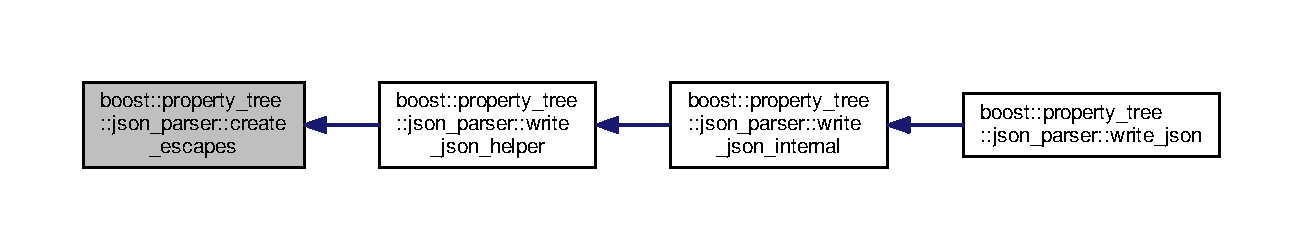
\includegraphics[width=350pt]{namespaceboost_1_1property__tree_1_1json__parser_a747e92e137769eb6b27edb76d613f37a_icgraph}
\end{center}
\end{figure}


\hypertarget{namespaceboost_1_1property__tree_1_1json__parser_a7aed126d35d2893e51c49399ba33c51e}{\index{boost\-::property\-\_\-tree\-::json\-\_\-parser@{boost\-::property\-\_\-tree\-::json\-\_\-parser}!read\-\_\-json@{read\-\_\-json}}
\index{read\-\_\-json@{read\-\_\-json}!boost::property_tree::json_parser@{boost\-::property\-\_\-tree\-::json\-\_\-parser}}
\subsubsection[{read\-\_\-json}]{\setlength{\rightskip}{0pt plus 5cm}template$<$class Ptree $>$ void boost\-::property\-\_\-tree\-::json\-\_\-parser\-::read\-\_\-json (
\begin{DoxyParamCaption}
\item[{std\-::basic\-\_\-istream$<$ typename Ptree\-::key\-\_\-type\-::value\-\_\-type $>$ \&}]{stream, }
\item[{Ptree \&}]{pt}
\end{DoxyParamCaption}
)}}\label{namespaceboost_1_1property__tree_1_1json__parser_a7aed126d35d2893e51c49399ba33c51e}
Read J\-S\-O\-N from a the given stream and translate it to a property tree. \begin{DoxyNote}{Note}
Clears existing contents of property tree. In case of error the property tree unmodified. 

Items of J\-S\-O\-N arrays are translated into ptree keys with empty names. Members of objects are translated into named keys. 

J\-S\-O\-N data can be a string, a numeric value, or one of literals \char`\"{}null\char`\"{}, \char`\"{}true\char`\"{} and \char`\"{}false\char`\"{}. During parse, any of the above is copied verbatim into ptree data string. 
\end{DoxyNote}

\begin{DoxyExceptions}{Exceptions}
{\em json\-\_\-parser\-\_\-error} & In case of error deserializing the property tree. \\
\hline
\end{DoxyExceptions}

\begin{DoxyParams}[1]{Parameters}
 & {\em stream} & Stream from which to read in the property tree. \\
\hline
\mbox{\tt out}  & {\em pt} & The property tree to populate. \\
\hline
\end{DoxyParams}


Definition at line 98 of file json\-\_\-parser.\-hpp.


\begin{DoxyCode}
102 \{
103   read\_json\_internal(stream, pt, std::string());
104 \}
\end{DoxyCode}
\hypertarget{namespaceboost_1_1property__tree_1_1json__parser_aa8344dc0b7987cba89b0630195d7a34d}{\index{boost\-::property\-\_\-tree\-::json\-\_\-parser@{boost\-::property\-\_\-tree\-::json\-\_\-parser}!read\-\_\-json@{read\-\_\-json}}
\index{read\-\_\-json@{read\-\_\-json}!boost::property_tree::json_parser@{boost\-::property\-\_\-tree\-::json\-\_\-parser}}
\subsubsection[{read\-\_\-json}]{\setlength{\rightskip}{0pt plus 5cm}template$<$class Ptree $>$ void boost\-::property\-\_\-tree\-::json\-\_\-parser\-::read\-\_\-json (
\begin{DoxyParamCaption}
\item[{const std\-::string \&}]{filename, }
\item[{Ptree \&}]{pt, }
\item[{const std\-::locale \&}]{loc = {\ttfamily std\-:\-:locale()}}
\end{DoxyParamCaption}
)}}\label{namespaceboost_1_1property__tree_1_1json__parser_aa8344dc0b7987cba89b0630195d7a34d}
Read J\-S\-O\-N from a the given file and translate it to a property tree. \begin{DoxyNote}{Note}
Clears existing contents of property tree. In case of error the property tree unmodified. 

Items of J\-S\-O\-N arrays are translated into ptree keys with empty names. Members of objects are translated into named keys. 

J\-S\-O\-N data can be a string, a numeric value, or one of literals \char`\"{}null\char`\"{}, \char`\"{}true\char`\"{} and \char`\"{}false\char`\"{}. During parse, any of the above is copied verbatim into ptree data string. 
\end{DoxyNote}

\begin{DoxyExceptions}{Exceptions}
{\em json\-\_\-parser\-\_\-error} & In case of error deserializing the property tree. \\
\hline
\end{DoxyExceptions}

\begin{DoxyParams}[1]{Parameters}
 & {\em filename} & Name of file from which to read in the property tree. \\
\hline
\mbox{\tt out}  & {\em pt} & The property tree to populate. \\
\hline
 & {\em loc} & The locale to use when reading in the file contents. \\
\hline
\end{DoxyParams}


Definition at line 122 of file json\-\_\-parser.\-hpp.


\begin{DoxyCode}
125 \{
126   std::basic\_ifstream<typename Ptree::key\_type::value\_type>
127     stream(filename.c\_str());
128   \textcolor{keywordflow}{if} (!stream)
129     BOOST\_PROPERTY\_TREE\_THROW(json\_parser\_error(
130                                                 \textcolor{stringliteral}{"cannot open file"}, filename, 0));
131   stream.imbue(loc);
132   read\_json\_internal(stream, pt, filename);
133 \}
\end{DoxyCode}
\hypertarget{namespaceboost_1_1property__tree_1_1json__parser_ad1f43753e8e91845fdb1177c1aa0c465}{\index{boost\-::property\-\_\-tree\-::json\-\_\-parser@{boost\-::property\-\_\-tree\-::json\-\_\-parser}!verify\-\_\-json@{verify\-\_\-json}}
\index{verify\-\_\-json@{verify\-\_\-json}!boost::property_tree::json_parser@{boost\-::property\-\_\-tree\-::json\-\_\-parser}}
\subsubsection[{verify\-\_\-json}]{\setlength{\rightskip}{0pt plus 5cm}template$<$class Ptree $>$ bool boost\-::property\-\_\-tree\-::json\-\_\-parser\-::verify\-\_\-json (
\begin{DoxyParamCaption}
\item[{const Ptree \&}]{pt, }
\item[{int}]{depth}
\end{DoxyParamCaption}
)}}\label{namespaceboost_1_1property__tree_1_1json__parser_ad1f43753e8e91845fdb1177c1aa0c465}


Definition at line 138 of file json\-\_\-parser\-\_\-write.\-hpp.


\begin{DoxyCode}
139 \{
140 
141   \textcolor{keyword}{typedef} \textcolor{keyword}{typename} Ptree::key\_type::value\_type Ch;
142   \textcolor{keyword}{typedef} \textcolor{keyword}{typename} std::basic\_string<Ch> Str;
143 
144   \textcolor{comment}{// Root ptree cannot have data}
145   \textcolor{keywordflow}{if} (depth == 0 && !pt.template get\_value<Str>().empty())
146     \textcolor{keywordflow}{return} \textcolor{keyword}{false};
147 
148   \textcolor{comment}{// Ptree cannot have both children and data}
149   \textcolor{keywordflow}{if} (!pt.template get\_value<Str>().empty() && !pt.empty())
150     \textcolor{keywordflow}{return} \textcolor{keyword}{false};
151 
152   \textcolor{comment}{// Check children}
153   \textcolor{keyword}{typename} Ptree::const\_iterator it = pt.begin();
154   \textcolor{keywordflow}{for} (; it != pt.end(); ++it)
155     \textcolor{keywordflow}{if} (!\hyperlink{namespaceboost_1_1property__tree_1_1json__parser_ad1f43753e8e91845fdb1177c1aa0c465}{verify\_json}(it->second, depth + 1))
156       \textcolor{keywordflow}{return} \textcolor{keyword}{false};
157 
158   \textcolor{comment}{// Success}
159   \textcolor{keywordflow}{return} \textcolor{keyword}{true};
160 
161 \}
\end{DoxyCode}


Here is the caller graph for this function\-:
\nopagebreak
\begin{figure}[H]
\begin{center}
\leavevmode
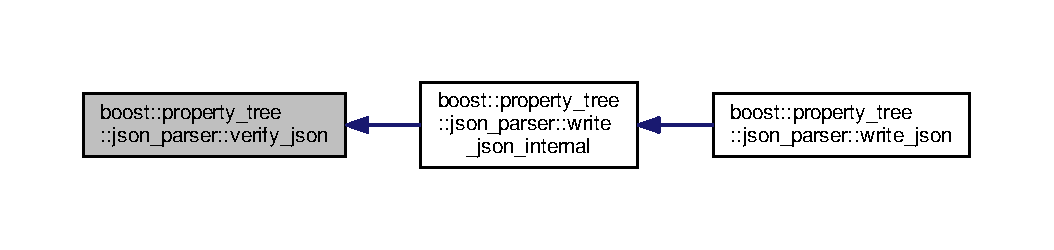
\includegraphics[width=350pt]{namespaceboost_1_1property__tree_1_1json__parser_ad1f43753e8e91845fdb1177c1aa0c465_icgraph}
\end{center}
\end{figure}


\hypertarget{namespaceboost_1_1property__tree_1_1json__parser_ad290247428581132003df8706e3ef9d0}{\index{boost\-::property\-\_\-tree\-::json\-\_\-parser@{boost\-::property\-\_\-tree\-::json\-\_\-parser}!write\-\_\-json@{write\-\_\-json}}
\index{write\-\_\-json@{write\-\_\-json}!boost::property_tree::json_parser@{boost\-::property\-\_\-tree\-::json\-\_\-parser}}
\subsubsection[{write\-\_\-json}]{\setlength{\rightskip}{0pt plus 5cm}template$<$class Ptree $>$ void boost\-::property\-\_\-tree\-::json\-\_\-parser\-::write\-\_\-json (
\begin{DoxyParamCaption}
\item[{std\-::basic\-\_\-ostream$<$ typename Ptree\-::key\-\_\-type\-::value\-\_\-type $>$ \&}]{stream, }
\item[{const Ptree \&}]{pt, }
\item[{bool}]{pretty = {\ttfamily true}}
\end{DoxyParamCaption}
)}}\label{namespaceboost_1_1property__tree_1_1json__parser_ad290247428581132003df8706e3ef9d0}
Translates the property tree to J\-S\-O\-N and writes it the given output stream. \begin{DoxyNote}{Note}
Any property tree key containing only unnamed subkeys will be rendered as J\-S\-O\-N arrays. 
\end{DoxyNote}
\begin{DoxyPrecond}{Precondition}
{\itshape pt} cannot contain keys that have both subkeys and non-\/empty data. 
\end{DoxyPrecond}

\begin{DoxyExceptions}{Exceptions}
{\em json\-\_\-parser\-\_\-error} & In case of error translating the property tree to J\-S\-O\-N or writing to the output stream. \\
\hline
\end{DoxyExceptions}

\begin{DoxyParams}{Parameters}
{\em stream} & The stream to which to write the J\-S\-O\-N representation of the property tree. \\
\hline
{\em pt} & The property tree to tranlsate to J\-S\-O\-N and output. \\
\hline
{\em pretty} & Whether to pretty-\/print. Defaults to true for backward compatibility. \\
\hline
\end{DoxyParams}


Definition at line 150 of file json\-\_\-parser.\-hpp.


\begin{DoxyCode}
155 \{
156   \hyperlink{namespaceboost_1_1property__tree_1_1json__parser_af1059520397d396ae91e776391a2f32b}{write\_json\_internal}(stream, pt, std::string(), pretty);
157 \}
\end{DoxyCode}


Here is the call graph for this function\-:
\nopagebreak
\begin{figure}[H]
\begin{center}
\leavevmode
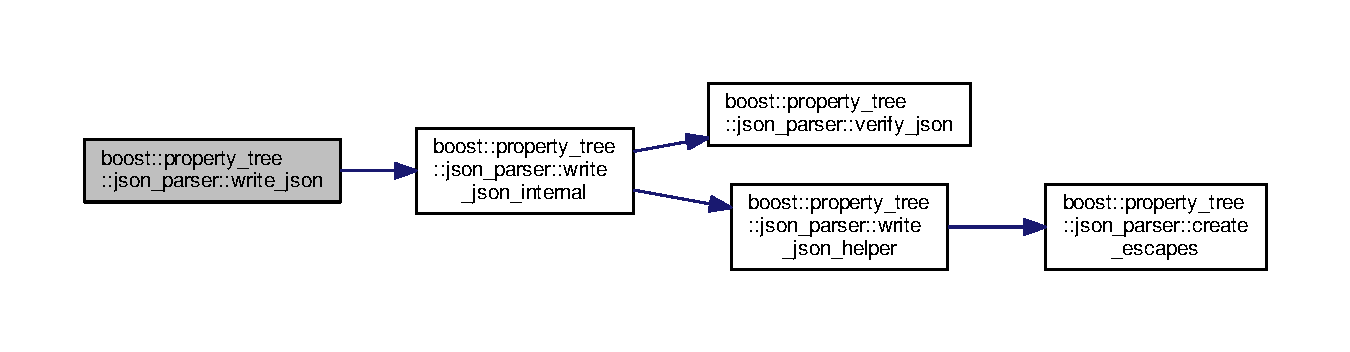
\includegraphics[width=350pt]{namespaceboost_1_1property__tree_1_1json__parser_ad290247428581132003df8706e3ef9d0_cgraph}
\end{center}
\end{figure}


\hypertarget{namespaceboost_1_1property__tree_1_1json__parser_a49f6a7c920e5ac943603a5f10ccf3a32}{\index{boost\-::property\-\_\-tree\-::json\-\_\-parser@{boost\-::property\-\_\-tree\-::json\-\_\-parser}!write\-\_\-json@{write\-\_\-json}}
\index{write\-\_\-json@{write\-\_\-json}!boost::property_tree::json_parser@{boost\-::property\-\_\-tree\-::json\-\_\-parser}}
\subsubsection[{write\-\_\-json}]{\setlength{\rightskip}{0pt plus 5cm}template$<$class Ptree $>$ void boost\-::property\-\_\-tree\-::json\-\_\-parser\-::write\-\_\-json (
\begin{DoxyParamCaption}
\item[{const std\-::string \&}]{filename, }
\item[{const Ptree \&}]{pt, }
\item[{const std\-::locale \&}]{loc = {\ttfamily std\-:\-:locale()}, }
\item[{bool}]{pretty = {\ttfamily true}}
\end{DoxyParamCaption}
)}}\label{namespaceboost_1_1property__tree_1_1json__parser_a49f6a7c920e5ac943603a5f10ccf3a32}
Translates the property tree to J\-S\-O\-N and writes it the given file. \begin{DoxyNote}{Note}
Any property tree key containing only unnamed subkeys will be rendered as J\-S\-O\-N arrays. 
\end{DoxyNote}
\begin{DoxyPrecond}{Precondition}
{\itshape pt} cannot contain keys that have both subkeys and non-\/empty data. 
\end{DoxyPrecond}

\begin{DoxyExceptions}{Exceptions}
{\em json\-\_\-parser\-\_\-error} & In case of error translating the property tree to J\-S\-O\-N or writing to the file. \\
\hline
\end{DoxyExceptions}

\begin{DoxyParams}{Parameters}
{\em filename} & The name of the file to which to write the J\-S\-O\-N representation of the property tree. \\
\hline
{\em pt} & The property tree to translate to J\-S\-O\-N and output. \\
\hline
{\em loc} & The locale to use when writing out to the output file. \\
\hline
{\em pretty} & Whether to pretty-\/print. Defaults to true and last place for backward compatibility. \\
\hline
\end{DoxyParams}


Definition at line 174 of file json\-\_\-parser.\-hpp.


\begin{DoxyCode}
178 \{
179   std::basic\_ofstream<typename Ptree::key\_type::value\_type>
180     stream(filename.c\_str());
181   \textcolor{keywordflow}{if} (!stream)
182     BOOST\_PROPERTY\_TREE\_THROW(json\_parser\_error(
183                                                 \textcolor{stringliteral}{"cannot open file"}, filename, 0));
184   stream.imbue(loc);
185   \hyperlink{namespaceboost_1_1property__tree_1_1json__parser_af1059520397d396ae91e776391a2f32b}{write\_json\_internal}(stream, pt, filename, pretty);
186 \}
\end{DoxyCode}


Here is the call graph for this function\-:
\nopagebreak
\begin{figure}[H]
\begin{center}
\leavevmode
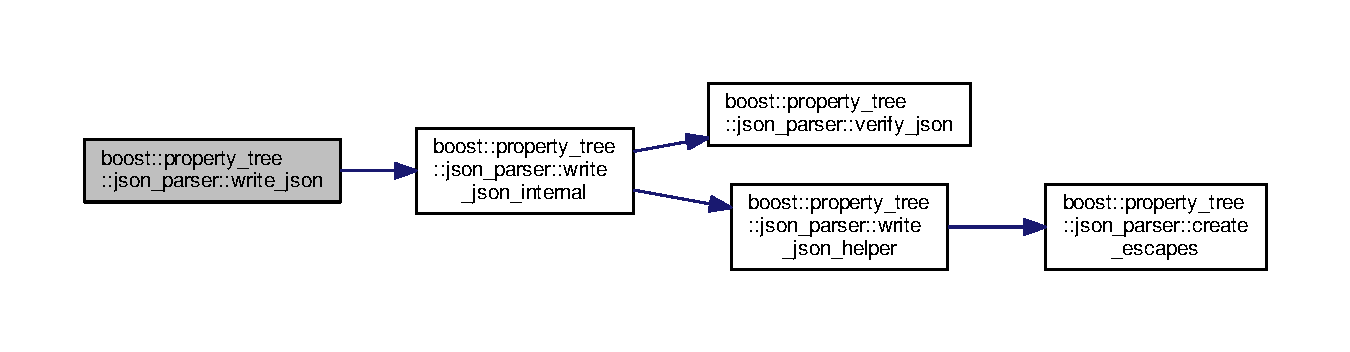
\includegraphics[width=350pt]{namespaceboost_1_1property__tree_1_1json__parser_a49f6a7c920e5ac943603a5f10ccf3a32_cgraph}
\end{center}
\end{figure}


\hypertarget{namespaceboost_1_1property__tree_1_1json__parser_a133973ddea67e6d77424312cd297b332}{\index{boost\-::property\-\_\-tree\-::json\-\_\-parser@{boost\-::property\-\_\-tree\-::json\-\_\-parser}!write\-\_\-json\-\_\-helper@{write\-\_\-json\-\_\-helper}}
\index{write\-\_\-json\-\_\-helper@{write\-\_\-json\-\_\-helper}!boost::property_tree::json_parser@{boost\-::property\-\_\-tree\-::json\-\_\-parser}}
\subsubsection[{write\-\_\-json\-\_\-helper}]{\setlength{\rightskip}{0pt plus 5cm}template$<$class Ptree $>$ void boost\-::property\-\_\-tree\-::json\-\_\-parser\-::write\-\_\-json\-\_\-helper (
\begin{DoxyParamCaption}
\item[{std\-::basic\-\_\-ostream$<$ typename Ptree\-::key\-\_\-type\-::value\-\_\-type $>$ \&}]{stream, }
\item[{const Ptree \&}]{pt, }
\item[{int}]{indent, }
\item[{bool}]{pretty}
\end{DoxyParamCaption}
)}}\label{namespaceboost_1_1property__tree_1_1json__parser_a133973ddea67e6d77424312cd297b332}


Definition at line 76 of file json\-\_\-parser\-\_\-write.\-hpp.


\begin{DoxyCode}
79 \{
80 
81   \textcolor{keyword}{typedef} \textcolor{keyword}{typename} Ptree::key\_type::value\_type Ch;
82   \textcolor{keyword}{typedef} \textcolor{keyword}{typename} std::basic\_string<Ch> Str;
83 
84   \textcolor{comment}{// Value or object or array}
85   \textcolor{keywordflow}{if} (indent > 0 && pt.empty())
86   \{
87     \textcolor{comment}{// Write value}
88     Str data = \hyperlink{namespaceboost_1_1property__tree_1_1json__parser_a747e92e137769eb6b27edb76d613f37a}{create\_escapes}(pt.template get\_value<Str>());
89     stream << data;
90 
91   \}
92   \textcolor{keywordflow}{else} \textcolor{keywordflow}{if} (indent > 0 && pt.count(Str()) == pt.size())
93   \{
94     \textcolor{comment}{// Write array}
95     stream << Ch(\textcolor{charliteral}{'['});
96     \textcolor{keywordflow}{if} (pretty) stream << Ch(\textcolor{charliteral}{'\(\backslash\)n'});
97     \textcolor{keyword}{typename} Ptree::const\_iterator it = pt.begin();
98     \textcolor{keywordflow}{for} (; it != pt.end(); ++it)
99     \{
100       \textcolor{keywordflow}{if} (pretty) stream << Str(4 * (indent + 1), Ch(\textcolor{charliteral}{' '}));
101       \hyperlink{namespaceboost_1_1property__tree_1_1json__parser_a133973ddea67e6d77424312cd297b332}{write\_json\_helper}(stream, it->second, indent + 1, pretty);
102       \textcolor{keywordflow}{if} (boost::next(it) != pt.end())
103         stream << Ch(\textcolor{charliteral}{','});
104       \textcolor{keywordflow}{if} (pretty) stream << Ch(\textcolor{charliteral}{'\(\backslash\)n'});
105     \}
106     stream << Str(4 * indent, Ch(\textcolor{charliteral}{' '})) << Ch(\textcolor{charliteral}{']'});
107 
108   \}
109   \textcolor{keywordflow}{else}
110   \{
111     \textcolor{comment}{// Write object}
112     stream << Ch(\textcolor{charliteral}{'\{'});
113     \textcolor{keywordflow}{if} (pretty) stream << Ch(\textcolor{charliteral}{'\(\backslash\)n'});
114     \textcolor{keyword}{typename} Ptree::const\_iterator it = pt.begin();
115     \textcolor{keywordflow}{for} (; it != pt.end(); ++it)
116     \{
117       \textcolor{keywordflow}{if} (pretty) stream << Str(4 * (indent + 1), Ch(\textcolor{charliteral}{' '}));
118       stream << Ch(\textcolor{charliteral}{'"'}) << \hyperlink{namespaceboost_1_1property__tree_1_1json__parser_a747e92e137769eb6b27edb76d613f37a}{create\_escapes}(it->first) << Ch(\textcolor{charliteral}{'"'}) << Ch(\textcolor{charliteral}{':'});
119       \textcolor{keywordflow}{if} (pretty) \{
120         \textcolor{keywordflow}{if} (it->second.empty())
121           stream << Ch(\textcolor{charliteral}{' '});
122         \textcolor{keywordflow}{else}
123           stream << Ch(\textcolor{charliteral}{'\(\backslash\)n'}) << Str(4 * (indent + 1), Ch(\textcolor{charliteral}{' '}));
124       \}
125       \hyperlink{namespaceboost_1_1property__tree_1_1json__parser_a133973ddea67e6d77424312cd297b332}{write\_json\_helper}(stream, it->second, indent + 1, pretty);
126       \textcolor{keywordflow}{if} (boost::next(it) != pt.end())
127         stream << Ch(\textcolor{charliteral}{','});
128       \textcolor{keywordflow}{if} (pretty) stream << Ch(\textcolor{charliteral}{'\(\backslash\)n'});
129     \}
130     \textcolor{keywordflow}{if} (pretty) stream << Str(4 * indent, Ch(\textcolor{charliteral}{' '}));
131     stream << Ch(\textcolor{charliteral}{'\}'});
132   \}
133 
134 \}
\end{DoxyCode}


Here is the call graph for this function\-:
\nopagebreak
\begin{figure}[H]
\begin{center}
\leavevmode
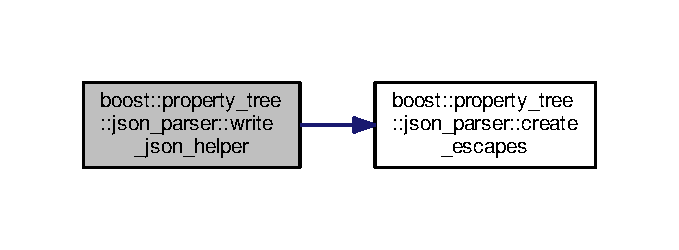
\includegraphics[width=326pt]{namespaceboost_1_1property__tree_1_1json__parser_a133973ddea67e6d77424312cd297b332_cgraph}
\end{center}
\end{figure}




Here is the caller graph for this function\-:
\nopagebreak
\begin{figure}[H]
\begin{center}
\leavevmode
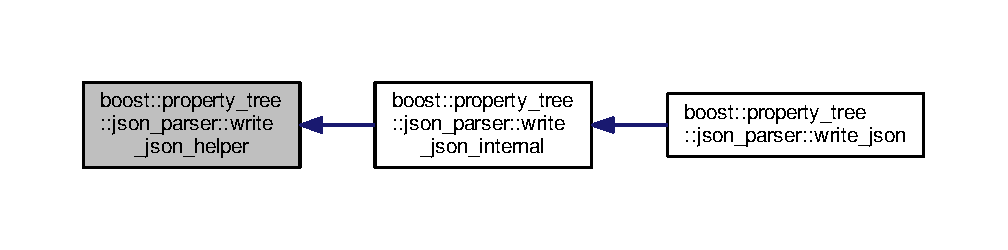
\includegraphics[width=350pt]{namespaceboost_1_1property__tree_1_1json__parser_a133973ddea67e6d77424312cd297b332_icgraph}
\end{center}
\end{figure}


\hypertarget{namespaceboost_1_1property__tree_1_1json__parser_af1059520397d396ae91e776391a2f32b}{\index{boost\-::property\-\_\-tree\-::json\-\_\-parser@{boost\-::property\-\_\-tree\-::json\-\_\-parser}!write\-\_\-json\-\_\-internal@{write\-\_\-json\-\_\-internal}}
\index{write\-\_\-json\-\_\-internal@{write\-\_\-json\-\_\-internal}!boost::property_tree::json_parser@{boost\-::property\-\_\-tree\-::json\-\_\-parser}}
\subsubsection[{write\-\_\-json\-\_\-internal}]{\setlength{\rightskip}{0pt plus 5cm}template$<$class Ptree $>$ void boost\-::property\-\_\-tree\-::json\-\_\-parser\-::write\-\_\-json\-\_\-internal (
\begin{DoxyParamCaption}
\item[{std\-::basic\-\_\-ostream$<$ typename Ptree\-::key\-\_\-type\-::value\-\_\-type $>$ \&}]{stream, }
\item[{const Ptree \&}]{pt, }
\item[{const std\-::string \&}]{filename, }
\item[{bool}]{pretty}
\end{DoxyParamCaption}
)}}\label{namespaceboost_1_1property__tree_1_1json__parser_af1059520397d396ae91e776391a2f32b}


Definition at line 165 of file json\-\_\-parser\-\_\-write.\-hpp.


\begin{DoxyCode}
169 \{
170   \textcolor{keywordflow}{if} (!\hyperlink{namespaceboost_1_1property__tree_1_1json__parser_ad1f43753e8e91845fdb1177c1aa0c465}{verify\_json}(pt, 0))
171     BOOST\_PROPERTY\_TREE\_THROW(json\_parser\_error(\textcolor{stringliteral}{"ptree contains data that cannot be represented in JSON
       format"}, filename, 0));
172   \hyperlink{namespaceboost_1_1property__tree_1_1json__parser_a133973ddea67e6d77424312cd297b332}{write\_json\_helper}(stream, pt, 0, pretty);
173   stream << std::endl;
174   \textcolor{keywordflow}{if} (!stream.good())
175     BOOST\_PROPERTY\_TREE\_THROW(json\_parser\_error(\textcolor{stringliteral}{"write error"}, filename, 0));
176 \}
\end{DoxyCode}


Here is the call graph for this function\-:
\nopagebreak
\begin{figure}[H]
\begin{center}
\leavevmode
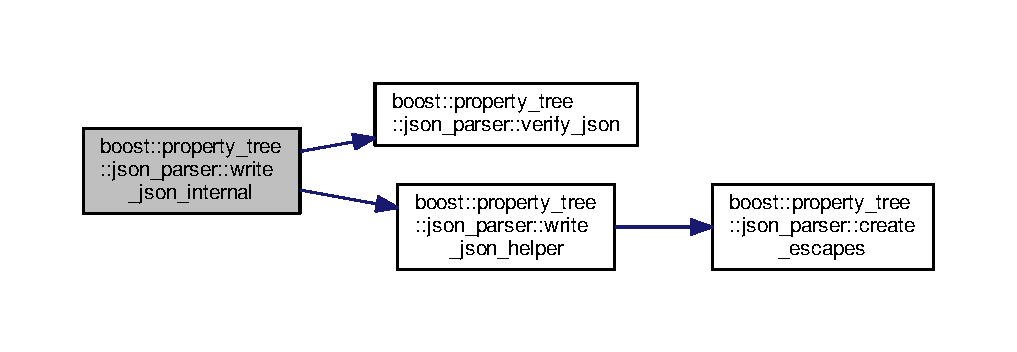
\includegraphics[width=350pt]{namespaceboost_1_1property__tree_1_1json__parser_af1059520397d396ae91e776391a2f32b_cgraph}
\end{center}
\end{figure}




Here is the caller graph for this function\-:
\nopagebreak
\begin{figure}[H]
\begin{center}
\leavevmode
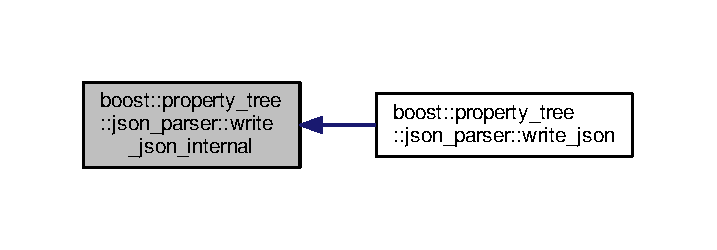
\includegraphics[width=344pt]{namespaceboost_1_1property__tree_1_1json__parser_af1059520397d396ae91e776391a2f32b_icgraph}
\end{center}
\end{figure}



\hypertarget{namespacextd}{\section{xtd Namespace Reference}
\label{namespacextd}\index{xtd@{xtd}}
}
\subsection*{Namespaces}
\begin{DoxyCompactItemize}
\item 
\hyperlink{namespacextd_1_1text}{text}
\end{DoxyCompactItemize}
\subsection*{Classes}
\begin{DoxyCompactItemize}
\item 
class \hyperlink{classxtd_1_1Application}{Application}
\begin{DoxyCompactList}\small\item\em Parses arguments from \hyperlink{doc_2example_2Application_8hh_a6b77b2233054447db17959182b5fb02b}{main(int,char$\ast$$\ast$)} function. \end{DoxyCompactList}\item 
class \hyperlink{classxtd_1_1ConfParser}{Conf\-Parser}
\item 
class \hyperlink{classxtd_1_1error}{error}
\item 
class \hyperlink{classxtd_1_1logger}{logger}
\end{DoxyCompactItemize}
\subsection*{Enumerations}
\begin{DoxyCompactItemize}
\item 
enum \hyperlink{namespacextd_a68ed4fe8e9c11116b68efe5b102aec50}{status} \-: uint32\-\_\-t \{ \hyperlink{namespacextd_a68ed4fe8e9c11116b68efe5b102aec50a444bcb3a3fcf8389296c49467f27e1d6}{status\-::ok} = 0, 
\hyperlink{namespacextd_a68ed4fe8e9c11116b68efe5b102aec50acb5e100e5a9a3e7f6d1fd97512215282}{status\-::error} = 1, 
\hyperlink{namespacextd_a68ed4fe8e9c11116b68efe5b102aec50a90272dda245ae1fb3cf197e91a8689dc}{status\-::timeout} = 2, 
\hyperlink{namespacextd_a68ed4fe8e9c11116b68efe5b102aec50ac2adf6ecc220f2711801d6e466340183}{status\-::notfound} = 3
 \}
\end{DoxyCompactItemize}
\subsection*{Functions}
\begin{DoxyCompactItemize}
\item 
{\footnotesize template$<$typename T $>$ }\\std\-::underlying\-\_\-type$<$ T $>$\-::type \hyperlink{namespacextd_a518b0ddcbf87f6c21175d2760f4fbe21}{valueof} (T p\-\_\-item)
\end{DoxyCompactItemize}


\subsection{Enumeration Type Documentation}
\hypertarget{namespacextd_a68ed4fe8e9c11116b68efe5b102aec50}{\index{xtd@{xtd}!status@{status}}
\index{status@{status}!xtd@{xtd}}
\subsubsection[{status}]{\setlength{\rightskip}{0pt plus 5cm}enum {\bf xtd\-::status} \-: uint32\-\_\-t\hspace{0.3cm}{\ttfamily [strong]}}}\label{namespacextd_a68ed4fe8e9c11116b68efe5b102aec50}
\begin{Desc}
\item[Enumerator]\par
\begin{description}
\index{ok@{ok}!xtd@{xtd}}\index{xtd@{xtd}!ok@{ok}}\item[{\em 
\hypertarget{namespacextd_a68ed4fe8e9c11116b68efe5b102aec50a444bcb3a3fcf8389296c49467f27e1d6}{ok}\label{namespacextd_a68ed4fe8e9c11116b68efe5b102aec50a444bcb3a3fcf8389296c49467f27e1d6}
}]\index{error@{error}!xtd@{xtd}}\index{xtd@{xtd}!error@{error}}\item[{\em 
\hypertarget{namespacextd_a68ed4fe8e9c11116b68efe5b102aec50acb5e100e5a9a3e7f6d1fd97512215282}{error}\label{namespacextd_a68ed4fe8e9c11116b68efe5b102aec50acb5e100e5a9a3e7f6d1fd97512215282}
}]\index{timeout@{timeout}!xtd@{xtd}}\index{xtd@{xtd}!timeout@{timeout}}\item[{\em 
\hypertarget{namespacextd_a68ed4fe8e9c11116b68efe5b102aec50a90272dda245ae1fb3cf197e91a8689dc}{timeout}\label{namespacextd_a68ed4fe8e9c11116b68efe5b102aec50a90272dda245ae1fb3cf197e91a8689dc}
}]\index{notfound@{notfound}!xtd@{xtd}}\index{xtd@{xtd}!notfound@{notfound}}\item[{\em 
\hypertarget{namespacextd_a68ed4fe8e9c11116b68efe5b102aec50ac2adf6ecc220f2711801d6e466340183}{notfound}\label{namespacextd_a68ed4fe8e9c11116b68efe5b102aec50ac2adf6ecc220f2711801d6e466340183}
}]\end{description}
\end{Desc}


Definition at line 37 of file types.\-hh.


\begin{DoxyCode}
37 : uint32\_t \{ \hyperlink{namespacextd_a68ed4fe8e9c11116b68efe5b102aec50a444bcb3a3fcf8389296c49467f27e1d6}{ok} = 0, \hyperlink{namespacextd_a68ed4fe8e9c11116b68efe5b102aec50acb5e100e5a9a3e7f6d1fd97512215282}{error} = 1, \hyperlink{namespacextd_a68ed4fe8e9c11116b68efe5b102aec50a90272dda245ae1fb3cf197e91a8689dc}{timeout} = 2, \hyperlink{namespacextd_a68ed4fe8e9c11116b68efe5b102aec50ac2adf6ecc220f2711801d6e466340183}{notfound} = 3 \};
\end{DoxyCode}


\subsection{Function Documentation}
\hypertarget{namespacextd_a518b0ddcbf87f6c21175d2760f4fbe21}{\index{xtd@{xtd}!valueof@{valueof}}
\index{valueof@{valueof}!xtd@{xtd}}
\subsubsection[{valueof}]{\setlength{\rightskip}{0pt plus 5cm}template$<$typename T $>$ std\-::underlying\-\_\-type$<$T$>$\-::type xtd\-::valueof (
\begin{DoxyParamCaption}
\item[{T}]{p\-\_\-item}
\end{DoxyParamCaption}
)}}\label{namespacextd_a518b0ddcbf87f6c21175d2760f4fbe21}


Definition at line 32 of file types.\-hh.


\begin{DoxyCode}
33 \{
34   \textcolor{keywordflow}{return} \textcolor{keyword}{static\_cast<}typename std::underlying\_type<T>::type\textcolor{keyword}{>}(p\_item);
35 \}
\end{DoxyCode}

\hypertarget{namespacextd_1_1text}{}\section{xtd\+:\+:text Namespace Reference}
\label{namespacextd_1_1text}\index{xtd\+::text@{xtd\+::text}}
\subsection*{Classes}
\begin{DoxyCompactItemize}
\item 
class \hyperlink{classxtd_1_1text_1_1xml}{xml}
\end{DoxyCompactItemize}

\chapter{Class Documentation}
\hypertarget{classApp}{\section{App Class Reference}
\label{classApp}\index{App@{App}}
}


Inheritance diagram for App\-:
\nopagebreak
\begin{figure}[H]
\begin{center}
\leavevmode
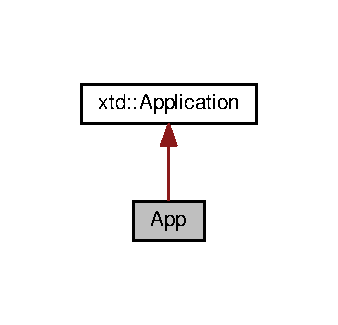
\includegraphics[width=162pt]{classApp__inherit__graph}
\end{center}
\end{figure}


Collaboration diagram for App\-:
\nopagebreak
\begin{figure}[H]
\begin{center}
\leavevmode
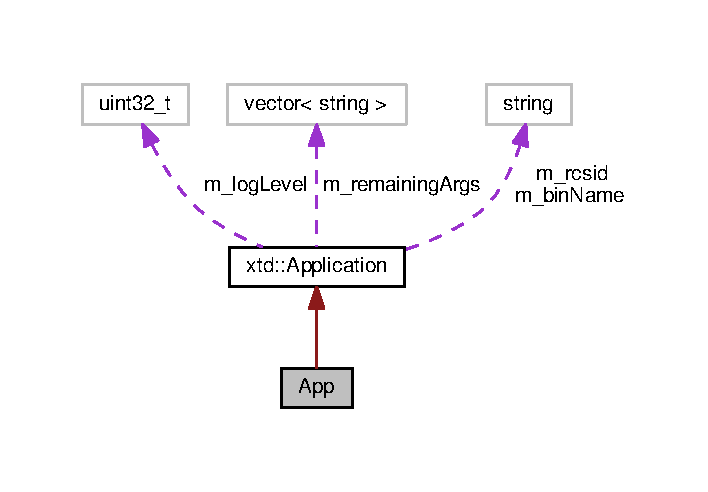
\includegraphics[width=340pt]{classApp__coll__graph}
\end{center}
\end{figure}


\subsection{Detailed Description}


Definition at line 7 of file main.\-cc.



The documentation for this class was generated from the following file\-:\begin{DoxyCompactItemize}
\item 
/home/travis/build/psycofdj/xtdcpp/common/src/\hyperlink{main_8cc}{main.\-cc}\end{DoxyCompactItemize}

\hypertarget{classxtd_1_1Application}{}\section{xtd\+:\+:Application Class Reference}
\label{classxtd_1_1Application}\index{xtd\+::\+Application@{xtd\+::\+Application}}


Parses arguments from \hyperlink{doc_2example_2Application_8hh_a6b77b2233054447db17959182b5fb02b}{main(int,char$\ast$$\ast$)} function.  




{\ttfamily \#include $<$Application.\+hh$>$}



Inheritance diagram for xtd\+:\+:Application\+:
\nopagebreak
\begin{figure}[H]
\begin{center}
\leavevmode
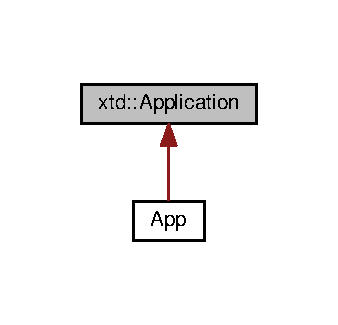
\includegraphics[width=164pt]{classxtd_1_1Application__inherit__graph}
\end{center}
\end{figure}


Collaboration diagram for xtd\+:\+:Application\+:
\nopagebreak
\begin{figure}[H]
\begin{center}
\leavevmode
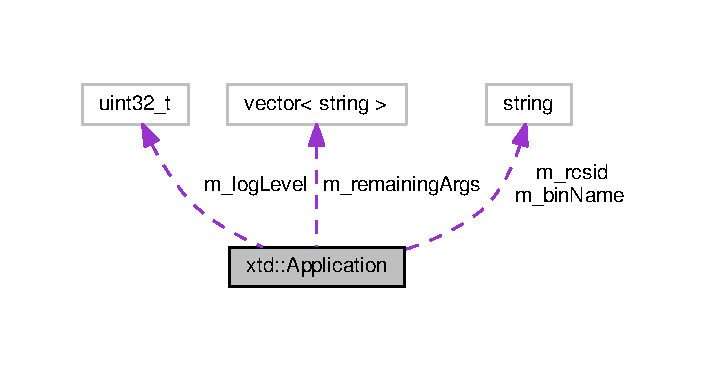
\includegraphics[width=341pt]{classxtd_1_1Application__coll__graph}
\end{center}
\end{figure}
\subsection*{Public Member Functions}
\begin{DoxyCompactItemize}
\item 
\hyperlink{classxtd_1_1Application_a2d911d40f42dc2928275538541b91633}{Application} (void)
\begin{DoxyCompactList}\small\item\em Constructor. \end{DoxyCompactList}\item 
virtual \hyperlink{classxtd_1_1Application_a3ae7e81534c6ca594339e3e098183df4}{$\sim$\+Application} (void)
\begin{DoxyCompactList}\small\item\em Destructor. \end{DoxyCompactList}\item 
int \hyperlink{classxtd_1_1Application_ae9241351a9caefa4b96bc906d3db144c}{execute} (int p\+\_\+argc, char $\ast$$\ast$p\+\_\+argv)
\begin{DoxyCompactList}\small\item\em main entry point, usually called with \hyperlink{doc_2example_2Application_8hh_a6b77b2233054447db17959182b5fb02b}{main(int,char$\ast$$\ast$)}\textquotesingle{}s arguments \end{DoxyCompactList}\end{DoxyCompactItemize}
\subsection*{Protected Types}
\begin{DoxyCompactItemize}
\item 
enum \hyperlink{classxtd_1_1Application_a672c075ed901e463609077d571a714c7}{argument} \+: uint32\+\_\+t \{ \hyperlink{classxtd_1_1Application_a672c075ed901e463609077d571a714c7ad57c24f3fe52d16e7169b912dd647f0d}{argument\+::optional} = 0, 
\hyperlink{classxtd_1_1Application_a672c075ed901e463609077d571a714c7ac5e3b9675d114c21ad3367d318f6aa95}{argument\+::mandatory} = 1, 
\hyperlink{classxtd_1_1Application_a672c075ed901e463609077d571a714c7a334c4a4c42fdb79d7ebc3e73b517e6f8}{argument\+::none} = 2
 \}\begin{DoxyCompactList}\small\item\em Behavior switch for the argument of an option. \end{DoxyCompactList}
\item 
enum \hyperlink{classxtd_1_1Application_a49c0397e9fd22067e3a536443a17fe24}{requirement} \+: uint32\+\_\+t \{ \hyperlink{classxtd_1_1Application_a49c0397e9fd22067e3a536443a17fe24ad57c24f3fe52d16e7169b912dd647f0d}{requirement\+::optional} = 0, 
\hyperlink{classxtd_1_1Application_a49c0397e9fd22067e3a536443a17fe24ac5e3b9675d114c21ad3367d318f6aa95}{requirement\+::mandatory} = 1
 \}\begin{DoxyCompactList}\small\item\em Behavior for the presence of the option itself. \end{DoxyCompactList}
\item 
typedef std\+::function$<$ void(void)$>$ \hyperlink{classxtd_1_1Application_a907b6fe8247636495890e668530863d6}{t\+\_\+sig\+\_\+handler}
\end{DoxyCompactItemize}
\subsection*{Protected Member Functions}
\begin{DoxyCompactItemize}
\item 
virtual void \hyperlink{classxtd_1_1Application_a8684d1d061027893f91580106a821d88}{parse\+Config} (void)
\begin{DoxyCompactList}\small\item\em Parse application configuration, (default nothing) \end{DoxyCompactList}\item 
virtual void \hyperlink{classxtd_1_1Application_a3c63f070ac7baaea43a32b3064d0030b}{check\+Options} (void)
\begin{DoxyCompactList}\small\item\em Check read options, (default nothing) \end{DoxyCompactList}\item 
virtual void \hyperlink{classxtd_1_1Application_ab8e835ba678494c42e12c4613958d18a}{initialize} (void)
\begin{DoxyCompactList}\small\item\em initialize application, (default nothing) \end{DoxyCompactList}\item 
virtual int \hyperlink{classxtd_1_1Application_aef6043d47982bc1983a84e2c8a53f0cd}{process} (void)
\begin{DoxyCompactList}\small\item\em Main application process function, (default nothing) \end{DoxyCompactList}\item 
bool \hyperlink{classxtd_1_1Application_afdb5173d0105fcf549ee6f61e6dcbe49}{add\+Signal\+Handler} (int p\+\_\+signal\+Number, \hyperlink{classxtd_1_1Application_a907b6fe8247636495890e668530863d6}{t\+\_\+sig\+\_\+handler} p\+\_\+handler)
\begin{DoxyCompactList}\small\item\em register a signal callback \end{DoxyCompactList}\item 
const string \& \hyperlink{classxtd_1_1Application_ab7be8fa583daa66271562a83817b172c}{get\+Version} (void) const 
\begin{DoxyCompactList}\small\item\em Get R\+C\+S\+ID identity informations. \end{DoxyCompactList}\item 
void \hyperlink{classxtd_1_1Application_a7cea42a03984ceed3bae129ff9e1ef54}{add\+Option} (const char p\+\_\+short\+Opt, const string \&p\+\_\+long\+Opt, const \hyperlink{classxtd_1_1Application_a672c075ed901e463609077d571a714c7}{argument} p\+\_\+arg\+Type, const \hyperlink{classxtd_1_1Application_a49c0397e9fd22067e3a536443a17fe24}{requirement} p\+\_\+status, const string \&p\+\_\+description, t\+\_\+callback p\+\_\+callback)
\item 
bool \hyperlink{classxtd_1_1Application_a4aca412c4a0bcd761e28b0350bd71578}{is\+Option\+Given} (const string \&p\+\_\+option\+Name) const 
\begin{DoxyCompactList}\small\item\em Tells if given option was given on command line. \end{DoxyCompactList}\item 
void \hyperlink{classxtd_1_1Application_abdfaafd220104a063c344a4f7e126ec0}{add\+Help\+Msg} (const string \&p\+\_\+help\+Message)
\begin{DoxyCompactList}\small\item\em Add additional usage line to display on help or errors. \end{DoxyCompactList}\item 
t\+\_\+callback \hyperlink{classxtd_1_1Application_a2b491ba745bbd3b2d01d9e623c0aff60}{bind\+Dir} (string \&p\+\_\+target, bool p\+\_\+readable=true) const 
\begin{DoxyCompactList}\small\item\em Bind option\textquotesingle{}s parameter to a directory. \end{DoxyCompactList}\item 
t\+\_\+callback \hyperlink{classxtd_1_1Application_ab10f6dde0bf4034dff7eafe8a45c2029}{bind\+File} (string \&p\+\_\+target, bool p\+\_\+readable=true) const 
\begin{DoxyCompactList}\small\item\em Bind option\textquotesingle{}s parameter to a file name. \end{DoxyCompactList}\item 
t\+\_\+callback \hyperlink{classxtd_1_1Application_a59b986c85c2e1d9473f73df10425dfcf}{bind\+Given} (bool \&p\+\_\+target) const 
\begin{DoxyCompactList}\small\item\em Set targeted variable to true if option is given on command line. \end{DoxyCompactList}\item 
t\+\_\+callback \hyperlink{classxtd_1_1Application_a36a351db3830e2e894a39fbd42842280}{bind\+String} (string \&p\+\_\+target) const 
\begin{DoxyCompactList}\small\item\em Set targeted variable to option\textquotesingle{}s parameter. \end{DoxyCompactList}\item 
{\footnotesize template$<$typename T $>$ }\\t\+\_\+callback \hyperlink{classxtd_1_1Application_a00f6aed6c376028a79492b04e8325968}{bind\+Callback} (T p\+\_\+action) const 
\begin{DoxyCompactList}\small\item\em Associate option to given generic callback. \end{DoxyCompactList}\item 
{\footnotesize template$<$typename T $>$ }\\t\+\_\+callback \hyperlink{classxtd_1_1Application_a2415acb66badb368e726173fb884097c}{bind\+Value\+If\+Given} (T \&p\+\_\+target, const T \&p\+\_\+value) const 
\begin{DoxyCompactList}\small\item\em Set given value to referenced variable if option is given. \end{DoxyCompactList}\item 
{\footnotesize template$<$typename T $>$ }\\t\+\_\+callback \hyperlink{classxtd_1_1Application_ae5fd6c9b1d2ad5225f9d624f63df4173}{bind\+Number} (T \&p\+\_\+target, T p\+\_\+min=std\+::numeric\+\_\+limits$<$ T $>$\+::min(), T p\+\_\+max=std\+::numeric\+\_\+limits$<$ T $>$\+::max()) const 
\begin{DoxyCompactList}\small\item\em Bind option\textquotesingle{}s paramter as number to referenced variable. \end{DoxyCompactList}\item 
{\footnotesize template$<$typename T , class Iterable $>$ }\\t\+\_\+callback \hyperlink{classxtd_1_1Application_aaa0388f1c96893a26cfe5522b0804dd9}{bind\+Values} (T \&p\+\_\+target, const Iterable \&p\+\_\+values) const 
\begin{DoxyCompactList}\small\item\em Bind option\textquotesingle{}s parameter to target variable and checks among authorized values. \end{DoxyCompactList}\item 
{\footnotesize template$<$typename T , template$<$ class $>$ class T\+Collection$>$ }\\t\+\_\+callback \hyperlink{classxtd_1_1Application_a846da30aaf55754027608ddf5c689366}{bind\+Accumulator} (T\+Collection$<$ T $>$ \&p\+\_\+target) const 
\begin{DoxyCompactList}\small\item\em Append option\textquotesingle{}s parameter to target container for each command line hit. \end{DoxyCompactList}\item 
{\footnotesize template$<$typename... Arguments$>$ }\\void \hyperlink{classxtd_1_1Application_a810c6c1924f762fd453555cb91cb35f9}{error\+\_\+nohelp} (int p\+\_\+code, const string \&p\+\_\+format, Arguments \&\&...p\+\_\+args) const 
\begin{DoxyCompactList}\small\item\em Prints error on standard error and exit. \end{DoxyCompactList}\item 
{\footnotesize template$<$typename... Arguments$>$ }\\void \hyperlink{classxtd_1_1Application_adf84f52f1388bef1336d0fb5f6345563}{error} (int p\+\_\+code, const string \&p\+\_\+format, Arguments \&\&...p\+\_\+args) const 
\begin{DoxyCompactList}\small\item\em Prints error and usage on standard error and exit. \end{DoxyCompactList}\item 
{\footnotesize template$<$typename... Arguments$>$ }\\void \hyperlink{classxtd_1_1Application_a931877468f6b948909d596d91d60b7a2}{warn} (const string \&p\+\_\+format, Arguments \&\&...p\+\_\+args) const 
\begin{DoxyCompactList}\small\item\em Prints a warning on standard error. \end{DoxyCompactList}\end{DoxyCompactItemize}
\subsection*{Protected Attributes}
\begin{DoxyCompactItemize}
\item 
string \hyperlink{classxtd_1_1Application_abdf4c6f863c5a7a4ee842906f546c458}{m\+\_\+bin\+Name}
\begin{DoxyCompactList}\small\item\em binary name (argv\mbox{[}0\mbox{]}) \end{DoxyCompactList}\item 
uint32\+\_\+t \hyperlink{classxtd_1_1Application_a3f815061d81aa12974b2b6ee48b9f5e9}{m\+\_\+log\+Level}
\begin{DoxyCompactList}\small\item\em log level read from command line \end{DoxyCompactList}\item 
vector$<$ string $>$ \hyperlink{classxtd_1_1Application_a7651fd3849530cdded556187a6b42c25}{m\+\_\+remaining\+Args}
\begin{DoxyCompactList}\small\item\em positional command line arguments \end{DoxyCompactList}\item 
string \hyperlink{classxtd_1_1Application_ad820953bc15b729ce010f422595d3a3f}{m\+\_\+rcsid}
\begin{DoxyCompactList}\small\item\em binary identity information \end{DoxyCompactList}\end{DoxyCompactItemize}


\subsection{Detailed Description}
Parses arguments from \hyperlink{doc_2example_2Application_8hh_a6b77b2233054447db17959182b5fb02b}{main(int,char$\ast$$\ast$)} function. 


\begin{DoxyItemize}
\item \hyperlink{classxtd_1_1Application_sec_intro}{Introcution}
\item \hyperlink{classxtd_1_1Application_sec_howto}{How to use}
\item \hyperlink{classxtd_1_1Application_sec_execution_flow}{Execution flow}
\item \hyperlink{classxtd_1_1Application_sec_binding_options}{Bindind options}
\end{DoxyItemize}\hypertarget{classxtd_1_1Application_sec_intro}{}\subsection{Introcution}\label{classxtd_1_1Application_sec_intro}
This object provides a default application skeleton including \+:
\begin{DoxyItemize}
\item user-\/friendly wrapping of argument parsing (on top of C\textquotesingle{}s getopt\+\_\+long)
\item usage generator for declared options
\item default options \+: --help and --log-\/level
\item default logging facility
\item signal handling on a separate thread
\item binary R\+CS identity tracking, usually generated by xtd compile-\/time dependency tracking system
\end{DoxyItemize}\hypertarget{classxtd_1_1Application_sec_howto}{}\subsection{How to use}\label{classxtd_1_1Application_sec_howto}

\begin{DoxyEnumerate}
\item Inherit your class from \hyperlink{classxtd_1_1Application}{Application}
\item Define the mandatory method \hyperlink{classxtd_1_1Application_aef6043d47982bc1983a84e2c8a53f0cd}{Application\+::process}
\item Declare your program arguments in your constructor
\item Optionaly parse your configuration, check your parameters and initialize your application in the dedicated methods
\item Instantiate your class in \hyperlink{doc_2example_2Application_8hh_a6b77b2233054447db17959182b5fb02b}{main(int,char$\ast$$\ast$)} function and all \hyperlink{classxtd_1_1Application_ae9241351a9caefa4b96bc906d3db144c}{Application\+::execute} method
\end{DoxyEnumerate}

Typical example \+: 
\begin{DoxyCodeInclude}
\textcolor{keyword}{class }\hyperlink{classMyApp}{MyApp} : \textcolor{keyword}{public} \hyperlink{classxtd_1_1Application_a2d911d40f42dc2928275538541b91633}{Application}
 \{
 \textcolor{keyword}{public}:
   \hyperlink{classMyApp}{MyApp}(\textcolor{keywordtype}{void}) :
     \hyperlink{classxtd_1_1Application_a2d911d40f42dc2928275538541b91633}{Application}()
   \{
     \hyperlink{classxtd_1_1Application_a7cea42a03984ceed3bae129ff9e1ef54}{addOption}(\textcolor{charliteral}{'i'}, \textcolor{stringliteral}{"input-file"},
               \hyperlink{classxtd_1_1Application_a672c075ed901e463609077d571a714c7ac5e3b9675d114c21ad3367d318f6aa95}{argument::mandatory},
               \hyperlink{classxtd_1_1Application_a49c0397e9fd22067e3a536443a17fe24ac5e3b9675d114c21ad3367d318f6aa95}{requirement::mandatory},
               \textcolor{stringliteral}{"process given file"},
               \hyperlink{classxtd_1_1Application_ab10f6dde0bf4034dff7eafe8a45c2029}{Application::bindFile}(m\_inputFile, \textcolor{keyword}{true}));
   \}

 \textcolor{keyword}{private}:
   \textcolor{keywordtype}{int} \hyperlink{classxtd_1_1Application_aef6043d47982bc1983a84e2c8a53f0cd}{process}(\textcolor{keywordtype}{void})
   \{
     std::cout << \textcolor{stringliteral}{"given readable file : "} << m\_inputFile << std::endl;

     \textcolor{comment}{// do some stuff}
     \textcolor{keywordflow}{return} (l\_success) ? 0 : 1;
   \}

 \textcolor{keyword}{private}:
   std::string m\_inputFile;
\};


\textcolor{keywordtype}{int} \hyperlink{main_8cc_af847876e048f60529674b0f221f6edc1}{main}(\textcolor{keywordtype}{int} p\_argc, \textcolor{keywordtype}{char}** p\_argv)
\{
  \hyperlink{classMyApp}{MyApp} l\_app;
  \textcolor{keywordflow}{return} l\_app.execute(p\_argc, p\_argv);
\}
\end{DoxyCodeInclude}
\hypertarget{classxtd_1_1Application_sec_execution_flow}{}\subsection{Execution flow}\label{classxtd_1_1Application_sec_execution_flow}

\begin{DoxyImageNoCaption}
  \mbox{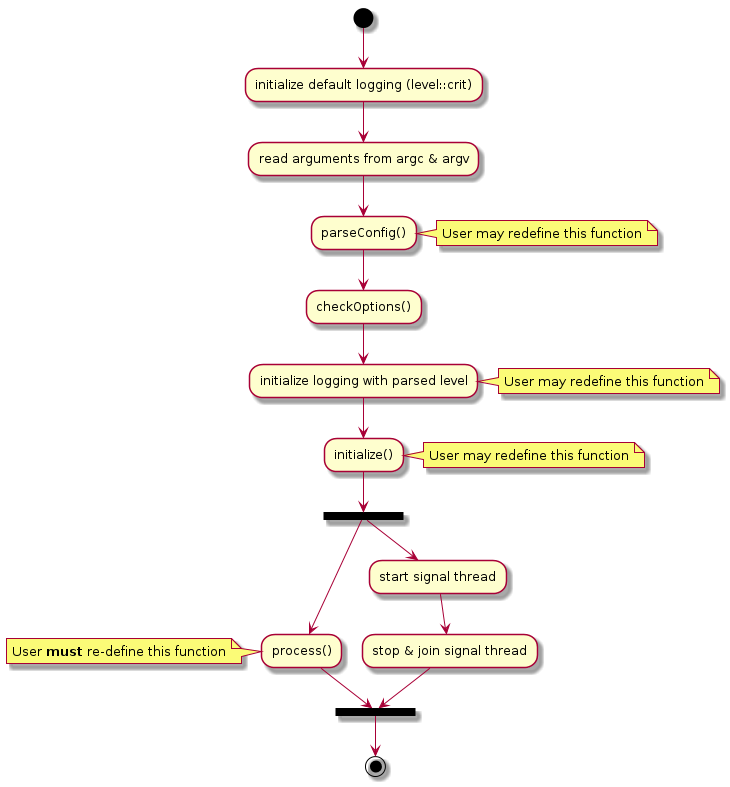
\includegraphics[width=\textwidth,height=\textheight/2,keepaspectratio=true]{Application}}
\end{DoxyImageNoCaption}
\hypertarget{classxtd_1_1Application_sec_binding_options}{}\subsection{Bindind options}\label{classxtd_1_1Application_sec_binding_options}

\begin{DoxyItemize}
\item \hyperlink{classxtd_1_1Application_a2b491ba745bbd3b2d01d9e623c0aff60}{bind\+Dir} \+: Bind option\textquotesingle{}s parameter to a directory.
\item \hyperlink{classxtd_1_1Application_ab10f6dde0bf4034dff7eafe8a45c2029}{bind\+File} \+: Bind option\textquotesingle{}s parameter to a file name.
\item \hyperlink{classxtd_1_1Application_a59b986c85c2e1d9473f73df10425dfcf}{bind\+Given} \+: Set targeted variable to true if option is given on command line.
\item \hyperlink{classxtd_1_1Application_a36a351db3830e2e894a39fbd42842280}{bind\+String} \+: Set targeted variable to option\textquotesingle{}s parameter.
\item \hyperlink{classxtd_1_1Application_a00f6aed6c376028a79492b04e8325968}{bind\+Callback} \+: Associate option to given generic callback.
\item \hyperlink{classxtd_1_1Application_a2415acb66badb368e726173fb884097c}{bind\+Value\+If\+Given} \+: Set given value to referenced variable if option is given.
\item \hyperlink{classxtd_1_1Application_ae5fd6c9b1d2ad5225f9d624f63df4173}{bind\+Number} \+: Bind option\textquotesingle{}s paramter as number to referenced variable.
\item \hyperlink{classxtd_1_1Application_aaa0388f1c96893a26cfe5522b0804dd9}{bind\+Values} \+: Bind option\textquotesingle{}s parameter to target variable and checks among authorized values.
\item \hyperlink{classxtd_1_1Application_a846da30aaf55754027608ddf5c689366}{bind\+Accumulator} \+: Append option\textquotesingle{}s parameter to target container for each command line hit. 
\end{DoxyItemize}

Definition at line 86 of file Application.\+hh.



\subsection{Member Typedef Documentation}
\index{xtd\+::\+Application@{xtd\+::\+Application}!t\+\_\+sig\+\_\+handler@{t\+\_\+sig\+\_\+handler}}
\index{t\+\_\+sig\+\_\+handler@{t\+\_\+sig\+\_\+handler}!xtd\+::\+Application@{xtd\+::\+Application}}
\subsubsection[{\texorpdfstring{t\+\_\+sig\+\_\+handler}{t_sig_handler}}]{\setlength{\rightskip}{0pt plus 5cm}typedef std\+::function$<$void(void)$>$ {\bf xtd\+::\+Application\+::t\+\_\+sig\+\_\+handler}\hspace{0.3cm}{\ttfamily [protected]}}\hypertarget{classxtd_1_1Application_a907b6fe8247636495890e668530863d6}{}\label{classxtd_1_1Application_a907b6fe8247636495890e668530863d6}


Definition at line 89 of file Application.\+hh.



\subsection{Member Enumeration Documentation}
\index{xtd\+::\+Application@{xtd\+::\+Application}!argument@{argument}}
\index{argument@{argument}!xtd\+::\+Application@{xtd\+::\+Application}}
\subsubsection[{\texorpdfstring{argument}{argument}}]{\setlength{\rightskip}{0pt plus 5cm}enum {\bf xtd\+::\+Application\+::argument} \+: uint32\+\_\+t\hspace{0.3cm}{\ttfamily [strong]}, {\ttfamily [protected]}}\hypertarget{classxtd_1_1Application_a672c075ed901e463609077d571a714c7}{}\label{classxtd_1_1Application_a672c075ed901e463609077d571a714c7}


Behavior switch for the argument of an option. 

\begin{Desc}
\item[Enumerator]\par
\begin{description}
\index{optional@{optional}!xtd\+::\+Application@{xtd\+::\+Application}}\index{xtd\+::\+Application@{xtd\+::\+Application}!optional@{optional}}\item[{\em 
optional\hypertarget{classxtd_1_1Application_a672c075ed901e463609077d571a714c7ad57c24f3fe52d16e7169b912dd647f0d}{}\label{classxtd_1_1Application_a672c075ed901e463609077d571a714c7ad57c24f3fe52d16e7169b912dd647f0d}
}]optional argument for option \index{mandatory@{mandatory}!xtd\+::\+Application@{xtd\+::\+Application}}\index{xtd\+::\+Application@{xtd\+::\+Application}!mandatory@{mandatory}}\item[{\em 
mandatory\hypertarget{classxtd_1_1Application_a672c075ed901e463609077d571a714c7ac5e3b9675d114c21ad3367d318f6aa95}{}\label{classxtd_1_1Application_a672c075ed901e463609077d571a714c7ac5e3b9675d114c21ad3367d318f6aa95}
}]mandatory argument for option \index{none@{none}!xtd\+::\+Application@{xtd\+::\+Application}}\index{xtd\+::\+Application@{xtd\+::\+Application}!none@{none}}\item[{\em 
none\hypertarget{classxtd_1_1Application_a672c075ed901e463609077d571a714c7a334c4a4c42fdb79d7ebc3e73b517e6f8}{}\label{classxtd_1_1Application_a672c075ed901e463609077d571a714c7a334c4a4c42fdb79d7ebc3e73b517e6f8}
}]forbidden argument for option \end{description}
\end{Desc}


Definition at line 95 of file Application.\+hh.


\begin{DoxyCode}
95                       : uint32\_t
96   \{
97     optional  = 0, 
98     mandatory = 1, 
99     none      = 2  
100   \};
\end{DoxyCode}
\index{xtd\+::\+Application@{xtd\+::\+Application}!requirement@{requirement}}
\index{requirement@{requirement}!xtd\+::\+Application@{xtd\+::\+Application}}
\subsubsection[{\texorpdfstring{requirement}{requirement}}]{\setlength{\rightskip}{0pt plus 5cm}enum {\bf xtd\+::\+Application\+::requirement} \+: uint32\+\_\+t\hspace{0.3cm}{\ttfamily [strong]}, {\ttfamily [protected]}}\hypertarget{classxtd_1_1Application_a49c0397e9fd22067e3a536443a17fe24}{}\label{classxtd_1_1Application_a49c0397e9fd22067e3a536443a17fe24}


Behavior for the presence of the option itself. 

\begin{Desc}
\item[Enumerator]\par
\begin{description}
\index{optional@{optional}!xtd\+::\+Application@{xtd\+::\+Application}}\index{xtd\+::\+Application@{xtd\+::\+Application}!optional@{optional}}\item[{\em 
optional\hypertarget{classxtd_1_1Application_a49c0397e9fd22067e3a536443a17fe24ad57c24f3fe52d16e7169b912dd647f0d}{}\label{classxtd_1_1Application_a49c0397e9fd22067e3a536443a17fe24ad57c24f3fe52d16e7169b912dd647f0d}
}]option is optional on command line \index{mandatory@{mandatory}!xtd\+::\+Application@{xtd\+::\+Application}}\index{xtd\+::\+Application@{xtd\+::\+Application}!mandatory@{mandatory}}\item[{\em 
mandatory\hypertarget{classxtd_1_1Application_a49c0397e9fd22067e3a536443a17fe24ac5e3b9675d114c21ad3367d318f6aa95}{}\label{classxtd_1_1Application_a49c0397e9fd22067e3a536443a17fe24ac5e3b9675d114c21ad3367d318f6aa95}
}]option must be given on command line \end{description}
\end{Desc}


Definition at line 106 of file Application.\+hh.


\begin{DoxyCode}
106                          : uint32\_t
107   \{
108     optional  = 0, 
109     mandatory = 1  
110   \};
\end{DoxyCode}


\subsection{Constructor \& Destructor Documentation}
\index{xtd\+::\+Application@{xtd\+::\+Application}!Application@{Application}}
\index{Application@{Application}!xtd\+::\+Application@{xtd\+::\+Application}}
\subsubsection[{\texorpdfstring{Application(void)}{Application(void)}}]{\setlength{\rightskip}{0pt plus 5cm}Application\+::\+Application (
\begin{DoxyParamCaption}
\item[{void}]{}
\end{DoxyParamCaption}
)}\hypertarget{classxtd_1_1Application_a2d911d40f42dc2928275538541b91633}{}\label{classxtd_1_1Application_a2d911d40f42dc2928275538541b91633}


Constructor. 



Definition at line 20 of file Application.\+cc.


\begin{DoxyCode}
20                              :
21   \hyperlink{classxtd_1_1Application_abdf4c6f863c5a7a4ee842906f546c458}{m\_binName}(),
22   \hyperlink{classxtd_1_1Application_a3f815061d81aa12974b2b6ee48b9f5e9}{m\_logLevel}(\hyperlink{classxtd_1_1logger_a21511dfdad9ec1e88c3444637a000e9d}{logger::get}().valueOf(\hyperlink{classxtd_1_1logger_a250ce2f143da181d7149a1556da2a6f1a5888c6a8bb862595985926d16c7dcf13}{logger::level::crit})),
23   \hyperlink{classxtd_1_1Application_a7651fd3849530cdded556187a6b42c25}{m\_remainingArgs}(),
24   \hyperlink{classxtd_1_1Application_ad820953bc15b729ce010f422595d3a3f}{m\_rcsid}(\hyperlink{Application_8cc_a69f59503b72db9ae6ac36f5f5deaeb80}{rcsid}),
25   m\_optionList(),
26   m\_helpText(),
27   m\_runThread(),
28   m\_work(m\_ioService),
29   m\_signals(m\_ioService),
30   m\_signalHandlerMap()
31 \{
32   \hyperlink{classxtd_1_1Application_a7cea42a03984ceed3bae129ff9e1ef54}{addOption}(\textcolor{charliteral}{'h'}, \textcolor{stringliteral}{"help"},
33             \hyperlink{classxtd_1_1Application_a672c075ed901e463609077d571a714c7a334c4a4c42fdb79d7ebc3e73b517e6f8}{argument::none},
34             \hyperlink{classxtd_1_1Application_a49c0397e9fd22067e3a536443a17fe24ad57c24f3fe52d16e7169b912dd647f0d}{requirement::optional},
35             \textcolor{stringliteral}{"imprime ce message"},
36             \hyperlink{classxtd_1_1Application_a00f6aed6c376028a79492b04e8325968}{bindCallback}(std::bind(&Application::usageWrapper, \textcolor{keyword}{this})));
37 
38   \hyperlink{classxtd_1_1Application_a7cea42a03984ceed3bae129ff9e1ef54}{addOption}(\textcolor{charliteral}{'e'}, \textcolor{stringliteral}{"log-level"},
39             \hyperlink{classxtd_1_1Application_a672c075ed901e463609077d571a714c7ac5e3b9675d114c21ad3367d318f6aa95}{argument::mandatory},
40             \hyperlink{classxtd_1_1Application_a49c0397e9fd22067e3a536443a17fe24ad57c24f3fe52d16e7169b912dd647f0d}{requirement::optional},
41             \textcolor{stringliteral}{"change le niveau de log à <arg> (defaut 2)"},
42             \hyperlink{classxtd_1_1Application_aaa0388f1c96893a26cfe5522b0804dd9}{bindValues}(\hyperlink{classxtd_1_1Application_a3f815061d81aa12974b2b6ee48b9f5e9}{m\_logLevel}, vector<uint32\_t>(\{0u, 1u, 2u, 3u, 4u, 5u, 6u, 7u\})))
      ;
43 
44   m\_signals.async\_wait(std::bind(&Application::handleSignal, \textcolor{keyword}{this}, std::placeholders::\_1, 
      std::placeholders::\_2));
45 \}
\end{DoxyCode}


Here is the call graph for this function\+:
\nopagebreak
\begin{figure}[H]
\begin{center}
\leavevmode
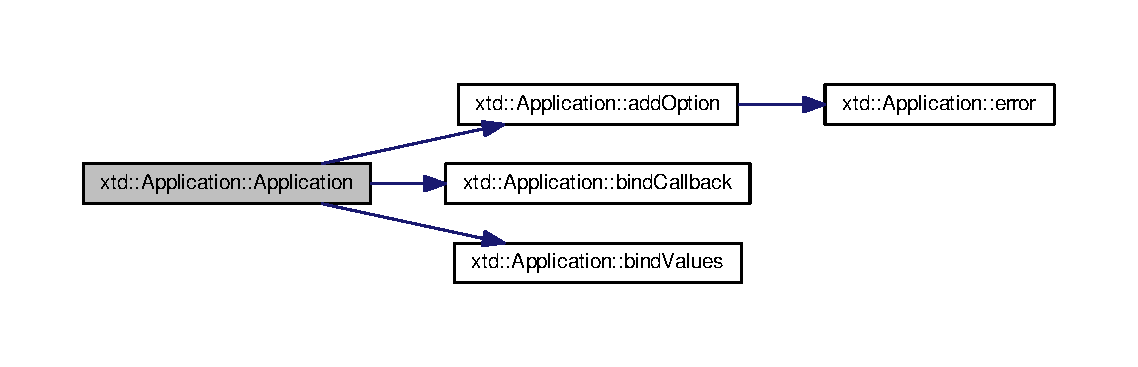
\includegraphics[width=350pt]{classxtd_1_1Application_a2d911d40f42dc2928275538541b91633_cgraph}
\end{center}
\end{figure}


\index{xtd\+::\+Application@{xtd\+::\+Application}!````~Application@{$\sim$\+Application}}
\index{````~Application@{$\sim$\+Application}!xtd\+::\+Application@{xtd\+::\+Application}}
\subsubsection[{\texorpdfstring{$\sim$\+Application(void)}{~Application(void)}}]{\setlength{\rightskip}{0pt plus 5cm}Application\+::$\sim$\+Application (
\begin{DoxyParamCaption}
\item[{void}]{}
\end{DoxyParamCaption}
)\hspace{0.3cm}{\ttfamily [virtual]}}\hypertarget{classxtd_1_1Application_a3ae7e81534c6ca594339e3e098183df4}{}\label{classxtd_1_1Application_a3ae7e81534c6ca594339e3e098183df4}


Destructor. 



Definition at line 47 of file Application.\+cc.


\begin{DoxyCode}
48 \{
49 \}
\end{DoxyCode}


\subsection{Member Function Documentation}
\index{xtd\+::\+Application@{xtd\+::\+Application}!add\+Help\+Msg@{add\+Help\+Msg}}
\index{add\+Help\+Msg@{add\+Help\+Msg}!xtd\+::\+Application@{xtd\+::\+Application}}
\subsubsection[{\texorpdfstring{add\+Help\+Msg(const string \&p\+\_\+help\+Message)}{addHelpMsg(const string &p_helpMessage)}}]{\setlength{\rightskip}{0pt plus 5cm}void Application\+::add\+Help\+Msg (
\begin{DoxyParamCaption}
\item[{const string \&}]{p\+\_\+help\+Message}
\end{DoxyParamCaption}
)\hspace{0.3cm}{\ttfamily [protected]}}\hypertarget{classxtd_1_1Application_abdfaafd220104a063c344a4f7e126ec0}{}\label{classxtd_1_1Application_abdfaafd220104a063c344a4f7e126ec0}


Add additional usage line to display on help or errors. 


\begin{DoxyParams}{Parameters}
{\em p\+\_\+help\+Message} & Message line to add \\
\hline
\end{DoxyParams}


Definition at line 363 of file Application.\+cc.


\begin{DoxyCode}
364 \{
365   \textcolor{keywordflow}{if} (m\_helpText.size())
366     m\_helpText += \textcolor{stringliteral}{"\(\backslash\)n"};
367   m\_helpText += \textcolor{stringliteral}{"  "} + p\_helpMessage;
368 \}
\end{DoxyCode}


Here is the caller graph for this function\+:
\nopagebreak
\begin{figure}[H]
\begin{center}
\leavevmode
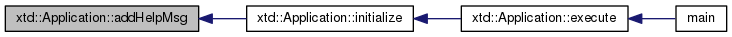
\includegraphics[width=350pt]{classxtd_1_1Application_abdfaafd220104a063c344a4f7e126ec0_icgraph}
\end{center}
\end{figure}


\index{xtd\+::\+Application@{xtd\+::\+Application}!add\+Option@{add\+Option}}
\index{add\+Option@{add\+Option}!xtd\+::\+Application@{xtd\+::\+Application}}
\subsubsection[{\texorpdfstring{add\+Option(const char p\+\_\+short\+Opt, const string \&p\+\_\+long\+Opt, const argument p\+\_\+arg\+Type, const requirement p\+\_\+status, const string \&p\+\_\+description, t\+\_\+callback p\+\_\+callback)}{addOption(const char p_shortOpt, const string &p_longOpt, const argument p_argType, const requirement p_status, const string &p_description, t_callback p_callback)}}]{\setlength{\rightskip}{0pt plus 5cm}void Application\+::add\+Option (
\begin{DoxyParamCaption}
\item[{const char}]{p\+\_\+short\+Opt, }
\item[{const string \&}]{p\+\_\+long\+Opt, }
\item[{const {\bf argument}}]{p\+\_\+arg\+Type, }
\item[{const {\bf requirement}}]{p\+\_\+status, }
\item[{const string \&}]{p\+\_\+description, }
\item[{t\+\_\+callback}]{p\+\_\+callback}
\end{DoxyParamCaption}
)\hspace{0.3cm}{\ttfamily [protected]}}\hypertarget{classxtd_1_1Application_a7cea42a03984ceed3bae129ff9e1ef54}{}\label{classxtd_1_1Application_a7cea42a03984ceed3bae129ff9e1ef54}


Definition at line 172 of file Application.\+cc.


\begin{DoxyCode}
178 \{
179   t\_option                l\_opt;
180 
181   \textcolor{keyword}{auto} l\_checker =
182     [\textcolor{keyword}{this}, p\_shortOpt, &p\_longOpt](\textcolor{keyword}{const} t\_option\_list::value\_type& c\_optItem) \{
183     \textcolor{keywordflow}{if} ((c\_optItem.m\_shortOpt == p\_shortOpt)                       ||
184         ((c\_optItem.m\_longOpt == p\_longOpt) && (p\_longOpt != \textcolor{stringliteral}{""})))
185     \{
186       \hyperlink{classxtd_1_1Application_adf84f52f1388bef1336d0fb5f6345563}{error}(1, \textcolor{stringliteral}{"short option '%c' already exists"}, p\_shortOpt);
187     \}
188   \};
189 
190   std::for\_each(m\_optionList.begin(), m\_optionList.end(), l\_checker);
191 
192   l\_opt.m\_given        = \textcolor{keyword}{false};
193   l\_opt.m\_shortOpt     = p\_shortOpt;
194   l\_opt.m\_longOpt      = p\_longOpt;
195   l\_opt.m\_argumentType = p\_argType;
196   l\_opt.m\_status       = p\_status;
197   l\_opt.m\_description  = p\_description;
198   l\_opt.m\_callback     = p\_callback;
199   m\_optionList.push\_back(l\_opt);
200 \}
\end{DoxyCode}


Here is the call graph for this function\+:
\nopagebreak
\begin{figure}[H]
\begin{center}
\leavevmode
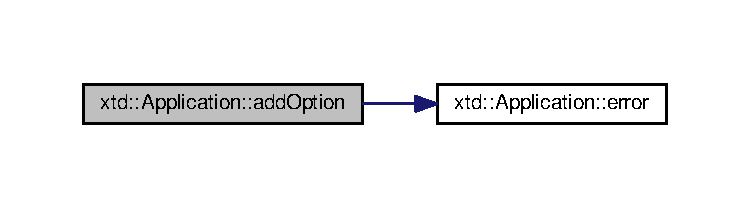
\includegraphics[width=350pt]{classxtd_1_1Application_a7cea42a03984ceed3bae129ff9e1ef54_cgraph}
\end{center}
\end{figure}




Here is the caller graph for this function\+:
\nopagebreak
\begin{figure}[H]
\begin{center}
\leavevmode
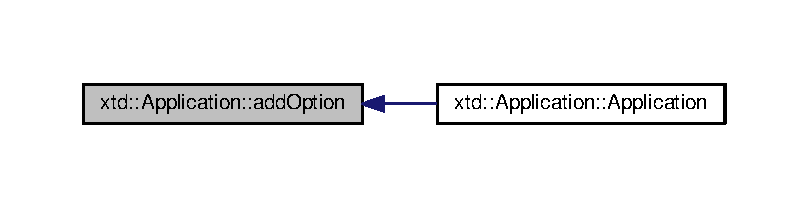
\includegraphics[width=350pt]{classxtd_1_1Application_a7cea42a03984ceed3bae129ff9e1ef54_icgraph}
\end{center}
\end{figure}


\index{xtd\+::\+Application@{xtd\+::\+Application}!add\+Signal\+Handler@{add\+Signal\+Handler}}
\index{add\+Signal\+Handler@{add\+Signal\+Handler}!xtd\+::\+Application@{xtd\+::\+Application}}
\subsubsection[{\texorpdfstring{add\+Signal\+Handler(int p\+\_\+signal\+Number, t\+\_\+sig\+\_\+handler p\+\_\+handler)}{addSignalHandler(int p_signalNumber, t_sig_handler p_handler)}}]{\setlength{\rightskip}{0pt plus 5cm}bool Application\+::add\+Signal\+Handler (
\begin{DoxyParamCaption}
\item[{int}]{p\+\_\+signal\+Number, }
\item[{{\bf t\+\_\+sig\+\_\+handler}}]{p\+\_\+handler}
\end{DoxyParamCaption}
)\hspace{0.3cm}{\ttfamily [protected]}}\hypertarget{classxtd_1_1Application_afdb5173d0105fcf549ee6f61e6dcbe49}{}\label{classxtd_1_1Application_afdb5173d0105fcf549ee6f61e6dcbe49}


register a signal callback 


\begin{DoxyParams}{Parameters}
{\em p\+\_\+signal\+Number} & signal ID (man signal 7) \\
\hline
{\em p\+\_\+handler} & handling callback \\
\hline
\end{DoxyParams}
\begin{DoxyReturn}{Returns}
True if signal registered correctly, false if signal was already registered 
\end{DoxyReturn}


Definition at line 155 of file Application.\+cc.


\begin{DoxyCode}
156 \{
157   \textcolor{keywordflow}{if} (m\_signalHandlerMap.find(p\_signalNumber) != m\_signalHandlerMap.end())
158     \textcolor{keywordflow}{return} \textcolor{keyword}{false};
159 
160   m\_signals.add(p\_signalNumber);
161   m\_signalHandlerMap[p\_signalNumber] = p\_handler;
162   \textcolor{keywordflow}{return} \textcolor{keyword}{true};
163 \}
\end{DoxyCode}


Here is the caller graph for this function\+:
\nopagebreak
\begin{figure}[H]
\begin{center}
\leavevmode
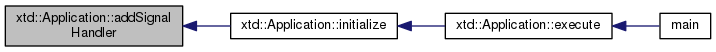
\includegraphics[width=350pt]{classxtd_1_1Application_afdb5173d0105fcf549ee6f61e6dcbe49_icgraph}
\end{center}
\end{figure}


\index{xtd\+::\+Application@{xtd\+::\+Application}!bind\+Accumulator@{bind\+Accumulator}}
\index{bind\+Accumulator@{bind\+Accumulator}!xtd\+::\+Application@{xtd\+::\+Application}}
\subsubsection[{\texorpdfstring{bind\+Accumulator(\+T\+Collection$<$ T $>$ \&p\+\_\+target) const }{bindAccumulator(TCollection< T > &p_target) const }}]{\setlength{\rightskip}{0pt plus 5cm}template$<$typename T , template$<$ class $>$ class T\+Collection$>$ t\+\_\+callback xtd\+::\+Application\+::bind\+Accumulator (
\begin{DoxyParamCaption}
\item[{T\+Collection$<$ T $>$ \&}]{p\+\_\+target}
\end{DoxyParamCaption}
) const\hspace{0.3cm}{\ttfamily [protected]}}\hypertarget{classxtd_1_1Application_a846da30aaf55754027608ddf5c689366}{}\label{classxtd_1_1Application_a846da30aaf55754027608ddf5c689366}


Append option\textquotesingle{}s parameter to target container for each command line hit. 


\begin{DoxyParams}{Parameters}
{\em p\+\_\+target} & Reference variable container \\
\hline
\end{DoxyParams}
\begin{DoxyReturn}{Returns}
generated option callback 
\end{DoxyReturn}


Here is the caller graph for this function\+:
\nopagebreak
\begin{figure}[H]
\begin{center}
\leavevmode
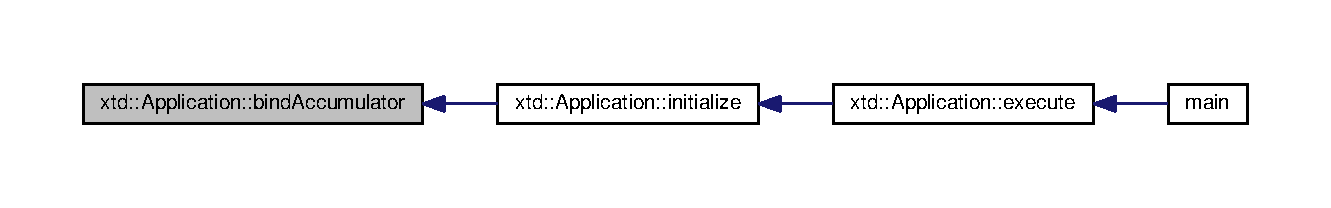
\includegraphics[width=350pt]{classxtd_1_1Application_a846da30aaf55754027608ddf5c689366_icgraph}
\end{center}
\end{figure}


\index{xtd\+::\+Application@{xtd\+::\+Application}!bind\+Callback@{bind\+Callback}}
\index{bind\+Callback@{bind\+Callback}!xtd\+::\+Application@{xtd\+::\+Application}}
\subsubsection[{\texorpdfstring{bind\+Callback(\+T p\+\_\+action) const }{bindCallback(T p_action) const }}]{\setlength{\rightskip}{0pt plus 5cm}template$<$typename T $>$ t\+\_\+callback xtd\+::\+Application\+::bind\+Callback (
\begin{DoxyParamCaption}
\item[{T}]{p\+\_\+action}
\end{DoxyParamCaption}
) const\hspace{0.3cm}{\ttfamily [protected]}}\hypertarget{classxtd_1_1Application_a00f6aed6c376028a79492b04e8325968}{}\label{classxtd_1_1Application_a00f6aed6c376028a79492b04e8325968}


Associate option to given generic callback. 


\begin{DoxyParams}{Parameters}
{\em p\+\_\+action} & function compatible with
\begin{DoxyCode}
std::function<void(void)> 
\end{DoxyCode}
 signature \\
\hline
\end{DoxyParams}
\begin{DoxyReturn}{Returns}
generated option callback 
\end{DoxyReturn}


Here is the caller graph for this function\+:
\nopagebreak
\begin{figure}[H]
\begin{center}
\leavevmode
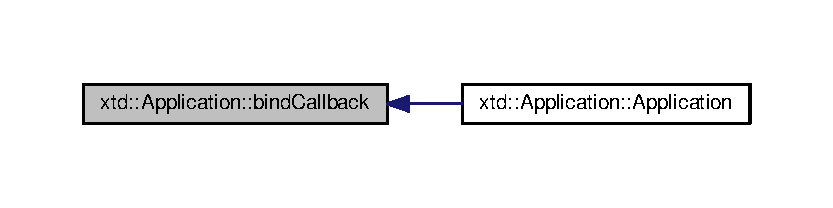
\includegraphics[width=350pt]{classxtd_1_1Application_a00f6aed6c376028a79492b04e8325968_icgraph}
\end{center}
\end{figure}


\index{xtd\+::\+Application@{xtd\+::\+Application}!bind\+Dir@{bind\+Dir}}
\index{bind\+Dir@{bind\+Dir}!xtd\+::\+Application@{xtd\+::\+Application}}
\subsubsection[{\texorpdfstring{bind\+Dir(string \&p\+\_\+target, bool p\+\_\+readable=true) const }{bindDir(string &p_target, bool p_readable=true) const }}]{\setlength{\rightskip}{0pt plus 5cm}Application\+::t\+\_\+callback Application\+::bind\+Dir (
\begin{DoxyParamCaption}
\item[{string \&}]{p\+\_\+target, }
\item[{bool}]{p\+\_\+readable = {\ttfamily true}}
\end{DoxyParamCaption}
) const\hspace{0.3cm}{\ttfamily [protected]}}\hypertarget{classxtd_1_1Application_a2b491ba745bbd3b2d01d9e623c0aff60}{}\label{classxtd_1_1Application_a2b491ba745bbd3b2d01d9e623c0aff60}


Bind option\textquotesingle{}s parameter to a directory. 


\begin{DoxyParams}{Parameters}
{\em p\+\_\+target} & Reference variable to store the option\textquotesingle{}s value \\
\hline
{\em p\+\_\+readable} & If true, check that given directory exists and is readable \\
\hline
\end{DoxyParams}
\begin{DoxyReturn}{Returns}
generated option callback 
\end{DoxyReturn}


Definition at line 69 of file Application.\+cc.


\begin{DoxyCode}
70 \{
71   \textcolor{keywordflow}{return} [&p\_target, p\_readable, \textcolor{keyword}{this}](\textcolor{keyword}{const} \textcolor{keywordtype}{string}& p\_value, \textcolor{keyword}{const} t\_option& p\_opt) \{
72     p\_target = p\_value;
73     \textcolor{keywordflow}{if} (\textcolor{keyword}{false} == boost::filesystem::is\_directory(p\_value))
74       \hyperlink{classxtd_1_1Application_adf84f52f1388bef1336d0fb5f6345563}{error}(1, \textcolor{stringliteral}{"invalid option -%c=%s, must be a directory"}, p\_opt.m\_shortOpt, p\_value);
75     \textcolor{keywordflow}{if} (p\_readable && (\textcolor{keyword}{false} == boost::filesystem::exists(p\_value)))
76       \hyperlink{classxtd_1_1Application_adf84f52f1388bef1336d0fb5f6345563}{error}(1, \textcolor{stringliteral}{"invalid option -%c=%s, must be readable"}, p\_opt.m\_shortOpt, p\_value);
77 
78   \};
79 
80 \}
\end{DoxyCode}


Here is the call graph for this function\+:
\nopagebreak
\begin{figure}[H]
\begin{center}
\leavevmode
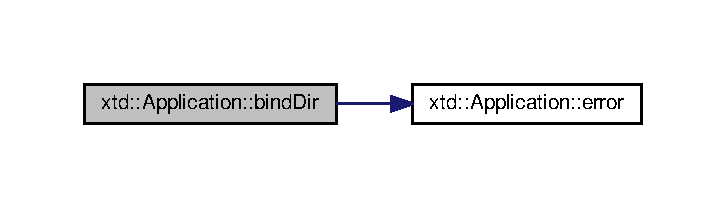
\includegraphics[width=347pt]{classxtd_1_1Application_a2b491ba745bbd3b2d01d9e623c0aff60_cgraph}
\end{center}
\end{figure}




Here is the caller graph for this function\+:
\nopagebreak
\begin{figure}[H]
\begin{center}
\leavevmode
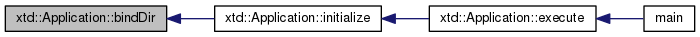
\includegraphics[width=350pt]{classxtd_1_1Application_a2b491ba745bbd3b2d01d9e623c0aff60_icgraph}
\end{center}
\end{figure}


\index{xtd\+::\+Application@{xtd\+::\+Application}!bind\+File@{bind\+File}}
\index{bind\+File@{bind\+File}!xtd\+::\+Application@{xtd\+::\+Application}}
\subsubsection[{\texorpdfstring{bind\+File(string \&p\+\_\+target, bool p\+\_\+readable=true) const }{bindFile(string &p_target, bool p_readable=true) const }}]{\setlength{\rightskip}{0pt plus 5cm}Application\+::t\+\_\+callback Application\+::bind\+File (
\begin{DoxyParamCaption}
\item[{string \&}]{p\+\_\+target, }
\item[{bool}]{p\+\_\+readable = {\ttfamily true}}
\end{DoxyParamCaption}
) const\hspace{0.3cm}{\ttfamily [protected]}}\hypertarget{classxtd_1_1Application_ab10f6dde0bf4034dff7eafe8a45c2029}{}\label{classxtd_1_1Application_ab10f6dde0bf4034dff7eafe8a45c2029}


Bind option\textquotesingle{}s parameter to a file name. 


\begin{DoxyParams}{Parameters}
{\em p\+\_\+target} & Reference variable to store the option\textquotesingle{}s value \\
\hline
{\em p\+\_\+readable} & If true, check that given file name exists and is readable \\
\hline
\end{DoxyParams}
\begin{DoxyReturn}{Returns}
generated option callback 
\end{DoxyReturn}


Definition at line 59 of file Application.\+cc.


\begin{DoxyCode}
60 \{
61   \textcolor{keywordflow}{return} [&p\_target, p\_readable, \textcolor{keyword}{this}](\textcolor{keyword}{const} \textcolor{keywordtype}{string}& p\_value, \textcolor{keyword}{const} t\_option& p\_opt) \{
62     p\_target = p\_value;
63     \textcolor{keywordflow}{if} (p\_readable && (\textcolor{keyword}{false} == boost::filesystem::exists(p\_value)))
64       \hyperlink{classxtd_1_1Application_adf84f52f1388bef1336d0fb5f6345563}{error}(1, \textcolor{stringliteral}{"invalid option -%c=%s, must be readable file"}, p\_opt.m\_shortOpt, p\_value);
65   \};
66 \}
\end{DoxyCode}


Here is the call graph for this function\+:
\nopagebreak
\begin{figure}[H]
\begin{center}
\leavevmode
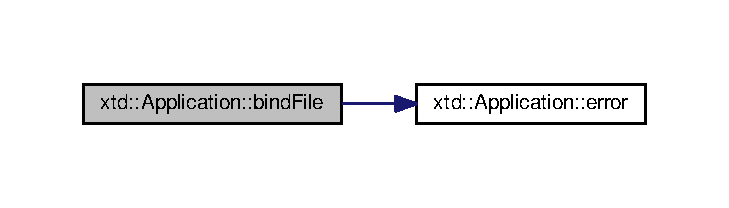
\includegraphics[width=350pt]{classxtd_1_1Application_ab10f6dde0bf4034dff7eafe8a45c2029_cgraph}
\end{center}
\end{figure}




Here is the caller graph for this function\+:
\nopagebreak
\begin{figure}[H]
\begin{center}
\leavevmode
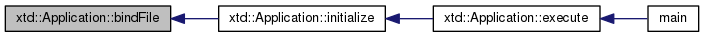
\includegraphics[width=350pt]{classxtd_1_1Application_ab10f6dde0bf4034dff7eafe8a45c2029_icgraph}
\end{center}
\end{figure}


\index{xtd\+::\+Application@{xtd\+::\+Application}!bind\+Given@{bind\+Given}}
\index{bind\+Given@{bind\+Given}!xtd\+::\+Application@{xtd\+::\+Application}}
\subsubsection[{\texorpdfstring{bind\+Given(bool \&p\+\_\+target) const }{bindGiven(bool &p_target) const }}]{\setlength{\rightskip}{0pt plus 5cm}Application\+::t\+\_\+callback Application\+::bind\+Given (
\begin{DoxyParamCaption}
\item[{bool \&}]{p\+\_\+target}
\end{DoxyParamCaption}
) const\hspace{0.3cm}{\ttfamily [protected]}}\hypertarget{classxtd_1_1Application_a59b986c85c2e1d9473f73df10425dfcf}{}\label{classxtd_1_1Application_a59b986c85c2e1d9473f73df10425dfcf}


Set targeted variable to true if option is given on command line. 


\begin{DoxyParams}{Parameters}
{\em p\+\_\+target} & Reference variable \\
\hline
\end{DoxyParams}
\begin{DoxyReturn}{Returns}
generated option callback 
\end{DoxyReturn}


Definition at line 93 of file Application.\+cc.


\begin{DoxyCode}
94 \{
95   p\_target = \textcolor{keyword}{false};
96   \textcolor{keywordflow}{return} [&p\_target](\textcolor{keyword}{const} \textcolor{keywordtype}{string}&, \textcolor{keyword}{const} t\_option&) \{
97     p\_target = \textcolor{keyword}{true};
98   \};
99 \}
\end{DoxyCode}


Here is the caller graph for this function\+:
\nopagebreak
\begin{figure}[H]
\begin{center}
\leavevmode
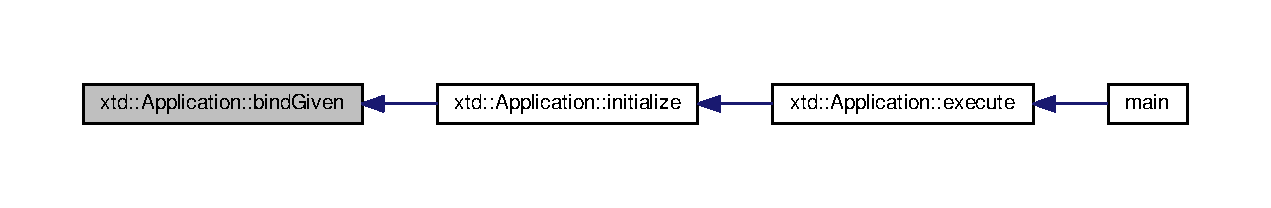
\includegraphics[width=350pt]{classxtd_1_1Application_a59b986c85c2e1d9473f73df10425dfcf_icgraph}
\end{center}
\end{figure}


\index{xtd\+::\+Application@{xtd\+::\+Application}!bind\+Number@{bind\+Number}}
\index{bind\+Number@{bind\+Number}!xtd\+::\+Application@{xtd\+::\+Application}}
\subsubsection[{\texorpdfstring{bind\+Number(\+T \&p\+\_\+target, T p\+\_\+min=std\+::numeric\+\_\+limits$<$ T $>$\+::min(), T p\+\_\+max=std\+::numeric\+\_\+limits$<$ T $>$\+::max()) const }{bindNumber(T &p_target, T p_min=std::numeric_limits< T >::min(), T p_max=std::numeric_limits< T >::max()) const }}]{\setlength{\rightskip}{0pt plus 5cm}template$<$typename T $>$ t\+\_\+callback xtd\+::\+Application\+::bind\+Number (
\begin{DoxyParamCaption}
\item[{T \&}]{p\+\_\+target, }
\item[{T}]{p\+\_\+min = {\ttfamily std\+:\+:numeric\+\_\+limits$<$~T~$>$\+:\+:min()}, }
\item[{T}]{p\+\_\+max = {\ttfamily std\+:\+:numeric\+\_\+limits$<$~T~$>$\+:\+:max()}}
\end{DoxyParamCaption}
) const\hspace{0.3cm}{\ttfamily [protected]}}\hypertarget{classxtd_1_1Application_ae5fd6c9b1d2ad5225f9d624f63df4173}{}\label{classxtd_1_1Application_ae5fd6c9b1d2ad5225f9d624f63df4173}


Bind option\textquotesingle{}s paramter as number to referenced variable. 


\begin{DoxyParams}{Parameters}
{\em p\+\_\+target} & Reference variable \\
\hline
{\em p\+\_\+min} & Minimum parameter value \mbox{[}inclusive\mbox{]} \\
\hline
{\em p\+\_\+max} & Maximum parameter value \mbox{[}inclusive\mbox{]} \\
\hline
\end{DoxyParams}
\begin{DoxyReturn}{Returns}
generated option callback
\end{DoxyReturn}
Will led to an error if input parameter \+:
\begin{DoxyItemize}
\item not lexically convertible to T
\item is lower than p\+\_\+min
\item is greater than p\+\_\+max 
\end{DoxyItemize}

Here is the caller graph for this function\+:
\nopagebreak
\begin{figure}[H]
\begin{center}
\leavevmode
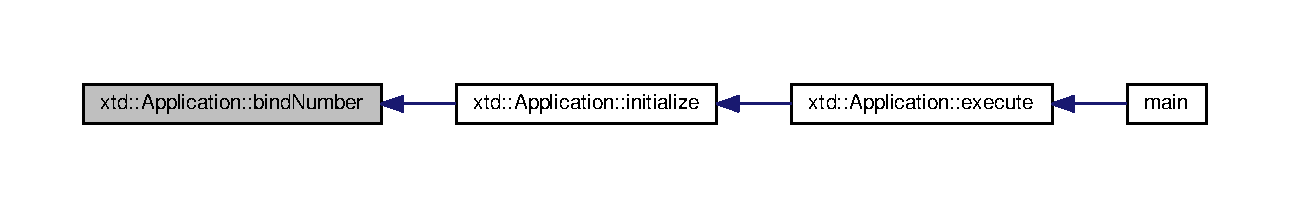
\includegraphics[width=350pt]{classxtd_1_1Application_ae5fd6c9b1d2ad5225f9d624f63df4173_icgraph}
\end{center}
\end{figure}


\index{xtd\+::\+Application@{xtd\+::\+Application}!bind\+String@{bind\+String}}
\index{bind\+String@{bind\+String}!xtd\+::\+Application@{xtd\+::\+Application}}
\subsubsection[{\texorpdfstring{bind\+String(string \&p\+\_\+target) const }{bindString(string &p_target) const }}]{\setlength{\rightskip}{0pt plus 5cm}Application\+::t\+\_\+callback Application\+::bind\+String (
\begin{DoxyParamCaption}
\item[{string \&}]{p\+\_\+target}
\end{DoxyParamCaption}
) const\hspace{0.3cm}{\ttfamily [protected]}}\hypertarget{classxtd_1_1Application_a36a351db3830e2e894a39fbd42842280}{}\label{classxtd_1_1Application_a36a351db3830e2e894a39fbd42842280}


Set targeted variable to option\textquotesingle{}s parameter. 


\begin{DoxyParams}{Parameters}
{\em p\+\_\+target} & Reference variable \\
\hline
\end{DoxyParams}
\begin{DoxyReturn}{Returns}
generated option callback 
\end{DoxyReturn}


Definition at line 83 of file Application.\+cc.


\begin{DoxyCode}
84 \{
85   \textcolor{keywordflow}{return} [&p\_target](\textcolor{keyword}{const} \textcolor{keywordtype}{string}& p\_value, \textcolor{keyword}{const} t\_option&) \{
86     p\_target = p\_value;
87   \};
88 
89 \}
\end{DoxyCode}


Here is the caller graph for this function\+:
\nopagebreak
\begin{figure}[H]
\begin{center}
\leavevmode
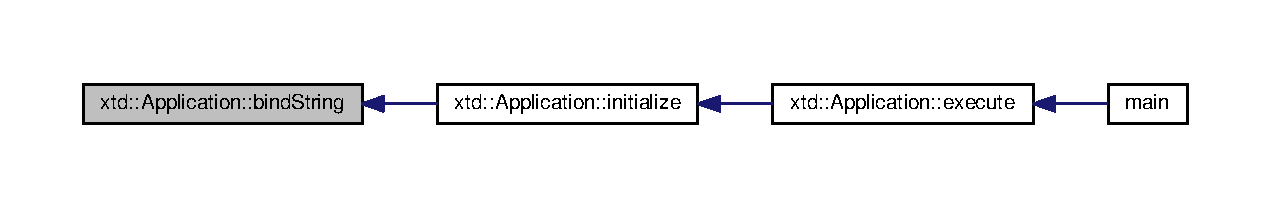
\includegraphics[width=350pt]{classxtd_1_1Application_a36a351db3830e2e894a39fbd42842280_icgraph}
\end{center}
\end{figure}


\index{xtd\+::\+Application@{xtd\+::\+Application}!bind\+Value\+If\+Given@{bind\+Value\+If\+Given}}
\index{bind\+Value\+If\+Given@{bind\+Value\+If\+Given}!xtd\+::\+Application@{xtd\+::\+Application}}
\subsubsection[{\texorpdfstring{bind\+Value\+If\+Given(\+T \&p\+\_\+target, const T \&p\+\_\+value) const }{bindValueIfGiven(T &p_target, const T &p_value) const }}]{\setlength{\rightskip}{0pt plus 5cm}template$<$typename T $>$ t\+\_\+callback xtd\+::\+Application\+::bind\+Value\+If\+Given (
\begin{DoxyParamCaption}
\item[{T \&}]{p\+\_\+target, }
\item[{const T \&}]{p\+\_\+value}
\end{DoxyParamCaption}
) const\hspace{0.3cm}{\ttfamily [protected]}}\hypertarget{classxtd_1_1Application_a2415acb66badb368e726173fb884097c}{}\label{classxtd_1_1Application_a2415acb66badb368e726173fb884097c}


Set given value to referenced variable if option is given. 


\begin{DoxyParams}{Parameters}
{\em p\+\_\+target} & Reference variable \\
\hline
{\em p\+\_\+value} & Value to set to p\+\_\+target \\
\hline
\end{DoxyParams}
\begin{DoxyReturn}{Returns}
generated option callback 
\end{DoxyReturn}


Here is the caller graph for this function\+:
\nopagebreak
\begin{figure}[H]
\begin{center}
\leavevmode
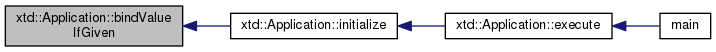
\includegraphics[width=350pt]{classxtd_1_1Application_a2415acb66badb368e726173fb884097c_icgraph}
\end{center}
\end{figure}


\index{xtd\+::\+Application@{xtd\+::\+Application}!bind\+Values@{bind\+Values}}
\index{bind\+Values@{bind\+Values}!xtd\+::\+Application@{xtd\+::\+Application}}
\subsubsection[{\texorpdfstring{bind\+Values(\+T \&p\+\_\+target, const Iterable \&p\+\_\+values) const }{bindValues(T &p_target, const Iterable &p_values) const }}]{\setlength{\rightskip}{0pt plus 5cm}template$<$typename T , class Iterable $>$ t\+\_\+callback xtd\+::\+Application\+::bind\+Values (
\begin{DoxyParamCaption}
\item[{T \&}]{p\+\_\+target, }
\item[{const Iterable \&}]{p\+\_\+values}
\end{DoxyParamCaption}
) const\hspace{0.3cm}{\ttfamily [protected]}}\hypertarget{classxtd_1_1Application_aaa0388f1c96893a26cfe5522b0804dd9}{}\label{classxtd_1_1Application_aaa0388f1c96893a26cfe5522b0804dd9}


Bind option\textquotesingle{}s parameter to target variable and checks among authorized values. 


\begin{DoxyParams}{Parameters}
{\em p\+\_\+target} & Reference variable \\
\hline
{\em p\+\_\+values} & Iterable container of authorized option\textquotesingle{}s values \\
\hline
\end{DoxyParams}
\begin{DoxyReturn}{Returns}
generated option callback 
\end{DoxyReturn}


Here is the caller graph for this function\+:
\nopagebreak
\begin{figure}[H]
\begin{center}
\leavevmode
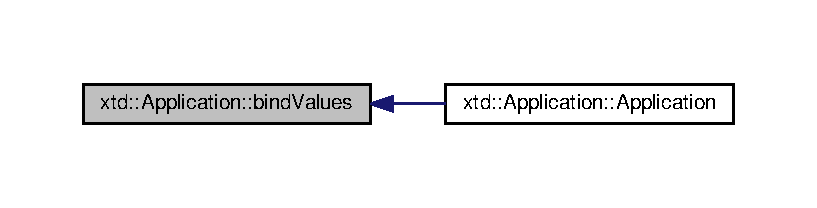
\includegraphics[width=350pt]{classxtd_1_1Application_aaa0388f1c96893a26cfe5522b0804dd9_icgraph}
\end{center}
\end{figure}


\index{xtd\+::\+Application@{xtd\+::\+Application}!check\+Options@{check\+Options}}
\index{check\+Options@{check\+Options}!xtd\+::\+Application@{xtd\+::\+Application}}
\subsubsection[{\texorpdfstring{check\+Options(void)}{checkOptions(void)}}]{\setlength{\rightskip}{0pt plus 5cm}virtual void xtd\+::\+Application\+::check\+Options (
\begin{DoxyParamCaption}
\item[{void}]{}
\end{DoxyParamCaption}
)\hspace{0.3cm}{\ttfamily [inline]}, {\ttfamily [protected]}, {\ttfamily [virtual]}}\hypertarget{classxtd_1_1Application_a3c63f070ac7baaea43a32b3064d0030b}{}\label{classxtd_1_1Application_a3c63f070ac7baaea43a32b3064d0030b}


Check read options, (default nothing) 



Definition at line 162 of file Application.\+hh.


\begin{DoxyCode}
162 \{\};
\end{DoxyCode}


Here is the caller graph for this function\+:
\nopagebreak
\begin{figure}[H]
\begin{center}
\leavevmode
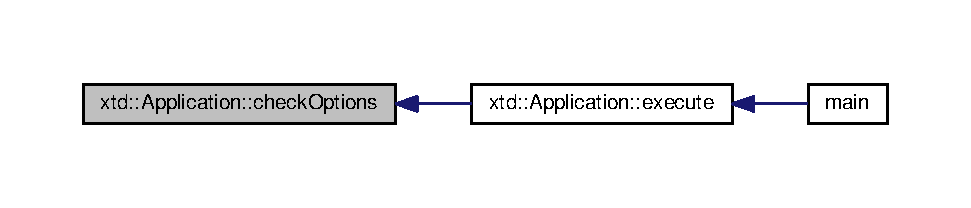
\includegraphics[width=350pt]{classxtd_1_1Application_a3c63f070ac7baaea43a32b3064d0030b_icgraph}
\end{center}
\end{figure}


\index{xtd\+::\+Application@{xtd\+::\+Application}!error@{error}}
\index{error@{error}!xtd\+::\+Application@{xtd\+::\+Application}}
\subsubsection[{\texorpdfstring{error(int p\+\_\+code, const string \&p\+\_\+format, Arguments \&\&...\+p\+\_\+args) const }{error(int p_code, const string &p_format, Arguments &&...p_args) const }}]{\setlength{\rightskip}{0pt plus 5cm}template$<$typename... Arguments$>$ void xtd\+::\+Application\+::error (
\begin{DoxyParamCaption}
\item[{int}]{p\+\_\+code, }
\item[{const string \&}]{p\+\_\+format, }
\item[{Arguments \&\&...}]{p\+\_\+args}
\end{DoxyParamCaption}
) const\hspace{0.3cm}{\ttfamily [protected]}}\hypertarget{classxtd_1_1Application_adf84f52f1388bef1336d0fb5f6345563}{}\label{classxtd_1_1Application_adf84f52f1388bef1336d0fb5f6345563}


Prints error and usage on standard error and exit. 


\begin{DoxyParams}{Parameters}
{\em p\+\_\+code} & exit code \\
\hline
{\em p\+\_\+format} & error message format (boost\+::format compatible) \\
\hline
{\em p\+\_\+args} & Template variadic arguments to format \\
\hline
\end{DoxyParams}


Here is the caller graph for this function\+:
\nopagebreak
\begin{figure}[H]
\begin{center}
\leavevmode
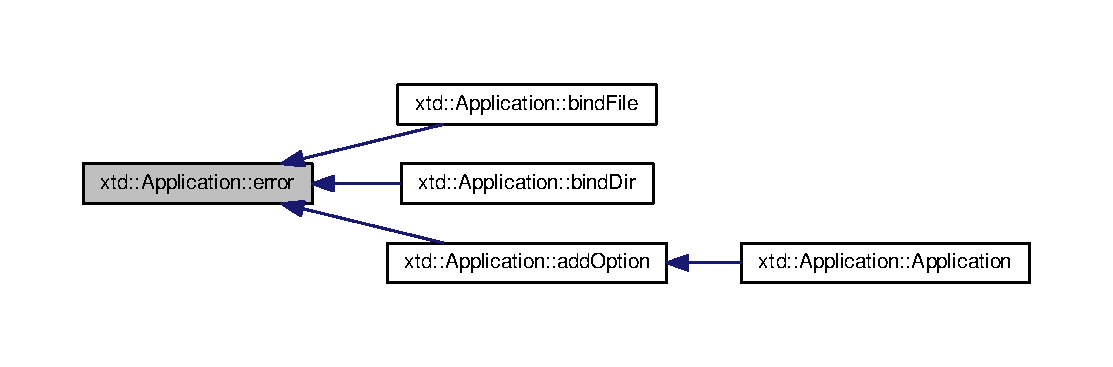
\includegraphics[width=350pt]{classxtd_1_1Application_adf84f52f1388bef1336d0fb5f6345563_icgraph}
\end{center}
\end{figure}


\index{xtd\+::\+Application@{xtd\+::\+Application}!error\+\_\+nohelp@{error\+\_\+nohelp}}
\index{error\+\_\+nohelp@{error\+\_\+nohelp}!xtd\+::\+Application@{xtd\+::\+Application}}
\subsubsection[{\texorpdfstring{error\+\_\+nohelp(int p\+\_\+code, const string \&p\+\_\+format, Arguments \&\&...\+p\+\_\+args) const }{error_nohelp(int p_code, const string &p_format, Arguments &&...p_args) const }}]{\setlength{\rightskip}{0pt plus 5cm}template$<$typename... Arguments$>$ void xtd\+::\+Application\+::error\+\_\+nohelp (
\begin{DoxyParamCaption}
\item[{int}]{p\+\_\+code, }
\item[{const string \&}]{p\+\_\+format, }
\item[{Arguments \&\&...}]{p\+\_\+args}
\end{DoxyParamCaption}
) const\hspace{0.3cm}{\ttfamily [protected]}}\hypertarget{classxtd_1_1Application_a810c6c1924f762fd453555cb91cb35f9}{}\label{classxtd_1_1Application_a810c6c1924f762fd453555cb91cb35f9}


Prints error on standard error and exit. 


\begin{DoxyParams}{Parameters}
{\em p\+\_\+code} & exit code \\
\hline
{\em p\+\_\+format} & error message format (boost\+::format compatible) \\
\hline
{\em p\+\_\+args} & Template variadic arguments to format \\
\hline
\end{DoxyParams}


Here is the caller graph for this function\+:
\nopagebreak
\begin{figure}[H]
\begin{center}
\leavevmode
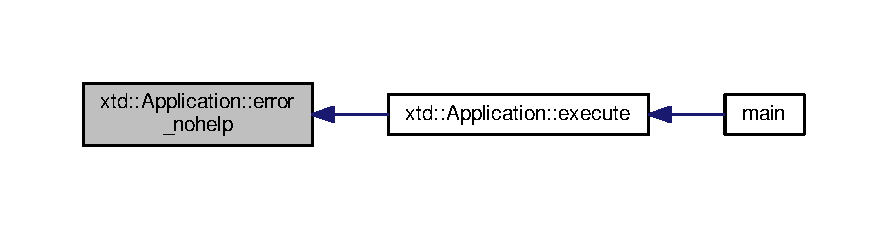
\includegraphics[width=350pt]{classxtd_1_1Application_a810c6c1924f762fd453555cb91cb35f9_icgraph}
\end{center}
\end{figure}


\index{xtd\+::\+Application@{xtd\+::\+Application}!execute@{execute}}
\index{execute@{execute}!xtd\+::\+Application@{xtd\+::\+Application}}
\subsubsection[{\texorpdfstring{execute(int p\+\_\+argc, char $\ast$$\ast$p\+\_\+argv)}{execute(int p_argc, char **p_argv)}}]{\setlength{\rightskip}{0pt plus 5cm}int Application\+::execute (
\begin{DoxyParamCaption}
\item[{int}]{p\+\_\+argc, }
\item[{char $\ast$$\ast$}]{p\+\_\+argv}
\end{DoxyParamCaption}
)}\hypertarget{classxtd_1_1Application_ae9241351a9caefa4b96bc906d3db144c}{}\label{classxtd_1_1Application_ae9241351a9caefa4b96bc906d3db144c}


main entry point, usually called with \hyperlink{doc_2example_2Application_8hh_a6b77b2233054447db17959182b5fb02b}{main(int,char$\ast$$\ast$)}\textquotesingle{}s arguments 


\begin{DoxyParams}{Parameters}
{\em p\+\_\+argc} & argument count \\
\hline
{\em p\+\_\+argv} & argument list (first is binary name) \\
\hline
\end{DoxyParams}
\begin{DoxyReturn}{Returns}
depends on \hyperlink{classxtd_1_1Application_aef6043d47982bc1983a84e2c8a53f0cd}{Application\+::process} implementation, usually 0 if process succeed 
\end{DoxyReturn}


Definition at line 103 of file Application.\+cc.


\begin{DoxyCode}
104 \{
105   \textcolor{keywordtype}{int} l\_status = 0;
106 
107   \textcolor{keywordflow}{try}
108   \{
109     \hyperlink{classxtd_1_1Application_abdf4c6f863c5a7a4ee842906f546c458}{m\_binName} = basename(p\_argv[0]);
110 
111     \hyperlink{classxtd_1_1logger_a21511dfdad9ec1e88c3444637a000e9d}{logger::get}().\hyperlink{classxtd_1_1logger_a586ddfe34d0f2c1343385f8034ef9b66}{initialize}(\textcolor{keywordtype}{string}(\hyperlink{classxtd_1_1Application_abdf4c6f863c5a7a4ee842906f546c458}{m\_binName}), 
      \hyperlink{classxtd_1_1logger_a250ce2f143da181d7149a1556da2a6f1a5888c6a8bb862595985926d16c7dcf13}{logger::level::crit});
112     readArgs(p\_argc, p\_argv);
113     \hyperlink{classxtd_1_1Application_a8684d1d061027893f91580106a821d88}{parseConfig}();
114     \hyperlink{classxtd_1_1Application_a3c63f070ac7baaea43a32b3064d0030b}{checkOptions}();
115     \hyperlink{classxtd_1_1logger_a21511dfdad9ec1e88c3444637a000e9d}{logger::get}().\hyperlink{classxtd_1_1logger_aeffebbe5b6a43f814c0a1251b6069f26}{setAllLevels}(\hyperlink{classxtd_1_1logger_a21511dfdad9ec1e88c3444637a000e9d}{logger::get}().levelOf(
      \hyperlink{classxtd_1_1Application_a3f815061d81aa12974b2b6ee48b9f5e9}{m\_logLevel}));
116     \hyperlink{classxtd_1_1Application_ab8e835ba678494c42e12c4613958d18a}{initialize}();
117 
118     m\_runThread = boost::thread(boost::bind(&boost::asio::io\_service::run, &m\_ioService));
119 
120     l\_status = \hyperlink{classxtd_1_1Application_aef6043d47982bc1983a84e2c8a53f0cd}{process}();
121 
122     m\_ioService.stop();
123     m\_runThread.join();
124   \}
125   \textcolor{keywordflow}{catch} (std::exception& l\_error) \{
126     \hyperlink{classxtd_1_1Application_a810c6c1924f762fd453555cb91cb35f9}{error\_nohelp}(1, \textcolor{stringliteral}{"caught exception : %s"}, l\_error.what());
127   \}
128 
129   \textcolor{keywordflow}{return} l\_status;
130 \}
\end{DoxyCode}


Here is the call graph for this function\+:
\nopagebreak
\begin{figure}[H]
\begin{center}
\leavevmode
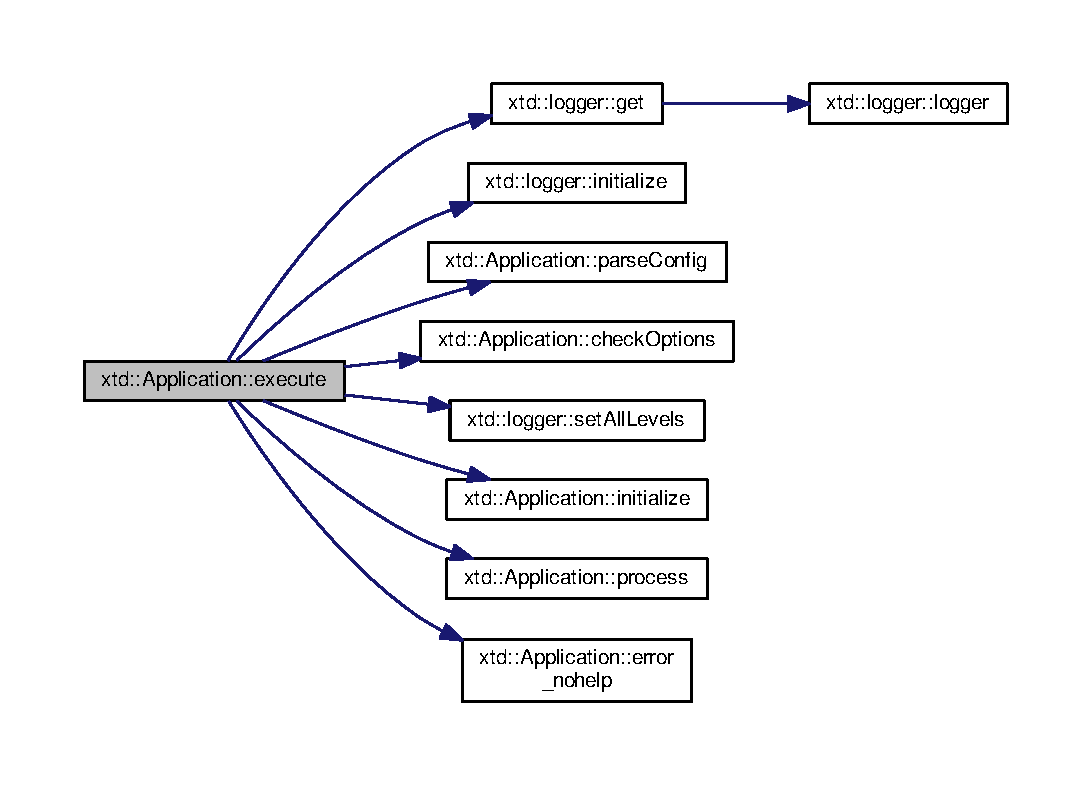
\includegraphics[width=350pt]{classxtd_1_1Application_ae9241351a9caefa4b96bc906d3db144c_cgraph}
\end{center}
\end{figure}




Here is the caller graph for this function\+:
\nopagebreak
\begin{figure}[H]
\begin{center}
\leavevmode
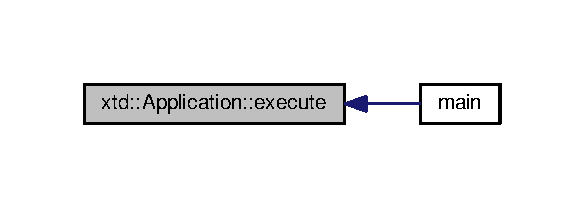
\includegraphics[width=279pt]{classxtd_1_1Application_ae9241351a9caefa4b96bc906d3db144c_icgraph}
\end{center}
\end{figure}


\index{xtd\+::\+Application@{xtd\+::\+Application}!get\+Version@{get\+Version}}
\index{get\+Version@{get\+Version}!xtd\+::\+Application@{xtd\+::\+Application}}
\subsubsection[{\texorpdfstring{get\+Version(void) const }{getVersion(void) const }}]{\setlength{\rightskip}{0pt plus 5cm}const string \& Application\+::get\+Version (
\begin{DoxyParamCaption}
\item[{void}]{}
\end{DoxyParamCaption}
) const\hspace{0.3cm}{\ttfamily [protected]}}\hypertarget{classxtd_1_1Application_ab7be8fa583daa66271562a83817b172c}{}\label{classxtd_1_1Application_ab7be8fa583daa66271562a83817b172c}


Get R\+C\+S\+ID identity informations. 



Definition at line 52 of file Application.\+cc.


\begin{DoxyCode}
53 \{
54   \textcolor{keywordflow}{return} \hyperlink{classxtd_1_1Application_ad820953bc15b729ce010f422595d3a3f}{m\_rcsid};
55 \}
\end{DoxyCode}


Here is the caller graph for this function\+:
\nopagebreak
\begin{figure}[H]
\begin{center}
\leavevmode
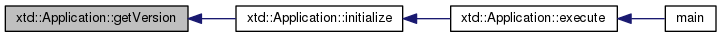
\includegraphics[width=350pt]{classxtd_1_1Application_ab7be8fa583daa66271562a83817b172c_icgraph}
\end{center}
\end{figure}


\index{xtd\+::\+Application@{xtd\+::\+Application}!initialize@{initialize}}
\index{initialize@{initialize}!xtd\+::\+Application@{xtd\+::\+Application}}
\subsubsection[{\texorpdfstring{initialize(void)}{initialize(void)}}]{\setlength{\rightskip}{0pt plus 5cm}virtual void xtd\+::\+Application\+::initialize (
\begin{DoxyParamCaption}
\item[{void}]{}
\end{DoxyParamCaption}
)\hspace{0.3cm}{\ttfamily [inline]}, {\ttfamily [protected]}, {\ttfamily [virtual]}}\hypertarget{classxtd_1_1Application_ab8e835ba678494c42e12c4613958d18a}{}\label{classxtd_1_1Application_ab8e835ba678494c42e12c4613958d18a}


initialize application, (default nothing) 



Definition at line 167 of file Application.\+hh.


\begin{DoxyCode}
167 \{\};
\end{DoxyCode}


Here is the call graph for this function\+:
\nopagebreak
\begin{figure}[H]
\begin{center}
\leavevmode
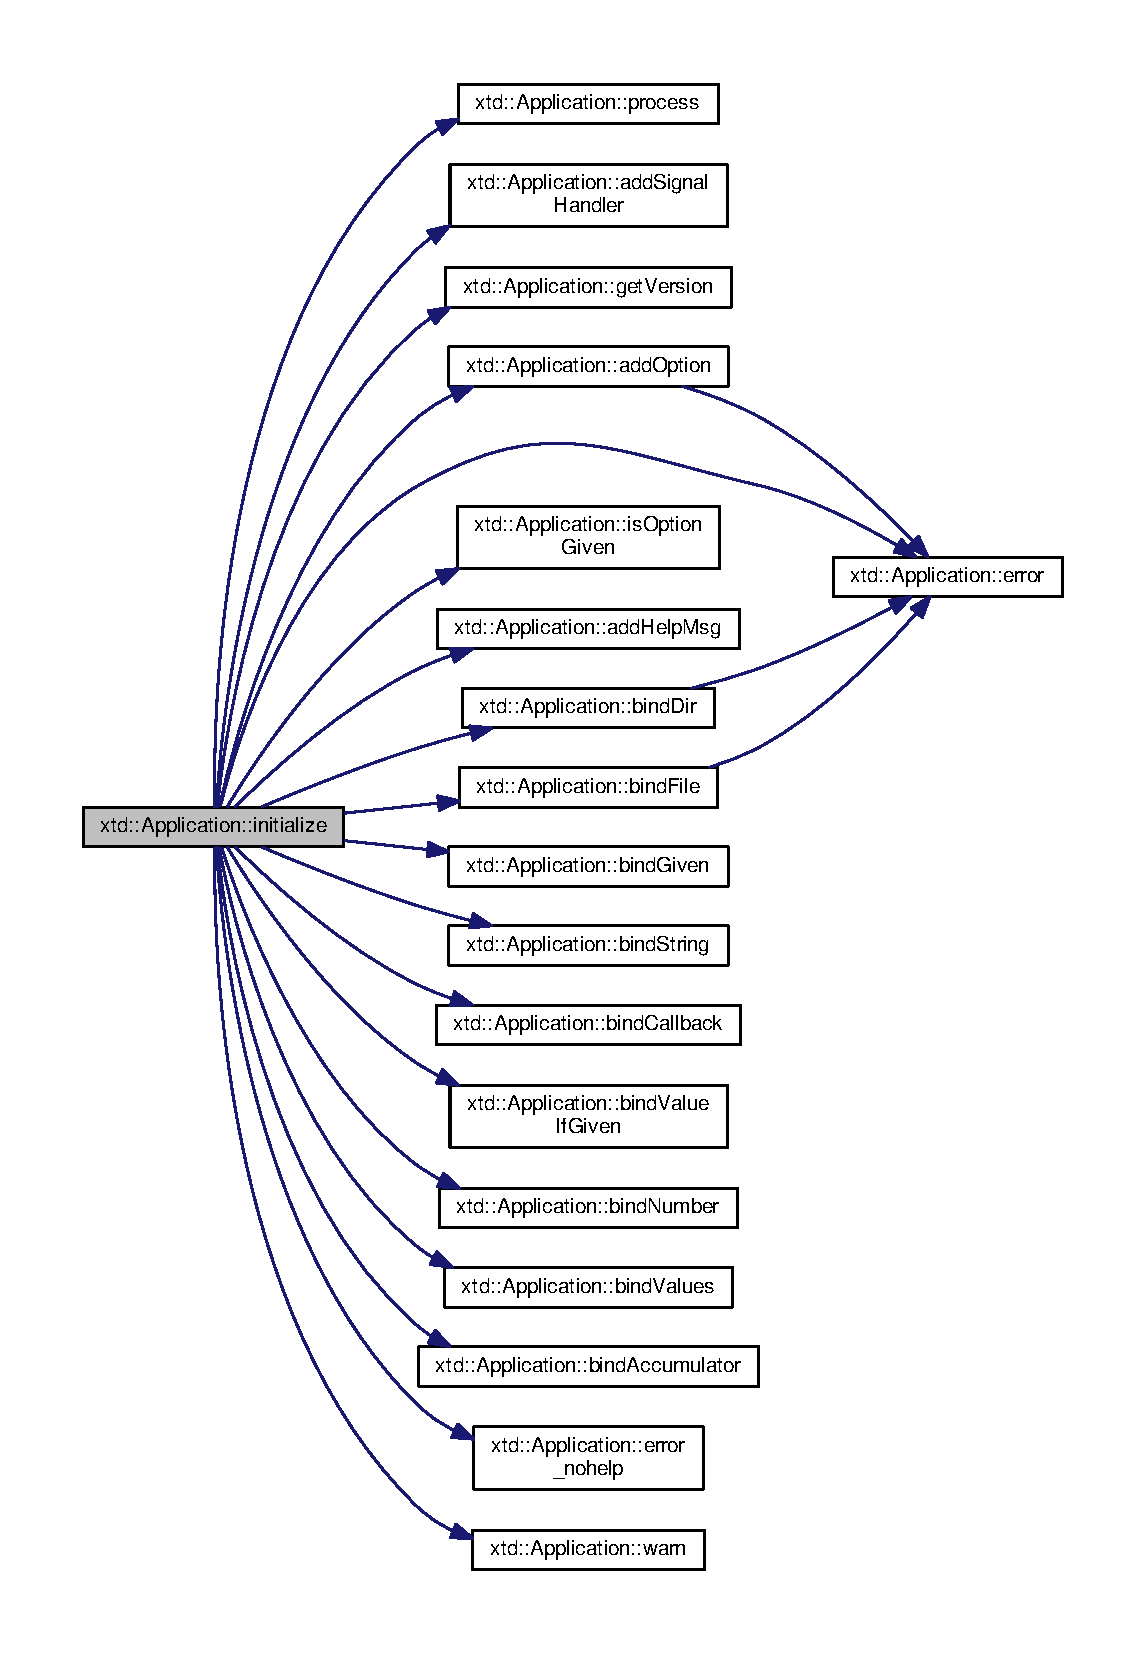
\includegraphics[width=350pt]{classxtd_1_1Application_ab8e835ba678494c42e12c4613958d18a_cgraph}
\end{center}
\end{figure}




Here is the caller graph for this function\+:
\nopagebreak
\begin{figure}[H]
\begin{center}
\leavevmode
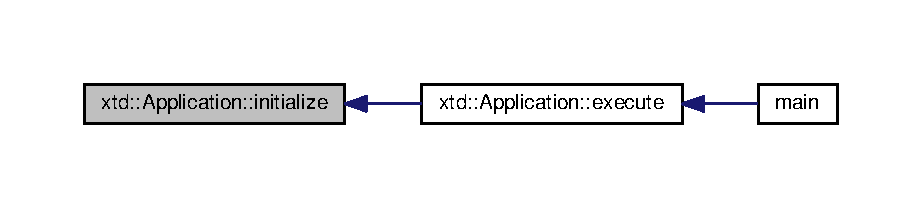
\includegraphics[width=350pt]{classxtd_1_1Application_ab8e835ba678494c42e12c4613958d18a_icgraph}
\end{center}
\end{figure}


\index{xtd\+::\+Application@{xtd\+::\+Application}!is\+Option\+Given@{is\+Option\+Given}}
\index{is\+Option\+Given@{is\+Option\+Given}!xtd\+::\+Application@{xtd\+::\+Application}}
\subsubsection[{\texorpdfstring{is\+Option\+Given(const string \&p\+\_\+option\+Name) const }{isOptionGiven(const string &p_optionName) const }}]{\setlength{\rightskip}{0pt plus 5cm}bool Application\+::is\+Option\+Given (
\begin{DoxyParamCaption}
\item[{const string \&}]{p\+\_\+option\+Name}
\end{DoxyParamCaption}
) const\hspace{0.3cm}{\ttfamily [protected]}}\hypertarget{classxtd_1_1Application_a4aca412c4a0bcd761e28b0350bd71578}{}\label{classxtd_1_1Application_a4aca412c4a0bcd761e28b0350bd71578}


Tells if given option was given on command line. 


\begin{DoxyParams}{Parameters}
{\em p\+\_\+option\+Name} & long-\/form or short-\/form of the option \\
\hline
\end{DoxyParams}
\begin{DoxyReturn}{Returns}
true if option was given 
\end{DoxyReturn}


Definition at line 286 of file Application.\+cc.


\begin{DoxyCode}
287 \{
288   \textcolor{keywordflow}{for} (\textcolor{keyword}{auto} cc\_opt = m\_optionList.begin();
289        cc\_opt != m\_optionList.end();
290        cc\_opt++)
291   \{
292     \textcolor{keywordtype}{string} l\_shortOpt;
293 
294     l\_shortOpt += cc\_opt->m\_shortOpt;
295 
296     \textcolor{keywordflow}{if} ((cc\_opt->m\_given    == \textcolor{keyword}{true}) &&
297         ((l\_shortOpt        == p\_optionName) ||
298          (cc\_opt->m\_longOpt == p\_optionName)))
299     \{
300       \textcolor{keywordflow}{return} \textcolor{keyword}{true};
301     \}
302   \}
303   \textcolor{keywordflow}{return} \textcolor{keyword}{false};
304 \}
\end{DoxyCode}


Here is the caller graph for this function\+:
\nopagebreak
\begin{figure}[H]
\begin{center}
\leavevmode
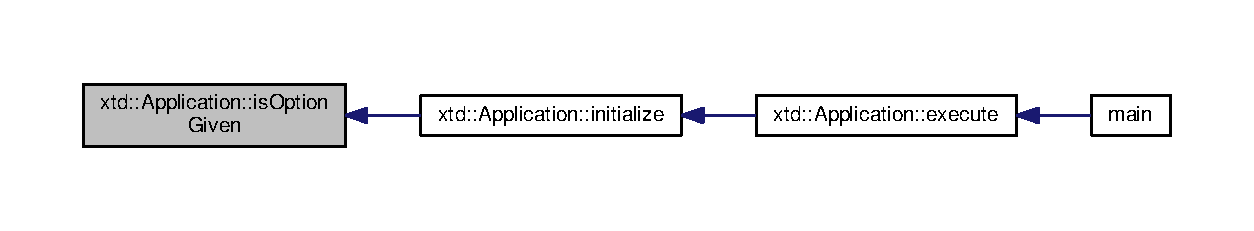
\includegraphics[width=350pt]{classxtd_1_1Application_a4aca412c4a0bcd761e28b0350bd71578_icgraph}
\end{center}
\end{figure}


\index{xtd\+::\+Application@{xtd\+::\+Application}!parse\+Config@{parse\+Config}}
\index{parse\+Config@{parse\+Config}!xtd\+::\+Application@{xtd\+::\+Application}}
\subsubsection[{\texorpdfstring{parse\+Config(void)}{parseConfig(void)}}]{\setlength{\rightskip}{0pt plus 5cm}virtual void xtd\+::\+Application\+::parse\+Config (
\begin{DoxyParamCaption}
\item[{void}]{}
\end{DoxyParamCaption}
)\hspace{0.3cm}{\ttfamily [inline]}, {\ttfamily [protected]}, {\ttfamily [virtual]}}\hypertarget{classxtd_1_1Application_a8684d1d061027893f91580106a821d88}{}\label{classxtd_1_1Application_a8684d1d061027893f91580106a821d88}


Parse application configuration, (default nothing) 



Definition at line 157 of file Application.\+hh.


\begin{DoxyCode}
157 \{\};
\end{DoxyCode}


Here is the caller graph for this function\+:
\nopagebreak
\begin{figure}[H]
\begin{center}
\leavevmode
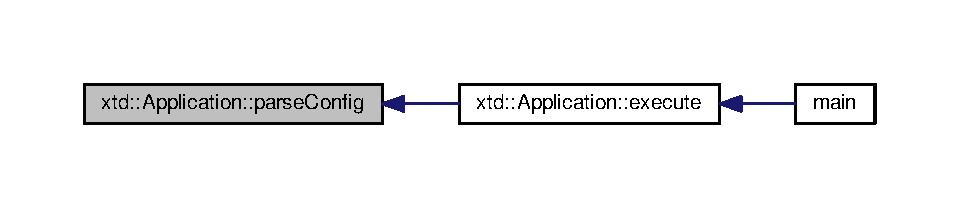
\includegraphics[width=350pt]{classxtd_1_1Application_a8684d1d061027893f91580106a821d88_icgraph}
\end{center}
\end{figure}


\index{xtd\+::\+Application@{xtd\+::\+Application}!process@{process}}
\index{process@{process}!xtd\+::\+Application@{xtd\+::\+Application}}
\subsubsection[{\texorpdfstring{process(void)}{process(void)}}]{\setlength{\rightskip}{0pt plus 5cm}int Application\+::process (
\begin{DoxyParamCaption}
\item[{void}]{}
\end{DoxyParamCaption}
)\hspace{0.3cm}{\ttfamily [protected]}, {\ttfamily [virtual]}}\hypertarget{classxtd_1_1Application_aef6043d47982bc1983a84e2c8a53f0cd}{}\label{classxtd_1_1Application_aef6043d47982bc1983a84e2c8a53f0cd}


Main application process function, (default nothing) 

\begin{DoxyReturn}{Returns}
Up to the user, generally 0 in case of success 
\end{DoxyReturn}


Definition at line 166 of file Application.\+cc.


\begin{DoxyCode}
167 \{
168   \textcolor{keywordflow}{return} 0;
169 \}
\end{DoxyCode}


Here is the caller graph for this function\+:
\nopagebreak
\begin{figure}[H]
\begin{center}
\leavevmode
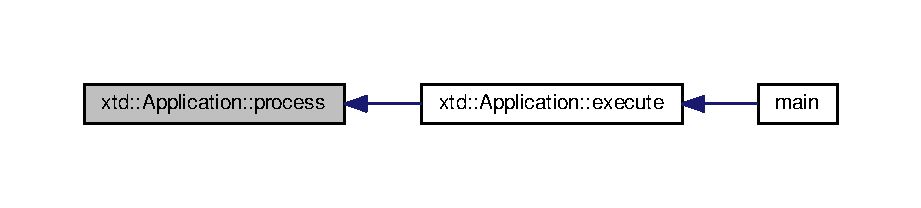
\includegraphics[width=350pt]{classxtd_1_1Application_aef6043d47982bc1983a84e2c8a53f0cd_icgraph}
\end{center}
\end{figure}


\index{xtd\+::\+Application@{xtd\+::\+Application}!warn@{warn}}
\index{warn@{warn}!xtd\+::\+Application@{xtd\+::\+Application}}
\subsubsection[{\texorpdfstring{warn(const string \&p\+\_\+format, Arguments \&\&...\+p\+\_\+args) const }{warn(const string &p_format, Arguments &&...p_args) const }}]{\setlength{\rightskip}{0pt plus 5cm}template$<$typename... Arguments$>$ void xtd\+::\+Application\+::warn (
\begin{DoxyParamCaption}
\item[{const string \&}]{p\+\_\+format, }
\item[{Arguments \&\&...}]{p\+\_\+args}
\end{DoxyParamCaption}
) const\hspace{0.3cm}{\ttfamily [protected]}}\hypertarget{classxtd_1_1Application_a931877468f6b948909d596d91d60b7a2}{}\label{classxtd_1_1Application_a931877468f6b948909d596d91d60b7a2}


Prints a warning on standard error. 


\begin{DoxyParams}{Parameters}
{\em p\+\_\+format} & error message format (boost\+::format compatible) \\
\hline
{\em p\+\_\+args} & Template variadic arguments to format \\
\hline
\end{DoxyParams}


Here is the caller graph for this function\+:
\nopagebreak
\begin{figure}[H]
\begin{center}
\leavevmode
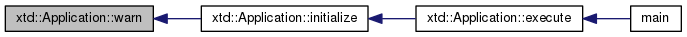
\includegraphics[width=350pt]{classxtd_1_1Application_a931877468f6b948909d596d91d60b7a2_icgraph}
\end{center}
\end{figure}




\subsection{Member Data Documentation}
\index{xtd\+::\+Application@{xtd\+::\+Application}!m\+\_\+bin\+Name@{m\+\_\+bin\+Name}}
\index{m\+\_\+bin\+Name@{m\+\_\+bin\+Name}!xtd\+::\+Application@{xtd\+::\+Application}}
\subsubsection[{\texorpdfstring{m\+\_\+bin\+Name}{m_binName}}]{\setlength{\rightskip}{0pt plus 5cm}string xtd\+::\+Application\+::m\+\_\+bin\+Name\hspace{0.3cm}{\ttfamily [protected]}}\hypertarget{classxtd_1_1Application_abdf4c6f863c5a7a4ee842906f546c458}{}\label{classxtd_1_1Application_abdf4c6f863c5a7a4ee842906f546c458}


binary name (argv\mbox{[}0\mbox{]}) 



Definition at line 339 of file Application.\+hh.

\index{xtd\+::\+Application@{xtd\+::\+Application}!m\+\_\+log\+Level@{m\+\_\+log\+Level}}
\index{m\+\_\+log\+Level@{m\+\_\+log\+Level}!xtd\+::\+Application@{xtd\+::\+Application}}
\subsubsection[{\texorpdfstring{m\+\_\+log\+Level}{m_logLevel}}]{\setlength{\rightskip}{0pt plus 5cm}uint32\+\_\+t xtd\+::\+Application\+::m\+\_\+log\+Level\hspace{0.3cm}{\ttfamily [protected]}}\hypertarget{classxtd_1_1Application_a3f815061d81aa12974b2b6ee48b9f5e9}{}\label{classxtd_1_1Application_a3f815061d81aa12974b2b6ee48b9f5e9}


log level read from command line 



Definition at line 340 of file Application.\+hh.

\index{xtd\+::\+Application@{xtd\+::\+Application}!m\+\_\+rcsid@{m\+\_\+rcsid}}
\index{m\+\_\+rcsid@{m\+\_\+rcsid}!xtd\+::\+Application@{xtd\+::\+Application}}
\subsubsection[{\texorpdfstring{m\+\_\+rcsid}{m_rcsid}}]{\setlength{\rightskip}{0pt plus 5cm}string xtd\+::\+Application\+::m\+\_\+rcsid\hspace{0.3cm}{\ttfamily [protected]}}\hypertarget{classxtd_1_1Application_ad820953bc15b729ce010f422595d3a3f}{}\label{classxtd_1_1Application_ad820953bc15b729ce010f422595d3a3f}


binary identity information 



Definition at line 342 of file Application.\+hh.

\index{xtd\+::\+Application@{xtd\+::\+Application}!m\+\_\+remaining\+Args@{m\+\_\+remaining\+Args}}
\index{m\+\_\+remaining\+Args@{m\+\_\+remaining\+Args}!xtd\+::\+Application@{xtd\+::\+Application}}
\subsubsection[{\texorpdfstring{m\+\_\+remaining\+Args}{m_remainingArgs}}]{\setlength{\rightskip}{0pt plus 5cm}vector$<$string$>$ xtd\+::\+Application\+::m\+\_\+remaining\+Args\hspace{0.3cm}{\ttfamily [protected]}}\hypertarget{classxtd_1_1Application_a7651fd3849530cdded556187a6b42c25}{}\label{classxtd_1_1Application_a7651fd3849530cdded556187a6b42c25}


positional command line arguments 



Definition at line 341 of file Application.\+hh.



The documentation for this class was generated from the following files\+:\begin{DoxyCompactItemize}
\item 
/home/psyco/dev/xtdcpp/common/src/\hyperlink{src_2Application_8hh}{Application.\+hh}\item 
/home/psyco/dev/xtdcpp/common/src/\hyperlink{Application_8cc}{Application.\+cc}\end{DoxyCompactItemize}

\hypertarget{classxtd_1_1ConfParser}{\section{xtd\-:\-:Conf\-Parser Class Reference}
\label{classxtd_1_1ConfParser}\index{xtd\-::\-Conf\-Parser@{xtd\-::\-Conf\-Parser}}
}


{\ttfamily \#include $<$Conf\-Parser.\-hh$>$}



Collaboration diagram for xtd\-:\-:Conf\-Parser\-:
\nopagebreak
\begin{figure}[H]
\begin{center}
\leavevmode
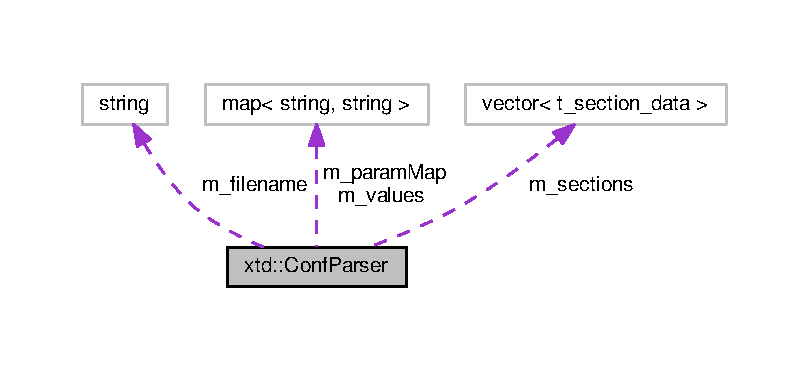
\includegraphics[width=350pt]{classxtd_1_1ConfParser__coll__graph}
\end{center}
\end{figure}
\subsection*{Classes}
\begin{DoxyCompactItemize}
\item 
class \hyperlink{classxtd_1_1ConfParser_1_1const__iterator}{const\-\_\-iterator}
\end{DoxyCompactItemize}
\subsection*{Public Types}
\begin{DoxyCompactItemize}
\item 
typedef map$<$ string, string $>$ \hyperlink{classxtd_1_1ConfParser_a715a3e39fd796046c94546e60f22414d}{t\-\_\-param\-\_\-map}
\item 
typedef boost\-::shared\-\_\-ptr\\*
$<$ \hyperlink{classxtd_1_1ConfParser}{Conf\-Parser} $>$ \hyperlink{classxtd_1_1ConfParser_ae1e724e304256650bac2e9b2d63a51df}{t\-\_\-sptr}
\end{DoxyCompactItemize}
\subsection*{Public Member Functions}
\begin{DoxyCompactItemize}
\item 
\hyperlink{classxtd_1_1ConfParser_a5f7729df32b946dba9690494b6fee762}{Conf\-Parser} (const string \&p\-\_\-path)
\item 
\hyperlink{classxtd_1_1ConfParser_a460c904cfe815a6141feb088022c9564}{Conf\-Parser} (const string \&p\-\_\-path, const \hyperlink{classxtd_1_1ConfParser_a715a3e39fd796046c94546e60f22414d}{t\-\_\-param\-\_\-map} \&p\-\_\-params)
\item 
const string \& \hyperlink{classxtd_1_1ConfParser_a2a72cefc513e103b86d90785862c620f}{get\-File\-Path} (void) const 
\item 
\hyperlink{classxtd_1_1ConfParser_1_1const__iterator}{const\-\_\-iterator} \hyperlink{classxtd_1_1ConfParser_a18acbfe7e5828eff045bdcc941626974}{find} (const char $\ast$p\-\_\-name) const 
\item 
\hyperlink{classxtd_1_1ConfParser_1_1const__iterator}{const\-\_\-iterator} \hyperlink{classxtd_1_1ConfParser_aff7ee8bcd3de4359eff719bc4a6570ba}{find} (const string \&p\-\_\-key) const 
\item 
\hyperlink{classxtd_1_1ConfParser_1_1const__iterator}{const\-\_\-iterator} \hyperlink{classxtd_1_1ConfParser_ab772ae8e571f1a3f719eca2f9d056d7c}{end} (void) const 
\item 
\hyperlink{classxtd_1_1ConfParser_1_1const__iterator}{const\-\_\-iterator} \hyperlink{classxtd_1_1ConfParser_a18fa4083def8aaf86796b9ddbc331daf}{begin} (void) const 
\item 
\hyperlink{namespacextd_a68ed4fe8e9c11116b68efe5b102aec50}{status} \hyperlink{classxtd_1_1ConfParser_a5ef18d8778c844ce60f2c93579be7926}{get} (const string \&p\-\_\-name, string \&p\-\_\-dval) const 
\item 
\hyperlink{namespacextd_a68ed4fe8e9c11116b68efe5b102aec50}{status} \hyperlink{classxtd_1_1ConfParser_ac8f46e56cdd5d015719c682707b12bc2}{get} (const string \&p\-\_\-name, const char $\ast$\&p\-\_\-dval) const 
\item 
\hyperlink{namespacextd_a68ed4fe8e9c11116b68efe5b102aec50}{status} \hyperlink{classxtd_1_1ConfParser_adaf860ed87b32df2ac16f73cab8bbbed}{get} (const string \&p\-\_\-name, char \&p\-\_\-ival) const 
\item 
\hyperlink{namespacextd_a68ed4fe8e9c11116b68efe5b102aec50}{status} \hyperlink{classxtd_1_1ConfParser_a6edfffe778ba93a7dc0ce3b71e1a293d}{get} (const string \&p\-\_\-name, unsigned char \&p\-\_\-ival) const 
\item 
\hyperlink{namespacextd_a68ed4fe8e9c11116b68efe5b102aec50}{status} \hyperlink{classxtd_1_1ConfParser_abd0bb9c9e8568c0b2dd28b133f700681}{get} (const string \&p\-\_\-name, unsigned short \&p\-\_\-ival) const 
\item 
\hyperlink{namespacextd_a68ed4fe8e9c11116b68efe5b102aec50}{status} \hyperlink{classxtd_1_1ConfParser_a902dfe3ab82e8d1710659f65fa0e853b}{get} (const string \&p\-\_\-name, int \&p\-\_\-ival) const 
\item 
\hyperlink{namespacextd_a68ed4fe8e9c11116b68efe5b102aec50}{status} \hyperlink{classxtd_1_1ConfParser_aeabbb63eeeafaf9d0853fdcf5b2a83eb}{get} (const string \&p\-\_\-name, long \&p\-\_\-ival) const 
\item 
\hyperlink{namespacextd_a68ed4fe8e9c11116b68efe5b102aec50}{status} \hyperlink{classxtd_1_1ConfParser_a38c007fd9a93cf370a9e2de14e021faf}{get} (const string \&p\-\_\-name, unsigned long long \&p\-\_\-ival) const 
\item 
\hyperlink{namespacextd_a68ed4fe8e9c11116b68efe5b102aec50}{status} \hyperlink{classxtd_1_1ConfParser_a39e678dc0205b82f4cce76533f4f4d84}{get} (const string \&p\-\_\-name, unsigned long \&p\-\_\-ival) const 
\item 
\hyperlink{namespacextd_a68ed4fe8e9c11116b68efe5b102aec50}{status} \hyperlink{classxtd_1_1ConfParser_a1e8fd9399881ef9910fd144377ff4c93}{get} (const string \&p\-\_\-name, unsigned int \&p\-\_\-ival) const 
\item 
\hyperlink{namespacextd_a68ed4fe8e9c11116b68efe5b102aec50}{status} \hyperlink{classxtd_1_1ConfParser_a6d091368a02f05c377c7d27d748b64be}{get} (const string \&p\-\_\-name, double \&p\-\_\-dval) const 
\item 
\hyperlink{namespacextd_a68ed4fe8e9c11116b68efe5b102aec50}{status} \hyperlink{classxtd_1_1ConfParser_ac0d9efc31b6b6989f4a9f6061ad03596}{get} (const string \&p\-\_\-name, float \&p\-\_\-dval) const 
\item 
\hyperlink{namespacextd_a68ed4fe8e9c11116b68efe5b102aec50}{status} \hyperlink{classxtd_1_1ConfParser_a8a8e729b8e11c5efd19dec29baa31f66}{get} (const string \&p\-\_\-name, bool \&p\-\_\-dval) const 
\item 
{\footnotesize template$<$typename T $>$ }\\\hyperlink{namespacextd_a68ed4fe8e9c11116b68efe5b102aec50}{status} \hyperlink{classxtd_1_1ConfParser_aa3a209f68c61547141194a305049eeae}{get\-\_\-default} (const string \&p\-\_\-key, T \&p\-\_\-dest, const T \&p\-\_\-default)
\item 
bool \hyperlink{classxtd_1_1ConfParser_a7f1323a9ef1f85c73a0bff383e24967c}{exists} (const string \&p\-\_\-name) const 
\begin{DoxyCompactList}\small\item\em Indique si la clef p\-\_\-name existe dans le fichier de conf. \end{DoxyCompactList}\item 
void \hyperlink{classxtd_1_1ConfParser_ae7e7ade9440517b79cc22f21b10df7a5}{dump\-Keys} (std\-::ostream \&p\-\_\-stream) const 
\item 
const \hyperlink{classxtd_1_1ConfParser_a715a3e39fd796046c94546e60f22414d}{t\-\_\-param\-\_\-map} \& \hyperlink{classxtd_1_1ConfParser_a1be1c2813abf959d85bb6cf695c74dec}{get\-Param\-Map} (void) const 
\item 
const t\-\_\-value\-\_\-map \& \hyperlink{classxtd_1_1ConfParser_a34d7366228341b5501bfec94607dd396}{get\-Value\-Map} (void) const 
\end{DoxyCompactItemize}
\subsection*{Protected Attributes}
\begin{DoxyCompactItemize}
\item 
t\-\_\-value\-\_\-map \hyperlink{classxtd_1_1ConfParser_a4c58cc4fa96ebaddd180a0c67edb481f}{m\-\_\-values}
\item 
t\-\_\-section\-\_\-list \hyperlink{classxtd_1_1ConfParser_a100cffb5f33795e50c87ab5fb2a43963}{m\-\_\-sections}
\item 
int \hyperlink{classxtd_1_1ConfParser_a5203f3b8cb6e9070b33371c9acabbc8c}{m\-\_\-nblines}
\item 
string \hyperlink{classxtd_1_1ConfParser_abc9e0b073f91de77b76db39bfbc27508}{m\-\_\-filename}
\item 
\hyperlink{classxtd_1_1ConfParser_a715a3e39fd796046c94546e60f22414d}{t\-\_\-param\-\_\-map} \hyperlink{classxtd_1_1ConfParser_abe309999c7964603bde870c7bda16d2e}{m\-\_\-param\-Map}
\end{DoxyCompactItemize}


\subsection{Detailed Description}
this class read a file whose format is describe in ??? information can then be recovered via use of \hyperlink{classxtd_1_1ConfParser_a5ef18d8778c844ce60f2c93579be7926}{get()} member function 

Definition at line 23 of file Conf\-Parser.\-hh.



\subsection{Member Typedef Documentation}
\hypertarget{classxtd_1_1ConfParser_a715a3e39fd796046c94546e60f22414d}{\index{xtd\-::\-Conf\-Parser@{xtd\-::\-Conf\-Parser}!t\-\_\-param\-\_\-map@{t\-\_\-param\-\_\-map}}
\index{t\-\_\-param\-\_\-map@{t\-\_\-param\-\_\-map}!xtd::ConfParser@{xtd\-::\-Conf\-Parser}}
\subsubsection[{t\-\_\-param\-\_\-map}]{\setlength{\rightskip}{0pt plus 5cm}typedef map$<$string, string$>$ {\bf xtd\-::\-Conf\-Parser\-::t\-\_\-param\-\_\-map}}}\label{classxtd_1_1ConfParser_a715a3e39fd796046c94546e60f22414d}


Definition at line 31 of file Conf\-Parser.\-hh.

\hypertarget{classxtd_1_1ConfParser_ae1e724e304256650bac2e9b2d63a51df}{\index{xtd\-::\-Conf\-Parser@{xtd\-::\-Conf\-Parser}!t\-\_\-sptr@{t\-\_\-sptr}}
\index{t\-\_\-sptr@{t\-\_\-sptr}!xtd::ConfParser@{xtd\-::\-Conf\-Parser}}
\subsubsection[{t\-\_\-sptr}]{\setlength{\rightskip}{0pt plus 5cm}typedef boost\-::shared\-\_\-ptr$<${\bf Conf\-Parser}$>$ {\bf xtd\-::\-Conf\-Parser\-::t\-\_\-sptr}}}\label{classxtd_1_1ConfParser_ae1e724e304256650bac2e9b2d63a51df}


Definition at line 32 of file Conf\-Parser.\-hh.



\subsection{Constructor \& Destructor Documentation}
\hypertarget{classxtd_1_1ConfParser_a5f7729df32b946dba9690494b6fee762}{\index{xtd\-::\-Conf\-Parser@{xtd\-::\-Conf\-Parser}!Conf\-Parser@{Conf\-Parser}}
\index{Conf\-Parser@{Conf\-Parser}!xtd::ConfParser@{xtd\-::\-Conf\-Parser}}
\subsubsection[{Conf\-Parser}]{\setlength{\rightskip}{0pt plus 5cm}xtd\-::\-Conf\-Parser\-::\-Conf\-Parser (
\begin{DoxyParamCaption}
\item[{const string \&}]{p\-\_\-path}
\end{DoxyParamCaption}
)}}\label{classxtd_1_1ConfParser_a5f7729df32b946dba9690494b6fee762}


Definition at line 16 of file Conf\-Parser.\-cc.


\begin{DoxyCode}
16                                                :
17   \hyperlink{classxtd_1_1ConfParser_a5203f3b8cb6e9070b33371c9acabbc8c}{m\_nblines}(0)
18 \{
19   \textcolor{keywordflow}{if} (\hyperlink{namespacextd_a68ed4fe8e9c11116b68efe5b102aec50a444bcb3a3fcf8389296c49467f27e1d6}{status::ok} != initialize(p\_fileName))
20     \hyperlink{classxtd_1_1error_a34fcbd60f169444fa6b9b410db6ddaaf}{error::do\_throw}(\textcolor{stringliteral}{"common.configparser"}, \textcolor{stringliteral}{"could not initialize config from file %s"}, 
      p\_fileName, \hyperlink{logger_8hh_a3fe03e23176f4fe277d1d3b41f3d3d06}{HERE});
21 \}
\end{DoxyCode}


Here is the call graph for this function\-:
\nopagebreak
\begin{figure}[H]
\begin{center}
\leavevmode
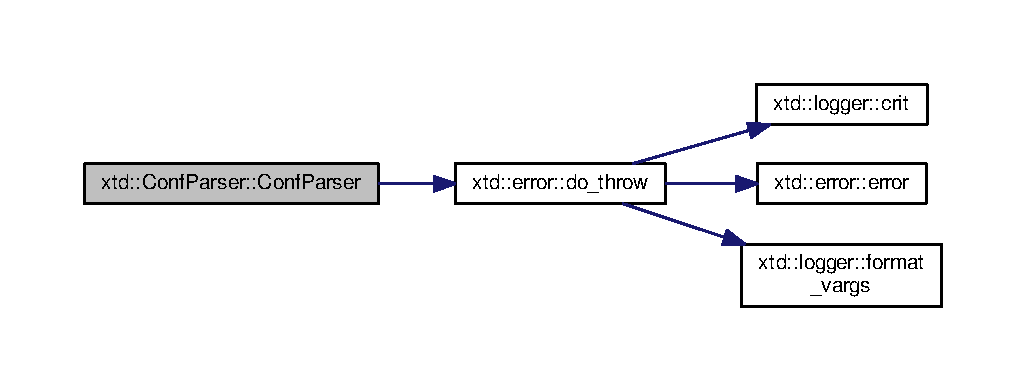
\includegraphics[width=350pt]{classxtd_1_1ConfParser_a5f7729df32b946dba9690494b6fee762_cgraph}
\end{center}
\end{figure}


\hypertarget{classxtd_1_1ConfParser_a460c904cfe815a6141feb088022c9564}{\index{xtd\-::\-Conf\-Parser@{xtd\-::\-Conf\-Parser}!Conf\-Parser@{Conf\-Parser}}
\index{Conf\-Parser@{Conf\-Parser}!xtd::ConfParser@{xtd\-::\-Conf\-Parser}}
\subsubsection[{Conf\-Parser}]{\setlength{\rightskip}{0pt plus 5cm}xtd\-::\-Conf\-Parser\-::\-Conf\-Parser (
\begin{DoxyParamCaption}
\item[{const string \&}]{p\-\_\-path, }
\item[{const {\bf t\-\_\-param\-\_\-map} \&}]{p\-\_\-params}
\end{DoxyParamCaption}
)}}\label{classxtd_1_1ConfParser_a460c904cfe815a6141feb088022c9564}


Definition at line 23 of file Conf\-Parser.\-cc.


\begin{DoxyCode}
24                                                     :
25   \hyperlink{classxtd_1_1ConfParser_a5203f3b8cb6e9070b33371c9acabbc8c}{m\_nblines}(0),
26   \hyperlink{classxtd_1_1ConfParser_abe309999c7964603bde870c7bda16d2e}{m\_paramMap}(p\_params)
27 \{
28   \textcolor{keywordflow}{if} (\hyperlink{namespacextd_a68ed4fe8e9c11116b68efe5b102aec50a444bcb3a3fcf8389296c49467f27e1d6}{status::ok} != initialize(p\_fileName))
29     \hyperlink{classxtd_1_1error_a34fcbd60f169444fa6b9b410db6ddaaf}{error::do\_throw}(\textcolor{stringliteral}{"common.configparser"}, \textcolor{stringliteral}{"could not initialize config from file %s"}, 
      p\_fileName, \hyperlink{logger_8hh_a3fe03e23176f4fe277d1d3b41f3d3d06}{HERE});
30 \}
\end{DoxyCode}


Here is the call graph for this function\-:
\nopagebreak
\begin{figure}[H]
\begin{center}
\leavevmode
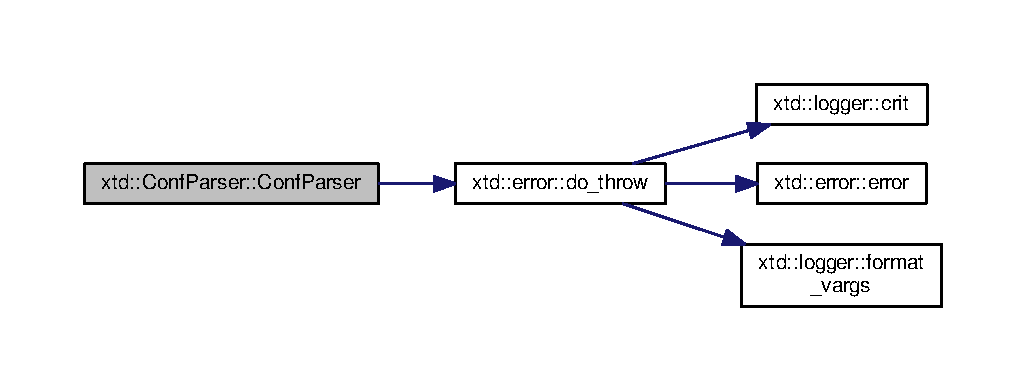
\includegraphics[width=350pt]{classxtd_1_1ConfParser_a460c904cfe815a6141feb088022c9564_cgraph}
\end{center}
\end{figure}




\subsection{Member Function Documentation}
\hypertarget{classxtd_1_1ConfParser_a18fa4083def8aaf86796b9ddbc331daf}{\index{xtd\-::\-Conf\-Parser@{xtd\-::\-Conf\-Parser}!begin@{begin}}
\index{begin@{begin}!xtd::ConfParser@{xtd\-::\-Conf\-Parser}}
\subsubsection[{begin}]{\setlength{\rightskip}{0pt plus 5cm}{\bf Conf\-Parser\-::const\-\_\-iterator} xtd\-::\-Conf\-Parser\-::begin (
\begin{DoxyParamCaption}
\item[{void}]{}
\end{DoxyParamCaption}
) const\hspace{0.3cm}{\ttfamily [inline]}}}\label{classxtd_1_1ConfParser_a18fa4083def8aaf86796b9ddbc331daf}


Definition at line 216 of file Conf\-Parser.\-hh.


\begin{DoxyCode}
217 \{
218   \textcolor{keywordflow}{return} const\_iterator(\hyperlink{classxtd_1_1ConfParser_a100cffb5f33795e50c87ab5fb2a43963}{m\_sections}.begin());
219 \}
\end{DoxyCode}
\hypertarget{classxtd_1_1ConfParser_ae7e7ade9440517b79cc22f21b10df7a5}{\index{xtd\-::\-Conf\-Parser@{xtd\-::\-Conf\-Parser}!dump\-Keys@{dump\-Keys}}
\index{dump\-Keys@{dump\-Keys}!xtd::ConfParser@{xtd\-::\-Conf\-Parser}}
\subsubsection[{dump\-Keys}]{\setlength{\rightskip}{0pt plus 5cm}void xtd\-::\-Conf\-Parser\-::dump\-Keys (
\begin{DoxyParamCaption}
\item[{std\-::ostream \&}]{p\-\_\-stream}
\end{DoxyParamCaption}
) const}}\label{classxtd_1_1ConfParser_ae7e7ade9440517b79cc22f21b10df7a5}
dump all keys found in conf file 
\begin{DoxyParams}{Parameters}
{\em p\-\_\-stream} & output stream \\
\hline
\end{DoxyParams}


Definition at line 610 of file Conf\-Parser.\-cc.


\begin{DoxyCode}
611 \{
612   t\_value\_map::const\_iterator cc\_value;
613 
614   \textcolor{keywordflow}{for} (cc\_value =  \hyperlink{classxtd_1_1ConfParser_a4c58cc4fa96ebaddd180a0c67edb481f}{m\_values}.begin();
615        cc\_value != \hyperlink{classxtd_1_1ConfParser_a4c58cc4fa96ebaddd180a0c67edb481f}{m\_values}.end();
616        cc\_value++)
617   \{
618     p\_stream << \textcolor{stringliteral}{"keys '"} << cc\_value->first
619              << \textcolor{stringliteral}{"' contains '"} << cc\_value->second << \textcolor{stringliteral}{"'"}
620              << std::endl;
621   \}
622 \}
\end{DoxyCode}
\hypertarget{classxtd_1_1ConfParser_ab772ae8e571f1a3f719eca2f9d056d7c}{\index{xtd\-::\-Conf\-Parser@{xtd\-::\-Conf\-Parser}!end@{end}}
\index{end@{end}!xtd::ConfParser@{xtd\-::\-Conf\-Parser}}
\subsubsection[{end}]{\setlength{\rightskip}{0pt plus 5cm}{\bf Conf\-Parser\-::const\-\_\-iterator} xtd\-::\-Conf\-Parser\-::end (
\begin{DoxyParamCaption}
\item[{void}]{}
\end{DoxyParamCaption}
) const\hspace{0.3cm}{\ttfamily [inline]}}}\label{classxtd_1_1ConfParser_ab772ae8e571f1a3f719eca2f9d056d7c}


Definition at line 222 of file Conf\-Parser.\-hh.


\begin{DoxyCode}
223 \{
224   \textcolor{keywordflow}{return} const\_iterator(\hyperlink{classxtd_1_1ConfParser_a100cffb5f33795e50c87ab5fb2a43963}{m\_sections}.end());
225 \}
\end{DoxyCode}
\hypertarget{classxtd_1_1ConfParser_a7f1323a9ef1f85c73a0bff383e24967c}{\index{xtd\-::\-Conf\-Parser@{xtd\-::\-Conf\-Parser}!exists@{exists}}
\index{exists@{exists}!xtd::ConfParser@{xtd\-::\-Conf\-Parser}}
\subsubsection[{exists}]{\setlength{\rightskip}{0pt plus 5cm}bool xtd\-::\-Conf\-Parser\-::exists (
\begin{DoxyParamCaption}
\item[{const string \&}]{p\-\_\-name}
\end{DoxyParamCaption}
) const}}\label{classxtd_1_1ConfParser_a7f1323a9ef1f85c73a0bff383e24967c}


Indique si la clef p\-\_\-name existe dans le fichier de conf. 


\begin{DoxyParams}{Parameters}
{\em p\-\_\-name} & clef à chercher \\
\hline
\end{DoxyParams}
\begin{DoxyReturn}{Returns}
vrai si p\-\_\-name existe, faux sinon 
\end{DoxyReturn}


Definition at line 604 of file Conf\-Parser.\-cc.


\begin{DoxyCode}
605 \{
606   \textcolor{keywordflow}{return} (\hyperlink{classxtd_1_1ConfParser_a4c58cc4fa96ebaddd180a0c67edb481f}{m\_values}.find(p\_name) != \hyperlink{classxtd_1_1ConfParser_a4c58cc4fa96ebaddd180a0c67edb481f}{m\_values}.end());
607 \}
\end{DoxyCode}
\hypertarget{classxtd_1_1ConfParser_a18acbfe7e5828eff045bdcc941626974}{\index{xtd\-::\-Conf\-Parser@{xtd\-::\-Conf\-Parser}!find@{find}}
\index{find@{find}!xtd::ConfParser@{xtd\-::\-Conf\-Parser}}
\subsubsection[{find}]{\setlength{\rightskip}{0pt plus 5cm}{\bf Conf\-Parser\-::const\-\_\-iterator} xtd\-::\-Conf\-Parser\-::find (
\begin{DoxyParamCaption}
\item[{const char $\ast$}]{p\-\_\-name}
\end{DoxyParamCaption}
) const\hspace{0.3cm}{\ttfamily [inline]}}}\label{classxtd_1_1ConfParser_a18acbfe7e5828eff045bdcc941626974}


Definition at line 210 of file Conf\-Parser.\-hh.


\begin{DoxyCode}
211 \{
212   \textcolor{keywordflow}{return} \hyperlink{classxtd_1_1ConfParser_a18acbfe7e5828eff045bdcc941626974}{find}(\textcolor{keywordtype}{string}(p\_name));
213 \}
\end{DoxyCode}
\hypertarget{classxtd_1_1ConfParser_aff7ee8bcd3de4359eff719bc4a6570ba}{\index{xtd\-::\-Conf\-Parser@{xtd\-::\-Conf\-Parser}!find@{find}}
\index{find@{find}!xtd::ConfParser@{xtd\-::\-Conf\-Parser}}
\subsubsection[{find}]{\setlength{\rightskip}{0pt plus 5cm}{\bf Conf\-Parser\-::const\-\_\-iterator} xtd\-::\-Conf\-Parser\-::find (
\begin{DoxyParamCaption}
\item[{const string \&}]{p\-\_\-key}
\end{DoxyParamCaption}
) const\hspace{0.3cm}{\ttfamily [inline]}}}\label{classxtd_1_1ConfParser_aff7ee8bcd3de4359eff719bc4a6570ba}


Definition at line 201 of file Conf\-Parser.\-hh.


\begin{DoxyCode}
202 \{
203   const\_iterator cc\_result =
204     std::find\_if(\hyperlink{classxtd_1_1ConfParser_a100cffb5f33795e50c87ab5fb2a43963}{m\_sections}.begin(), \hyperlink{classxtd_1_1ConfParser_a100cffb5f33795e50c87ab5fb2a43963}{m\_sections}.end(),
205                  boost::bind(&t\_section\_data::first, \_1) == p\_key);
206   \textcolor{keywordflow}{return} cc\_result;
207 \}
\end{DoxyCode}
\hypertarget{classxtd_1_1ConfParser_a5ef18d8778c844ce60f2c93579be7926}{\index{xtd\-::\-Conf\-Parser@{xtd\-::\-Conf\-Parser}!get@{get}}
\index{get@{get}!xtd::ConfParser@{xtd\-::\-Conf\-Parser}}
\subsubsection[{get}]{\setlength{\rightskip}{0pt plus 5cm}{\bf status} xtd\-::\-Conf\-Parser\-::get (
\begin{DoxyParamCaption}
\item[{const string \&}]{p\-\_\-name, }
\item[{string \&}]{p\-\_\-dval}
\end{DoxyParamCaption}
) const}}\label{classxtd_1_1ConfParser_a5ef18d8778c844ce60f2c93579be7926}


Definition at line 405 of file Conf\-Parser.\-cc.


\begin{DoxyCode}
406 \{
407   t\_value\_map::const\_iterator cc\_value;
408 
409   \textcolor{keywordflow}{if} ((cc\_value = \hyperlink{classxtd_1_1ConfParser_a4c58cc4fa96ebaddd180a0c67edb481f}{m\_values}.find(p\_name)) == \hyperlink{classxtd_1_1ConfParser_a4c58cc4fa96ebaddd180a0c67edb481f}{m\_values}.end())
410   \{
411     \hyperlink{classxtd_1_1logger_ac6cf4c5d929c844041ea9763cc3926be}{logger::info}(\textcolor{stringliteral}{"common.confparser"}, \textcolor{stringliteral}{"key '%s' not found in conf file '%s'"}, p\_name, 
      \hyperlink{classxtd_1_1ConfParser_abc9e0b073f91de77b76db39bfbc27508}{m\_filename}, \hyperlink{logger_8hh_a3fe03e23176f4fe277d1d3b41f3d3d06}{HERE});
412     \textcolor{keywordflow}{return} \hyperlink{namespacextd_a68ed4fe8e9c11116b68efe5b102aec50acb5e100e5a9a3e7f6d1fd97512215282}{status::error};
413   \}
414 
415   p\_val = cc\_value->second;
416   \textcolor{keywordflow}{return} \hyperlink{namespacextd_a68ed4fe8e9c11116b68efe5b102aec50a444bcb3a3fcf8389296c49467f27e1d6}{status::ok};
417 \}
\end{DoxyCode}


Here is the call graph for this function\-:
\nopagebreak
\begin{figure}[H]
\begin{center}
\leavevmode
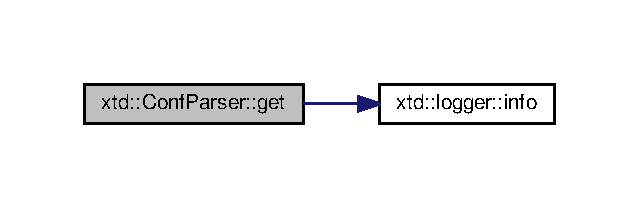
\includegraphics[width=306pt]{classxtd_1_1ConfParser_a5ef18d8778c844ce60f2c93579be7926_cgraph}
\end{center}
\end{figure}


\hypertarget{classxtd_1_1ConfParser_ac8f46e56cdd5d015719c682707b12bc2}{\index{xtd\-::\-Conf\-Parser@{xtd\-::\-Conf\-Parser}!get@{get}}
\index{get@{get}!xtd::ConfParser@{xtd\-::\-Conf\-Parser}}
\subsubsection[{get}]{\setlength{\rightskip}{0pt plus 5cm}{\bf status} xtd\-::\-Conf\-Parser\-::get (
\begin{DoxyParamCaption}
\item[{const string \&}]{p\-\_\-name, }
\item[{const char $\ast$\&}]{p\-\_\-dval}
\end{DoxyParamCaption}
) const}}\label{classxtd_1_1ConfParser_ac8f46e56cdd5d015719c682707b12bc2}


Definition at line 389 of file Conf\-Parser.\-cc.


\begin{DoxyCode}
390 \{
391   t\_value\_map::const\_iterator cc\_value;
392 
393   \textcolor{keywordflow}{if} ((cc\_value = \hyperlink{classxtd_1_1ConfParser_a4c58cc4fa96ebaddd180a0c67edb481f}{m\_values}.find(p\_name)) == \hyperlink{classxtd_1_1ConfParser_a4c58cc4fa96ebaddd180a0c67edb481f}{m\_values}.end())
394   \{
395     \hyperlink{classxtd_1_1logger_ac6cf4c5d929c844041ea9763cc3926be}{logger::info}(\textcolor{stringliteral}{"common.confparser"}, \textcolor{stringliteral}{"key '%s' not found in conf file '%s'"}, p\_name, 
      \hyperlink{classxtd_1_1ConfParser_abc9e0b073f91de77b76db39bfbc27508}{m\_filename}, \hyperlink{logger_8hh_a3fe03e23176f4fe277d1d3b41f3d3d06}{HERE});
396     \textcolor{keywordflow}{return} \hyperlink{namespacextd_a68ed4fe8e9c11116b68efe5b102aec50acb5e100e5a9a3e7f6d1fd97512215282}{status::error};
397   \}
398 
399   p\_val = cc\_value->second.c\_str();
400   \textcolor{keywordflow}{return} \hyperlink{namespacextd_a68ed4fe8e9c11116b68efe5b102aec50a444bcb3a3fcf8389296c49467f27e1d6}{status::ok};
401 \}
\end{DoxyCode}


Here is the call graph for this function\-:
\nopagebreak
\begin{figure}[H]
\begin{center}
\leavevmode
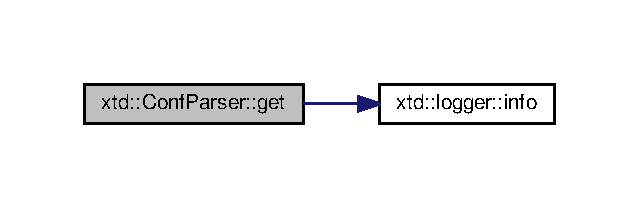
\includegraphics[width=306pt]{classxtd_1_1ConfParser_ac8f46e56cdd5d015719c682707b12bc2_cgraph}
\end{center}
\end{figure}


\hypertarget{classxtd_1_1ConfParser_adaf860ed87b32df2ac16f73cab8bbbed}{\index{xtd\-::\-Conf\-Parser@{xtd\-::\-Conf\-Parser}!get@{get}}
\index{get@{get}!xtd::ConfParser@{xtd\-::\-Conf\-Parser}}
\subsubsection[{get}]{\setlength{\rightskip}{0pt plus 5cm}{\bf status} xtd\-::\-Conf\-Parser\-::get (
\begin{DoxyParamCaption}
\item[{const string \&}]{p\-\_\-name, }
\item[{char \&}]{p\-\_\-ival}
\end{DoxyParamCaption}
) const}}\label{classxtd_1_1ConfParser_adaf860ed87b32df2ac16f73cab8bbbed}


Definition at line 422 of file Conf\-Parser.\-cc.


\begin{DoxyCode}
423 \{
424   \textcolor{keywordtype}{string} l\_value;
425 
426   \textcolor{keywordflow}{if} (\hyperlink{namespacextd_a68ed4fe8e9c11116b68efe5b102aec50a444bcb3a3fcf8389296c49467f27e1d6}{status::ok} != \textcolor{keyword}{get}(p\_name, l\_value))
427     \textcolor{keywordflow}{return} \hyperlink{namespacextd_a68ed4fe8e9c11116b68efe5b102aec50acb5e100e5a9a3e7f6d1fd97512215282}{status::error};
428 
429   p\_val = atoi(l\_value.c\_str());
430 
431   \textcolor{keywordflow}{if} (errno == ERANGE)
432     \textcolor{keywordflow}{return} \hyperlink{namespacextd_a68ed4fe8e9c11116b68efe5b102aec50acb5e100e5a9a3e7f6d1fd97512215282}{status::error};
433   \textcolor{keywordflow}{return} \hyperlink{namespacextd_a68ed4fe8e9c11116b68efe5b102aec50a444bcb3a3fcf8389296c49467f27e1d6}{status::ok};
434 \}
\end{DoxyCode}
\hypertarget{classxtd_1_1ConfParser_a6edfffe778ba93a7dc0ce3b71e1a293d}{\index{xtd\-::\-Conf\-Parser@{xtd\-::\-Conf\-Parser}!get@{get}}
\index{get@{get}!xtd::ConfParser@{xtd\-::\-Conf\-Parser}}
\subsubsection[{get}]{\setlength{\rightskip}{0pt plus 5cm}{\bf status} xtd\-::\-Conf\-Parser\-::get (
\begin{DoxyParamCaption}
\item[{const string \&}]{p\-\_\-name, }
\item[{unsigned char \&}]{p\-\_\-ival}
\end{DoxyParamCaption}
) const}}\label{classxtd_1_1ConfParser_a6edfffe778ba93a7dc0ce3b71e1a293d}


Definition at line 437 of file Conf\-Parser.\-cc.


\begin{DoxyCode}
438 \{
439   \textcolor{keywordtype}{string} l\_value;
440 
441   \textcolor{keywordflow}{if} (\hyperlink{namespacextd_a68ed4fe8e9c11116b68efe5b102aec50a444bcb3a3fcf8389296c49467f27e1d6}{status::ok} != \textcolor{keyword}{get}(p\_name, l\_value))
442     \textcolor{keywordflow}{return} \hyperlink{namespacextd_a68ed4fe8e9c11116b68efe5b102aec50acb5e100e5a9a3e7f6d1fd97512215282}{status::error};
443 
444   p\_val = atoi(l\_value.c\_str());
445   \textcolor{keywordflow}{if} (errno == ERANGE)
446     \textcolor{keywordflow}{return} \hyperlink{namespacextd_a68ed4fe8e9c11116b68efe5b102aec50acb5e100e5a9a3e7f6d1fd97512215282}{status::error};
447 
448   \textcolor{keywordflow}{return} \hyperlink{namespacextd_a68ed4fe8e9c11116b68efe5b102aec50a444bcb3a3fcf8389296c49467f27e1d6}{status::ok};
449 \}
\end{DoxyCode}
\hypertarget{classxtd_1_1ConfParser_abd0bb9c9e8568c0b2dd28b133f700681}{\index{xtd\-::\-Conf\-Parser@{xtd\-::\-Conf\-Parser}!get@{get}}
\index{get@{get}!xtd::ConfParser@{xtd\-::\-Conf\-Parser}}
\subsubsection[{get}]{\setlength{\rightskip}{0pt plus 5cm}{\bf status} xtd\-::\-Conf\-Parser\-::get (
\begin{DoxyParamCaption}
\item[{const string \&}]{p\-\_\-name, }
\item[{unsigned short \&}]{p\-\_\-ival}
\end{DoxyParamCaption}
) const}}\label{classxtd_1_1ConfParser_abd0bb9c9e8568c0b2dd28b133f700681}


Definition at line 452 of file Conf\-Parser.\-cc.


\begin{DoxyCode}
453 \{
454   \textcolor{keywordtype}{string} l\_value;
455 
456   \textcolor{keywordflow}{if} (\hyperlink{namespacextd_a68ed4fe8e9c11116b68efe5b102aec50a444bcb3a3fcf8389296c49467f27e1d6}{status::ok} != \textcolor{keyword}{get}(p\_name, l\_value))
457     \textcolor{keywordflow}{return} \hyperlink{namespacextd_a68ed4fe8e9c11116b68efe5b102aec50acb5e100e5a9a3e7f6d1fd97512215282}{status::error};
458 
459   p\_val = atoi(l\_value.c\_str());
460 
461   \textcolor{keywordflow}{if} (errno == ERANGE)
462     \textcolor{keywordflow}{return} \hyperlink{namespacextd_a68ed4fe8e9c11116b68efe5b102aec50acb5e100e5a9a3e7f6d1fd97512215282}{status::error} ;
463   \textcolor{keywordflow}{return} \hyperlink{namespacextd_a68ed4fe8e9c11116b68efe5b102aec50a444bcb3a3fcf8389296c49467f27e1d6}{status::ok} ;
464 \}
\end{DoxyCode}
\hypertarget{classxtd_1_1ConfParser_a902dfe3ab82e8d1710659f65fa0e853b}{\index{xtd\-::\-Conf\-Parser@{xtd\-::\-Conf\-Parser}!get@{get}}
\index{get@{get}!xtd::ConfParser@{xtd\-::\-Conf\-Parser}}
\subsubsection[{get}]{\setlength{\rightskip}{0pt plus 5cm}{\bf status} xtd\-::\-Conf\-Parser\-::get (
\begin{DoxyParamCaption}
\item[{const string \&}]{p\-\_\-name, }
\item[{int \&}]{p\-\_\-ival}
\end{DoxyParamCaption}
) const}}\label{classxtd_1_1ConfParser_a902dfe3ab82e8d1710659f65fa0e853b}


Definition at line 468 of file Conf\-Parser.\-cc.


\begin{DoxyCode}
469 \{
470   \textcolor{keywordtype}{string} l\_value;
471 
472   \textcolor{keywordflow}{if} (\hyperlink{namespacextd_a68ed4fe8e9c11116b68efe5b102aec50a444bcb3a3fcf8389296c49467f27e1d6}{status::ok} != \textcolor{keyword}{get}(p\_name, l\_value))
473     \textcolor{keywordflow}{return} \hyperlink{namespacextd_a68ed4fe8e9c11116b68efe5b102aec50acb5e100e5a9a3e7f6d1fd97512215282}{status::error};
474 
475   p\_val = atoi(l\_value.c\_str());
476 
477   \textcolor{keywordflow}{if} (errno == ERANGE)
478     \textcolor{keywordflow}{return} \hyperlink{namespacextd_a68ed4fe8e9c11116b68efe5b102aec50acb5e100e5a9a3e7f6d1fd97512215282}{status::error} ;
479   \textcolor{keywordflow}{return} \hyperlink{namespacextd_a68ed4fe8e9c11116b68efe5b102aec50a444bcb3a3fcf8389296c49467f27e1d6}{status::ok} ;
480 \}
\end{DoxyCode}
\hypertarget{classxtd_1_1ConfParser_aeabbb63eeeafaf9d0853fdcf5b2a83eb}{\index{xtd\-::\-Conf\-Parser@{xtd\-::\-Conf\-Parser}!get@{get}}
\index{get@{get}!xtd::ConfParser@{xtd\-::\-Conf\-Parser}}
\subsubsection[{get}]{\setlength{\rightskip}{0pt plus 5cm}{\bf status} xtd\-::\-Conf\-Parser\-::get (
\begin{DoxyParamCaption}
\item[{const string \&}]{p\-\_\-name, }
\item[{long \&}]{p\-\_\-ival}
\end{DoxyParamCaption}
) const}}\label{classxtd_1_1ConfParser_aeabbb63eeeafaf9d0853fdcf5b2a83eb}


Definition at line 484 of file Conf\-Parser.\-cc.


\begin{DoxyCode}
485 \{
486   \textcolor{keywordtype}{string} l\_value;
487 
488   \textcolor{keywordflow}{if} (\hyperlink{namespacextd_a68ed4fe8e9c11116b68efe5b102aec50a444bcb3a3fcf8389296c49467f27e1d6}{status::ok} != \textcolor{keyword}{get}(p\_name, l\_value))
489     \textcolor{keywordflow}{return} \hyperlink{namespacextd_a68ed4fe8e9c11116b68efe5b102aec50acb5e100e5a9a3e7f6d1fd97512215282}{status::error};
490 
491   p\_val = strtol(l\_value.c\_str(), NULL, 10);
492 
493   \textcolor{keywordflow}{if} (errno == ERANGE)
494     \textcolor{keywordflow}{return} \hyperlink{namespacextd_a68ed4fe8e9c11116b68efe5b102aec50acb5e100e5a9a3e7f6d1fd97512215282}{status::error} ;
495   \textcolor{keywordflow}{return} \hyperlink{namespacextd_a68ed4fe8e9c11116b68efe5b102aec50a444bcb3a3fcf8389296c49467f27e1d6}{status::ok} ;
496 \}
\end{DoxyCode}
\hypertarget{classxtd_1_1ConfParser_a38c007fd9a93cf370a9e2de14e021faf}{\index{xtd\-::\-Conf\-Parser@{xtd\-::\-Conf\-Parser}!get@{get}}
\index{get@{get}!xtd::ConfParser@{xtd\-::\-Conf\-Parser}}
\subsubsection[{get}]{\setlength{\rightskip}{0pt plus 5cm}{\bf status} xtd\-::\-Conf\-Parser\-::get (
\begin{DoxyParamCaption}
\item[{const string \&}]{p\-\_\-name, }
\item[{unsigned long long \&}]{p\-\_\-ival}
\end{DoxyParamCaption}
) const}}\label{classxtd_1_1ConfParser_a38c007fd9a93cf370a9e2de14e021faf}


Definition at line 499 of file Conf\-Parser.\-cc.


\begin{DoxyCode}
500 \{
501   \textcolor{keywordtype}{string} l\_value;
502 
503   \textcolor{keywordflow}{if} (\hyperlink{namespacextd_a68ed4fe8e9c11116b68efe5b102aec50a444bcb3a3fcf8389296c49467f27e1d6}{status::ok} != \textcolor{keyword}{get}(p\_name, l\_value))
504     \textcolor{keywordflow}{return} \hyperlink{namespacextd_a68ed4fe8e9c11116b68efe5b102aec50acb5e100e5a9a3e7f6d1fd97512215282}{status::error};
505 
506   p\_val = strtoull(l\_value.c\_str(), NULL, 10);
507 
508   \textcolor{keywordflow}{if} (errno == ERANGE)
509     \textcolor{keywordflow}{return} \hyperlink{namespacextd_a68ed4fe8e9c11116b68efe5b102aec50acb5e100e5a9a3e7f6d1fd97512215282}{status::error} ;
510   \textcolor{keywordflow}{return} \hyperlink{namespacextd_a68ed4fe8e9c11116b68efe5b102aec50a444bcb3a3fcf8389296c49467f27e1d6}{status::ok} ;
511 \}
\end{DoxyCode}
\hypertarget{classxtd_1_1ConfParser_a39e678dc0205b82f4cce76533f4f4d84}{\index{xtd\-::\-Conf\-Parser@{xtd\-::\-Conf\-Parser}!get@{get}}
\index{get@{get}!xtd::ConfParser@{xtd\-::\-Conf\-Parser}}
\subsubsection[{get}]{\setlength{\rightskip}{0pt plus 5cm}{\bf status} xtd\-::\-Conf\-Parser\-::get (
\begin{DoxyParamCaption}
\item[{const string \&}]{p\-\_\-name, }
\item[{unsigned long \&}]{p\-\_\-ival}
\end{DoxyParamCaption}
) const}}\label{classxtd_1_1ConfParser_a39e678dc0205b82f4cce76533f4f4d84}


Definition at line 514 of file Conf\-Parser.\-cc.


\begin{DoxyCode}
515 \{
516   \textcolor{keywordtype}{string} l\_value;
517 
518   \textcolor{keywordflow}{if} (\hyperlink{namespacextd_a68ed4fe8e9c11116b68efe5b102aec50a444bcb3a3fcf8389296c49467f27e1d6}{status::ok} != \textcolor{keyword}{get}(p\_name, l\_value))
519     \textcolor{keywordflow}{return} \hyperlink{namespacextd_a68ed4fe8e9c11116b68efe5b102aec50acb5e100e5a9a3e7f6d1fd97512215282}{status::error};
520 
521   p\_val = strtoul(l\_value.c\_str(), NULL, 10);
522 
523   \textcolor{keywordflow}{if} (errno == ERANGE)
524     \textcolor{keywordflow}{return} \hyperlink{namespacextd_a68ed4fe8e9c11116b68efe5b102aec50acb5e100e5a9a3e7f6d1fd97512215282}{status::error} ;
525   \textcolor{keywordflow}{return} \hyperlink{namespacextd_a68ed4fe8e9c11116b68efe5b102aec50a444bcb3a3fcf8389296c49467f27e1d6}{status::ok} ;
526 \}
\end{DoxyCode}
\hypertarget{classxtd_1_1ConfParser_a1e8fd9399881ef9910fd144377ff4c93}{\index{xtd\-::\-Conf\-Parser@{xtd\-::\-Conf\-Parser}!get@{get}}
\index{get@{get}!xtd::ConfParser@{xtd\-::\-Conf\-Parser}}
\subsubsection[{get}]{\setlength{\rightskip}{0pt plus 5cm}{\bf status} xtd\-::\-Conf\-Parser\-::get (
\begin{DoxyParamCaption}
\item[{const string \&}]{p\-\_\-name, }
\item[{unsigned int \&}]{p\-\_\-ival}
\end{DoxyParamCaption}
) const}}\label{classxtd_1_1ConfParser_a1e8fd9399881ef9910fd144377ff4c93}


Definition at line 531 of file Conf\-Parser.\-cc.


\begin{DoxyCode}
532 \{
533   \textcolor{keywordtype}{string} l\_value;
534 
535   \textcolor{keywordflow}{if} (\hyperlink{namespacextd_a68ed4fe8e9c11116b68efe5b102aec50a444bcb3a3fcf8389296c49467f27e1d6}{status::ok} != \textcolor{keyword}{get}(p\_name, l\_value))
536     \textcolor{keywordflow}{return} \hyperlink{namespacextd_a68ed4fe8e9c11116b68efe5b102aec50acb5e100e5a9a3e7f6d1fd97512215282}{status::error};
537 
538   p\_val = strtol(l\_value.c\_str(), NULL, 10);
539 
540   \textcolor{keywordflow}{if} (errno == ERANGE)
541     \textcolor{keywordflow}{return} \hyperlink{namespacextd_a68ed4fe8e9c11116b68efe5b102aec50acb5e100e5a9a3e7f6d1fd97512215282}{status::error} ;
542   \textcolor{keywordflow}{return} \hyperlink{namespacextd_a68ed4fe8e9c11116b68efe5b102aec50a444bcb3a3fcf8389296c49467f27e1d6}{status::ok} ;
543 \}
\end{DoxyCode}
\hypertarget{classxtd_1_1ConfParser_a6d091368a02f05c377c7d27d748b64be}{\index{xtd\-::\-Conf\-Parser@{xtd\-::\-Conf\-Parser}!get@{get}}
\index{get@{get}!xtd::ConfParser@{xtd\-::\-Conf\-Parser}}
\subsubsection[{get}]{\setlength{\rightskip}{0pt plus 5cm}{\bf status} xtd\-::\-Conf\-Parser\-::get (
\begin{DoxyParamCaption}
\item[{const string \&}]{p\-\_\-name, }
\item[{double \&}]{p\-\_\-dval}
\end{DoxyParamCaption}
) const}}\label{classxtd_1_1ConfParser_a6d091368a02f05c377c7d27d748b64be}


Definition at line 547 of file Conf\-Parser.\-cc.


\begin{DoxyCode}
548 \{
549   \textcolor{keywordtype}{string} l\_value;
550 
551   \textcolor{keywordflow}{if} (\hyperlink{namespacextd_a68ed4fe8e9c11116b68efe5b102aec50a444bcb3a3fcf8389296c49467f27e1d6}{status::ok} != \textcolor{keyword}{get}(p\_name, l\_value))
552     \textcolor{keywordflow}{return} \hyperlink{namespacextd_a68ed4fe8e9c11116b68efe5b102aec50acb5e100e5a9a3e7f6d1fd97512215282}{status::error};
553 
554   p\_val = strtod(l\_value.c\_str(), NULL);
555 
556   \textcolor{keywordflow}{if} (errno == ERANGE)
557     \textcolor{keywordflow}{return} \hyperlink{namespacextd_a68ed4fe8e9c11116b68efe5b102aec50acb5e100e5a9a3e7f6d1fd97512215282}{status::error} ;
558   \textcolor{keywordflow}{return} \hyperlink{namespacextd_a68ed4fe8e9c11116b68efe5b102aec50a444bcb3a3fcf8389296c49467f27e1d6}{status::ok} ;
559 \}
\end{DoxyCode}
\hypertarget{classxtd_1_1ConfParser_ac0d9efc31b6b6989f4a9f6061ad03596}{\index{xtd\-::\-Conf\-Parser@{xtd\-::\-Conf\-Parser}!get@{get}}
\index{get@{get}!xtd::ConfParser@{xtd\-::\-Conf\-Parser}}
\subsubsection[{get}]{\setlength{\rightskip}{0pt plus 5cm}{\bf status} xtd\-::\-Conf\-Parser\-::get (
\begin{DoxyParamCaption}
\item[{const string \&}]{p\-\_\-name, }
\item[{float \&}]{p\-\_\-dval}
\end{DoxyParamCaption}
) const}}\label{classxtd_1_1ConfParser_ac0d9efc31b6b6989f4a9f6061ad03596}


Definition at line 563 of file Conf\-Parser.\-cc.


\begin{DoxyCode}
564 \{
565   \textcolor{keywordtype}{string} l\_value;
566 
567   \textcolor{keywordflow}{if} (\hyperlink{namespacextd_a68ed4fe8e9c11116b68efe5b102aec50a444bcb3a3fcf8389296c49467f27e1d6}{status::ok} != \textcolor{keyword}{get}(p\_name, l\_value))
568     \textcolor{keywordflow}{return} \hyperlink{namespacextd_a68ed4fe8e9c11116b68efe5b102aec50acb5e100e5a9a3e7f6d1fd97512215282}{status::error};
569 
570   p\_val = strtof(l\_value.c\_str(), NULL);
571 
572   \textcolor{keywordflow}{if} (errno == ERANGE)
573     \textcolor{keywordflow}{return} \hyperlink{namespacextd_a68ed4fe8e9c11116b68efe5b102aec50acb5e100e5a9a3e7f6d1fd97512215282}{status::error};
574   \textcolor{keywordflow}{return} \hyperlink{namespacextd_a68ed4fe8e9c11116b68efe5b102aec50a444bcb3a3fcf8389296c49467f27e1d6}{status::ok};
575 \}
\end{DoxyCode}
\hypertarget{classxtd_1_1ConfParser_a8a8e729b8e11c5efd19dec29baa31f66}{\index{xtd\-::\-Conf\-Parser@{xtd\-::\-Conf\-Parser}!get@{get}}
\index{get@{get}!xtd::ConfParser@{xtd\-::\-Conf\-Parser}}
\subsubsection[{get}]{\setlength{\rightskip}{0pt plus 5cm}{\bf status} xtd\-::\-Conf\-Parser\-::get (
\begin{DoxyParamCaption}
\item[{const string \&}]{p\-\_\-name, }
\item[{bool \&}]{p\-\_\-dval}
\end{DoxyParamCaption}
) const}}\label{classxtd_1_1ConfParser_a8a8e729b8e11c5efd19dec29baa31f66}


Definition at line 579 of file Conf\-Parser.\-cc.


\begin{DoxyCode}
580 \{
581   \textcolor{keywordtype}{string} l\_value;
582 
583   \textcolor{keywordflow}{if} (\hyperlink{namespacextd_a68ed4fe8e9c11116b68efe5b102aec50a444bcb3a3fcf8389296c49467f27e1d6}{status::ok} != \textcolor{keyword}{get}(p\_name, l\_value))
584     \textcolor{keywordflow}{return} \hyperlink{namespacextd_a68ed4fe8e9c11116b68efe5b102aec50acb5e100e5a9a3e7f6d1fd97512215282}{status::error} ;
585 
586   boost::trim(l\_value);
587   boost::to\_lower(l\_value);
588 
589   \textcolor{keywordflow}{if} ((\textcolor{stringliteral}{"0"} == l\_value) || (\textcolor{stringliteral}{"no"} == l\_value) || (\textcolor{stringliteral}{"false"} == l\_value))
590   \{
591     p\_val = \textcolor{keyword}{false};
592     \textcolor{keywordflow}{return} \hyperlink{namespacextd_a68ed4fe8e9c11116b68efe5b102aec50a444bcb3a3fcf8389296c49467f27e1d6}{status::ok};
593   \}
594 
595   \textcolor{keywordflow}{if} ((\textcolor{stringliteral}{"1"} == l\_value) || (\textcolor{stringliteral}{"yes"} == l\_value) || (\textcolor{stringliteral}{"true"} == l\_value))
596   \{
597     p\_val = \textcolor{keyword}{true};
598     \textcolor{keywordflow}{return} \hyperlink{namespacextd_a68ed4fe8e9c11116b68efe5b102aec50a444bcb3a3fcf8389296c49467f27e1d6}{status::ok};
599   \}
600   \textcolor{keywordflow}{return} \hyperlink{namespacextd_a68ed4fe8e9c11116b68efe5b102aec50acb5e100e5a9a3e7f6d1fd97512215282}{status::error};
601 \}
\end{DoxyCode}
\hypertarget{classxtd_1_1ConfParser_aa3a209f68c61547141194a305049eeae}{\index{xtd\-::\-Conf\-Parser@{xtd\-::\-Conf\-Parser}!get\-\_\-default@{get\-\_\-default}}
\index{get\-\_\-default@{get\-\_\-default}!xtd::ConfParser@{xtd\-::\-Conf\-Parser}}
\subsubsection[{get\-\_\-default}]{\setlength{\rightskip}{0pt plus 5cm}template$<$typename T $>$ {\bf status} xtd\-::\-Conf\-Parser\-::get\-\_\-default (
\begin{DoxyParamCaption}
\item[{const string \&}]{p\-\_\-key, }
\item[{T \&}]{p\-\_\-dest, }
\item[{const T \&}]{p\-\_\-default}
\end{DoxyParamCaption}
)\hspace{0.3cm}{\ttfamily [inline]}}}\label{classxtd_1_1ConfParser_aa3a209f68c61547141194a305049eeae}


Definition at line 83 of file Conf\-Parser.\-hh.


\begin{DoxyCode}
84   \{
85     \textcolor{keywordflow}{if} (\hyperlink{namespacextd_a68ed4fe8e9c11116b68efe5b102aec50a444bcb3a3fcf8389296c49467f27e1d6}{status::ok} != \textcolor{keyword}{get}(p\_key, p\_dest))
86     \{
87       p\_dest = p\_default;
88       \textcolor{keywordflow}{return} \hyperlink{namespacextd_a68ed4fe8e9c11116b68efe5b102aec50ac2adf6ecc220f2711801d6e466340183}{status::notfound};
89     \}
90     \textcolor{keywordflow}{return} \hyperlink{namespacextd_a68ed4fe8e9c11116b68efe5b102aec50a444bcb3a3fcf8389296c49467f27e1d6}{status::ok};
91   \}
\end{DoxyCode}
\hypertarget{classxtd_1_1ConfParser_a2a72cefc513e103b86d90785862c620f}{\index{xtd\-::\-Conf\-Parser@{xtd\-::\-Conf\-Parser}!get\-File\-Path@{get\-File\-Path}}
\index{get\-File\-Path@{get\-File\-Path}!xtd::ConfParser@{xtd\-::\-Conf\-Parser}}
\subsubsection[{get\-File\-Path}]{\setlength{\rightskip}{0pt plus 5cm}const string \& xtd\-::\-Conf\-Parser\-::get\-File\-Path (
\begin{DoxyParamCaption}
\item[{void}]{}
\end{DoxyParamCaption}
) const\hspace{0.3cm}{\ttfamily [inline]}}}\label{classxtd_1_1ConfParser_a2a72cefc513e103b86d90785862c620f}


Definition at line 195 of file Conf\-Parser.\-hh.


\begin{DoxyCode}
196 \{
197   \textcolor{keywordflow}{return} \hyperlink{classxtd_1_1ConfParser_abc9e0b073f91de77b76db39bfbc27508}{m\_filename};
198 \}
\end{DoxyCode}
\hypertarget{classxtd_1_1ConfParser_a1be1c2813abf959d85bb6cf695c74dec}{\index{xtd\-::\-Conf\-Parser@{xtd\-::\-Conf\-Parser}!get\-Param\-Map@{get\-Param\-Map}}
\index{get\-Param\-Map@{get\-Param\-Map}!xtd::ConfParser@{xtd\-::\-Conf\-Parser}}
\subsubsection[{get\-Param\-Map}]{\setlength{\rightskip}{0pt plus 5cm}const {\bf Conf\-Parser\-::t\-\_\-param\-\_\-map} \& xtd\-::\-Conf\-Parser\-::get\-Param\-Map (
\begin{DoxyParamCaption}
\item[{void}]{}
\end{DoxyParamCaption}
) const}}\label{classxtd_1_1ConfParser_a1be1c2813abf959d85bb6cf695c74dec}


Definition at line 625 of file Conf\-Parser.\-cc.


\begin{DoxyCode}
626 \{
627   \textcolor{keywordflow}{return} \hyperlink{classxtd_1_1ConfParser_a4c58cc4fa96ebaddd180a0c67edb481f}{m\_values};
628 \}
\end{DoxyCode}
\hypertarget{classxtd_1_1ConfParser_a34d7366228341b5501bfec94607dd396}{\index{xtd\-::\-Conf\-Parser@{xtd\-::\-Conf\-Parser}!get\-Value\-Map@{get\-Value\-Map}}
\index{get\-Value\-Map@{get\-Value\-Map}!xtd::ConfParser@{xtd\-::\-Conf\-Parser}}
\subsubsection[{get\-Value\-Map}]{\setlength{\rightskip}{0pt plus 5cm}const Conf\-Parser\-::t\-\_\-value\-\_\-map \& xtd\-::\-Conf\-Parser\-::get\-Value\-Map (
\begin{DoxyParamCaption}
\item[{void}]{}
\end{DoxyParamCaption}
) const\hspace{0.3cm}{\ttfamily [inline]}}}\label{classxtd_1_1ConfParser_a34d7366228341b5501bfec94607dd396}


Definition at line 133 of file Conf\-Parser.\-hh.


\begin{DoxyCode}
134 \{
135   \textcolor{keywordflow}{return} \hyperlink{classxtd_1_1ConfParser_a4c58cc4fa96ebaddd180a0c67edb481f}{m\_values};
136 \}
\end{DoxyCode}


\subsection{Member Data Documentation}
\hypertarget{classxtd_1_1ConfParser_abc9e0b073f91de77b76db39bfbc27508}{\index{xtd\-::\-Conf\-Parser@{xtd\-::\-Conf\-Parser}!m\-\_\-filename@{m\-\_\-filename}}
\index{m\-\_\-filename@{m\-\_\-filename}!xtd::ConfParser@{xtd\-::\-Conf\-Parser}}
\subsubsection[{m\-\_\-filename}]{\setlength{\rightskip}{0pt plus 5cm}string xtd\-::\-Conf\-Parser\-::m\-\_\-filename\hspace{0.3cm}{\ttfamily [protected]}}}\label{classxtd_1_1ConfParser_abc9e0b073f91de77b76db39bfbc27508}


Definition at line 127 of file Conf\-Parser.\-hh.

\hypertarget{classxtd_1_1ConfParser_a5203f3b8cb6e9070b33371c9acabbc8c}{\index{xtd\-::\-Conf\-Parser@{xtd\-::\-Conf\-Parser}!m\-\_\-nblines@{m\-\_\-nblines}}
\index{m\-\_\-nblines@{m\-\_\-nblines}!xtd::ConfParser@{xtd\-::\-Conf\-Parser}}
\subsubsection[{m\-\_\-nblines}]{\setlength{\rightskip}{0pt plus 5cm}int xtd\-::\-Conf\-Parser\-::m\-\_\-nblines\hspace{0.3cm}{\ttfamily [protected]}}}\label{classxtd_1_1ConfParser_a5203f3b8cb6e9070b33371c9acabbc8c}


Definition at line 126 of file Conf\-Parser.\-hh.

\hypertarget{classxtd_1_1ConfParser_abe309999c7964603bde870c7bda16d2e}{\index{xtd\-::\-Conf\-Parser@{xtd\-::\-Conf\-Parser}!m\-\_\-param\-Map@{m\-\_\-param\-Map}}
\index{m\-\_\-param\-Map@{m\-\_\-param\-Map}!xtd::ConfParser@{xtd\-::\-Conf\-Parser}}
\subsubsection[{m\-\_\-param\-Map}]{\setlength{\rightskip}{0pt plus 5cm}{\bf t\-\_\-param\-\_\-map} xtd\-::\-Conf\-Parser\-::m\-\_\-param\-Map\hspace{0.3cm}{\ttfamily [protected]}}}\label{classxtd_1_1ConfParser_abe309999c7964603bde870c7bda16d2e}


Definition at line 128 of file Conf\-Parser.\-hh.

\hypertarget{classxtd_1_1ConfParser_a100cffb5f33795e50c87ab5fb2a43963}{\index{xtd\-::\-Conf\-Parser@{xtd\-::\-Conf\-Parser}!m\-\_\-sections@{m\-\_\-sections}}
\index{m\-\_\-sections@{m\-\_\-sections}!xtd::ConfParser@{xtd\-::\-Conf\-Parser}}
\subsubsection[{m\-\_\-sections}]{\setlength{\rightskip}{0pt plus 5cm}t\-\_\-section\-\_\-list xtd\-::\-Conf\-Parser\-::m\-\_\-sections\hspace{0.3cm}{\ttfamily [protected]}}}\label{classxtd_1_1ConfParser_a100cffb5f33795e50c87ab5fb2a43963}


Definition at line 125 of file Conf\-Parser.\-hh.

\hypertarget{classxtd_1_1ConfParser_a4c58cc4fa96ebaddd180a0c67edb481f}{\index{xtd\-::\-Conf\-Parser@{xtd\-::\-Conf\-Parser}!m\-\_\-values@{m\-\_\-values}}
\index{m\-\_\-values@{m\-\_\-values}!xtd::ConfParser@{xtd\-::\-Conf\-Parser}}
\subsubsection[{m\-\_\-values}]{\setlength{\rightskip}{0pt plus 5cm}t\-\_\-value\-\_\-map xtd\-::\-Conf\-Parser\-::m\-\_\-values\hspace{0.3cm}{\ttfamily [protected]}}}\label{classxtd_1_1ConfParser_a4c58cc4fa96ebaddd180a0c67edb481f}


Definition at line 124 of file Conf\-Parser.\-hh.



The documentation for this class was generated from the following files\-:\begin{DoxyCompactItemize}
\item 
/home/travis/build/psycofdj/xtdcpp/common/src/\hyperlink{ConfParser_8hh}{Conf\-Parser.\-hh}\item 
/home/travis/build/psycofdj/xtdcpp/common/src/\hyperlink{ConfParser_8cc}{Conf\-Parser.\-cc}\end{DoxyCompactItemize}

\hypertarget{classxtd_1_1ConfParser_1_1const__iterator}{}\section{xtd\+:\+:Conf\+Parser\+:\+:const\+\_\+iterator Class Reference}
\label{classxtd_1_1ConfParser_1_1const__iterator}\index{xtd\+::\+Conf\+Parser\+::const\+\_\+iterator@{xtd\+::\+Conf\+Parser\+::const\+\_\+iterator}}


{\ttfamily \#include $<$Conf\+Parser.\+hh$>$}

\subsection*{Public Member Functions}
\begin{DoxyCompactItemize}
\item 
\hyperlink{classxtd_1_1ConfParser_1_1const__iterator_a9c17a000740a8558dddb0dd1187939b5}{const\+\_\+iterator} (void)
\item 
\hyperlink{classxtd_1_1ConfParser_1_1const__iterator_af09c45149cd53e97902123aa770c0867}{const\+\_\+iterator} (const \hyperlink{classxtd_1_1ConfParser_1_1const__iterator}{const\+\_\+iterator} \&p\+\_\+obj)
\item 
\hyperlink{classxtd_1_1ConfParser_1_1const__iterator_a0fb34a1a672ceecfc5eb756e712bb977}{const\+\_\+iterator} (const t\+\_\+section\+\_\+list\+::const\+\_\+iterator \&p\+\_\+iter)
\item 
\hyperlink{classxtd_1_1ConfParser_1_1const__iterator}{const\+\_\+iterator} \& \hyperlink{classxtd_1_1ConfParser_1_1const__iterator_acef9a9b328552d35dec3b1736d775cf5}{operator=} (const \hyperlink{classxtd_1_1ConfParser_1_1const__iterator}{const\+\_\+iterator} \&p\+\_\+obj)
\item 
void \hyperlink{classxtd_1_1ConfParser_1_1const__iterator_a6c3a5f37a31973077c3067a8d892aca0}{operator++} (void)
\item 
void \hyperlink{classxtd_1_1ConfParser_1_1const__iterator_a7c5bfdfc6f85ac43469fc6dcd8601b98}{operator++} (int)
\item 
bool \hyperlink{classxtd_1_1ConfParser_1_1const__iterator_a1acb3ce9b1fb4892d77dcd649ec7768a}{operator==} (const \hyperlink{classxtd_1_1ConfParser_1_1const__iterator}{const\+\_\+iterator} \&p\+\_\+obj) const 
\item 
bool \hyperlink{classxtd_1_1ConfParser_1_1const__iterator_a380f55fdaee860e5cc7c4f8fcfade27b}{operator!=} (const \hyperlink{classxtd_1_1ConfParser_1_1const__iterator}{const\+\_\+iterator} \&p\+\_\+obj) const 
\item 
const t\+\_\+result \hyperlink{classxtd_1_1ConfParser_1_1const__iterator_ab148b39b2f0e83242aeae432814eae7d}{operator$\ast$} (void) const 
\end{DoxyCompactItemize}


\subsection{Detailed Description}


Definition at line 34 of file Conf\+Parser.\+hh.



\subsection{Constructor \& Destructor Documentation}
\index{xtd\+::\+Conf\+Parser\+::const\+\_\+iterator@{xtd\+::\+Conf\+Parser\+::const\+\_\+iterator}!const\+\_\+iterator@{const\+\_\+iterator}}
\index{const\+\_\+iterator@{const\+\_\+iterator}!xtd\+::\+Conf\+Parser\+::const\+\_\+iterator@{xtd\+::\+Conf\+Parser\+::const\+\_\+iterator}}
\subsubsection[{\texorpdfstring{const\+\_\+iterator(void)}{const_iterator(void)}}]{\setlength{\rightskip}{0pt plus 5cm}xtd\+::\+Conf\+Parser\+::const\+\_\+iterator\+::const\+\_\+iterator (
\begin{DoxyParamCaption}
\item[{void}]{}
\end{DoxyParamCaption}
)\hspace{0.3cm}{\ttfamily [inline]}}\hypertarget{classxtd_1_1ConfParser_1_1const__iterator_a9c17a000740a8558dddb0dd1187939b5}{}\label{classxtd_1_1ConfParser_1_1const__iterator_a9c17a000740a8558dddb0dd1187939b5}


Definition at line 139 of file Conf\+Parser.\+hh.


\begin{DoxyCode}
140 \{
141 \}
\end{DoxyCode}


Here is the caller graph for this function\+:
\nopagebreak
\begin{figure}[H]
\begin{center}
\leavevmode
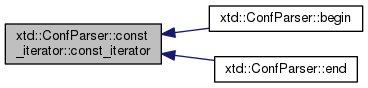
\includegraphics[width=348pt]{classxtd_1_1ConfParser_1_1const__iterator_a9c17a000740a8558dddb0dd1187939b5_icgraph}
\end{center}
\end{figure}


\index{xtd\+::\+Conf\+Parser\+::const\+\_\+iterator@{xtd\+::\+Conf\+Parser\+::const\+\_\+iterator}!const\+\_\+iterator@{const\+\_\+iterator}}
\index{const\+\_\+iterator@{const\+\_\+iterator}!xtd\+::\+Conf\+Parser\+::const\+\_\+iterator@{xtd\+::\+Conf\+Parser\+::const\+\_\+iterator}}
\subsubsection[{\texorpdfstring{const\+\_\+iterator(const const\+\_\+iterator \&p\+\_\+obj)}{const_iterator(const const_iterator &p_obj)}}]{\setlength{\rightskip}{0pt plus 5cm}xtd\+::\+Conf\+Parser\+::const\+\_\+iterator\+::const\+\_\+iterator (
\begin{DoxyParamCaption}
\item[{const {\bf const\+\_\+iterator} \&}]{p\+\_\+obj}
\end{DoxyParamCaption}
)\hspace{0.3cm}{\ttfamily [inline]}}\hypertarget{classxtd_1_1ConfParser_1_1const__iterator_af09c45149cd53e97902123aa770c0867}{}\label{classxtd_1_1ConfParser_1_1const__iterator_af09c45149cd53e97902123aa770c0867}


Definition at line 143 of file Conf\+Parser.\+hh.


\begin{DoxyCode}
144 \{
145   m\_iter = p\_obj.m\_iter;
146 \}
\end{DoxyCode}
\index{xtd\+::\+Conf\+Parser\+::const\+\_\+iterator@{xtd\+::\+Conf\+Parser\+::const\+\_\+iterator}!const\+\_\+iterator@{const\+\_\+iterator}}
\index{const\+\_\+iterator@{const\+\_\+iterator}!xtd\+::\+Conf\+Parser\+::const\+\_\+iterator@{xtd\+::\+Conf\+Parser\+::const\+\_\+iterator}}
\subsubsection[{\texorpdfstring{const\+\_\+iterator(const t\+\_\+section\+\_\+list\+::const\+\_\+iterator \&p\+\_\+iter)}{const_iterator(const t_section_list::const_iterator &p_iter)}}]{\setlength{\rightskip}{0pt plus 5cm}xtd\+::\+Conf\+Parser\+::const\+\_\+iterator\+::const\+\_\+iterator (
\begin{DoxyParamCaption}
\item[{const t\+\_\+section\+\_\+list\+::const\+\_\+iterator \&}]{p\+\_\+iter}
\end{DoxyParamCaption}
)\hspace{0.3cm}{\ttfamily [inline]}}\hypertarget{classxtd_1_1ConfParser_1_1const__iterator_a0fb34a1a672ceecfc5eb756e712bb977}{}\label{classxtd_1_1ConfParser_1_1const__iterator_a0fb34a1a672ceecfc5eb756e712bb977}


Definition at line 148 of file Conf\+Parser.\+hh.


\begin{DoxyCode}
149 \{
150   m\_iter = p\_iter;
151 \}
\end{DoxyCode}


\subsection{Member Function Documentation}
\index{xtd\+::\+Conf\+Parser\+::const\+\_\+iterator@{xtd\+::\+Conf\+Parser\+::const\+\_\+iterator}!operator"!=@{operator"!=}}
\index{operator"!=@{operator"!=}!xtd\+::\+Conf\+Parser\+::const\+\_\+iterator@{xtd\+::\+Conf\+Parser\+::const\+\_\+iterator}}
\subsubsection[{\texorpdfstring{operator"!=(const const\+\_\+iterator \&p\+\_\+obj) const }{operator!=(const const_iterator &p_obj) const }}]{\setlength{\rightskip}{0pt plus 5cm}bool xtd\+::\+Conf\+Parser\+::const\+\_\+iterator\+::operator!= (
\begin{DoxyParamCaption}
\item[{const {\bf const\+\_\+iterator} \&}]{p\+\_\+obj}
\end{DoxyParamCaption}
) const\hspace{0.3cm}{\ttfamily [inline]}}\hypertarget{classxtd_1_1ConfParser_1_1const__iterator_a380f55fdaee860e5cc7c4f8fcfade27b}{}\label{classxtd_1_1ConfParser_1_1const__iterator_a380f55fdaee860e5cc7c4f8fcfade27b}


Definition at line 188 of file Conf\+Parser.\+hh.


\begin{DoxyCode}
189 \{
190   \textcolor{keywordflow}{return} ! \hyperlink{classxtd_1_1ConfParser_1_1const__iterator_a1acb3ce9b1fb4892d77dcd649ec7768a}{operator==}(p\_obj);
191 \}
\end{DoxyCode}


Here is the call graph for this function\+:
\nopagebreak
\begin{figure}[H]
\begin{center}
\leavevmode
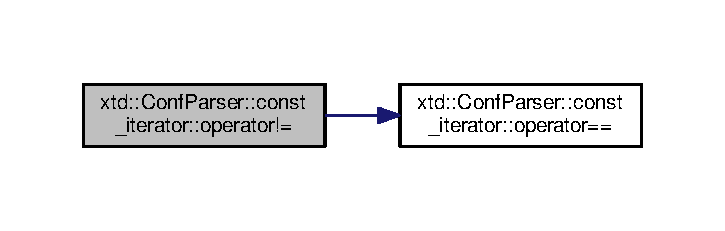
\includegraphics[width=348pt]{classxtd_1_1ConfParser_1_1const__iterator_a380f55fdaee860e5cc7c4f8fcfade27b_cgraph}
\end{center}
\end{figure}


\index{xtd\+::\+Conf\+Parser\+::const\+\_\+iterator@{xtd\+::\+Conf\+Parser\+::const\+\_\+iterator}!operator$\ast$@{operator$\ast$}}
\index{operator$\ast$@{operator$\ast$}!xtd\+::\+Conf\+Parser\+::const\+\_\+iterator@{xtd\+::\+Conf\+Parser\+::const\+\_\+iterator}}
\subsubsection[{\texorpdfstring{operator$\ast$(void) const }{operator*(void) const }}]{\setlength{\rightskip}{0pt plus 5cm}const Conf\+Parser\+::const\+\_\+iterator\+::t\+\_\+result xtd\+::\+Conf\+Parser\+::const\+\_\+iterator\+::operator$\ast$ (
\begin{DoxyParamCaption}
\item[{void}]{}
\end{DoxyParamCaption}
) const\hspace{0.3cm}{\ttfamily [inline]}}\hypertarget{classxtd_1_1ConfParser_1_1const__iterator_ab148b39b2f0e83242aeae432814eae7d}{}\label{classxtd_1_1ConfParser_1_1const__iterator_ab148b39b2f0e83242aeae432814eae7d}


Definition at line 174 of file Conf\+Parser.\+hh.


\begin{DoxyCode}
175 \{
176   \textcolor{keywordflow}{return} std::make\_pair(m\_iter->first.c\_str(),
177                         m\_iter->second.c\_str());
178 \}
\end{DoxyCode}
\index{xtd\+::\+Conf\+Parser\+::const\+\_\+iterator@{xtd\+::\+Conf\+Parser\+::const\+\_\+iterator}!operator++@{operator++}}
\index{operator++@{operator++}!xtd\+::\+Conf\+Parser\+::const\+\_\+iterator@{xtd\+::\+Conf\+Parser\+::const\+\_\+iterator}}
\subsubsection[{\texorpdfstring{operator++(void)}{operator++(void)}}]{\setlength{\rightskip}{0pt plus 5cm}void xtd\+::\+Conf\+Parser\+::const\+\_\+iterator\+::operator++ (
\begin{DoxyParamCaption}
\item[{void}]{}
\end{DoxyParamCaption}
)\hspace{0.3cm}{\ttfamily [inline]}}\hypertarget{classxtd_1_1ConfParser_1_1const__iterator_a6c3a5f37a31973077c3067a8d892aca0}{}\label{classxtd_1_1ConfParser_1_1const__iterator_a6c3a5f37a31973077c3067a8d892aca0}


Definition at line 168 of file Conf\+Parser.\+hh.


\begin{DoxyCode}
169 \{
170   ++m\_iter;
171 \}
\end{DoxyCode}
\index{xtd\+::\+Conf\+Parser\+::const\+\_\+iterator@{xtd\+::\+Conf\+Parser\+::const\+\_\+iterator}!operator++@{operator++}}
\index{operator++@{operator++}!xtd\+::\+Conf\+Parser\+::const\+\_\+iterator@{xtd\+::\+Conf\+Parser\+::const\+\_\+iterator}}
\subsubsection[{\texorpdfstring{operator++(int)}{operator++(int)}}]{\setlength{\rightskip}{0pt plus 5cm}void xtd\+::\+Conf\+Parser\+::const\+\_\+iterator\+::operator++ (
\begin{DoxyParamCaption}
\item[{int}]{}
\end{DoxyParamCaption}
)\hspace{0.3cm}{\ttfamily [inline]}}\hypertarget{classxtd_1_1ConfParser_1_1const__iterator_a7c5bfdfc6f85ac43469fc6dcd8601b98}{}\label{classxtd_1_1ConfParser_1_1const__iterator_a7c5bfdfc6f85ac43469fc6dcd8601b98}


Definition at line 162 of file Conf\+Parser.\+hh.


\begin{DoxyCode}
163 \{
164   m\_iter++;
165 \}
\end{DoxyCode}
\index{xtd\+::\+Conf\+Parser\+::const\+\_\+iterator@{xtd\+::\+Conf\+Parser\+::const\+\_\+iterator}!operator=@{operator=}}
\index{operator=@{operator=}!xtd\+::\+Conf\+Parser\+::const\+\_\+iterator@{xtd\+::\+Conf\+Parser\+::const\+\_\+iterator}}
\subsubsection[{\texorpdfstring{operator=(const const\+\_\+iterator \&p\+\_\+obj)}{operator=(const const_iterator &p_obj)}}]{\setlength{\rightskip}{0pt plus 5cm}{\bf Conf\+Parser\+::const\+\_\+iterator} \& xtd\+::\+Conf\+Parser\+::const\+\_\+iterator\+::operator= (
\begin{DoxyParamCaption}
\item[{const {\bf const\+\_\+iterator} \&}]{p\+\_\+obj}
\end{DoxyParamCaption}
)\hspace{0.3cm}{\ttfamily [inline]}}\hypertarget{classxtd_1_1ConfParser_1_1const__iterator_acef9a9b328552d35dec3b1736d775cf5}{}\label{classxtd_1_1ConfParser_1_1const__iterator_acef9a9b328552d35dec3b1736d775cf5}


Definition at line 154 of file Conf\+Parser.\+hh.


\begin{DoxyCode}
155 \{
156   m\_iter = p\_obj.m\_iter;
157   \textcolor{keywordflow}{return} *\textcolor{keyword}{this};
158 \}
\end{DoxyCode}
\index{xtd\+::\+Conf\+Parser\+::const\+\_\+iterator@{xtd\+::\+Conf\+Parser\+::const\+\_\+iterator}!operator==@{operator==}}
\index{operator==@{operator==}!xtd\+::\+Conf\+Parser\+::const\+\_\+iterator@{xtd\+::\+Conf\+Parser\+::const\+\_\+iterator}}
\subsubsection[{\texorpdfstring{operator==(const const\+\_\+iterator \&p\+\_\+obj) const }{operator==(const const_iterator &p_obj) const }}]{\setlength{\rightskip}{0pt plus 5cm}bool xtd\+::\+Conf\+Parser\+::const\+\_\+iterator\+::operator== (
\begin{DoxyParamCaption}
\item[{const {\bf const\+\_\+iterator} \&}]{p\+\_\+obj}
\end{DoxyParamCaption}
) const\hspace{0.3cm}{\ttfamily [inline]}}\hypertarget{classxtd_1_1ConfParser_1_1const__iterator_a1acb3ce9b1fb4892d77dcd649ec7768a}{}\label{classxtd_1_1ConfParser_1_1const__iterator_a1acb3ce9b1fb4892d77dcd649ec7768a}


Definition at line 182 of file Conf\+Parser.\+hh.


\begin{DoxyCode}
183 \{
184   \textcolor{keywordflow}{return} m\_iter == p\_obj.m\_iter;
185 \}
\end{DoxyCode}


Here is the caller graph for this function\+:
\nopagebreak
\begin{figure}[H]
\begin{center}
\leavevmode
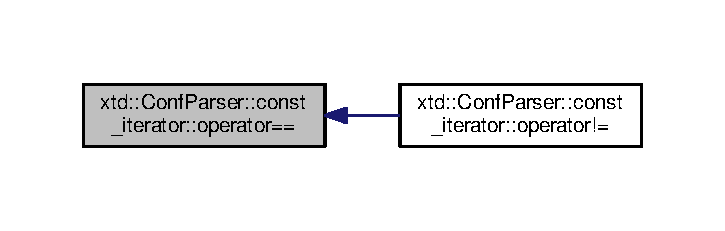
\includegraphics[width=348pt]{classxtd_1_1ConfParser_1_1const__iterator_a1acb3ce9b1fb4892d77dcd649ec7768a_icgraph}
\end{center}
\end{figure}




The documentation for this class was generated from the following file\+:\begin{DoxyCompactItemize}
\item 
/home/psyco/dev/xtdcpp/common/src/\hyperlink{ConfParser_8hh}{Conf\+Parser.\+hh}\end{DoxyCompactItemize}

\hypertarget{classxtd_1_1error}{\section{xtd\-:\-:error Class Reference}
\label{classxtd_1_1error}\index{xtd\-::error@{xtd\-::error}}
}


{\ttfamily \#include $<$error.\-hh$>$}



Inheritance diagram for xtd\-:\-:error\-:
\nopagebreak
\begin{figure}[H]
\begin{center}
\leavevmode
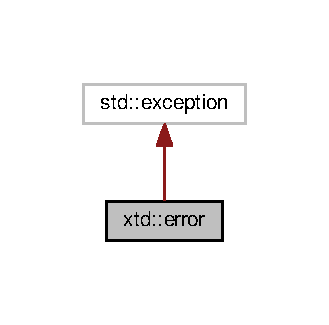
\includegraphics[width=158pt]{classxtd_1_1error__inherit__graph}
\end{center}
\end{figure}


Collaboration diagram for xtd\-:\-:error\-:
\nopagebreak
\begin{figure}[H]
\begin{center}
\leavevmode
\includegraphics[width=158pt]{classxtd_1_1error__coll__graph}
\end{center}
\end{figure}
\subsection*{Public Member Functions}
\begin{DoxyCompactItemize}
\item 
\hyperlink{classxtd_1_1error_a4663571e50d7bcf512b353660b897a55}{error} (const string \&p\-\_\-message)
\item 
virtual \hyperlink{classxtd_1_1error_abeceaf42dfbad136014dc3921696e26f}{$\sim$error} (void)
\item 
virtual const char $\ast$ \hyperlink{classxtd_1_1error_a463ff8177561abd418c1f00aa2bcd154}{what} () const   throw ()
\end{DoxyCompactItemize}
\subsection*{Static Public Member Functions}
\begin{DoxyCompactItemize}
\item 
{\footnotesize template$<$typename... Arguments$>$ }\\static void \hyperlink{classxtd_1_1error_a34fcbd60f169444fa6b9b410db6ddaaf}{do\-\_\-throw} (const string \&p\-\_\-module, const string \&p\-\_\-format, Arguments \&\&...p\-\_\-args)
\end{DoxyCompactItemize}


\subsection{Detailed Description}


Definition at line 8 of file error.\-hh.



\subsection{Constructor \& Destructor Documentation}
\hypertarget{classxtd_1_1error_a4663571e50d7bcf512b353660b897a55}{\index{xtd\-::error@{xtd\-::error}!error@{error}}
\index{error@{error}!xtd::error@{xtd\-::error}}
\subsubsection[{error}]{\setlength{\rightskip}{0pt plus 5cm}xtd\-::error\-::error (
\begin{DoxyParamCaption}
\item[{const string \&}]{p\-\_\-message}
\end{DoxyParamCaption}
)\hspace{0.3cm}{\ttfamily [inline]}}}\label{classxtd_1_1error_a4663571e50d7bcf512b353660b897a55}


Definition at line 19 of file error.\-hh.


\begin{DoxyCode}
19                                  :
20     m\_message(p\_message)
21   \{ \}
\end{DoxyCode}


Here is the caller graph for this function\-:
\nopagebreak
\begin{figure}[H]
\begin{center}
\leavevmode
\includegraphics[width=350pt]{classxtd_1_1error_a4663571e50d7bcf512b353660b897a55_icgraph}
\end{center}
\end{figure}


\hypertarget{classxtd_1_1error_abeceaf42dfbad136014dc3921696e26f}{\index{xtd\-::error@{xtd\-::error}!$\sim$error@{$\sim$error}}
\index{$\sim$error@{$\sim$error}!xtd::error@{xtd\-::error}}
\subsubsection[{$\sim$error}]{\setlength{\rightskip}{0pt plus 5cm}virtual xtd\-::error\-::$\sim$error (
\begin{DoxyParamCaption}
\item[{void}]{}
\end{DoxyParamCaption}
)\hspace{0.3cm}{\ttfamily [inline]}, {\ttfamily [virtual]}}}\label{classxtd_1_1error_abeceaf42dfbad136014dc3921696e26f}


Definition at line 22 of file error.\-hh.


\begin{DoxyCode}
23   \{ \}
\end{DoxyCode}


\subsection{Member Function Documentation}
\hypertarget{classxtd_1_1error_a34fcbd60f169444fa6b9b410db6ddaaf}{\index{xtd\-::error@{xtd\-::error}!do\-\_\-throw@{do\-\_\-throw}}
\index{do\-\_\-throw@{do\-\_\-throw}!xtd::error@{xtd\-::error}}
\subsubsection[{do\-\_\-throw}]{\setlength{\rightskip}{0pt plus 5cm}template$<$typename... Arguments$>$ static void xtd\-::error\-::do\-\_\-throw (
\begin{DoxyParamCaption}
\item[{const string \&}]{p\-\_\-module, }
\item[{const string \&}]{p\-\_\-format, }
\item[{Arguments \&\&...}]{p\-\_\-args}
\end{DoxyParamCaption}
)\hspace{0.3cm}{\ttfamily [inline]}, {\ttfamily [static]}}}\label{classxtd_1_1error_a34fcbd60f169444fa6b9b410db6ddaaf}


Definition at line 12 of file error.\-hh.


\begin{DoxyCode}
13   \{
14     \hyperlink{classxtd_1_1logger_a1725596996a6060db5055c499c9ec9d1}{logger::crit}(p\_module, p\_format, p\_args...);
15     \textcolor{keywordflow}{throw} \hyperlink{classxtd_1_1error_a4663571e50d7bcf512b353660b897a55}{error}(\hyperlink{classxtd_1_1logger_a169ce6459fe906cb5f840bdf2669e8ce}{logger::format\_vargs}(p\_format + \textcolor{stringliteral}{" in %s:%s:%d "}, p\_args...));
16   \}
\end{DoxyCode}


Here is the call graph for this function\-:
\nopagebreak
\begin{figure}[H]
\begin{center}
\leavevmode
\includegraphics[width=314pt]{classxtd_1_1error_a34fcbd60f169444fa6b9b410db6ddaaf_cgraph}
\end{center}
\end{figure}




Here is the caller graph for this function\-:
\nopagebreak
\begin{figure}[H]
\begin{center}
\leavevmode
\includegraphics[width=350pt]{classxtd_1_1error_a34fcbd60f169444fa6b9b410db6ddaaf_icgraph}
\end{center}
\end{figure}


\hypertarget{classxtd_1_1error_a463ff8177561abd418c1f00aa2bcd154}{\index{xtd\-::error@{xtd\-::error}!what@{what}}
\index{what@{what}!xtd::error@{xtd\-::error}}
\subsubsection[{what}]{\setlength{\rightskip}{0pt plus 5cm}virtual const char$\ast$ xtd\-::error\-::what (
\begin{DoxyParamCaption}
{}
\end{DoxyParamCaption}
) const throw  ) \hspace{0.3cm}{\ttfamily [inline]}, {\ttfamily [virtual]}}}\label{classxtd_1_1error_a463ff8177561abd418c1f00aa2bcd154}


Definition at line 26 of file error.\-hh.


\begin{DoxyCode}
27   \{
28     \textcolor{keywordflow}{return} m\_message.c\_str();
29   \}
\end{DoxyCode}


The documentation for this class was generated from the following file\-:\begin{DoxyCompactItemize}
\item 
/home/travis/build/psycofdj/xtdcpp/common/src/\hyperlink{error_8hh}{error.\-hh}\end{DoxyCompactItemize}

\hypertarget{classxtd_1_1logger}{}\section{xtd\+:\+:logger Class Reference}
\label{classxtd_1_1logger}\index{xtd\+::logger@{xtd\+::logger}}


{\ttfamily \#include $<$logger.\+hh$>$}

\subsection*{Public Types}
\begin{DoxyCompactItemize}
\item 
enum \hyperlink{classxtd_1_1logger_a250ce2f143da181d7149a1556da2a6f1}{level} \+: int32\+\_\+t \{ \\*
\hyperlink{classxtd_1_1logger_a250ce2f143da181d7149a1556da2a6f1ae6cb8d153a4c27be572a177366bd7abc}{level\+::emerg} = L\+O\+G\+\_\+\+E\+M\+E\+RG, 
\hyperlink{classxtd_1_1logger_a250ce2f143da181d7149a1556da2a6f1a7ed21143076d0cca420653d4345baa2f}{level\+::alert} = L\+O\+G\+\_\+\+A\+L\+E\+RT, 
\hyperlink{classxtd_1_1logger_a250ce2f143da181d7149a1556da2a6f1a5888c6a8bb862595985926d16c7dcf13}{level\+::crit} = L\+O\+G\+\_\+\+C\+R\+IT, 
\hyperlink{classxtd_1_1logger_a250ce2f143da181d7149a1556da2a6f1a56bd7107802ebe56c6918992f0608ec6}{level\+::err} = L\+O\+G\+\_\+\+E\+RR, 
\\*
\hyperlink{classxtd_1_1logger_a250ce2f143da181d7149a1556da2a6f1a7b83d3f08fa392b79e3f553b585971cd}{level\+::warning} = L\+O\+G\+\_\+\+W\+A\+R\+N\+I\+NG, 
\hyperlink{classxtd_1_1logger_a250ce2f143da181d7149a1556da2a6f1aefd2af60c8501931cb9c736b5ad74f65}{level\+::notice} = L\+O\+G\+\_\+\+N\+O\+T\+I\+CE, 
\hyperlink{classxtd_1_1logger_a250ce2f143da181d7149a1556da2a6f1acaf9b6b99962bf5c2264824231d7a40c}{level\+::info} = L\+O\+G\+\_\+\+I\+N\+FO, 
\hyperlink{classxtd_1_1logger_a250ce2f143da181d7149a1556da2a6f1aad42f6697b035b7580e4fef93be20b4d}{level\+::debug} = L\+O\+G\+\_\+\+D\+E\+B\+UG
 \}
\end{DoxyCompactItemize}
\subsection*{Public Member Functions}
\begin{DoxyCompactItemize}
\item 
\hyperlink{classxtd_1_1logger_a794da1cd7618a6796d639d11845f9006}{logger} (void)
\item 
void \hyperlink{classxtd_1_1logger_a586ddfe34d0f2c1343385f8034ef9b66}{initialize} (void)
\item 
void \hyperlink{classxtd_1_1logger_a8559c9744e68ecab37076d8744499c8f}{initialize} (const string \&p\+\_\+name, \hyperlink{classxtd_1_1logger_a250ce2f143da181d7149a1556da2a6f1}{level} p\+\_\+level)
\item 
void \hyperlink{classxtd_1_1logger_a9002910ed99cdc1df062c39e385cd379}{set\+Level} (const string \&p\+\_\+module, \hyperlink{classxtd_1_1logger_a250ce2f143da181d7149a1556da2a6f1}{level} p\+\_\+level)
\item 
void \hyperlink{classxtd_1_1logger_af88d4c20247cb62433e660ab7f9f5a97}{update\+Levels} (const string \&p\+\_\+regex, \hyperlink{classxtd_1_1logger_a250ce2f143da181d7149a1556da2a6f1}{level} p\+\_\+level)
\item 
void \hyperlink{classxtd_1_1logger_aeffebbe5b6a43f814c0a1251b6069f26}{set\+All\+Levels} (\hyperlink{classxtd_1_1logger_a250ce2f143da181d7149a1556da2a6f1}{level} p\+\_\+level)
\item 
void \hyperlink{classxtd_1_1logger_a10ec7455d964067fc1ca79f3a7cc14b4}{set\+All\+Value\+Levels} (uint32\+\_\+t p\+\_\+level)
\item 
void \hyperlink{classxtd_1_1logger_a18cd978561fcaf48e2fc935331834fe9}{clear\+All} (\hyperlink{classxtd_1_1logger_a250ce2f143da181d7149a1556da2a6f1}{level} p\+\_\+default)
\item 
void \hyperlink{classxtd_1_1logger_a314e15f9d6eeeafbcf93b2bb757e2143}{set\+Name} (const string \&p\+\_\+name)
\item 
\hyperlink{classxtd_1_1logger_a250ce2f143da181d7149a1556da2a6f1}{level} \hyperlink{classxtd_1_1logger_afa70268de8cc055f4903a54fa61c52df}{level\+Of} (const uint32\+\_\+t \&p\+\_\+level)
\item 
uint32\+\_\+t \hyperlink{classxtd_1_1logger_a615e10d21938ff8681a98894aa31490e}{value\+Of} (\hyperlink{classxtd_1_1logger_a250ce2f143da181d7149a1556da2a6f1}{level} p\+\_\+level)
\item 
string \hyperlink{classxtd_1_1logger_a791f6ccde4fa459cf05085d9b7a0f2d5}{string\+Of} (\hyperlink{classxtd_1_1logger_a250ce2f143da181d7149a1556da2a6f1}{level} p\+\_\+level)
\item 
\hyperlink{classxtd_1_1logger_a250ce2f143da181d7149a1556da2a6f1}{level} \hyperlink{classxtd_1_1logger_a88420216bbafe0a36bbd25080ac14567}{from\+String} (string p\+\_\+level)
\item 
\hyperlink{classxtd_1_1logger_a250ce2f143da181d7149a1556da2a6f1}{level} \hyperlink{classxtd_1_1logger_a4cb9dd27ead213c0a9f3d85d80e9a7b4}{get\+Level} (const string \&p\+\_\+module)
\item 
t\+\_\+levels \hyperlink{classxtd_1_1logger_a8b22d69269de5f4269fbbf43fe6f9b53}{get\+Levels} (void)
\item 
bool \hyperlink{classxtd_1_1logger_aaca2ec5d979b7f57c2060ecaac2715ec}{is\+Valid\+String\+Level} (string p\+\_\+level)
\end{DoxyCompactItemize}
\subsection*{Static Public Member Functions}
\begin{DoxyCompactItemize}
\item 
static \hyperlink{classxtd_1_1logger}{logger} \& \hyperlink{classxtd_1_1logger_a21511dfdad9ec1e88c3444637a000e9d}{get} (void)
\item 
{\footnotesize template$<$typename... Args$>$ }\\static void \hyperlink{classxtd_1_1logger_a07697b74619641014fb6e51130b5c837}{emerg} (const string \&p\+\_\+module, const string \&p\+\_\+format, Args...\+p\+\_\+args)
\item 
{\footnotesize template$<$typename... Args$>$ }\\static void \hyperlink{classxtd_1_1logger_abea0d6d16f6138d94e9373457fa08513}{alert} (const string \&p\+\_\+module, const string \&p\+\_\+format, Args...\+p\+\_\+args)
\item 
{\footnotesize template$<$typename... Args$>$ }\\static void \hyperlink{classxtd_1_1logger_a1725596996a6060db5055c499c9ec9d1}{crit} (const string \&p\+\_\+module, const string \&p\+\_\+format, Args...\+p\+\_\+args)
\item 
{\footnotesize template$<$typename... Args$>$ }\\static void \hyperlink{classxtd_1_1logger_a20f991c43e729cf84d5d5294b947091e}{err} (const string \&p\+\_\+module, const string \&p\+\_\+format, Args...\+p\+\_\+args)
\item 
{\footnotesize template$<$typename... Args$>$ }\\static void \hyperlink{classxtd_1_1logger_a7432d0a490aef6bfe2de6f5ff5b77c06}{warning} (const string \&p\+\_\+module, const string \&p\+\_\+format, Args...\+p\+\_\+args)
\item 
{\footnotesize template$<$typename... Args$>$ }\\static void \hyperlink{classxtd_1_1logger_ac6cf4c5d929c844041ea9763cc3926be}{info} (const string \&p\+\_\+module, const string \&p\+\_\+format, Args...\+p\+\_\+args)
\item 
{\footnotesize template$<$typename... Args$>$ }\\static void \hyperlink{classxtd_1_1logger_a74886bf7a5d2bb1f2b2bf0265b13b38b}{notice} (const string \&p\+\_\+module, const string \&p\+\_\+format, Args...\+p\+\_\+args)
\item 
{\footnotesize template$<$typename... Args$>$ }\\static void \hyperlink{classxtd_1_1logger_a53a77a287f7a29d9585898dcff910254}{debug} (const string \&p\+\_\+module, const string \&p\+\_\+format, Args...\+p\+\_\+args)
\item 
{\footnotesize template$<$typename... Arguments$>$ }\\static string \hyperlink{classxtd_1_1logger_a169ce6459fe906cb5f840bdf2669e8ce}{format\+\_\+vargs} (string const \&p\+\_\+fmt, Arguments \&\&...p\+\_\+args)
\end{DoxyCompactItemize}


\subsection{Detailed Description}


Definition at line 14 of file logger.\+hh.



\subsection{Member Enumeration Documentation}
\index{xtd\+::logger@{xtd\+::logger}!level@{level}}
\index{level@{level}!xtd\+::logger@{xtd\+::logger}}
\subsubsection[{\texorpdfstring{level}{level}}]{\setlength{\rightskip}{0pt plus 5cm}enum {\bf xtd\+::logger\+::level} \+: int32\+\_\+t\hspace{0.3cm}{\ttfamily [strong]}}\hypertarget{classxtd_1_1logger_a250ce2f143da181d7149a1556da2a6f1}{}\label{classxtd_1_1logger_a250ce2f143da181d7149a1556da2a6f1}
\begin{Desc}
\item[Enumerator]\par
\begin{description}
\index{emerg@{emerg}!xtd\+::logger@{xtd\+::logger}}\index{xtd\+::logger@{xtd\+::logger}!emerg@{emerg}}\item[{\em 
emerg\hypertarget{classxtd_1_1logger_a250ce2f143da181d7149a1556da2a6f1ae6cb8d153a4c27be572a177366bd7abc}{}\label{classxtd_1_1logger_a250ce2f143da181d7149a1556da2a6f1ae6cb8d153a4c27be572a177366bd7abc}
}]\index{alert@{alert}!xtd\+::logger@{xtd\+::logger}}\index{xtd\+::logger@{xtd\+::logger}!alert@{alert}}\item[{\em 
alert\hypertarget{classxtd_1_1logger_a250ce2f143da181d7149a1556da2a6f1a7ed21143076d0cca420653d4345baa2f}{}\label{classxtd_1_1logger_a250ce2f143da181d7149a1556da2a6f1a7ed21143076d0cca420653d4345baa2f}
}]\index{crit@{crit}!xtd\+::logger@{xtd\+::logger}}\index{xtd\+::logger@{xtd\+::logger}!crit@{crit}}\item[{\em 
crit\hypertarget{classxtd_1_1logger_a250ce2f143da181d7149a1556da2a6f1a5888c6a8bb862595985926d16c7dcf13}{}\label{classxtd_1_1logger_a250ce2f143da181d7149a1556da2a6f1a5888c6a8bb862595985926d16c7dcf13}
}]\index{err@{err}!xtd\+::logger@{xtd\+::logger}}\index{xtd\+::logger@{xtd\+::logger}!err@{err}}\item[{\em 
err\hypertarget{classxtd_1_1logger_a250ce2f143da181d7149a1556da2a6f1a56bd7107802ebe56c6918992f0608ec6}{}\label{classxtd_1_1logger_a250ce2f143da181d7149a1556da2a6f1a56bd7107802ebe56c6918992f0608ec6}
}]\index{warning@{warning}!xtd\+::logger@{xtd\+::logger}}\index{xtd\+::logger@{xtd\+::logger}!warning@{warning}}\item[{\em 
warning\hypertarget{classxtd_1_1logger_a250ce2f143da181d7149a1556da2a6f1a7b83d3f08fa392b79e3f553b585971cd}{}\label{classxtd_1_1logger_a250ce2f143da181d7149a1556da2a6f1a7b83d3f08fa392b79e3f553b585971cd}
}]\index{notice@{notice}!xtd\+::logger@{xtd\+::logger}}\index{xtd\+::logger@{xtd\+::logger}!notice@{notice}}\item[{\em 
notice\hypertarget{classxtd_1_1logger_a250ce2f143da181d7149a1556da2a6f1aefd2af60c8501931cb9c736b5ad74f65}{}\label{classxtd_1_1logger_a250ce2f143da181d7149a1556da2a6f1aefd2af60c8501931cb9c736b5ad74f65}
}]\index{info@{info}!xtd\+::logger@{xtd\+::logger}}\index{xtd\+::logger@{xtd\+::logger}!info@{info}}\item[{\em 
info\hypertarget{classxtd_1_1logger_a250ce2f143da181d7149a1556da2a6f1acaf9b6b99962bf5c2264824231d7a40c}{}\label{classxtd_1_1logger_a250ce2f143da181d7149a1556da2a6f1acaf9b6b99962bf5c2264824231d7a40c}
}]\index{debug@{debug}!xtd\+::logger@{xtd\+::logger}}\index{xtd\+::logger@{xtd\+::logger}!debug@{debug}}\item[{\em 
debug\hypertarget{classxtd_1_1logger_a250ce2f143da181d7149a1556da2a6f1aad42f6697b035b7580e4fef93be20b4d}{}\label{classxtd_1_1logger_a250ce2f143da181d7149a1556da2a6f1aad42f6697b035b7580e4fef93be20b4d}
}]\end{description}
\end{Desc}


Definition at line 17 of file logger.\+hh.


\begin{DoxyCode}
17                    : int32\_t \{
18     \hyperlink{classxtd_1_1logger_a07697b74619641014fb6e51130b5c837}{emerg}   = LOG\_EMERG,
19       \hyperlink{classxtd_1_1logger_abea0d6d16f6138d94e9373457fa08513}{alert}   = LOG\_ALERT,
20       \hyperlink{classxtd_1_1logger_a1725596996a6060db5055c499c9ec9d1}{crit}    = LOG\_CRIT,
21       \hyperlink{classxtd_1_1logger_a20f991c43e729cf84d5d5294b947091e}{err}     = LOG\_ERR,
22       \hyperlink{classxtd_1_1logger_a7432d0a490aef6bfe2de6f5ff5b77c06}{warning} = LOG\_WARNING,
23       \hyperlink{classxtd_1_1logger_a74886bf7a5d2bb1f2b2bf0265b13b38b}{notice}  = LOG\_NOTICE,
24       \hyperlink{classxtd_1_1logger_ac6cf4c5d929c844041ea9763cc3926be}{info}    = LOG\_INFO,
25       \hyperlink{classxtd_1_1logger_a53a77a287f7a29d9585898dcff910254}{debug}   = LOG\_DEBUG
26       \};
\end{DoxyCode}


\subsection{Constructor \& Destructor Documentation}
\index{xtd\+::logger@{xtd\+::logger}!logger@{logger}}
\index{logger@{logger}!xtd\+::logger@{xtd\+::logger}}
\subsubsection[{\texorpdfstring{logger(void)}{logger(void)}}]{\setlength{\rightskip}{0pt plus 5cm}xtd\+::logger\+::logger (
\begin{DoxyParamCaption}
\item[{void}]{}
\end{DoxyParamCaption}
)}\hypertarget{classxtd_1_1logger_a794da1cd7618a6796d639d11845f9006}{}\label{classxtd_1_1logger_a794da1cd7618a6796d639d11845f9006}


Definition at line 11 of file logger.\+cc.


\begin{DoxyCode}
11                    :
12   m\_name(\textcolor{stringliteral}{"unknown"})
13 \{
14 \}
\end{DoxyCode}


Here is the caller graph for this function\+:
\nopagebreak
\begin{figure}[H]
\begin{center}
\leavevmode
\includegraphics[width=350pt]{classxtd_1_1logger_a794da1cd7618a6796d639d11845f9006_icgraph}
\end{center}
\end{figure}




\subsection{Member Function Documentation}
\index{xtd\+::logger@{xtd\+::logger}!alert@{alert}}
\index{alert@{alert}!xtd\+::logger@{xtd\+::logger}}
\subsubsection[{\texorpdfstring{alert(const string \&p\+\_\+module, const string \&p\+\_\+format, Args...\+p\+\_\+args)}{alert(const string &p_module, const string &p_format, Args...p_args)}}]{\setlength{\rightskip}{0pt plus 5cm}template$<$typename... Args$>$ static void xtd\+::logger\+::alert (
\begin{DoxyParamCaption}
\item[{const string \&}]{p\+\_\+module, }
\item[{const string \&}]{p\+\_\+format, }
\item[{Args...}]{p\+\_\+args}
\end{DoxyParamCaption}
)\hspace{0.3cm}{\ttfamily [static]}}\hypertarget{classxtd_1_1logger_abea0d6d16f6138d94e9373457fa08513}{}\label{classxtd_1_1logger_abea0d6d16f6138d94e9373457fa08513}
\index{xtd\+::logger@{xtd\+::logger}!clear\+All@{clear\+All}}
\index{clear\+All@{clear\+All}!xtd\+::logger@{xtd\+::logger}}
\subsubsection[{\texorpdfstring{clear\+All(level p\+\_\+default)}{clearAll(level p_default)}}]{\setlength{\rightskip}{0pt plus 5cm}void xtd\+::logger\+::clear\+All (
\begin{DoxyParamCaption}
\item[{{\bf level}}]{p\+\_\+default}
\end{DoxyParamCaption}
)}\hypertarget{classxtd_1_1logger_a18cd978561fcaf48e2fc935331834fe9}{}\label{classxtd_1_1logger_a18cd978561fcaf48e2fc935331834fe9}


Definition at line 55 of file logger.\+cc.


\begin{DoxyCode}
56 \{
57   m\_levels.clear();
58   \hyperlink{classxtd_1_1logger_a9002910ed99cdc1df062c39e385cd379}{setLevel}(\textcolor{stringliteral}{""}, p\_level);
59 \}
\end{DoxyCode}


Here is the call graph for this function\+:
\nopagebreak
\begin{figure}[H]
\begin{center}
\leavevmode
\includegraphics[width=322pt]{classxtd_1_1logger_a18cd978561fcaf48e2fc935331834fe9_cgraph}
\end{center}
\end{figure}


\index{xtd\+::logger@{xtd\+::logger}!crit@{crit}}
\index{crit@{crit}!xtd\+::logger@{xtd\+::logger}}
\subsubsection[{\texorpdfstring{crit(const string \&p\+\_\+module, const string \&p\+\_\+format, Args...\+p\+\_\+args)}{crit(const string &p_module, const string &p_format, Args...p_args)}}]{\setlength{\rightskip}{0pt plus 5cm}template$<$typename... Args$>$ static void xtd\+::logger\+::crit (
\begin{DoxyParamCaption}
\item[{const string \&}]{p\+\_\+module, }
\item[{const string \&}]{p\+\_\+format, }
\item[{Args...}]{p\+\_\+args}
\end{DoxyParamCaption}
)\hspace{0.3cm}{\ttfamily [static]}}\hypertarget{classxtd_1_1logger_a1725596996a6060db5055c499c9ec9d1}{}\label{classxtd_1_1logger_a1725596996a6060db5055c499c9ec9d1}


Here is the caller graph for this function\+:
\nopagebreak
\begin{figure}[H]
\begin{center}
\leavevmode
\includegraphics[width=350pt]{classxtd_1_1logger_a1725596996a6060db5055c499c9ec9d1_icgraph}
\end{center}
\end{figure}


\index{xtd\+::logger@{xtd\+::logger}!debug@{debug}}
\index{debug@{debug}!xtd\+::logger@{xtd\+::logger}}
\subsubsection[{\texorpdfstring{debug(const string \&p\+\_\+module, const string \&p\+\_\+format, Args...\+p\+\_\+args)}{debug(const string &p_module, const string &p_format, Args...p_args)}}]{\setlength{\rightskip}{0pt plus 5cm}template$<$typename... Args$>$ static void xtd\+::logger\+::debug (
\begin{DoxyParamCaption}
\item[{const string \&}]{p\+\_\+module, }
\item[{const string \&}]{p\+\_\+format, }
\item[{Args...}]{p\+\_\+args}
\end{DoxyParamCaption}
)\hspace{0.3cm}{\ttfamily [static]}}\hypertarget{classxtd_1_1logger_a53a77a287f7a29d9585898dcff910254}{}\label{classxtd_1_1logger_a53a77a287f7a29d9585898dcff910254}


Here is the caller graph for this function\+:
\nopagebreak
\begin{figure}[H]
\begin{center}
\leavevmode
\includegraphics[width=350pt]{classxtd_1_1logger_a53a77a287f7a29d9585898dcff910254_icgraph}
\end{center}
\end{figure}


\index{xtd\+::logger@{xtd\+::logger}!emerg@{emerg}}
\index{emerg@{emerg}!xtd\+::logger@{xtd\+::logger}}
\subsubsection[{\texorpdfstring{emerg(const string \&p\+\_\+module, const string \&p\+\_\+format, Args...\+p\+\_\+args)}{emerg(const string &p_module, const string &p_format, Args...p_args)}}]{\setlength{\rightskip}{0pt plus 5cm}template$<$typename... Args$>$ static void xtd\+::logger\+::emerg (
\begin{DoxyParamCaption}
\item[{const string \&}]{p\+\_\+module, }
\item[{const string \&}]{p\+\_\+format, }
\item[{Args...}]{p\+\_\+args}
\end{DoxyParamCaption}
)\hspace{0.3cm}{\ttfamily [static]}}\hypertarget{classxtd_1_1logger_a07697b74619641014fb6e51130b5c837}{}\label{classxtd_1_1logger_a07697b74619641014fb6e51130b5c837}
\index{xtd\+::logger@{xtd\+::logger}!err@{err}}
\index{err@{err}!xtd\+::logger@{xtd\+::logger}}
\subsubsection[{\texorpdfstring{err(const string \&p\+\_\+module, const string \&p\+\_\+format, Args...\+p\+\_\+args)}{err(const string &p_module, const string &p_format, Args...p_args)}}]{\setlength{\rightskip}{0pt plus 5cm}template$<$typename... Args$>$ static void xtd\+::logger\+::err (
\begin{DoxyParamCaption}
\item[{const string \&}]{p\+\_\+module, }
\item[{const string \&}]{p\+\_\+format, }
\item[{Args...}]{p\+\_\+args}
\end{DoxyParamCaption}
)\hspace{0.3cm}{\ttfamily [static]}}\hypertarget{classxtd_1_1logger_a20f991c43e729cf84d5d5294b947091e}{}\label{classxtd_1_1logger_a20f991c43e729cf84d5d5294b947091e}


Here is the caller graph for this function\+:
\nopagebreak
\begin{figure}[H]
\begin{center}
\leavevmode
\includegraphics[width=337pt]{classxtd_1_1logger_a20f991c43e729cf84d5d5294b947091e_icgraph}
\end{center}
\end{figure}


\index{xtd\+::logger@{xtd\+::logger}!format\+\_\+vargs@{format\+\_\+vargs}}
\index{format\+\_\+vargs@{format\+\_\+vargs}!xtd\+::logger@{xtd\+::logger}}
\subsubsection[{\texorpdfstring{format\+\_\+vargs(string const \&p\+\_\+fmt, Arguments \&\&...\+p\+\_\+args)}{format_vargs(string const &p_fmt, Arguments &&...p_args)}}]{\setlength{\rightskip}{0pt plus 5cm}template$<$typename... Arguments$>$ static string xtd\+::logger\+::format\+\_\+vargs (
\begin{DoxyParamCaption}
\item[{string const \&}]{p\+\_\+fmt, }
\item[{Arguments \&\&...}]{p\+\_\+args}
\end{DoxyParamCaption}
)\hspace{0.3cm}{\ttfamily [static]}}\hypertarget{classxtd_1_1logger_a169ce6459fe906cb5f840bdf2669e8ce}{}\label{classxtd_1_1logger_a169ce6459fe906cb5f840bdf2669e8ce}


Here is the caller graph for this function\+:
\nopagebreak
\begin{figure}[H]
\begin{center}
\leavevmode
\includegraphics[width=350pt]{classxtd_1_1logger_a169ce6459fe906cb5f840bdf2669e8ce_icgraph}
\end{center}
\end{figure}


\index{xtd\+::logger@{xtd\+::logger}!from\+String@{from\+String}}
\index{from\+String@{from\+String}!xtd\+::logger@{xtd\+::logger}}
\subsubsection[{\texorpdfstring{from\+String(string p\+\_\+level)}{fromString(string p_level)}}]{\setlength{\rightskip}{0pt plus 5cm}{\bf logger\+::level} xtd\+::logger\+::from\+String (
\begin{DoxyParamCaption}
\item[{string}]{p\+\_\+level}
\end{DoxyParamCaption}
)}\hypertarget{classxtd_1_1logger_a88420216bbafe0a36bbd25080ac14567}{}\label{classxtd_1_1logger_a88420216bbafe0a36bbd25080ac14567}


Definition at line 222 of file logger.\+cc.


\begin{DoxyCode}
223 \{
224   \textcolor{keywordflow}{if} (p\_level == \textcolor{stringliteral}{"emerg"})
225     \textcolor{keywordflow}{return} \hyperlink{classxtd_1_1logger_a250ce2f143da181d7149a1556da2a6f1ae6cb8d153a4c27be572a177366bd7abc}{level::emerg};
226   \textcolor{keywordflow}{if} (p\_level == \textcolor{stringliteral}{"alert"})
227     \textcolor{keywordflow}{return} \hyperlink{classxtd_1_1logger_a250ce2f143da181d7149a1556da2a6f1a7ed21143076d0cca420653d4345baa2f}{level::alert};
228   \textcolor{keywordflow}{if} (p\_level == \textcolor{stringliteral}{"crit"})
229     \textcolor{keywordflow}{return} \hyperlink{classxtd_1_1logger_a250ce2f143da181d7149a1556da2a6f1a5888c6a8bb862595985926d16c7dcf13}{level::crit};
230   \textcolor{keywordflow}{if} (p\_level == \textcolor{stringliteral}{"err"})
231     \textcolor{keywordflow}{return} \hyperlink{classxtd_1_1logger_a250ce2f143da181d7149a1556da2a6f1a56bd7107802ebe56c6918992f0608ec6}{level::err};
232   \textcolor{keywordflow}{if} (p\_level == \textcolor{stringliteral}{"warning"})
233     \textcolor{keywordflow}{return} \hyperlink{classxtd_1_1logger_a250ce2f143da181d7149a1556da2a6f1a7b83d3f08fa392b79e3f553b585971cd}{level::warning};
234   \textcolor{keywordflow}{if} (p\_level == \textcolor{stringliteral}{"notice"})
235     \textcolor{keywordflow}{return} \hyperlink{classxtd_1_1logger_a250ce2f143da181d7149a1556da2a6f1aefd2af60c8501931cb9c736b5ad74f65}{level::notice};
236   \textcolor{keywordflow}{if} (p\_level == \textcolor{stringliteral}{"info"})
237     \textcolor{keywordflow}{return} \hyperlink{classxtd_1_1logger_a250ce2f143da181d7149a1556da2a6f1acaf9b6b99962bf5c2264824231d7a40c}{level::info};
238   \textcolor{keywordflow}{if} (p\_level == \textcolor{stringliteral}{"debug"})
239     \textcolor{keywordflow}{return} \hyperlink{classxtd_1_1logger_a250ce2f143da181d7149a1556da2a6f1aad42f6697b035b7580e4fef93be20b4d}{level::debug};
240   \textcolor{keywordflow}{return} \hyperlink{classxtd_1_1logger_a250ce2f143da181d7149a1556da2a6f1a5888c6a8bb862595985926d16c7dcf13}{level::crit};
241 \}
\end{DoxyCode}
\index{xtd\+::logger@{xtd\+::logger}!get@{get}}
\index{get@{get}!xtd\+::logger@{xtd\+::logger}}
\subsubsection[{\texorpdfstring{get(void)}{get(void)}}]{\setlength{\rightskip}{0pt plus 5cm}{\bf logger} \& xtd\+::logger\+::get (
\begin{DoxyParamCaption}
\item[{void}]{}
\end{DoxyParamCaption}
)\hspace{0.3cm}{\ttfamily [static]}}\hypertarget{classxtd_1_1logger_a21511dfdad9ec1e88c3444637a000e9d}{}\label{classxtd_1_1logger_a21511dfdad9ec1e88c3444637a000e9d}


Definition at line 17 of file logger.\+cc.


\begin{DoxyCode}
18 \{
19   \textcolor{keywordflow}{if} (0 == ms\_pInstance)
20     ms\_pInstance = \textcolor{keyword}{new} \hyperlink{classxtd_1_1logger_a794da1cd7618a6796d639d11845f9006}{logger}();
21   \textcolor{keywordflow}{return} *ms\_pInstance;
22 \}
\end{DoxyCode}


Here is the call graph for this function\+:
\nopagebreak
\begin{figure}[H]
\begin{center}
\leavevmode
\includegraphics[width=293pt]{classxtd_1_1logger_a21511dfdad9ec1e88c3444637a000e9d_cgraph}
\end{center}
\end{figure}




Here is the caller graph for this function\+:
\nopagebreak
\begin{figure}[H]
\begin{center}
\leavevmode
\includegraphics[width=350pt]{classxtd_1_1logger_a21511dfdad9ec1e88c3444637a000e9d_icgraph}
\end{center}
\end{figure}


\index{xtd\+::logger@{xtd\+::logger}!get\+Level@{get\+Level}}
\index{get\+Level@{get\+Level}!xtd\+::logger@{xtd\+::logger}}
\subsubsection[{\texorpdfstring{get\+Level(const string \&p\+\_\+module)}{getLevel(const string &p_module)}}]{\setlength{\rightskip}{0pt plus 5cm}{\bf logger\+::level} xtd\+::logger\+::get\+Level (
\begin{DoxyParamCaption}
\item[{const string \&}]{p\+\_\+module}
\end{DoxyParamCaption}
)}\hypertarget{classxtd_1_1logger_a4cb9dd27ead213c0a9f3d85d80e9a7b4}{}\label{classxtd_1_1logger_a4cb9dd27ead213c0a9f3d85d80e9a7b4}


Definition at line 103 of file logger.\+cc.


\begin{DoxyCode}
104 \{
105   \textcolor{keyword}{auto}                     c\_res = m\_levels.find(p\_module);
106   \hyperlink{classxtd_1_1logger_a250ce2f143da181d7149a1556da2a6f1}{level}                    l\_result = \hyperlink{classxtd_1_1logger_a250ce2f143da181d7149a1556da2a6f1a5888c6a8bb862595985926d16c7dcf13}{level::crit};
107   vector<string>           l\_parts;
108   vector<string>::iterator c\_part;
109 
110   \textcolor{keywordflow}{if} (c\_res != m\_levels.end())
111     \textcolor{keywordflow}{return} c\_res->second;
112 
113   boost::split(l\_parts, p\_module, boost::is\_any\_of(\textcolor{stringliteral}{"."}), boost::token\_compress\_on);
114   c\_part = l\_parts.end();
115 
116   \textcolor{keywordflow}{while} (c\_res == m\_levels.end())
117   \{
118     c\_part--;
119     vector<string> l\_tmp(l\_parts.begin(), c\_part);
120     c\_res = m\_levels.find(boost::join(l\_tmp, \textcolor{stringliteral}{"."}));
121   \}
122 
123   \textcolor{keywordflow}{if} (c\_res != m\_levels.end())
124     l\_result = c\_res->second;
125 
126   \hyperlink{classxtd_1_1logger_a9002910ed99cdc1df062c39e385cd379}{setLevel}(p\_module, l\_result);
127   \textcolor{keywordflow}{return} \hyperlink{classxtd_1_1logger_a250ce2f143da181d7149a1556da2a6f1a5888c6a8bb862595985926d16c7dcf13}{level::crit};
128 \}
\end{DoxyCode}


Here is the call graph for this function\+:
\nopagebreak
\begin{figure}[H]
\begin{center}
\leavevmode
\includegraphics[width=326pt]{classxtd_1_1logger_a4cb9dd27ead213c0a9f3d85d80e9a7b4_cgraph}
\end{center}
\end{figure}


\index{xtd\+::logger@{xtd\+::logger}!get\+Levels@{get\+Levels}}
\index{get\+Levels@{get\+Levels}!xtd\+::logger@{xtd\+::logger}}
\subsubsection[{\texorpdfstring{get\+Levels(void)}{getLevels(void)}}]{\setlength{\rightskip}{0pt plus 5cm}logger\+::t\+\_\+levels xtd\+::logger\+::get\+Levels (
\begin{DoxyParamCaption}
\item[{void}]{}
\end{DoxyParamCaption}
)}\hypertarget{classxtd_1_1logger_a8b22d69269de5f4269fbbf43fe6f9b53}{}\label{classxtd_1_1logger_a8b22d69269de5f4269fbbf43fe6f9b53}


Definition at line 75 of file logger.\+cc.


\begin{DoxyCode}
76 \{
77   \textcolor{keywordflow}{return} m\_levels;
78 \}
\end{DoxyCode}
\index{xtd\+::logger@{xtd\+::logger}!info@{info}}
\index{info@{info}!xtd\+::logger@{xtd\+::logger}}
\subsubsection[{\texorpdfstring{info(const string \&p\+\_\+module, const string \&p\+\_\+format, Args...\+p\+\_\+args)}{info(const string &p_module, const string &p_format, Args...p_args)}}]{\setlength{\rightskip}{0pt plus 5cm}template$<$typename... Args$>$ static void xtd\+::logger\+::info (
\begin{DoxyParamCaption}
\item[{const string \&}]{p\+\_\+module, }
\item[{const string \&}]{p\+\_\+format, }
\item[{Args...}]{p\+\_\+args}
\end{DoxyParamCaption}
)\hspace{0.3cm}{\ttfamily [static]}}\hypertarget{classxtd_1_1logger_ac6cf4c5d929c844041ea9763cc3926be}{}\label{classxtd_1_1logger_ac6cf4c5d929c844041ea9763cc3926be}


Here is the caller graph for this function\+:
\nopagebreak
\begin{figure}[H]
\begin{center}
\leavevmode
\includegraphics[width=305pt]{classxtd_1_1logger_ac6cf4c5d929c844041ea9763cc3926be_icgraph}
\end{center}
\end{figure}


\index{xtd\+::logger@{xtd\+::logger}!initialize@{initialize}}
\index{initialize@{initialize}!xtd\+::logger@{xtd\+::logger}}
\subsubsection[{\texorpdfstring{initialize(void)}{initialize(void)}}]{\setlength{\rightskip}{0pt plus 5cm}void xtd\+::logger\+::initialize (
\begin{DoxyParamCaption}
\item[{void}]{}
\end{DoxyParamCaption}
)}\hypertarget{classxtd_1_1logger_a586ddfe34d0f2c1343385f8034ef9b66}{}\label{classxtd_1_1logger_a586ddfe34d0f2c1343385f8034ef9b66}


Definition at line 34 of file logger.\+cc.


\begin{DoxyCode}
35 \{
36   \hyperlink{classxtd_1_1logger_a586ddfe34d0f2c1343385f8034ef9b66}{initialize}(m\_name, \hyperlink{classxtd_1_1logger_a250ce2f143da181d7149a1556da2a6f1a5888c6a8bb862595985926d16c7dcf13}{level::crit});
37 \}
\end{DoxyCode}


Here is the caller graph for this function\+:
\nopagebreak
\begin{figure}[H]
\begin{center}
\leavevmode
\includegraphics[width=350pt]{classxtd_1_1logger_a586ddfe34d0f2c1343385f8034ef9b66_icgraph}
\end{center}
\end{figure}


\index{xtd\+::logger@{xtd\+::logger}!initialize@{initialize}}
\index{initialize@{initialize}!xtd\+::logger@{xtd\+::logger}}
\subsubsection[{\texorpdfstring{initialize(const string \&p\+\_\+name, level p\+\_\+level)}{initialize(const string &p_name, level p_level)}}]{\setlength{\rightskip}{0pt plus 5cm}void xtd\+::logger\+::initialize (
\begin{DoxyParamCaption}
\item[{const string \&}]{p\+\_\+name, }
\item[{{\bf level}}]{p\+\_\+level}
\end{DoxyParamCaption}
)}\hypertarget{classxtd_1_1logger_a8559c9744e68ecab37076d8744499c8f}{}\label{classxtd_1_1logger_a8559c9744e68ecab37076d8744499c8f}


Definition at line 40 of file logger.\+cc.


\begin{DoxyCode}
41 \{
42   \hyperlink{classxtd_1_1logger_a314e15f9d6eeeafbcf93b2bb757e2143}{setName}(p\_name);
43   \hyperlink{classxtd_1_1logger_a9002910ed99cdc1df062c39e385cd379}{setLevel}(\textcolor{stringliteral}{""}, p\_level);
44   openlog(m\_name.c\_str(), LOG\_PID | LOG\_PERROR, LOG\_LOCAL0);
45   m\_initialized = \textcolor{keyword}{true};
46 \}
\end{DoxyCode}


Here is the call graph for this function\+:
\nopagebreak
\begin{figure}[H]
\begin{center}
\leavevmode
\includegraphics[width=328pt]{classxtd_1_1logger_a8559c9744e68ecab37076d8744499c8f_cgraph}
\end{center}
\end{figure}


\index{xtd\+::logger@{xtd\+::logger}!is\+Valid\+String\+Level@{is\+Valid\+String\+Level}}
\index{is\+Valid\+String\+Level@{is\+Valid\+String\+Level}!xtd\+::logger@{xtd\+::logger}}
\subsubsection[{\texorpdfstring{is\+Valid\+String\+Level(string p\+\_\+level)}{isValidStringLevel(string p_level)}}]{\setlength{\rightskip}{0pt plus 5cm}bool xtd\+::logger\+::is\+Valid\+String\+Level (
\begin{DoxyParamCaption}
\item[{string}]{p\+\_\+level}
\end{DoxyParamCaption}
)}\hypertarget{classxtd_1_1logger_aaca2ec5d979b7f57c2060ecaac2715ec}{}\label{classxtd_1_1logger_aaca2ec5d979b7f57c2060ecaac2715ec}


Definition at line 181 of file logger.\+cc.


\begin{DoxyCode}
182 \{
183   \textcolor{keywordflow}{return}
184     ((p\_level == \textcolor{stringliteral}{"emerg"})   ||
185      (p\_level == \textcolor{stringliteral}{"alert"})   ||
186      (p\_level == \textcolor{stringliteral}{"crit"})    ||
187      (p\_level == \textcolor{stringliteral}{"err"})     ||
188      (p\_level == \textcolor{stringliteral}{"warning"}) ||
189      (p\_level == \textcolor{stringliteral}{"notice"})  ||
190      (p\_level == \textcolor{stringliteral}{"info"})    ||
191      (p\_level == \textcolor{stringliteral}{"debug"}));
192 \}
\end{DoxyCode}
\index{xtd\+::logger@{xtd\+::logger}!level\+Of@{level\+Of}}
\index{level\+Of@{level\+Of}!xtd\+::logger@{xtd\+::logger}}
\subsubsection[{\texorpdfstring{level\+Of(const uint32\+\_\+t \&p\+\_\+level)}{levelOf(const uint32_t &p_level)}}]{\setlength{\rightskip}{0pt plus 5cm}{\bf logger\+::level} xtd\+::logger\+::level\+Of (
\begin{DoxyParamCaption}
\item[{const uint32\+\_\+t \&}]{p\+\_\+level}
\end{DoxyParamCaption}
)}\hypertarget{classxtd_1_1logger_afa70268de8cc055f4903a54fa61c52df}{}\label{classxtd_1_1logger_afa70268de8cc055f4903a54fa61c52df}


Definition at line 133 of file logger.\+cc.


\begin{DoxyCode}
134 \{
135   \textcolor{keywordflow}{if} (p\_level == LOG\_EMERG)
136     \textcolor{keywordflow}{return} \hyperlink{classxtd_1_1logger_a250ce2f143da181d7149a1556da2a6f1ae6cb8d153a4c27be572a177366bd7abc}{level::emerg};
137   \textcolor{keywordflow}{else} \textcolor{keywordflow}{if} (p\_level == LOG\_ALERT)
138     \textcolor{keywordflow}{return} \hyperlink{classxtd_1_1logger_a250ce2f143da181d7149a1556da2a6f1a7ed21143076d0cca420653d4345baa2f}{level::alert};
139   \textcolor{keywordflow}{else} \textcolor{keywordflow}{if} (p\_level == LOG\_CRIT)
140     \textcolor{keywordflow}{return} \hyperlink{classxtd_1_1logger_a250ce2f143da181d7149a1556da2a6f1a5888c6a8bb862595985926d16c7dcf13}{level::crit};
141   \textcolor{keywordflow}{else} \textcolor{keywordflow}{if} (p\_level == LOG\_ERR)
142     \textcolor{keywordflow}{return} \hyperlink{classxtd_1_1logger_a250ce2f143da181d7149a1556da2a6f1a56bd7107802ebe56c6918992f0608ec6}{level::err};
143   \textcolor{keywordflow}{else} \textcolor{keywordflow}{if} (p\_level == LOG\_WARNING)
144     \textcolor{keywordflow}{return} \hyperlink{classxtd_1_1logger_a250ce2f143da181d7149a1556da2a6f1a7b83d3f08fa392b79e3f553b585971cd}{level::warning};
145   \textcolor{keywordflow}{else} \textcolor{keywordflow}{if} (p\_level == LOG\_NOTICE)
146     \textcolor{keywordflow}{return} \hyperlink{classxtd_1_1logger_a250ce2f143da181d7149a1556da2a6f1aefd2af60c8501931cb9c736b5ad74f65}{level::notice};
147   \textcolor{keywordflow}{else} \textcolor{keywordflow}{if} (p\_level == LOG\_INFO)
148     \textcolor{keywordflow}{return} \hyperlink{classxtd_1_1logger_a250ce2f143da181d7149a1556da2a6f1acaf9b6b99962bf5c2264824231d7a40c}{level::info};
149   \textcolor{keywordflow}{else} \textcolor{keywordflow}{if} (p\_level == LOG\_DEBUG)
150     \textcolor{keywordflow}{return} \hyperlink{classxtd_1_1logger_a250ce2f143da181d7149a1556da2a6f1aad42f6697b035b7580e4fef93be20b4d}{level::debug};
151   \textcolor{keywordflow}{return} \hyperlink{classxtd_1_1logger_a250ce2f143da181d7149a1556da2a6f1a5888c6a8bb862595985926d16c7dcf13}{level::crit};
152 \}
\end{DoxyCode}


Here is the caller graph for this function\+:
\nopagebreak
\begin{figure}[H]
\begin{center}
\leavevmode
\includegraphics[width=333pt]{classxtd_1_1logger_afa70268de8cc055f4903a54fa61c52df_icgraph}
\end{center}
\end{figure}


\index{xtd\+::logger@{xtd\+::logger}!notice@{notice}}
\index{notice@{notice}!xtd\+::logger@{xtd\+::logger}}
\subsubsection[{\texorpdfstring{notice(const string \&p\+\_\+module, const string \&p\+\_\+format, Args...\+p\+\_\+args)}{notice(const string &p_module, const string &p_format, Args...p_args)}}]{\setlength{\rightskip}{0pt plus 5cm}template$<$typename... Args$>$ static void xtd\+::logger\+::notice (
\begin{DoxyParamCaption}
\item[{const string \&}]{p\+\_\+module, }
\item[{const string \&}]{p\+\_\+format, }
\item[{Args...}]{p\+\_\+args}
\end{DoxyParamCaption}
)\hspace{0.3cm}{\ttfamily [static]}}\hypertarget{classxtd_1_1logger_a74886bf7a5d2bb1f2b2bf0265b13b38b}{}\label{classxtd_1_1logger_a74886bf7a5d2bb1f2b2bf0265b13b38b}
\index{xtd\+::logger@{xtd\+::logger}!set\+All\+Levels@{set\+All\+Levels}}
\index{set\+All\+Levels@{set\+All\+Levels}!xtd\+::logger@{xtd\+::logger}}
\subsubsection[{\texorpdfstring{set\+All\+Levels(level p\+\_\+level)}{setAllLevels(level p_level)}}]{\setlength{\rightskip}{0pt plus 5cm}void xtd\+::logger\+::set\+All\+Levels (
\begin{DoxyParamCaption}
\item[{{\bf level}}]{p\+\_\+level}
\end{DoxyParamCaption}
)}\hypertarget{classxtd_1_1logger_aeffebbe5b6a43f814c0a1251b6069f26}{}\label{classxtd_1_1logger_aeffebbe5b6a43f814c0a1251b6069f26}


Definition at line 81 of file logger.\+cc.


\begin{DoxyCode}
82 \{
83   \textcolor{keywordflow}{for} (\textcolor{keyword}{auto}& c\_item : m\_levels)
84     c\_item.second = p\_level;
85 \}
\end{DoxyCode}


Here is the caller graph for this function\+:
\nopagebreak
\begin{figure}[H]
\begin{center}
\leavevmode
\includegraphics[width=350pt]{classxtd_1_1logger_aeffebbe5b6a43f814c0a1251b6069f26_icgraph}
\end{center}
\end{figure}


\index{xtd\+::logger@{xtd\+::logger}!set\+All\+Value\+Levels@{set\+All\+Value\+Levels}}
\index{set\+All\+Value\+Levels@{set\+All\+Value\+Levels}!xtd\+::logger@{xtd\+::logger}}
\subsubsection[{\texorpdfstring{set\+All\+Value\+Levels(uint32\+\_\+t p\+\_\+level)}{setAllValueLevels(uint32_t p_level)}}]{\setlength{\rightskip}{0pt plus 5cm}void xtd\+::logger\+::set\+All\+Value\+Levels (
\begin{DoxyParamCaption}
\item[{uint32\+\_\+t}]{p\+\_\+level}
\end{DoxyParamCaption}
)}\hypertarget{classxtd_1_1logger_a10ec7455d964067fc1ca79f3a7cc14b4}{}\label{classxtd_1_1logger_a10ec7455d964067fc1ca79f3a7cc14b4}


Definition at line 88 of file logger.\+cc.


\begin{DoxyCode}
89 \{
90   \hyperlink{classxtd_1_1logger_aeffebbe5b6a43f814c0a1251b6069f26}{setAllLevels}(\hyperlink{classxtd_1_1logger_afa70268de8cc055f4903a54fa61c52df}{levelOf}(p\_level));
91 \}
\end{DoxyCode}


Here is the call graph for this function\+:
\nopagebreak
\begin{figure}[H]
\begin{center}
\leavevmode
\includegraphics[width=350pt]{classxtd_1_1logger_a10ec7455d964067fc1ca79f3a7cc14b4_cgraph}
\end{center}
\end{figure}


\index{xtd\+::logger@{xtd\+::logger}!set\+Level@{set\+Level}}
\index{set\+Level@{set\+Level}!xtd\+::logger@{xtd\+::logger}}
\subsubsection[{\texorpdfstring{set\+Level(const string \&p\+\_\+module, level p\+\_\+level)}{setLevel(const string &p_module, level p_level)}}]{\setlength{\rightskip}{0pt plus 5cm}void xtd\+::logger\+::set\+Level (
\begin{DoxyParamCaption}
\item[{const string \&}]{p\+\_\+module, }
\item[{{\bf level}}]{p\+\_\+level}
\end{DoxyParamCaption}
)}\hypertarget{classxtd_1_1logger_a9002910ed99cdc1df062c39e385cd379}{}\label{classxtd_1_1logger_a9002910ed99cdc1df062c39e385cd379}


Definition at line 49 of file logger.\+cc.


\begin{DoxyCode}
50 \{
51   m\_levels[p\_module] = p\_level;
52 \}
\end{DoxyCode}


Here is the caller graph for this function\+:
\nopagebreak
\begin{figure}[H]
\begin{center}
\leavevmode
\includegraphics[width=347pt]{classxtd_1_1logger_a9002910ed99cdc1df062c39e385cd379_icgraph}
\end{center}
\end{figure}


\index{xtd\+::logger@{xtd\+::logger}!set\+Name@{set\+Name}}
\index{set\+Name@{set\+Name}!xtd\+::logger@{xtd\+::logger}}
\subsubsection[{\texorpdfstring{set\+Name(const string \&p\+\_\+name)}{setName(const string &p_name)}}]{\setlength{\rightskip}{0pt plus 5cm}void xtd\+::logger\+::set\+Name (
\begin{DoxyParamCaption}
\item[{const string \&}]{p\+\_\+name}
\end{DoxyParamCaption}
)}\hypertarget{classxtd_1_1logger_a314e15f9d6eeeafbcf93b2bb757e2143}{}\label{classxtd_1_1logger_a314e15f9d6eeeafbcf93b2bb757e2143}


Definition at line 96 of file logger.\+cc.


\begin{DoxyCode}
97 \{
98   m\_name = p\_name;
99 \}
\end{DoxyCode}


Here is the caller graph for this function\+:
\nopagebreak
\begin{figure}[H]
\begin{center}
\leavevmode
\includegraphics[width=328pt]{classxtd_1_1logger_a314e15f9d6eeeafbcf93b2bb757e2143_icgraph}
\end{center}
\end{figure}


\index{xtd\+::logger@{xtd\+::logger}!string\+Of@{string\+Of}}
\index{string\+Of@{string\+Of}!xtd\+::logger@{xtd\+::logger}}
\subsubsection[{\texorpdfstring{string\+Of(level p\+\_\+level)}{stringOf(level p_level)}}]{\setlength{\rightskip}{0pt plus 5cm}string xtd\+::logger\+::string\+Of (
\begin{DoxyParamCaption}
\item[{{\bf level}}]{p\+\_\+level}
\end{DoxyParamCaption}
)}\hypertarget{classxtd_1_1logger_a791f6ccde4fa459cf05085d9b7a0f2d5}{}\label{classxtd_1_1logger_a791f6ccde4fa459cf05085d9b7a0f2d5}


Definition at line 196 of file logger.\+cc.


\begin{DoxyCode}
197 \{
198   \textcolor{keywordflow}{switch} (p\_level)
199   \{
200   \textcolor{keywordflow}{case} \hyperlink{classxtd_1_1logger_a250ce2f143da181d7149a1556da2a6f1ae6cb8d153a4c27be572a177366bd7abc}{level::emerg}:
201     \textcolor{keywordflow}{return} \textcolor{stringliteral}{"emerg"};
202   \textcolor{keywordflow}{case} \hyperlink{classxtd_1_1logger_a250ce2f143da181d7149a1556da2a6f1a7ed21143076d0cca420653d4345baa2f}{level::alert}:
203     \textcolor{keywordflow}{return} \textcolor{stringliteral}{"alert"};
204   \textcolor{keywordflow}{case} \hyperlink{classxtd_1_1logger_a250ce2f143da181d7149a1556da2a6f1a5888c6a8bb862595985926d16c7dcf13}{level::crit}:
205     \textcolor{keywordflow}{return} \textcolor{stringliteral}{"crit"};
206   \textcolor{keywordflow}{case} \hyperlink{classxtd_1_1logger_a250ce2f143da181d7149a1556da2a6f1a56bd7107802ebe56c6918992f0608ec6}{level::err}:
207     \textcolor{keywordflow}{return} \textcolor{stringliteral}{"err"};
208   \textcolor{keywordflow}{case} \hyperlink{classxtd_1_1logger_a250ce2f143da181d7149a1556da2a6f1a7b83d3f08fa392b79e3f553b585971cd}{level::warning}:
209     \textcolor{keywordflow}{return} \textcolor{stringliteral}{"warning"};
210   \textcolor{keywordflow}{case} \hyperlink{classxtd_1_1logger_a250ce2f143da181d7149a1556da2a6f1aefd2af60c8501931cb9c736b5ad74f65}{level::notice}:
211     \textcolor{keywordflow}{return} \textcolor{stringliteral}{"notice"};
212   \textcolor{keywordflow}{case} \hyperlink{classxtd_1_1logger_a250ce2f143da181d7149a1556da2a6f1acaf9b6b99962bf5c2264824231d7a40c}{level::info}:
213     \textcolor{keywordflow}{return} \textcolor{stringliteral}{"info"};
214   \textcolor{keywordflow}{case} \hyperlink{classxtd_1_1logger_a250ce2f143da181d7149a1556da2a6f1aad42f6697b035b7580e4fef93be20b4d}{level::debug}:
215     \textcolor{keywordflow}{return} \textcolor{stringliteral}{"debug"};
216   \}
217   \textcolor{keywordflow}{return} \textcolor{stringliteral}{"crit"};
218 \}
\end{DoxyCode}
\index{xtd\+::logger@{xtd\+::logger}!update\+Levels@{update\+Levels}}
\index{update\+Levels@{update\+Levels}!xtd\+::logger@{xtd\+::logger}}
\subsubsection[{\texorpdfstring{update\+Levels(const string \&p\+\_\+regex, level p\+\_\+level)}{updateLevels(const string &p_regex, level p_level)}}]{\setlength{\rightskip}{0pt plus 5cm}void xtd\+::logger\+::update\+Levels (
\begin{DoxyParamCaption}
\item[{const string \&}]{p\+\_\+regex, }
\item[{{\bf level}}]{p\+\_\+level}
\end{DoxyParamCaption}
)}\hypertarget{classxtd_1_1logger_af88d4c20247cb62433e660ab7f9f5a97}{}\label{classxtd_1_1logger_af88d4c20247cb62433e660ab7f9f5a97}


Definition at line 62 of file logger.\+cc.


\begin{DoxyCode}
63 \{
64   std::regex l\_matcher(p\_module + \textcolor{stringliteral}{".*"});
65 
66   \textcolor{keywordflow}{for} (\textcolor{keyword}{auto}& c\_item : m\_levels)
67   \{
68     \textcolor{keywordflow}{if} (\textcolor{keyword}{true} == std::regex\_match(c\_item.first, l\_matcher))
69       c\_item.second = p\_level;
70   \}
71   \hyperlink{classxtd_1_1logger_a9002910ed99cdc1df062c39e385cd379}{setLevel}(p\_module, p\_level);
72 \}
\end{DoxyCode}


Here is the call graph for this function\+:
\nopagebreak
\begin{figure}[H]
\begin{center}
\leavevmode
\includegraphics[width=347pt]{classxtd_1_1logger_af88d4c20247cb62433e660ab7f9f5a97_cgraph}
\end{center}
\end{figure}


\index{xtd\+::logger@{xtd\+::logger}!value\+Of@{value\+Of}}
\index{value\+Of@{value\+Of}!xtd\+::logger@{xtd\+::logger}}
\subsubsection[{\texorpdfstring{value\+Of(level p\+\_\+level)}{valueOf(level p_level)}}]{\setlength{\rightskip}{0pt plus 5cm}uint32\+\_\+t xtd\+::logger\+::value\+Of (
\begin{DoxyParamCaption}
\item[{{\bf level}}]{p\+\_\+level}
\end{DoxyParamCaption}
)}\hypertarget{classxtd_1_1logger_a615e10d21938ff8681a98894aa31490e}{}\label{classxtd_1_1logger_a615e10d21938ff8681a98894aa31490e}


Definition at line 155 of file logger.\+cc.


\begin{DoxyCode}
156 \{
157   \textcolor{keywordflow}{switch} (p\_level)
158   \{
159   \textcolor{keywordflow}{case} \hyperlink{classxtd_1_1logger_a250ce2f143da181d7149a1556da2a6f1ae6cb8d153a4c27be572a177366bd7abc}{level::emerg}:
160     \textcolor{keywordflow}{return} LOG\_EMERG;
161   \textcolor{keywordflow}{case} \hyperlink{classxtd_1_1logger_a250ce2f143da181d7149a1556da2a6f1a7ed21143076d0cca420653d4345baa2f}{level::alert}:
162     \textcolor{keywordflow}{return} LOG\_ALERT;
163   \textcolor{keywordflow}{case} \hyperlink{classxtd_1_1logger_a250ce2f143da181d7149a1556da2a6f1a5888c6a8bb862595985926d16c7dcf13}{level::crit}:
164     \textcolor{keywordflow}{return} LOG\_CRIT;
165   \textcolor{keywordflow}{case} \hyperlink{classxtd_1_1logger_a250ce2f143da181d7149a1556da2a6f1a56bd7107802ebe56c6918992f0608ec6}{level::err}:
166     \textcolor{keywordflow}{return} LOG\_ERR;
167   \textcolor{keywordflow}{case} \hyperlink{classxtd_1_1logger_a250ce2f143da181d7149a1556da2a6f1a7b83d3f08fa392b79e3f553b585971cd}{level::warning}:
168     \textcolor{keywordflow}{return} LOG\_WARNING;
169   \textcolor{keywordflow}{case} \hyperlink{classxtd_1_1logger_a250ce2f143da181d7149a1556da2a6f1aefd2af60c8501931cb9c736b5ad74f65}{level::notice}:
170     \textcolor{keywordflow}{return} LOG\_NOTICE;
171   \textcolor{keywordflow}{case} \hyperlink{classxtd_1_1logger_a250ce2f143da181d7149a1556da2a6f1acaf9b6b99962bf5c2264824231d7a40c}{level::info}:
172     \textcolor{keywordflow}{return} LOG\_INFO;
173   \textcolor{keywordflow}{case} \hyperlink{classxtd_1_1logger_a250ce2f143da181d7149a1556da2a6f1aad42f6697b035b7580e4fef93be20b4d}{level::debug}:
174     \textcolor{keywordflow}{return} LOG\_DEBUG;
175   \}
176   \textcolor{keywordflow}{return} LOG\_CRIT;
177 \}
\end{DoxyCode}
\index{xtd\+::logger@{xtd\+::logger}!warning@{warning}}
\index{warning@{warning}!xtd\+::logger@{xtd\+::logger}}
\subsubsection[{\texorpdfstring{warning(const string \&p\+\_\+module, const string \&p\+\_\+format, Args...\+p\+\_\+args)}{warning(const string &p_module, const string &p_format, Args...p_args)}}]{\setlength{\rightskip}{0pt plus 5cm}template$<$typename... Args$>$ static void xtd\+::logger\+::warning (
\begin{DoxyParamCaption}
\item[{const string \&}]{p\+\_\+module, }
\item[{const string \&}]{p\+\_\+format, }
\item[{Args...}]{p\+\_\+args}
\end{DoxyParamCaption}
)\hspace{0.3cm}{\ttfamily [static]}}\hypertarget{classxtd_1_1logger_a7432d0a490aef6bfe2de6f5ff5b77c06}{}\label{classxtd_1_1logger_a7432d0a490aef6bfe2de6f5ff5b77c06}


The documentation for this class was generated from the following files\+:\begin{DoxyCompactItemize}
\item 
/home/psyco/dev/xtdcpp/common/src/\hyperlink{logger_8hh}{logger.\+hh}\item 
/home/psyco/dev/xtdcpp/common/src/\hyperlink{logger_8cc}{logger.\+cc}\end{DoxyCompactItemize}

\hypertarget{classMyApp}{\section{My\-App Class Reference}
\label{classMyApp}\index{My\-App@{My\-App}}
}


{\ttfamily \#include $<$Application.\-hh$>$}



Inheritance diagram for My\-App\-:
\nopagebreak
\begin{figure}[H]
\begin{center}
\leavevmode
\includegraphics[width=144pt]{classMyApp__inherit__graph}
\end{center}
\end{figure}


Collaboration diagram for My\-App\-:
\nopagebreak
\begin{figure}[H]
\begin{center}
\leavevmode
\includegraphics[width=144pt]{classMyApp__coll__graph}
\end{center}
\end{figure}
\subsection*{Public Member Functions}
\begin{DoxyCompactItemize}
\item 
\hyperlink{classMyApp_a9a9841f1e420ab6de44d3dc1fff55ec6}{My\-App} (void)
\end{DoxyCompactItemize}


\subsection{Detailed Description}


Definition at line 1 of file Application.\-hh.



\subsection{Constructor \& Destructor Documentation}
\hypertarget{classMyApp_a9a9841f1e420ab6de44d3dc1fff55ec6}{\index{My\-App@{My\-App}!My\-App@{My\-App}}
\index{My\-App@{My\-App}!MyApp@{My\-App}}
\subsubsection[{My\-App}]{\setlength{\rightskip}{0pt plus 5cm}My\-App\-::\-My\-App (
\begin{DoxyParamCaption}
\item[{void}]{}
\end{DoxyParamCaption}
)\hspace{0.3cm}{\ttfamily [inline]}}}\label{classMyApp_a9a9841f1e420ab6de44d3dc1fff55ec6}


Definition at line 4 of file Application.\-hh.


\begin{DoxyCode}
4                :
5      Application()
6    \{
7      addOption(\textcolor{charliteral}{'i'}, \textcolor{stringliteral}{"input-file"},
8                argument::mandatory,
9                requirement::mandatory,
10                \textcolor{stringliteral}{"process given file"},
11                Application::bindFile(m\_inputFile, \textcolor{keyword}{true}));
12    \}
\end{DoxyCode}


The documentation for this class was generated from the following file\-:\begin{DoxyCompactItemize}
\item 
/home/travis/build/psycofdj/xtdcpp/common/doc/example/\hyperlink{doc_2example_2Application_8hh}{Application.\-hh}\end{DoxyCompactItemize}

\hypertarget{structboost_1_1property__tree_1_1json__parser_1_1translator}{}\section{boost\+:\+:property\+\_\+tree\+:\+:json\+\_\+parser\+:\+:translator$<$ T $>$ Struct Template Reference}
\label{structboost_1_1property__tree_1_1json__parser_1_1translator}\index{boost\+::property\+\_\+tree\+::json\+\_\+parser\+::translator$<$ T $>$@{boost\+::property\+\_\+tree\+::json\+\_\+parser\+::translator$<$ T $>$}}


{\ttfamily \#include $<$json\+\_\+parser.\+hpp$>$}

\subsection*{Public Types}
\begin{DoxyCompactItemize}
\item 
typedef std\+::string \hyperlink{structboost_1_1property__tree_1_1json__parser_1_1translator_aa6939259165594c66343c4fd2b92fee0}{internal\+\_\+type}
\item 
typedef T \hyperlink{structboost_1_1property__tree_1_1json__parser_1_1translator_a41e329b10777c2a4a756b65911746a8a}{external\+\_\+type}
\end{DoxyCompactItemize}
\subsection*{Public Member Functions}
\begin{DoxyCompactItemize}
\item 
boost\+::optional$<$ T $>$ \hyperlink{structboost_1_1property__tree_1_1json__parser_1_1translator_aef3c8478be3ecb503113f433ece01628}{get\+\_\+value} (const std\+::string \&v)
\item 
boost\+::optional$<$ std\+::string $>$ \hyperlink{structboost_1_1property__tree_1_1json__parser_1_1translator_aab997fa3043e1decab15845b61a9c801}{put\+\_\+value} (const T \&v)
\end{DoxyCompactItemize}


\subsection{Detailed Description}
\subsubsection*{template$<$typename T$>$\\*
struct boost\+::property\+\_\+tree\+::json\+\_\+parser\+::translator$<$ T $>$}



Definition at line 52 of file json\+\_\+parser.\+hpp.



\subsection{Member Typedef Documentation}
\index{boost\+::property\+\_\+tree\+::json\+\_\+parser\+::translator@{boost\+::property\+\_\+tree\+::json\+\_\+parser\+::translator}!external\+\_\+type@{external\+\_\+type}}
\index{external\+\_\+type@{external\+\_\+type}!boost\+::property\+\_\+tree\+::json\+\_\+parser\+::translator@{boost\+::property\+\_\+tree\+::json\+\_\+parser\+::translator}}
\subsubsection[{\texorpdfstring{external\+\_\+type}{external_type}}]{\setlength{\rightskip}{0pt plus 5cm}template$<$typename T $>$ typedef T {\bf boost\+::property\+\_\+tree\+::json\+\_\+parser\+::translator}$<$ T $>$\+::{\bf external\+\_\+type}}\hypertarget{structboost_1_1property__tree_1_1json__parser_1_1translator_a41e329b10777c2a4a756b65911746a8a}{}\label{structboost_1_1property__tree_1_1json__parser_1_1translator_a41e329b10777c2a4a756b65911746a8a}


Definition at line 55 of file json\+\_\+parser.\+hpp.

\index{boost\+::property\+\_\+tree\+::json\+\_\+parser\+::translator@{boost\+::property\+\_\+tree\+::json\+\_\+parser\+::translator}!internal\+\_\+type@{internal\+\_\+type}}
\index{internal\+\_\+type@{internal\+\_\+type}!boost\+::property\+\_\+tree\+::json\+\_\+parser\+::translator@{boost\+::property\+\_\+tree\+::json\+\_\+parser\+::translator}}
\subsubsection[{\texorpdfstring{internal\+\_\+type}{internal_type}}]{\setlength{\rightskip}{0pt plus 5cm}template$<$typename T $>$ typedef std\+::string {\bf boost\+::property\+\_\+tree\+::json\+\_\+parser\+::translator}$<$ T $>$\+::{\bf internal\+\_\+type}}\hypertarget{structboost_1_1property__tree_1_1json__parser_1_1translator_aa6939259165594c66343c4fd2b92fee0}{}\label{structboost_1_1property__tree_1_1json__parser_1_1translator_aa6939259165594c66343c4fd2b92fee0}


Definition at line 54 of file json\+\_\+parser.\+hpp.



\subsection{Member Function Documentation}
\index{boost\+::property\+\_\+tree\+::json\+\_\+parser\+::translator@{boost\+::property\+\_\+tree\+::json\+\_\+parser\+::translator}!get\+\_\+value@{get\+\_\+value}}
\index{get\+\_\+value@{get\+\_\+value}!boost\+::property\+\_\+tree\+::json\+\_\+parser\+::translator@{boost\+::property\+\_\+tree\+::json\+\_\+parser\+::translator}}
\subsubsection[{\texorpdfstring{get\+\_\+value(const std\+::string \&v)}{get_value(const std::string &v)}}]{\setlength{\rightskip}{0pt plus 5cm}template$<$typename T $>$ boost\+::optional$<$T$>$ {\bf boost\+::property\+\_\+tree\+::json\+\_\+parser\+::translator}$<$ T $>$\+::get\+\_\+value (
\begin{DoxyParamCaption}
\item[{const std\+::string \&}]{v}
\end{DoxyParamCaption}
)\hspace{0.3cm}{\ttfamily [inline]}}\hypertarget{structboost_1_1property__tree_1_1json__parser_1_1translator_aef3c8478be3ecb503113f433ece01628}{}\label{structboost_1_1property__tree_1_1json__parser_1_1translator_aef3c8478be3ecb503113f433ece01628}


Definition at line 57 of file json\+\_\+parser.\+hpp.


\begin{DoxyCode}
57 \{ \textcolor{keywordflow}{return} boost::lexical\_cast<T>(v); \}
\end{DoxyCode}
\index{boost\+::property\+\_\+tree\+::json\+\_\+parser\+::translator@{boost\+::property\+\_\+tree\+::json\+\_\+parser\+::translator}!put\+\_\+value@{put\+\_\+value}}
\index{put\+\_\+value@{put\+\_\+value}!boost\+::property\+\_\+tree\+::json\+\_\+parser\+::translator@{boost\+::property\+\_\+tree\+::json\+\_\+parser\+::translator}}
\subsubsection[{\texorpdfstring{put\+\_\+value(const T \&v)}{put_value(const T &v)}}]{\setlength{\rightskip}{0pt plus 5cm}template$<$typename T $>$ boost\+::optional$<$std\+::string$>$ {\bf boost\+::property\+\_\+tree\+::json\+\_\+parser\+::translator}$<$ T $>$\+::put\+\_\+value (
\begin{DoxyParamCaption}
\item[{const T \&}]{v}
\end{DoxyParamCaption}
)\hspace{0.3cm}{\ttfamily [inline]}}\hypertarget{structboost_1_1property__tree_1_1json__parser_1_1translator_aab997fa3043e1decab15845b61a9c801}{}\label{structboost_1_1property__tree_1_1json__parser_1_1translator_aab997fa3043e1decab15845b61a9c801}


Definition at line 58 of file json\+\_\+parser.\+hpp.


\begin{DoxyCode}
58 \{ \textcolor{keywordflow}{return} boost::lexical\_cast<std::string>(v); \}
\end{DoxyCode}


The documentation for this struct was generated from the following file\+:\begin{DoxyCompactItemize}
\item 
/home/psyco/dev/xtdcpp/common/src/\hyperlink{json__parser_8hpp}{json\+\_\+parser.\+hpp}\end{DoxyCompactItemize}

\hypertarget{structboost_1_1property__tree_1_1json__parser_1_1translator_3_01bool_01_4}{}\section{boost\+:\+:property\+\_\+tree\+:\+:json\+\_\+parser\+:\+:translator$<$ bool $>$ Struct Template Reference}
\label{structboost_1_1property__tree_1_1json__parser_1_1translator_3_01bool_01_4}\index{boost\+::property\+\_\+tree\+::json\+\_\+parser\+::translator$<$ bool $>$@{boost\+::property\+\_\+tree\+::json\+\_\+parser\+::translator$<$ bool $>$}}


{\ttfamily \#include $<$json\+\_\+parser.\+hpp$>$}

\subsection*{Public Types}
\begin{DoxyCompactItemize}
\item 
typedef std\+::string \hyperlink{structboost_1_1property__tree_1_1json__parser_1_1translator_3_01bool_01_4_afb06d7dd56a70ab4a34df47427f9498d}{internal\+\_\+type}
\item 
typedef bool \hyperlink{structboost_1_1property__tree_1_1json__parser_1_1translator_3_01bool_01_4_a735dcf537d03fd03712c193e56de30bc}{external\+\_\+type}
\end{DoxyCompactItemize}
\subsection*{Public Member Functions}
\begin{DoxyCompactItemize}
\item 
boost\+::optional$<$ bool $>$ \hyperlink{structboost_1_1property__tree_1_1json__parser_1_1translator_3_01bool_01_4_a8e1c4f5fe17ec4a1a4bfd9acadc99403}{get\+\_\+value} (const std\+::string \&v)
\item 
boost\+::optional$<$ std\+::string $>$ \hyperlink{structboost_1_1property__tree_1_1json__parser_1_1translator_3_01bool_01_4_afb6097b473b4da99966191d43317ad64}{put\+\_\+value} (const bool \&v)
\end{DoxyCompactItemize}


\subsection{Detailed Description}
\subsubsection*{template$<$$>$\\*
struct boost\+::property\+\_\+tree\+::json\+\_\+parser\+::translator$<$ bool $>$}



Definition at line 73 of file json\+\_\+parser.\+hpp.



\subsection{Member Typedef Documentation}
\index{boost\+::property\+\_\+tree\+::json\+\_\+parser\+::translator$<$ bool $>$@{boost\+::property\+\_\+tree\+::json\+\_\+parser\+::translator$<$ bool $>$}!external\+\_\+type@{external\+\_\+type}}
\index{external\+\_\+type@{external\+\_\+type}!boost\+::property\+\_\+tree\+::json\+\_\+parser\+::translator$<$ bool $>$@{boost\+::property\+\_\+tree\+::json\+\_\+parser\+::translator$<$ bool $>$}}
\subsubsection[{\texorpdfstring{external\+\_\+type}{external_type}}]{\setlength{\rightskip}{0pt plus 5cm}typedef bool {\bf boost\+::property\+\_\+tree\+::json\+\_\+parser\+::translator}$<$ bool $>$\+::{\bf external\+\_\+type}}\hypertarget{structboost_1_1property__tree_1_1json__parser_1_1translator_3_01bool_01_4_a735dcf537d03fd03712c193e56de30bc}{}\label{structboost_1_1property__tree_1_1json__parser_1_1translator_3_01bool_01_4_a735dcf537d03fd03712c193e56de30bc}


Definition at line 76 of file json\+\_\+parser.\+hpp.

\index{boost\+::property\+\_\+tree\+::json\+\_\+parser\+::translator$<$ bool $>$@{boost\+::property\+\_\+tree\+::json\+\_\+parser\+::translator$<$ bool $>$}!internal\+\_\+type@{internal\+\_\+type}}
\index{internal\+\_\+type@{internal\+\_\+type}!boost\+::property\+\_\+tree\+::json\+\_\+parser\+::translator$<$ bool $>$@{boost\+::property\+\_\+tree\+::json\+\_\+parser\+::translator$<$ bool $>$}}
\subsubsection[{\texorpdfstring{internal\+\_\+type}{internal_type}}]{\setlength{\rightskip}{0pt plus 5cm}typedef std\+::string {\bf boost\+::property\+\_\+tree\+::json\+\_\+parser\+::translator}$<$ bool $>$\+::{\bf internal\+\_\+type}}\hypertarget{structboost_1_1property__tree_1_1json__parser_1_1translator_3_01bool_01_4_afb06d7dd56a70ab4a34df47427f9498d}{}\label{structboost_1_1property__tree_1_1json__parser_1_1translator_3_01bool_01_4_afb06d7dd56a70ab4a34df47427f9498d}


Definition at line 75 of file json\+\_\+parser.\+hpp.



\subsection{Member Function Documentation}
\index{boost\+::property\+\_\+tree\+::json\+\_\+parser\+::translator$<$ bool $>$@{boost\+::property\+\_\+tree\+::json\+\_\+parser\+::translator$<$ bool $>$}!get\+\_\+value@{get\+\_\+value}}
\index{get\+\_\+value@{get\+\_\+value}!boost\+::property\+\_\+tree\+::json\+\_\+parser\+::translator$<$ bool $>$@{boost\+::property\+\_\+tree\+::json\+\_\+parser\+::translator$<$ bool $>$}}
\subsubsection[{\texorpdfstring{get\+\_\+value(const std\+::string \&v)}{get_value(const std::string &v)}}]{\setlength{\rightskip}{0pt plus 5cm}boost\+::optional$<$bool$>$ {\bf boost\+::property\+\_\+tree\+::json\+\_\+parser\+::translator}$<$ bool $>$\+::get\+\_\+value (
\begin{DoxyParamCaption}
\item[{const std\+::string \&}]{v}
\end{DoxyParamCaption}
)\hspace{0.3cm}{\ttfamily [inline]}}\hypertarget{structboost_1_1property__tree_1_1json__parser_1_1translator_3_01bool_01_4_a8e1c4f5fe17ec4a1a4bfd9acadc99403}{}\label{structboost_1_1property__tree_1_1json__parser_1_1translator_3_01bool_01_4_a8e1c4f5fe17ec4a1a4bfd9acadc99403}


Definition at line 78 of file json\+\_\+parser.\+hpp.


\begin{DoxyCode}
78 \{ \textcolor{keywordflow}{return} (v == \textcolor{stringliteral}{"true"});        \}
\end{DoxyCode}
\index{boost\+::property\+\_\+tree\+::json\+\_\+parser\+::translator$<$ bool $>$@{boost\+::property\+\_\+tree\+::json\+\_\+parser\+::translator$<$ bool $>$}!put\+\_\+value@{put\+\_\+value}}
\index{put\+\_\+value@{put\+\_\+value}!boost\+::property\+\_\+tree\+::json\+\_\+parser\+::translator$<$ bool $>$@{boost\+::property\+\_\+tree\+::json\+\_\+parser\+::translator$<$ bool $>$}}
\subsubsection[{\texorpdfstring{put\+\_\+value(const bool \&v)}{put_value(const bool &v)}}]{\setlength{\rightskip}{0pt plus 5cm}boost\+::optional$<$std\+::string$>$ {\bf boost\+::property\+\_\+tree\+::json\+\_\+parser\+::translator}$<$ bool $>$\+::put\+\_\+value (
\begin{DoxyParamCaption}
\item[{const bool \&}]{v}
\end{DoxyParamCaption}
)\hspace{0.3cm}{\ttfamily [inline]}}\hypertarget{structboost_1_1property__tree_1_1json__parser_1_1translator_3_01bool_01_4_afb6097b473b4da99966191d43317ad64}{}\label{structboost_1_1property__tree_1_1json__parser_1_1translator_3_01bool_01_4_afb6097b473b4da99966191d43317ad64}


Definition at line 79 of file json\+\_\+parser.\+hpp.


\begin{DoxyCode}
79 \{ \textcolor{keywordflow}{if} (v) \textcolor{keywordflow}{return} std::string(\textcolor{stringliteral}{"true"}); \textcolor{keywordflow}{return} std::string(\textcolor{stringliteral}{"false"}); \}
\end{DoxyCode}


The documentation for this struct was generated from the following file\+:\begin{DoxyCompactItemize}
\item 
/home/psyco/dev/xtdcpp/common/src/\hyperlink{json__parser_8hpp}{json\+\_\+parser.\+hpp}\end{DoxyCompactItemize}

\hypertarget{structboost_1_1property__tree_1_1json__parser_1_1translator_3_01std_1_1string_01_4}{}\section{boost\+:\+:property\+\_\+tree\+:\+:json\+\_\+parser\+:\+:translator$<$ std\+:\+:string $>$ Struct Template Reference}
\label{structboost_1_1property__tree_1_1json__parser_1_1translator_3_01std_1_1string_01_4}\index{boost\+::property\+\_\+tree\+::json\+\_\+parser\+::translator$<$ std\+::string $>$@{boost\+::property\+\_\+tree\+::json\+\_\+parser\+::translator$<$ std\+::string $>$}}


{\ttfamily \#include $<$json\+\_\+parser.\+hpp$>$}

\subsection*{Public Types}
\begin{DoxyCompactItemize}
\item 
typedef std\+::string \hyperlink{structboost_1_1property__tree_1_1json__parser_1_1translator_3_01std_1_1string_01_4_a0442088549debbf3d26b2506b4bd7aad}{internal\+\_\+type}
\item 
typedef std\+::string \hyperlink{structboost_1_1property__tree_1_1json__parser_1_1translator_3_01std_1_1string_01_4_a31b953272d7ddc4de96930a64e01c25a}{external\+\_\+type}
\end{DoxyCompactItemize}
\subsection*{Public Member Functions}
\begin{DoxyCompactItemize}
\item 
boost\+::optional$<$ std\+::string $>$ \hyperlink{structboost_1_1property__tree_1_1json__parser_1_1translator_3_01std_1_1string_01_4_a156c6497ef493978904665ba508226a8}{get\+\_\+value} (const std\+::string \&v)
\item 
boost\+::optional$<$ std\+::string $>$ \hyperlink{structboost_1_1property__tree_1_1json__parser_1_1translator_3_01std_1_1string_01_4_ae7eee6b74826f7b16599c38be93c0e37}{put\+\_\+value} (const std\+::string \&v)
\end{DoxyCompactItemize}


\subsection{Detailed Description}
\subsubsection*{template$<$$>$\\*
struct boost\+::property\+\_\+tree\+::json\+\_\+parser\+::translator$<$ std\+::string $>$}



Definition at line 62 of file json\+\_\+parser.\+hpp.



\subsection{Member Typedef Documentation}
\index{boost\+::property\+\_\+tree\+::json\+\_\+parser\+::translator$<$ std\+::string $>$@{boost\+::property\+\_\+tree\+::json\+\_\+parser\+::translator$<$ std\+::string $>$}!external\+\_\+type@{external\+\_\+type}}
\index{external\+\_\+type@{external\+\_\+type}!boost\+::property\+\_\+tree\+::json\+\_\+parser\+::translator$<$ std\+::string $>$@{boost\+::property\+\_\+tree\+::json\+\_\+parser\+::translator$<$ std\+::string $>$}}
\subsubsection[{\texorpdfstring{external\+\_\+type}{external_type}}]{\setlength{\rightskip}{0pt plus 5cm}typedef std\+::string {\bf boost\+::property\+\_\+tree\+::json\+\_\+parser\+::translator}$<$ std\+::string $>$\+::{\bf external\+\_\+type}}\hypertarget{structboost_1_1property__tree_1_1json__parser_1_1translator_3_01std_1_1string_01_4_a31b953272d7ddc4de96930a64e01c25a}{}\label{structboost_1_1property__tree_1_1json__parser_1_1translator_3_01std_1_1string_01_4_a31b953272d7ddc4de96930a64e01c25a}


Definition at line 65 of file json\+\_\+parser.\+hpp.

\index{boost\+::property\+\_\+tree\+::json\+\_\+parser\+::translator$<$ std\+::string $>$@{boost\+::property\+\_\+tree\+::json\+\_\+parser\+::translator$<$ std\+::string $>$}!internal\+\_\+type@{internal\+\_\+type}}
\index{internal\+\_\+type@{internal\+\_\+type}!boost\+::property\+\_\+tree\+::json\+\_\+parser\+::translator$<$ std\+::string $>$@{boost\+::property\+\_\+tree\+::json\+\_\+parser\+::translator$<$ std\+::string $>$}}
\subsubsection[{\texorpdfstring{internal\+\_\+type}{internal_type}}]{\setlength{\rightskip}{0pt plus 5cm}typedef std\+::string {\bf boost\+::property\+\_\+tree\+::json\+\_\+parser\+::translator}$<$ std\+::string $>$\+::{\bf internal\+\_\+type}}\hypertarget{structboost_1_1property__tree_1_1json__parser_1_1translator_3_01std_1_1string_01_4_a0442088549debbf3d26b2506b4bd7aad}{}\label{structboost_1_1property__tree_1_1json__parser_1_1translator_3_01std_1_1string_01_4_a0442088549debbf3d26b2506b4bd7aad}


Definition at line 64 of file json\+\_\+parser.\+hpp.



\subsection{Member Function Documentation}
\index{boost\+::property\+\_\+tree\+::json\+\_\+parser\+::translator$<$ std\+::string $>$@{boost\+::property\+\_\+tree\+::json\+\_\+parser\+::translator$<$ std\+::string $>$}!get\+\_\+value@{get\+\_\+value}}
\index{get\+\_\+value@{get\+\_\+value}!boost\+::property\+\_\+tree\+::json\+\_\+parser\+::translator$<$ std\+::string $>$@{boost\+::property\+\_\+tree\+::json\+\_\+parser\+::translator$<$ std\+::string $>$}}
\subsubsection[{\texorpdfstring{get\+\_\+value(const std\+::string \&v)}{get_value(const std::string &v)}}]{\setlength{\rightskip}{0pt plus 5cm}boost\+::optional$<$std\+::string$>$ {\bf boost\+::property\+\_\+tree\+::json\+\_\+parser\+::translator}$<$ std\+::string $>$\+::get\+\_\+value (
\begin{DoxyParamCaption}
\item[{const std\+::string \&}]{v}
\end{DoxyParamCaption}
)\hspace{0.3cm}{\ttfamily [inline]}}\hypertarget{structboost_1_1property__tree_1_1json__parser_1_1translator_3_01std_1_1string_01_4_a156c6497ef493978904665ba508226a8}{}\label{structboost_1_1property__tree_1_1json__parser_1_1translator_3_01std_1_1string_01_4_a156c6497ef493978904665ba508226a8}


Definition at line 67 of file json\+\_\+parser.\+hpp.


\begin{DoxyCode}
67 \{ \textcolor{keywordflow}{return} v.substr(1, v.size() - 2); \}
\end{DoxyCode}
\index{boost\+::property\+\_\+tree\+::json\+\_\+parser\+::translator$<$ std\+::string $>$@{boost\+::property\+\_\+tree\+::json\+\_\+parser\+::translator$<$ std\+::string $>$}!put\+\_\+value@{put\+\_\+value}}
\index{put\+\_\+value@{put\+\_\+value}!boost\+::property\+\_\+tree\+::json\+\_\+parser\+::translator$<$ std\+::string $>$@{boost\+::property\+\_\+tree\+::json\+\_\+parser\+::translator$<$ std\+::string $>$}}
\subsubsection[{\texorpdfstring{put\+\_\+value(const std\+::string \&v)}{put_value(const std::string &v)}}]{\setlength{\rightskip}{0pt plus 5cm}boost\+::optional$<$std\+::string$>$ {\bf boost\+::property\+\_\+tree\+::json\+\_\+parser\+::translator}$<$ std\+::string $>$\+::put\+\_\+value (
\begin{DoxyParamCaption}
\item[{const std\+::string \&}]{v}
\end{DoxyParamCaption}
)\hspace{0.3cm}{\ttfamily [inline]}}\hypertarget{structboost_1_1property__tree_1_1json__parser_1_1translator_3_01std_1_1string_01_4_ae7eee6b74826f7b16599c38be93c0e37}{}\label{structboost_1_1property__tree_1_1json__parser_1_1translator_3_01std_1_1string_01_4_ae7eee6b74826f7b16599c38be93c0e37}


Definition at line 68 of file json\+\_\+parser.\+hpp.


\begin{DoxyCode}
68 \{ \textcolor{keywordflow}{return} \textcolor{stringliteral}{"\(\backslash\)""} + v + \textcolor{stringliteral}{"\(\backslash\)""};           \}
\end{DoxyCode}


The documentation for this struct was generated from the following file\+:\begin{DoxyCompactItemize}
\item 
/home/psyco/dev/xtdcpp/common/src/\hyperlink{json__parser_8hpp}{json\+\_\+parser.\+hpp}\end{DoxyCompactItemize}

\hypertarget{classxtd_1_1text_1_1xml}{\section{xtd\-:\-:text\-:\-:xml Class Reference}
\label{classxtd_1_1text_1_1xml}\index{xtd\-::text\-::xml@{xtd\-::text\-::xml}}
}


{\ttfamily \#include $<$text.\-hh$>$}

\subsection*{Static Public Member Functions}
\begin{DoxyCompactItemize}
\item 
static void \hyperlink{classxtd_1_1text_1_1xml_ab53ec8f1cf407b142479fa90b4d41bdb}{encode} (string \&p\-\_\-str)
\item 
static string \hyperlink{classxtd_1_1text_1_1xml_a75c4caafbada294ca593a907b9ad1e00}{encode\-\_\-copy} (const string \&p\-\_\-str)
\end{DoxyCompactItemize}


\subsection{Detailed Description}


Definition at line 9 of file text.\-hh.



\subsection{Member Function Documentation}
\hypertarget{classxtd_1_1text_1_1xml_ab53ec8f1cf407b142479fa90b4d41bdb}{\index{xtd\-::text\-::xml@{xtd\-::text\-::xml}!encode@{encode}}
\index{encode@{encode}!xtd::text::xml@{xtd\-::text\-::xml}}
\subsubsection[{encode}]{\setlength{\rightskip}{0pt plus 5cm}void xtd\-::text\-::xml\-::encode (
\begin{DoxyParamCaption}
\item[{string \&}]{p\-\_\-str}
\end{DoxyParamCaption}
)\hspace{0.3cm}{\ttfamily [static]}}}\label{classxtd_1_1text_1_1xml_ab53ec8f1cf407b142479fa90b4d41bdb}


Definition at line 23 of file text.\-cc.


\begin{DoxyCode}
24 \{
25   t\_data::const\_iterator c\_tuple;
26 
27   \textcolor{keywordflow}{for} (c\_tuple  = ms\_entityList.begin();
28        c\_tuple != ms\_entityList.end();
29        c\_tuple++)
30     boost::replace\_all(p\_str, c\_tuple->get<0>(), c\_tuple->get<2>());
31 \}
\end{DoxyCode}


Here is the caller graph for this function\-:
\nopagebreak
\begin{figure}[H]
\begin{center}
\leavevmode
\includegraphics[width=350pt]{classxtd_1_1text_1_1xml_ab53ec8f1cf407b142479fa90b4d41bdb_icgraph}
\end{center}
\end{figure}


\hypertarget{classxtd_1_1text_1_1xml_a75c4caafbada294ca593a907b9ad1e00}{\index{xtd\-::text\-::xml@{xtd\-::text\-::xml}!encode\-\_\-copy@{encode\-\_\-copy}}
\index{encode\-\_\-copy@{encode\-\_\-copy}!xtd::text::xml@{xtd\-::text\-::xml}}
\subsubsection[{encode\-\_\-copy}]{\setlength{\rightskip}{0pt plus 5cm}string xtd\-::text\-::xml\-::encode\-\_\-copy (
\begin{DoxyParamCaption}
\item[{const string \&}]{p\-\_\-str}
\end{DoxyParamCaption}
)\hspace{0.3cm}{\ttfamily [static]}}}\label{classxtd_1_1text_1_1xml_a75c4caafbada294ca593a907b9ad1e00}


Definition at line 34 of file text.\-cc.


\begin{DoxyCode}
35 \{
36   \textcolor{keywordtype}{string} l\_value = p\_str;
37   \hyperlink{classxtd_1_1text_1_1xml_ab53ec8f1cf407b142479fa90b4d41bdb}{encode}(l\_value);
38   \textcolor{keywordflow}{return} l\_value;
39 \}
\end{DoxyCode}


Here is the call graph for this function\-:
\nopagebreak
\begin{figure}[H]
\begin{center}
\leavevmode
\includegraphics[width=350pt]{classxtd_1_1text_1_1xml_a75c4caafbada294ca593a907b9ad1e00_cgraph}
\end{center}
\end{figure}




The documentation for this class was generated from the following files\-:\begin{DoxyCompactItemize}
\item 
/home/travis/build/psycofdj/xtdcpp/common/src/\hyperlink{text_8hh}{text.\-hh}\item 
/home/travis/build/psycofdj/xtdcpp/common/src/\hyperlink{text_8cc}{text.\-cc}\end{DoxyCompactItemize}

\chapter{File Documentation}
\hypertarget{documentation_8hh}{\section{/home/travis/build/psycofdj/xtdcpp/common/doc/documentation.hh File Reference}
\label{documentation_8hh}\index{/home/travis/build/psycofdj/xtdcpp/common/doc/documentation.\-hh@{/home/travis/build/psycofdj/xtdcpp/common/doc/documentation.\-hh}}
}

\hypertarget{Application_8cc}{}\section{/home/psyco/dev/xtdcpp/common/src/\+Application.cc File Reference}
\label{Application_8cc}\index{/home/psyco/dev/xtdcpp/common/src/\+Application.\+cc@{/home/psyco/dev/xtdcpp/common/src/\+Application.\+cc}}
{\ttfamily \#include \char`\"{}Application.\+hh\char`\"{}}\\*
{\ttfamily \#include $<$cstdlib$>$}\\*
{\ttfamily \#include $<$string.\+h$>$}\\*
{\ttfamily \#include $<$fstream$>$}\\*
{\ttfamily \#include $<$sstream$>$}\\*
{\ttfamily \#include $<$utility$>$}\\*
{\ttfamily \#include $<$boost/filesystem.\+hpp$>$}\\*
Include dependency graph for Application.\+cc\+:
\nopagebreak
\begin{figure}[H]
\begin{center}
\leavevmode
\includegraphics[width=350pt]{Application_8cc__incl}
\end{center}
\end{figure}
\subsection*{Namespaces}
\begin{DoxyCompactItemize}
\item 
 \hyperlink{namespacextd}{xtd}
\end{DoxyCompactItemize}
\subsection*{Variables}
\begin{DoxyCompactItemize}
\item 
static const char \hyperlink{Application_8cc_a69f59503b72db9ae6ac36f5f5deaeb80}{rcsid} \mbox{[}$\,$\mbox{]} = \char`\"{}\$rscid\+: include \textquotesingle{}xtdmake/tracking/module.\+cmake\textquotesingle{} to enable binary tracking system \$\char`\"{}
\end{DoxyCompactItemize}


\subsection{Variable Documentation}
\index{Application.\+cc@{Application.\+cc}!rcsid@{rcsid}}
\index{rcsid@{rcsid}!Application.\+cc@{Application.\+cc}}
\subsubsection[{\texorpdfstring{rcsid}{rcsid}}]{\setlength{\rightskip}{0pt plus 5cm}const char rcsid\mbox{[}$\,$\mbox{]} = \char`\"{}\$rscid\+: include \textquotesingle{}xtdmake/tracking/module.\+cmake\textquotesingle{} to enable binary tracking system \$\char`\"{}\hspace{0.3cm}{\ttfamily [static]}}\hypertarget{Application_8cc_a69f59503b72db9ae6ac36f5f5deaeb80}{}\label{Application_8cc_a69f59503b72db9ae6ac36f5f5deaeb80}


Definition at line 14 of file Application.\+cc.


\hypertarget{src_2Application_8hh}{}\section{/home/psyco/dev/xtdcpp/common/src/\+Application.hh File Reference}
\label{src_2Application_8hh}\index{/home/psyco/dev/xtdcpp/common/src/\+Application.\+hh@{/home/psyco/dev/xtdcpp/common/src/\+Application.\+hh}}
{\ttfamily \#include $<$iostream$>$}\\*
{\ttfamily \#include $<$iomanip$>$}\\*
{\ttfamily \#include $<$limits$>$}\\*
{\ttfamily \#include $<$map$>$}\\*
{\ttfamily \#include $<$functional$>$}\\*
{\ttfamily \#include $<$getopt.\+h$>$}\\*
{\ttfamily \#include $<$libgen.\+h$>$}\\*
{\ttfamily \#include $<$stdlib.\+h$>$}\\*
{\ttfamily \#include $<$boost/system/error\+\_\+code.\+hpp$>$}\\*
{\ttfamily \#include $<$boost/thread.\+hpp$>$}\\*
{\ttfamily \#include $<$boost/asio.\+hpp$>$}\\*
{\ttfamily \#include $<$boost/asio/signal\+\_\+set.\+hpp$>$}\\*
{\ttfamily \#include \char`\"{}types.\+hh\char`\"{}}\\*
{\ttfamily \#include \char`\"{}logger.\+hh\char`\"{}}\\*
{\ttfamily \#include \char`\"{}Application.\+hxx\char`\"{}}\\*
Include dependency graph for Application.\+hh\+:
\nopagebreak
\begin{figure}[H]
\begin{center}
\leavevmode
\includegraphics[width=350pt]{src_2Application_8hh__incl}
\end{center}
\end{figure}
This graph shows which files directly or indirectly include this file\+:
\nopagebreak
\begin{figure}[H]
\begin{center}
\leavevmode
\includegraphics[width=350pt]{src_2Application_8hh__dep__incl}
\end{center}
\end{figure}
\subsection*{Classes}
\begin{DoxyCompactItemize}
\item 
class \hyperlink{classxtd_1_1Application}{xtd\+::\+Application}
\begin{DoxyCompactList}\small\item\em Parses arguments from \hyperlink{doc_2example_2Application_8hh_a6b77b2233054447db17959182b5fb02b}{main(int,char$\ast$$\ast$)} function. \end{DoxyCompactList}\end{DoxyCompactItemize}
\subsection*{Namespaces}
\begin{DoxyCompactItemize}
\item 
 \hyperlink{namespacextd}{xtd}
\end{DoxyCompactItemize}

\hypertarget{doc_2example_2Application_8hh}{\section{/home/travis/build/psycofdj/xtdcpp/common/doc/example/\-Application.hh File Reference}
\label{doc_2example_2Application_8hh}\index{/home/travis/build/psycofdj/xtdcpp/common/doc/example/\-Application.\-hh@{/home/travis/build/psycofdj/xtdcpp/common/doc/example/\-Application.\-hh}}
}
\subsection*{Classes}
\begin{DoxyCompactItemize}
\item 
class \hyperlink{classMyApp}{My\-App}
\end{DoxyCompactItemize}
\subsection*{Functions}
\begin{DoxyCompactItemize}
\item 
int \hyperlink{doc_2example_2Application_8hh_a6b77b2233054447db17959182b5fb02b}{main} (int p\-\_\-argc, char $\ast$$\ast$p\-\_\-argv)
\end{DoxyCompactItemize}


\subsection{Function Documentation}
\hypertarget{doc_2example_2Application_8hh_a6b77b2233054447db17959182b5fb02b}{\index{doc/example/\-Application.\-hh@{doc/example/\-Application.\-hh}!main@{main}}
\index{main@{main}!doc/example/Application.hh@{doc/example/\-Application.\-hh}}
\subsubsection[{main}]{\setlength{\rightskip}{0pt plus 5cm}int main (
\begin{DoxyParamCaption}
\item[{int}]{p\-\_\-argc, }
\item[{char $\ast$$\ast$}]{p\-\_\-argv}
\end{DoxyParamCaption}
)}}\label{doc_2example_2Application_8hh_a6b77b2233054447db17959182b5fb02b}


Definition at line 28 of file Application.\-hh.


\begin{DoxyCode}
29 \{
30   \hyperlink{classMyApp}{MyApp} l\_app;
31   \textcolor{keywordflow}{return} l\_app.execute(p\_argc, p\_argv);
32 \}
\end{DoxyCode}

\hypertarget{ConfParser_8cc}{\section{/home/travis/build/psycofdj/xtdcpp/common/src/\-Conf\-Parser.cc File Reference}
\label{ConfParser_8cc}\index{/home/travis/build/psycofdj/xtdcpp/common/src/\-Conf\-Parser.\-cc@{/home/travis/build/psycofdj/xtdcpp/common/src/\-Conf\-Parser.\-cc}}
}
{\ttfamily \#include \char`\"{}Conf\-Parser.\-hh\char`\"{}}\\*
{\ttfamily \#include $<$boost/algorithm/string/case\-\_\-conv.\-hpp$>$}\\*
{\ttfamily \#include $<$boost/algorithm/string/trim.\-hpp$>$}\\*
{\ttfamily \#include $<$cstdio$>$}\\*
{\ttfamily \#include $<$string$>$}\\*
{\ttfamily \#include $<$sys/stat.\-h$>$}\\*
{\ttfamily \#include $<$boost/format.\-hpp$>$}\\*
{\ttfamily \#include \char`\"{}error.\-hh\char`\"{}}\\*
Include dependency graph for Conf\-Parser.\-cc\-:
\nopagebreak
\begin{figure}[H]
\begin{center}
\leavevmode
\includegraphics[width=350pt]{ConfParser_8cc__incl}
\end{center}
\end{figure}
\subsection*{Namespaces}
\begin{DoxyCompactItemize}
\item 
\hyperlink{namespacextd}{xtd}
\end{DoxyCompactItemize}

\hypertarget{ConfParser_8hh}{}\section{/home/psyco/dev/xtdcpp/common/src/\+Conf\+Parser.hh File Reference}
\label{ConfParser_8hh}\index{/home/psyco/dev/xtdcpp/common/src/\+Conf\+Parser.\+hh@{/home/psyco/dev/xtdcpp/common/src/\+Conf\+Parser.\+hh}}
{\ttfamily \#include $<$string$>$}\\*
{\ttfamily \#include $<$sstream$>$}\\*
{\ttfamily \#include $<$map$>$}\\*
{\ttfamily \#include $<$vector$>$}\\*
{\ttfamily \#include $<$utility$>$}\\*
{\ttfamily \#include $<$iostream$>$}\\*
{\ttfamily \#include $<$cstring$>$}\\*
{\ttfamily \#include $<$boost/bind.\+hpp$>$}\\*
{\ttfamily \#include $<$algorithm$>$}\\*
{\ttfamily \#include $<$boost/shared\+\_\+ptr.\+hpp$>$}\\*
{\ttfamily \#include \char`\"{}types.\+hh\char`\"{}}\\*
Include dependency graph for Conf\+Parser.\+hh\+:
\nopagebreak
\begin{figure}[H]
\begin{center}
\leavevmode
\includegraphics[width=350pt]{ConfParser_8hh__incl}
\end{center}
\end{figure}
This graph shows which files directly or indirectly include this file\+:
\nopagebreak
\begin{figure}[H]
\begin{center}
\leavevmode
\includegraphics[width=220pt]{ConfParser_8hh__dep__incl}
\end{center}
\end{figure}
\subsection*{Classes}
\begin{DoxyCompactItemize}
\item 
class \hyperlink{classxtd_1_1ConfParser}{xtd\+::\+Conf\+Parser}
\item 
class \hyperlink{classxtd_1_1ConfParser_1_1const__iterator}{xtd\+::\+Conf\+Parser\+::const\+\_\+iterator}
\end{DoxyCompactItemize}
\subsection*{Namespaces}
\begin{DoxyCompactItemize}
\item 
 \hyperlink{namespacextd}{xtd}
\end{DoxyCompactItemize}

\hypertarget{error_8hh}{}\section{/home/psyco/dev/xtdcpp/common/src/error.hh File Reference}
\label{error_8hh}\index{/home/psyco/dev/xtdcpp/common/src/error.\+hh@{/home/psyco/dev/xtdcpp/common/src/error.\+hh}}
{\ttfamily \#include \char`\"{}types.\+hh\char`\"{}}\\*
{\ttfamily \#include \char`\"{}logger.\+hh\char`\"{}}\\*
Include dependency graph for error.\+hh\+:
\nopagebreak
\begin{figure}[H]
\begin{center}
\leavevmode
\includegraphics[width=350pt]{error_8hh__incl}
\end{center}
\end{figure}
This graph shows which files directly or indirectly include this file\+:
\nopagebreak
\begin{figure}[H]
\begin{center}
\leavevmode
\includegraphics[width=220pt]{error_8hh__dep__incl}
\end{center}
\end{figure}
\subsection*{Classes}
\begin{DoxyCompactItemize}
\item 
class \hyperlink{classxtd_1_1error}{xtd\+::error}
\end{DoxyCompactItemize}
\subsection*{Namespaces}
\begin{DoxyCompactItemize}
\item 
 \hyperlink{namespacextd}{xtd}
\end{DoxyCompactItemize}

\hypertarget{json__parser_8hpp}{\section{/home/travis/build/psycofdj/xtdcpp/common/src/json\-\_\-parser.hpp File Reference}
\label{json__parser_8hpp}\index{/home/travis/build/psycofdj/xtdcpp/common/src/json\-\_\-parser.\-hpp@{/home/travis/build/psycofdj/xtdcpp/common/src/json\-\_\-parser.\-hpp}}
}
{\ttfamily \#include $<$boost/property\-\_\-tree/ptree.\-hpp$>$}\\*
{\ttfamily \#include $<$boost/property\-\_\-tree/detail/json\-\_\-parser\-\_\-read.\-hpp$>$}\\*
{\ttfamily \#include \char`\"{}json\-\_\-parser\-\_\-write.\-hpp\char`\"{}}\\*
{\ttfamily \#include $<$boost/property\-\_\-tree/detail/json\-\_\-parser\-\_\-error.\-hpp$>$}\\*
{\ttfamily \#include $<$fstream$>$}\\*
{\ttfamily \#include $<$string$>$}\\*
{\ttfamily \#include $<$locale$>$}\\*
{\ttfamily \#include $<$boost/lexical\-\_\-cast.\-hpp$>$}\\*
Include dependency graph for json\-\_\-parser.\-hpp\-:
\nopagebreak
\begin{figure}[H]
\begin{center}
\leavevmode
\includegraphics[width=350pt]{json__parser_8hpp__incl}
\end{center}
\end{figure}
\subsection*{Classes}
\begin{DoxyCompactItemize}
\item 
struct \hyperlink{structboost_1_1property__tree_1_1json__parser_1_1translator}{boost\-::property\-\_\-tree\-::json\-\_\-parser\-::translator$<$ T $>$}
\item 
struct \hyperlink{structboost_1_1property__tree_1_1json__parser_1_1translator_3_01std_1_1string_01_4}{boost\-::property\-\_\-tree\-::json\-\_\-parser\-::translator$<$ std\-::string $>$}
\item 
struct \hyperlink{structboost_1_1property__tree_1_1json__parser_1_1translator_3_01bool_01_4}{boost\-::property\-\_\-tree\-::json\-\_\-parser\-::translator$<$ bool $>$}
\end{DoxyCompactItemize}
\subsection*{Namespaces}
\begin{DoxyCompactItemize}
\item 
\hyperlink{namespaceboost}{boost}
\item 
\hyperlink{namespaceboost_1_1property__tree}{boost\-::property\-\_\-tree}
\item 
\hyperlink{namespaceboost_1_1property__tree_1_1json__parser}{boost\-::property\-\_\-tree\-::json\-\_\-parser}
\end{DoxyCompactItemize}
\subsection*{Macros}
\begin{DoxyCompactItemize}
\item 
\#define \hyperlink{json__parser_8hpp_a021df3c720c2c295aa44478b28940a42}{B\-O\-O\-S\-T\-\_\-\-P\-R\-O\-P\-E\-R\-T\-Y\-\_\-\-T\-R\-E\-E\-\_\-\-D\-E\-T\-A\-I\-L\-\_\-\-J\-S\-O\-N\-\_\-\-P\-A\-R\-S\-E\-R\-\_\-\-W\-R\-I\-T\-E\-\_\-\-H\-P\-P\-\_\-\-I\-N\-C\-L\-U\-D\-E\-D}
\end{DoxyCompactItemize}
\subsection*{Functions}
\begin{DoxyCompactItemize}
\item 
{\footnotesize template$<$class Ptree $>$ }\\void \hyperlink{namespaceboost_1_1property__tree_1_1json__parser_a7aed126d35d2893e51c49399ba33c51e}{boost\-::property\-\_\-tree\-::json\-\_\-parser\-::read\-\_\-json} (std\-::basic\-\_\-istream$<$ typename Ptree\-::key\-\_\-type\-::value\-\_\-type $>$ \&stream, Ptree \&pt)
\item 
{\footnotesize template$<$class Ptree $>$ }\\void \hyperlink{namespaceboost_1_1property__tree_1_1json__parser_aa8344dc0b7987cba89b0630195d7a34d}{boost\-::property\-\_\-tree\-::json\-\_\-parser\-::read\-\_\-json} (const std\-::string \&filename, Ptree \&pt, const std\-::locale \&loc=std\-::locale())
\item 
{\footnotesize template$<$class Ptree $>$ }\\void \hyperlink{namespaceboost_1_1property__tree_1_1json__parser_ad290247428581132003df8706e3ef9d0}{boost\-::property\-\_\-tree\-::json\-\_\-parser\-::write\-\_\-json} (std\-::basic\-\_\-ostream$<$ typename Ptree\-::key\-\_\-type\-::value\-\_\-type $>$ \&stream, const Ptree \&pt, bool pretty=true)
\item 
{\footnotesize template$<$class Ptree $>$ }\\void \hyperlink{namespaceboost_1_1property__tree_1_1json__parser_a49f6a7c920e5ac943603a5f10ccf3a32}{boost\-::property\-\_\-tree\-::json\-\_\-parser\-::write\-\_\-json} (const std\-::string \&filename, const Ptree \&pt, const std\-::locale \&loc=std\-::locale(), bool pretty=true)
\end{DoxyCompactItemize}


\subsection{Macro Definition Documentation}
\hypertarget{json__parser_8hpp_a021df3c720c2c295aa44478b28940a42}{\index{json\-\_\-parser.\-hpp@{json\-\_\-parser.\-hpp}!B\-O\-O\-S\-T\-\_\-\-P\-R\-O\-P\-E\-R\-T\-Y\-\_\-\-T\-R\-E\-E\-\_\-\-D\-E\-T\-A\-I\-L\-\_\-\-J\-S\-O\-N\-\_\-\-P\-A\-R\-S\-E\-R\-\_\-\-W\-R\-I\-T\-E\-\_\-\-H\-P\-P\-\_\-\-I\-N\-C\-L\-U\-D\-E\-D@{B\-O\-O\-S\-T\-\_\-\-P\-R\-O\-P\-E\-R\-T\-Y\-\_\-\-T\-R\-E\-E\-\_\-\-D\-E\-T\-A\-I\-L\-\_\-\-J\-S\-O\-N\-\_\-\-P\-A\-R\-S\-E\-R\-\_\-\-W\-R\-I\-T\-E\-\_\-\-H\-P\-P\-\_\-\-I\-N\-C\-L\-U\-D\-E\-D}}
\index{B\-O\-O\-S\-T\-\_\-\-P\-R\-O\-P\-E\-R\-T\-Y\-\_\-\-T\-R\-E\-E\-\_\-\-D\-E\-T\-A\-I\-L\-\_\-\-J\-S\-O\-N\-\_\-\-P\-A\-R\-S\-E\-R\-\_\-\-W\-R\-I\-T\-E\-\_\-\-H\-P\-P\-\_\-\-I\-N\-C\-L\-U\-D\-E\-D@{B\-O\-O\-S\-T\-\_\-\-P\-R\-O\-P\-E\-R\-T\-Y\-\_\-\-T\-R\-E\-E\-\_\-\-D\-E\-T\-A\-I\-L\-\_\-\-J\-S\-O\-N\-\_\-\-P\-A\-R\-S\-E\-R\-\_\-\-W\-R\-I\-T\-E\-\_\-\-H\-P\-P\-\_\-\-I\-N\-C\-L\-U\-D\-E\-D}!json_parser.hpp@{json\-\_\-parser.\-hpp}}
\subsubsection[{B\-O\-O\-S\-T\-\_\-\-P\-R\-O\-P\-E\-R\-T\-Y\-\_\-\-T\-R\-E\-E\-\_\-\-D\-E\-T\-A\-I\-L\-\_\-\-J\-S\-O\-N\-\_\-\-P\-A\-R\-S\-E\-R\-\_\-\-W\-R\-I\-T\-E\-\_\-\-H\-P\-P\-\_\-\-I\-N\-C\-L\-U\-D\-E\-D}]{\setlength{\rightskip}{0pt plus 5cm}\#define B\-O\-O\-S\-T\-\_\-\-P\-R\-O\-P\-E\-R\-T\-Y\-\_\-\-T\-R\-E\-E\-\_\-\-D\-E\-T\-A\-I\-L\-\_\-\-J\-S\-O\-N\-\_\-\-P\-A\-R\-S\-E\-R\-\_\-\-W\-R\-I\-T\-E\-\_\-\-H\-P\-P\-\_\-\-I\-N\-C\-L\-U\-D\-E\-D}}\label{json__parser_8hpp_a021df3c720c2c295aa44478b28940a42}
On a copier le header de boost pour palier a une limitation du writer json qui ne gere que des strings ptree.\-put$<$int$>$(\char`\"{}key\char`\"{}, 5) ptree.\-put$<$string$>$(\char`\"{}key1\char`\"{}, \char`\"{}salut\char`\"{}) write\-\_\-json(cout, ptree) -\/$>$ \{ \char`\"{}key\char`\"{} \-: \char`\"{}5\char`\"{}, \char`\"{}key1\char`\"{} \-: \char`\"{}salut\char`\"{} \} on coudrait avoir \-: -\/$>$ \{ \char`\"{}key\char`\"{} \-: 5, \char`\"{}key1\char`\"{} \-: \char`\"{}salut\char`\"{} \} 

Definition at line 27 of file json\-\_\-parser.\-hpp.


\hypertarget{json__parser__write_8hpp}{}\section{/home/psyco/dev/xtdcpp/common/src/json\+\_\+parser\+\_\+write.hpp File Reference}
\label{json__parser__write_8hpp}\index{/home/psyco/dev/xtdcpp/common/src/json\+\_\+parser\+\_\+write.\+hpp@{/home/psyco/dev/xtdcpp/common/src/json\+\_\+parser\+\_\+write.\+hpp}}
{\ttfamily \#include $<$boost/property\+\_\+tree/ptree.\+hpp$>$}\\*
{\ttfamily \#include $<$boost/next\+\_\+prior.\+hpp$>$}\\*
{\ttfamily \#include $<$boost/type\+\_\+traits/make\+\_\+unsigned.\+hpp$>$}\\*
{\ttfamily \#include $<$string$>$}\\*
{\ttfamily \#include $<$ostream$>$}\\*
{\ttfamily \#include $<$iomanip$>$}\\*
Include dependency graph for json\+\_\+parser\+\_\+write.\+hpp\+:
\nopagebreak
\begin{figure}[H]
\begin{center}
\leavevmode
\includegraphics[width=350pt]{json__parser__write_8hpp__incl}
\end{center}
\end{figure}
This graph shows which files directly or indirectly include this file\+:
\nopagebreak
\begin{figure}[H]
\begin{center}
\leavevmode
\includegraphics[width=226pt]{json__parser__write_8hpp__dep__incl}
\end{center}
\end{figure}
\subsection*{Namespaces}
\begin{DoxyCompactItemize}
\item 
 \hyperlink{namespaceboost}{boost}
\item 
 \hyperlink{namespaceboost_1_1property__tree}{boost\+::property\+\_\+tree}
\item 
 \hyperlink{namespaceboost_1_1property__tree_1_1json__parser}{boost\+::property\+\_\+tree\+::json\+\_\+parser}
\end{DoxyCompactItemize}
\subsection*{Functions}
\begin{DoxyCompactItemize}
\item 
{\footnotesize template$<$class Ch $>$ }\\std\+::basic\+\_\+string$<$ Ch $>$ \hyperlink{namespaceboost_1_1property__tree_1_1json__parser_a747e92e137769eb6b27edb76d613f37a}{boost\+::property\+\_\+tree\+::json\+\_\+parser\+::create\+\_\+escapes} (const std\+::basic\+\_\+string$<$ Ch $>$ \&s)
\item 
{\footnotesize template$<$class Ptree $>$ }\\void \hyperlink{namespaceboost_1_1property__tree_1_1json__parser_a133973ddea67e6d77424312cd297b332}{boost\+::property\+\_\+tree\+::json\+\_\+parser\+::write\+\_\+json\+\_\+helper} (std\+::basic\+\_\+ostream$<$ typename Ptree\+::key\+\_\+type\+::value\+\_\+type $>$ \&stream, const Ptree \&pt, int indent, bool pretty)
\item 
{\footnotesize template$<$class Ptree $>$ }\\bool \hyperlink{namespaceboost_1_1property__tree_1_1json__parser_ad1f43753e8e91845fdb1177c1aa0c465}{boost\+::property\+\_\+tree\+::json\+\_\+parser\+::verify\+\_\+json} (const Ptree \&pt, int depth)
\item 
{\footnotesize template$<$class Ptree $>$ }\\void \hyperlink{namespaceboost_1_1property__tree_1_1json__parser_af1059520397d396ae91e776391a2f32b}{boost\+::property\+\_\+tree\+::json\+\_\+parser\+::write\+\_\+json\+\_\+internal} (std\+::basic\+\_\+ostream$<$ typename Ptree\+::key\+\_\+type\+::value\+\_\+type $>$ \&stream, const Ptree \&pt, const std\+::string \&filename, bool pretty)
\end{DoxyCompactItemize}

\hypertarget{logger_8cc}{\section{/home/travis/build/psycofdj/xtdcpp/common/src/logger.cc File Reference}
\label{logger_8cc}\index{/home/travis/build/psycofdj/xtdcpp/common/src/logger.\-cc@{/home/travis/build/psycofdj/xtdcpp/common/src/logger.\-cc}}
}
{\ttfamily \#include \char`\"{}logger.\-hh\char`\"{}}\\*
{\ttfamily \#include $<$boost/algorithm/string.\-hpp$>$}\\*
{\ttfamily \#include $<$regex$>$}\\*
Include dependency graph for logger.\-cc\-:
\nopagebreak
\begin{figure}[H]
\begin{center}
\leavevmode
\includegraphics[width=350pt]{logger_8cc__incl}
\end{center}
\end{figure}
\subsection*{Namespaces}
\begin{DoxyCompactItemize}
\item 
\hyperlink{namespacextd}{xtd}
\end{DoxyCompactItemize}

\hypertarget{logger_8hh}{\section{/home/travis/build/psycofdj/xtdcpp/common/src/logger.hh File Reference}
\label{logger_8hh}\index{/home/travis/build/psycofdj/xtdcpp/common/src/logger.\-hh@{/home/travis/build/psycofdj/xtdcpp/common/src/logger.\-hh}}
}
{\ttfamily \#include $<$iostream$>$}\\*
{\ttfamily \#include $<$vector$>$}\\*
{\ttfamily \#include $<$map$>$}\\*
{\ttfamily \#include $<$boost/format.\-hpp$>$}\\*
{\ttfamily \#include $<$syslog.\-h$>$}\\*
{\ttfamily \#include $<$stdarg.\-h$>$}\\*
{\ttfamily \#include \char`\"{}types.\-hh\char`\"{}}\\*
{\ttfamily \#include \char`\"{}logger.\-hxx\char`\"{}}\\*
Include dependency graph for logger.\-hh\-:
\nopagebreak
\begin{figure}[H]
\begin{center}
\leavevmode
\includegraphics[width=350pt]{logger_8hh__incl}
\end{center}
\end{figure}
This graph shows which files directly or indirectly include this file\-:
\nopagebreak
\begin{figure}[H]
\begin{center}
\leavevmode
\includegraphics[width=350pt]{logger_8hh__dep__incl}
\end{center}
\end{figure}
\subsection*{Classes}
\begin{DoxyCompactItemize}
\item 
class \hyperlink{classxtd_1_1logger}{xtd\-::logger}
\end{DoxyCompactItemize}
\subsection*{Namespaces}
\begin{DoxyCompactItemize}
\item 
\hyperlink{namespacextd}{xtd}
\end{DoxyCompactItemize}
\subsection*{Macros}
\begin{DoxyCompactItemize}
\item 
\#define \hyperlink{logger_8hh_a3fe03e23176f4fe277d1d3b41f3d3d06}{H\-E\-R\-E}~\-\_\-\-\_\-\-P\-R\-E\-T\-T\-Y\-\_\-\-F\-U\-N\-C\-T\-I\-O\-N\-\_\-\-\_\-,\-\_\-\-\_\-\-F\-I\-L\-E\-\_\-\-\_\-,\-\_\-\-\_\-\-L\-I\-N\-E\-\_\-\-\_\-
\end{DoxyCompactItemize}


\subsection{Macro Definition Documentation}
\hypertarget{logger_8hh_a3fe03e23176f4fe277d1d3b41f3d3d06}{\index{logger.\-hh@{logger.\-hh}!H\-E\-R\-E@{H\-E\-R\-E}}
\index{H\-E\-R\-E@{H\-E\-R\-E}!logger.hh@{logger.\-hh}}
\subsubsection[{H\-E\-R\-E}]{\setlength{\rightskip}{0pt plus 5cm}\#define H\-E\-R\-E~\-\_\-\-\_\-\-P\-R\-E\-T\-T\-Y\-\_\-\-F\-U\-N\-C\-T\-I\-O\-N\-\_\-\-\_\-,\-\_\-\-\_\-\-F\-I\-L\-E\-\_\-\-\_\-,\-\_\-\-\_\-\-L\-I\-N\-E\-\_\-\-\_\-}}\label{logger_8hh_a3fe03e23176f4fe277d1d3b41f3d3d06}


Definition at line 10 of file logger.\-hh.


\hypertarget{main_8cc}{}\section{/home/psyco/dev/xtdcpp/common/src/main.cc File Reference}
\label{main_8cc}\index{/home/psyco/dev/xtdcpp/common/src/main.\+cc@{/home/psyco/dev/xtdcpp/common/src/main.\+cc}}
{\ttfamily \#include \char`\"{}logger.\+hh\char`\"{}}\\*
{\ttfamily \#include \char`\"{}Application.\+hh\char`\"{}}\\*
Include dependency graph for main.\+cc\+:
\nopagebreak
\begin{figure}[H]
\begin{center}
\leavevmode
\includegraphics[width=350pt]{main_8cc__incl}
\end{center}
\end{figure}
\subsection*{Classes}
\begin{DoxyCompactItemize}
\item 
class \hyperlink{classApp}{App}
\end{DoxyCompactItemize}
\subsection*{Functions}
\begin{DoxyCompactItemize}
\item 
int \hyperlink{main_8cc_af847876e048f60529674b0f221f6edc1}{main} (int p\+Argc, char $\ast$$\ast$p\+Argv)
\end{DoxyCompactItemize}


\subsection{Function Documentation}
\index{main.\+cc@{main.\+cc}!main@{main}}
\index{main@{main}!main.\+cc@{main.\+cc}}
\subsubsection[{\texorpdfstring{main(int p\+Argc, char $\ast$$\ast$p\+Argv)}{main(int pArgc, char **pArgv)}}]{\setlength{\rightskip}{0pt plus 5cm}int main (
\begin{DoxyParamCaption}
\item[{int}]{p\+Argc, }
\item[{char $\ast$$\ast$}]{p\+Argv}
\end{DoxyParamCaption}
)}\hypertarget{main_8cc_af847876e048f60529674b0f221f6edc1}{}\label{main_8cc_af847876e048f60529674b0f221f6edc1}


Definition at line 38 of file main.\+cc.


\begin{DoxyCode}
39 \{
40   \hyperlink{classxtd_1_1Application}{Application} lApp;
41 
42   \textcolor{keywordflow}{return} lApp.\hyperlink{classxtd_1_1Application_ae9241351a9caefa4b96bc906d3db144c}{execute}(pArgc, pArgv);
43 \}
\end{DoxyCode}


Here is the call graph for this function\+:
\nopagebreak
\begin{figure}[H]
\begin{center}
\leavevmode
\includegraphics[width=350pt]{main_8cc_af847876e048f60529674b0f221f6edc1_cgraph}
\end{center}
\end{figure}



\hypertarget{text_8cc}{}\section{/home/psyco/dev/xtdcpp/common/src/text.cc File Reference}
\label{text_8cc}\index{/home/psyco/dev/xtdcpp/common/src/text.\+cc@{/home/psyco/dev/xtdcpp/common/src/text.\+cc}}
{\ttfamily \#include \char`\"{}text.\+hh\char`\"{}}\\*
{\ttfamily \#include $<$boost/assign.\+hpp$>$}\\*
{\ttfamily \#include $<$boost/algorithm/string/replace.\+hpp$>$}\\*
Include dependency graph for text.\+cc\+:
\nopagebreak
\begin{figure}[H]
\begin{center}
\leavevmode
\includegraphics[width=350pt]{text_8cc__incl}
\end{center}
\end{figure}
\subsection*{Namespaces}
\begin{DoxyCompactItemize}
\item 
 \hyperlink{namespacextd}{xtd}
\item 
 \hyperlink{namespacextd_1_1text}{xtd\+::text}
\end{DoxyCompactItemize}

\hypertarget{text_8hh}{}\section{/home/psyco/dev/xtdcpp/common/src/text.hh File Reference}
\label{text_8hh}\index{/home/psyco/dev/xtdcpp/common/src/text.\+hh@{/home/psyco/dev/xtdcpp/common/src/text.\+hh}}
{\ttfamily \#include $<$boost/tuple/tuple.\+hpp$>$}\\*
{\ttfamily \#include \char`\"{}types.\+hh\char`\"{}}\\*
Include dependency graph for text.\+hh\+:
\nopagebreak
\begin{figure}[H]
\begin{center}
\leavevmode
\includegraphics[width=350pt]{text_8hh__incl}
\end{center}
\end{figure}
This graph shows which files directly or indirectly include this file\+:
\nopagebreak
\begin{figure}[H]
\begin{center}
\leavevmode
\includegraphics[width=204pt]{text_8hh__dep__incl}
\end{center}
\end{figure}
\subsection*{Classes}
\begin{DoxyCompactItemize}
\item 
class \hyperlink{classxtd_1_1text_1_1xml}{xtd\+::text\+::xml}
\end{DoxyCompactItemize}
\subsection*{Namespaces}
\begin{DoxyCompactItemize}
\item 
 \hyperlink{namespacextd}{xtd}
\item 
 \hyperlink{namespacextd_1_1text}{xtd\+::text}
\end{DoxyCompactItemize}

\hypertarget{types_8hh}{}\section{/home/psyco/dev/xtdcpp/common/src/types.hh File Reference}
\label{types_8hh}\index{/home/psyco/dev/xtdcpp/common/src/types.\+hh@{/home/psyco/dev/xtdcpp/common/src/types.\+hh}}
{\ttfamily \#include $<$string$>$}\\*
{\ttfamily \#include $<$map$>$}\\*
{\ttfamily \#include $<$vector$>$}\\*
{\ttfamily \#include $<$sstream$>$}\\*
{\ttfamily \#include $<$fstream$>$}\\*
Include dependency graph for types.\+hh\+:
\nopagebreak
\begin{figure}[H]
\begin{center}
\leavevmode
\includegraphics[width=350pt]{types_8hh__incl}
\end{center}
\end{figure}
This graph shows which files directly or indirectly include this file\+:
\nopagebreak
\begin{figure}[H]
\begin{center}
\leavevmode
\includegraphics[width=350pt]{types_8hh__dep__incl}
\end{center}
\end{figure}
\subsection*{Namespaces}
\begin{DoxyCompactItemize}
\item 
 \hyperlink{namespacextd}{xtd}
\end{DoxyCompactItemize}
\subsection*{Enumerations}
\begin{DoxyCompactItemize}
\item 
enum \hyperlink{namespacextd_a68ed4fe8e9c11116b68efe5b102aec50}{xtd\+::status} \+: uint32\+\_\+t \{ \hyperlink{namespacextd_a68ed4fe8e9c11116b68efe5b102aec50a444bcb3a3fcf8389296c49467f27e1d6}{xtd\+::status\+::ok} = 0, 
\hyperlink{namespacextd_a68ed4fe8e9c11116b68efe5b102aec50acb5e100e5a9a3e7f6d1fd97512215282}{xtd\+::status\+::error} = 1, 
\hyperlink{namespacextd_a68ed4fe8e9c11116b68efe5b102aec50a90272dda245ae1fb3cf197e91a8689dc}{xtd\+::status\+::timeout} = 2, 
\hyperlink{namespacextd_a68ed4fe8e9c11116b68efe5b102aec50ac2adf6ecc220f2711801d6e466340183}{xtd\+::status\+::notfound} = 3
 \}
\end{DoxyCompactItemize}
\subsection*{Functions}
\begin{DoxyCompactItemize}
\item 
{\footnotesize template$<$typename T $>$ }\\std\+::underlying\+\_\+type$<$ T $>$\+::type \hyperlink{namespacextd_a518b0ddcbf87f6c21175d2760f4fbe21}{xtd\+::valueof} (T p\+\_\+item)
\end{DoxyCompactItemize}

%--- End generated contents ---

% Index
\newpage
\phantomsection
\addcontentsline{toc}{chapter}{Index}
\printindex

\end{document}
